% ============================================================================
%  PROYEK AKHIR - Sistem Manajemen Praktik Kerja Lapangan (PKL) SMK PGRI Telagasari
%  Fahmi Andika Setiono - NRP 3123512901 - D3 Teknik Informatika PENS
%
%  Kompilasi (disarankan pdfLaTeX, jalankan 2-3 kali agar daftar isi/gambar/tabel
%  dan rujukan silang terisi):
%       pdflatex main.tex  ->  pdflatex main.tex  ->  pdflatex main.tex
%  Struktur:
%       main.tex            preamble, sampul, halaman depan, daftar isi
%       bab/*.tex           isi bab 1-5, abstrak, kata pengantar, pustaka, lampiran
%       gambar/             seluruh gambar (diagram, tangkapan layar, logo)
% ============================================================================
\documentclass[12pt,a4paper]{report}

% ---------- font & bahasa -----------------------------------------------------
\usepackage[T1]{fontenc}
\usepackage[utf8]{inputenc}
\usepackage{mathptmx}               % Times (setara Times New Roman)
\IfFileExists{indonesian.ldf}%
  {\usepackage[indonesian]{babel}}%
  {\usepackage[english]{babel}\babelprovide[import,main]{indonesian}}
\usepackage{microtype}
\usepackage{amsmath}
\DeclareUnicodeCharacter{2192}{\ensuremath{\rightarrow}}
\emergencystretch=3em

% ---------- tata letak halaman ------------------------------------------------
\usepackage[a4paper,left=4cm,right=3cm,top=3cm,bottom=3cm]{geometry}
\usepackage{setspace}
\onehalfspacing
\usepackage{indentfirst}
\setlength{\parindent}{1cm}
\setlength{\parskip}{0pt}
\pagestyle{plain}
\AddToHook{env/longtable/begin}{%
  \advance\linewidth by -3.3pt\footnotesize
  \let\multicolumn\PrismLongtableMulticolumn}

% ---------- paket umum ----------------------------------------------------------
\usepackage{graphicx}
\usepackage[export]{adjustbox}
\usepackage{float}
\usepackage[table]{xcolor}
\usepackage{array}
\let\PrismOriginalMulticolumn\multicolumn
\newcommand{\PrismLongtableMulticolumn}[3]{%
  \PrismOriginalMulticolumn{#1}{#2}{\scriptsize #3}}
\usepackage{longtable}
\usepackage{enumitem}
\usepackage{caption}
\usepackage{titlesec}
\usepackage{tocloft}
\usepackage{tikz}
\usetikzlibrary{calc}
\usepackage{eso-pic}
\usepackage{pgfplots}
\pgfplotsset{compat=1.18}
\usepackage{url}
\urlstyle{same}
\usepackage[hidelinks]{hyperref}
\hypersetup{hypertexnames=false}

\definecolor{pensblue}{HTML}{002AA6}
\definecolor{pensyellow}{HTML}{F1CA00}

% ---------- judul bab & subbab --------------------------------------------------
\titleformat{\chapter}[display]
  {\normalfont\bfseries\centering\fontsize{14}{17}\selectfont}
  {BAB \thechapter}{4pt}{\MakeUppercase}
\titleformat{name=\chapter,numberless}[display]
  {\normalfont\bfseries\centering\fontsize{14}{17}\selectfont}
  {}{0pt}{\MakeUppercase}
\titlespacing*{\chapter}{0pt}{-22pt}{22pt}
\titleformat{\section}{\normalfont\normalsize\bfseries}{\thesection}{0.8em}{}
\titleformat{\subsection}{\normalfont\normalsize\bfseries}{\thesubsection}{0.8em}{}
\titleformat{\subsubsection}{\normalfont\normalsize\bfseries\itshape}{\thesubsubsection}{0.8em}{}
\titlespacing*{\section}{0pt}{14pt}{4pt}
\titlespacing*{\subsection}{0pt}{10pt}{3pt}
\titlespacing*{\subsubsection}{0pt}{8pt}{3pt}
\setcounter{secnumdepth}{4}
\setcounter{tocdepth}{4}

% ---------- daftar (bullet / nomor) ------------------------------------------
\setlist{leftmargin=1.2cm,itemsep=0pt,topsep=2pt,parsep=0pt,partopsep=0pt}
\setlist[itemize,1]{label=\textbullet}

% ---------- caption -------------------------------------------------------------
\captionsetup{labelsep=space,font=bf,justification=centering,singlelinecheck=true}
\captionsetup[figure]{position=below,skip=6pt}
\captionsetup[longtable]{position=above,skip=4pt}
\newcommand{\setnama}{%
  \renewcommand{\figurename}{Gambar}%
  \renewcommand{\tablename}{Tabel}%
  \renewcommand{\contentsname}{DAFTAR ISI}%
  \renewcommand{\listfigurename}{DAFTAR GAMBAR}%
  \renewcommand{\listtablename}{DAFTAR TABEL}%
  \renewcommand{\bibname}{DAFTAR PUSTAKA}%
}
\AtBeginDocument{\setnama}

% ---------- daftar isi / gambar / tabel (tocloft) ---------------------------
% Judul ketiga daftar TIDAK dicetak oleh tocloft, melainkan oleh \bagiandepan
% (\chapter* + titlesec) di main.tex, supaya posisinya sama dengan ABSTRAK dkk.
\renewcommand{\cftdot}{.}
\renewcommand{\cftdotsep}{1.5}
\renewcommand{\cftchapdotsep}{\cftdotsep}
\renewcommand{\cftchapfont}{\bfseries}
\renewcommand{\cftchappagefont}{\bfseries}
\renewcommand{\cftchappresnum}{BAB }
\setlength{\cftbeforechapskip}{4pt}
\setlength{\cftchapindent}{0pt}
\setlength{\cftchapnumwidth}{3.4em}
\setlength{\cftsecindent}{1.0em}
\setlength{\cftsecnumwidth}{2.4em}
\setlength{\cftsubsecindent}{3.4em}
\setlength{\cftsubsecnumwidth}{3.2em}
\setlength{\cftsubsubsecindent}{6.6em}
\setlength{\cftsubsubsecnumwidth}{4.0em}
\renewcommand{\cftfigpresnum}{Gambar }
\renewcommand{\cfttabpresnum}{Tabel }
\setlength{\cftfigindent}{0pt}
\setlength{\cfttabindent}{0pt}
\setlength{\cftfignumwidth}{5.9em}
\setlength{\cfttabnumwidth}{4.9em}
\setlength{\cftbeforefigskip}{3pt}
\setlength{\cftbeforetabskip}{3pt}

% BAB pada daftar isi: bagian tak bernomor tidak diberi awalan "BAB"
\newcommand{\bagiandepan}[1]{%
  \chapter*{#1}%
  \phantomsection\addcontentsline{toc}{chapter}{#1}}

% Isi daftar dicetak langsung dengan \@starttoc (tanpa judul bawaan tocloft).
\makeatletter
\newcommand{\isidaftarisi}{\@starttoc{toc}}
\newcommand{\isidaftargambar}{\@starttoc{lof}}
\newcommand{\isidaftartabel}{\@starttoc{lot}}
\makeatother

% ---------- grafik yang belum tersedia (placeholder) -------------------------
\newcommand{\GRAFIKKOSONG}[1]{%
  \IfFileExists{#1}%
    {\includegraphics[width=\linewidth,height=0.7\textheight,keepaspectratio]{#1}}%
    {\fbox{\parbox[c][5cm][c]{0.92\linewidth}{\centering\small\itshape
       Letakkan file grafik di \texttt{#1}\\ (grafik belum ada pada dokumen Word asli).}}}}

% ---------- tanda tangan ---------------------------------------------------------
\newcommand{\ttd}[3]{#1 & : #2 & \hspace{1.5cm}( \hspace{2.5cm} ) \\[2pt] & \multicolumn{2}{l}{#3} \\[8pt]}
\newcommand{\screenshotfigure}[3]{%
  \begin{minipage}[t]{0.48\linewidth}
    \centering
    \includegraphics[width=\linewidth,height=0.34\textheight,keepaspectratio]{#1}
    \captionsetup{hypcap=false}
    \captionof{figure}{#2}\label{#3}
  \end{minipage}}

% ============================================================================
\begin{document}

% ---------------------------- SAMPUL LUAR ----------------------------------------
\pagenumbering{gobble}
\thispagestyle{empty}
\begin{tikzpicture}[remember picture,overlay,x=1cm,y=1cm]
  \coordinate (NW) at (current page.north west);
  \coordinate (SE) at (current page.south east);
  \fill[pensyellow] ($(NW)+(0,-5.35)$) rectangle ($(NW)+(21.0,-6.06)$);
  \fill[pensblue]   ($(NW)+(0,-6.06)$) rectangle (SE);
  \node[anchor=north west] at ($(NW)+(2.6,-0.6)$) {
\includegraphics[height=4.2cm]{gambar/logo-pens.jpeg}};
  \node[anchor=center,text=pensblue,font=\bfseries\fontsize{20}{22}\selectfont] at ($(NW)+(14.2,-2.8)$) {PROYEK AKHIR};
  \node[anchor=north,text=white,font=\bfseries\fontsize{14}{17}\selectfont,text width=15cm,align=center]
        at ($(NW)+(10.5,-8.3)$) {SISTEM MANAJEMEN PRAKTIK KERJA\\LAPANGAN (PKL) SMK PGRI TELAGASARI};
  \node[anchor=north,text=white,font=\bfseries\fontsize{12}{15}\selectfont,text width=15cm,align=center]
        at ($(NW)+(10.5,-12.0)$) {Fahmi Andika Setiono\\NRP. 3123512901};
  \node[anchor=north,text=white,font=\bfseries\fontsize{12}{15}\selectfont,text width=15cm,align=center]
        at ($(NW)+(10.5,-14.2)$) {DOSEN PEMBIMBING\\Mohammad Robihul Mufid, M.Tr.Kom\\NIP 199408222020121002\\[10pt]
        Yanuar Risah Prayogi, S.Kom., M.Kom.\\NIP 198801062019031009};
  \node[anchor=north,text=white,font=\bfseries\fontsize{12}{15}\selectfont,text width=15cm,align=center]
        at ($(NW)+(10.5,-21.0)$) {PROGRAM STUDI DIPLOMA TIGA TEKNIK INFORMATIKA\\
        DEPARTEMEN TEKNIK INFORMATIKA DAN KOMPUTER\\
        POLITEKNIK ELEKTRONIKA NEGERI SURABAYA\\2026};
\end{tikzpicture}
\clearpage

% ---------------------------- SAMPUL DALAM ---------------------------------------
\thispagestyle{empty}
\begin{tikzpicture}[remember picture,overlay,x=1cm,y=1cm]
  \coordinate (NW) at (current page.north west);
  \node[anchor=north west] at ($(NW)+(3.2,-1.2)$) {
\includegraphics[height=3.6cm]{gambar/logo-pens.jpeg}};
  \node[anchor=center,font=\bfseries\fontsize{20}{22}\selectfont] at ($(NW)+(13.2,-3.0)$) {PROYEK AKHIR};
  \node[anchor=north,font=\bfseries\fontsize{14}{17}\selectfont,text width=14cm,align=center]
        at ($(NW)+(10.5,-7.0)$) {SISTEM MANAJEMEN PRAKTIK KERJA\\LAPANGAN (PKL) SMK PGRI TELAGASARI};
  \node[anchor=north,font=\bfseries\fontsize{12}{15}\selectfont,text width=14cm,align=center]
        at ($(NW)+(10.5,-11.0)$) {Fahmi Andika Setiono\\NRP 3123512901};
  \node[anchor=north,font=\fontsize{12}{15}\selectfont,text width=14cm,align=center]
        at ($(NW)+(10.5,-13.6)$) {{\bfseries DOSEN PEMBIMBING}\\[8pt]
        Mohammad Robihul Mufid, M.Tr.Kom\\NIP 199408222020121002\\[8pt]
        Yanuar Risah Prayogi, S.Kom., M.Kom\\NIP 198801062019031009};
  \node[anchor=north,font=\bfseries\fontsize{12}{15}\selectfont,text width=14cm,align=center]
        at ($(NW)+(10.5,-19.6)$) {PROGRAM STUDI DIPLOMA TIGA TEKNIK INFORMATIKA\\
        DEPARTEMEN TEKNIK INFORMATIKA DAN KOMPUTER\\
        POLITEKNIK ELEKTRONIKA NEGERI SURABAYA\\2026};
\end{tikzpicture}
\clearpage

% ---------------------------- HALAMAN PENGESAHAN ---------------------------------
\pagenumbering{gobble}
\thispagestyle{empty}
\AddToShipoutPictureBG*{%
  \AtPageLowerLeft{
\includegraphics[width=\paperwidth,height=\paperheight]{gambar/latar-pengesahan.jpeg}}}
\begin{center}
  {\bfseries\fontsize{14}{17}\selectfont HALAMAN PENGESAHAN}\\[18pt]
  {\bfseries\fontsize{18}{22}\selectfont SISTEM MANAJEMEN PRAKTIK KERJA LAPANGAN (PKL)\\SMK PGRI TELAGASARI}\\[16pt]
  Oleh:\\
  {\bfseries Fahmi Andika Setiono\\NRP. 3123512901}\\[14pt]
  {\bfseries Proyek Akhir ini digunakan sebagai salah satu syarat untuk\\
  memperoleh Gelar Ahli Madya (A.Md.Kom.)}\\
  {\bfseries di Politeknik Elektronika Negeri Surabaya\\2026}\\[16pt]
  {\bfseries Disetujui oleh:}\\[10pt]
\end{center}
{\singlespacing\small
\noindent\begin{tabular}{@{}l l l@{}}
  \ttd{Pembimbing 1}{Mohammad Robihul Mufid, M.Tr.Kom}{NIP. 199408222020121002}
  \ttd{Pembimbing 2}{Yanuar Risah Prayogi, S.Kom., M.Kom}{NIP. 198801062019031009}
  \ttd{Penguji 1}{Nama Lengkap dan Gelar}{NIP.}
  \ttd{Penguji 2}{Nama Lengkap dan Gelar}{NIP.}
\end{tabular}}
\vspace{1cm}
\begin{center}
  {\singlespacing
  {\bfseries Mengetahui,}\\
  Ketua Program Studi Diploma Tiga Teknik Informatika\\
  Politeknik Elektronika Negeri Surabaya\\[64pt]
  Nama \underline{\hspace{4cm}}\\
  NIP. \makebox[4cm]{\dotfill}}
\end{center}
\clearpage

% ---------------------------- PERNYATAAN ORISINALITAS -----------------------------
\pagenumbering{roman}
\bagiandepan{PERNYATAAN ORISINALITAS}
\noindent Dengan ini saya menyatakan bahwa bagian atau keseluruhan proyek akhir ini:
\begin{enumerate}[label=\arabic*.]
  \item Adalah hasil karya sendiri dan tidak mengandung unsur plagiat dari pihak lain,
  \item Tidak pernah diajukan untuk mendapatkan gelar akademis pada suatu Perguruan Tinggi,
  \item Tidak pernah dipublikasikan atau ditulis oleh pihak lain
  \item Mencantumkan rujukan dan kutipan dengan jujur dan benar terhadap sumber referensi lain yang menunjang pembahasan pada proyek akhir ini.
\end{enumerate}
Apabila ditemukan bukti bahwa pernyataan saya di atas tidak benar, maka saya bersedia menerima sanksi sesuai dengan ketentuan yang berlaku di Politeknik Elektronika Negeri Surabaya.

\vspace{1.2cm}
\begin{flushright}
  \begin{minipage}{6.2cm}\centering
    Surabaya, 11 Juli 2024\\[2.2cm]
    {\bfseries\underline{Fahmi Andika Setiono}}\\
    NRP. 3123512901
  \end{minipage}
\end{flushright}
\clearpage

% ---------------------------- PERNYATAAN PENGALIHAN HAK CIPTA -----------------------
\bagiandepan{PERNYATAAN PENGALIHAN HAK CIPTA}
\noindent Dengan ini, saya yang bertanda tangan di bawah ini:

{\singlespacing
\noindent\begin{tabular}{@{}l@{\hspace{0.8em}}p{9.6cm}@{}}
  Nama & : Fahmi Andika Setiono \\[4pt]
  NRP & : 3123512901 \\[4pt]
  Judul Proyek Akhir & : \textquotedblleft Sistem Manajemen Praktik Kerja Lapangan (PKL) SMK PGRI Telagasari\textquotedblright \\[4pt]
  Tanggal & : Tanggal Pengalihan Hak Cipta $\rightarrow$ Surabaya, tgl bln 20xx
\end{tabular}}

\bigskip
\noindent menyatakan bahwa saya selaku penulis (dan/atau mewakili seluruh penulis) secara sadar dan sukarela mengalihkan hak cipta (\textit{copyright}) atas proyek akhir tersebut kepada Politeknik Elektronika Negeri Surabaya.

Demikian pernyataan ini saya buat dengan sebenar-benarnya dan tanpa paksaan dari pihak mana pun.

\vspace{0.6cm}
\noindent Hormat saya,\\[0.8cm]
[Materai]\\[0.8cm]
Fahmi Andika Setiono
\clearpage

% ---------------------------- ABSTRAK & ABSTRACT -----------------------------------
\bagiandepan{ABSTRAK}

Perkembangan teknologi informasi saat ini menuntut adanya integrasi sistem digital di lingkungan institusi pendidikan guna meningkatkan efisiensi administrasi akademik. Namun, pelaksanaan Praktik Kerja Lapangan (magang) di SMK PGRI Telagasari masih dihadapkan pada kendala manajerial yang signifikan akibat ketergantungan pada prosedur konvensional. Proses pencatatan kehadiran, pengisian aktivitas harian siswa (logbook), serta rekapitulasi nilai masih bergantung penuh pada dokumen fisik. Keterbatasan ini menimbulkan berbagai risiko operasional seperti keterlambatan pelaporan, risiko kehilangan data, lambatnya verifikasi administratif, yang menyulitkan pihak manajemen sekolah dalam melakukan evaluasi cepat yang krusial bagi pengambilan keputusan strategis.

Sebagai solusi atas permasalahan tersebut, proyek akhir ini mengembangkan sebuah sistem informasi manajemen monitoring PKL bernama InternSync. Sistem ini dibangun menggunakan arsitektur client-server berbasis REST API terpusat dengan mengintegrasikan teknologi modern, meliputi React pada sisi frontend web, framework Laravel pada sisi backend, dan basis data MySQL. Pengembangan aplikasi seluler berbasis Flutter masih berada pada tahap perencanaan sebagai pengembangan lanjutan. InternSync menyediakan manajemen hak akses pengguna (Role-Based Access Control) untuk lima peran utama sekolah serta akses token aman bagi pihak industri. Sistem ini mengintegrasikan katalog lowongan PKL yang dikelola Koordinator dan dipilih oleh siswa dengan seleksi oleh Koordinator, jurnal aktivitas harian (logbook) digital, sistem perizinan presensi dengan konfirmasi industri fleksibel berfasilitas fallback sekolah, serta evaluasi akhir berbasis rubrik baku. Pengujian sistem InternSync dilakukan secara komprehensif menggunakan metode Black Box Testing yang berfokus pada validasi fungsionalitas input dan output pada lingkungan deployment publik. Hasil pengujian menunjukkan bahwa seluruh parameter fungsionalitas inti, mencakup operasi CRUD pada modul pengajuan, manajemen kuota mitra industri, pemantauan logbook, mekanisme penanganan kesalahan (error handling), serta responsivitas antarmuka web pada berbagai ukuran layar, berjalan sukses. Sistem InternSync terbukti andal dalam mempercepat alur birokrasi dan mengoptimalkan fungsi pengawasan monitoring PKL secara real-time demi mendukung implementasi konsep Smart School di SMK PGRI Telagasari.

\textbf{Kata Kunci:} Sistem Informasi Manajemen, Monitoring PKL, Laravel, React, REST API.

\clearpage
\bagiandepan{ABSTRACT}
\selectlanguage{english}

Current advances in information technology demand the integration of digital systems within educational institutions to improve the efficiency of academic administration. However, the implementation of Internships at SMK PGRI Telagasari still faces significant managerial challenges due to reliance on conventional procedures. The process of recording attendance, completing student logbooks, and summarizing grades still relies heavily on physical documents. This limitation creates various operational risks, such as reporting delays, data loss, and slow administrative verification, which makes it difficult for school management to conduct rapid evaluations crucial for strategic decision-making.

To address these issues, this final project develops InternSync, a management information system for monitoring Internships. This system is built using a centralized REST API-driven client-server architecture that integrates modern technologies, including React on the web frontend, the Laravel framework on the backend, and a MySQL database. A mobile application using the Flutter framework is still at the planning stage and is proposed as future development. InternSync provides Role-Based Access Control for five primary school roles alongside secure token-based access for industry mentors. The system integrates an internship vacancy catalog managed by coordinators and selected by students with coordinator screening, digital daily logbooks, attendance permission workflows with flexible industry confirmation and school fallback mechanisms, as well as final evaluations based on standardized vocational rubrics. The InternSync system was comprehensively tested using the Black Box Testing method, focusing on validating input and output functionality in a public deployment environment. The test results showed that all core functionality parameters, including CRUD operations in the submission module, industry partner master data management, logbook monitoring, error handling mechanisms, and interface responsiveness across screen sizes on the web application, ran successfully. The InternSync system has proven reliable in accelerating bureaucratic flows and optimizing the real-time monitoring function of PKL to support the implementation of the Smart School concept at SMK PGRI Telagasari.

\textbf{Keywords:} Management Information System, Internship Monitoring, Laravel, React, REST API.

\selectlanguage{indonesian}\setnama
\clearpage

% ---------------------------- KATA PENGANTAR ------------------------------------------
\bagiandepan{KATA PENGANTAR}
{\setstretch{1.15}
Puji syukur penulis panjatkan kehadirat Allah SWT, karena atas rahmat, hidayah, dan karunia-Nya, penulis dapat menyelesaikan penyusunan buku Proyek Akhir yang berjudul “Sistem Manajemen Praktik Kerja Lapangan (PKL) SMK PGRI Telagasari” dengan baik. Buku Proyek Akhir ini disusun sebagai salah satu syarat akademis untuk memperoleh gelar Ahli Madya (A.Md.Kom.) pada Program Studi Diploma Tiga Teknik Informatika, Departemen Teknik Informatika dan Komputer di Politeknik Elektronika Negeri Surabaya.

Penulis menyadari bahwa keberhasilan pelaksanaan penelitian hingga penyusunan buku Proyek Akhir ini tidak lepas dari bimbingan, arahan, motivasi, serta dukungan dari berbagai pihak. Oleh karena itu, pada kesempatan ini penulis menyampaikan apresiasi dan ucapan terima kasih yang sebesar-besarnya kepada:

\begin{enumerate}[label=\arabic*.]
\item Bapak Mohammad Robihul Mufid, M.Tr.Kom., selaku Dosen Pembimbing 1, serta Bapak Yanuar Risah Prayogi, S.Kom., M.Kom., selaku Dosen Pembimbing 2, yang telah meluangkan waktu, memberikan bimbingan teknis, serta arahan yang sangat berharga selama proses perancangan, pengembangan sistem InternSync, hingga penyusunan laporan ini selesai.
\item Bapak Direktur Politeknik Elektronika Negeri Surabaya beserta jajaran manajemen Departemen Teknik Informatika dan Komputer atas fasilitas dan iklim akademik yang baik selama penulis menempuh studi.
\item Pihak manajemen, koordinator, serta guru pembimbing SMK PGRI Telagasari yang telah memberikan izin penelitian, menyediakan data operasional, serta membantu memvalidasi kebutuhan sistem secara mendalam.
\item Ibu Ida Farida dan Ibu Odah selaku orang tua dan nenek tercinta, serta seluruh keluarga besar yang tiada hentinya memberikan dukungan moral, materiil, dan doa yang tulus demi kelancaran studi penulis.
\item Rekan-rekan mahasiswa Program Studi Teknik Informatika PENS 2023 serta seluruh pihak yang tidak dapat disebutkan satu per satu, atas bantuan, diskusi teknis, dan solidaritasnya selama penyelesaian proyek akhir ini.
\end{enumerate}

Penulis menyadari bahwa sistem InternSync maupun penulisan buku Proyek Akhir ini masih jauh dari kesempurnaan dan memiliki keterbatasan. Oleh karena itu, penulis mengharapkan kritik dan saran yang membangun dari pembaca demi pengembangan perangkat lunak ini di masa mendatang. Akhir kata, semoga Proyek Akhir ini dapat memberikan manfaat nyata bagi dunia pendidikan dan menjadi referensi ilmiah bagi perkembangan ilmu teknologi informasi.
}
\clearpage

% ---------------------------- DAFTAR ISI, GAMBAR, TABEL --------------------------
% Judul memakai \bagiandepan (sama dengan ABSTRAK, KATA PENGANTAR, dst.)
\bagiandepan{DAFTAR ISI}
\isidaftarisi
\clearpage
\bagiandepan{DAFTAR GAMBAR}
{\singlespacing\isidaftargambar}
\clearpage
\bagiandepan{DAFTAR TABEL}
{\singlespacing\isidaftartabel}
\clearpage

% ---------------------------- ISI ------------------------------------------------------
\pagenumbering{arabic}
\chapter{PENDAHULUAN}

\section{LATAR BELAKANG}

Perkembangan teknologi informasi saat ini menuntut adanya integrasi sistem digital di lingkungan institusi pendidikan guna meningkatkan efisiensi, transparansi, dan kualitas layanan administrasi akademik. Sekolah Menengah Kejuruan (SMK) memiliki karakteristik pembelajaran khusus yang berorientasi pada praktik dan kesiapan kerja siswa, yang diwujudkan melalui program utama Praktik Kerja Lapangan (PKL). Program ini berfungsi sebagai jembatan krusial untuk mengaplikasikan pengetahuan teoretis yang didapat di sekolah langsung ke dalam situasi nyata di dunia usaha dan dunia industri (DUDI). Tingkat urgensi yang diangkat dalam penelitian proyek akhir ini berpusat pada kondisi operasional di SMK PGRI Telagasari, di mana proses monitoring kegiatan PKL masih dilakukan secara konvensional dan manual. Pencatatan kehadiran dan pengisian aktivitas harian siswa masih bergantung penuh pada dokumen fisik. Keterbatasan sistem pencatatan manual ini berpotensi besar menimbulkan berbagai risiko operasional, seperti keterlambatan pengisian logbook, risiko kehilangan data, serta lambatnya proses verifikasi oleh guru pembimbing karena data tidak terintegrasi. Akibatnya, pengawasan terhadap perkembangan kompetensi siswa di industri tidak dapat berjalan secara real-time. Hal tersebut kurang sejalan dengan visi SMK PGRI Telagasari yang mengedepankan konsep Smart School, di mana pemanfaatan teknologi seharusnya menjadi pilar utama pengelolaan akademik agar lebih efektif dan efisien. Oleh karena itu, diperlukan sebuah pengembangan sistem manajemen PKL terintegrasi berbasis web untuk mempercepat proses administrasi, menyediakan dokumentasi data yang terstruktur, serta mengoptimalkan fungsi pengawasan jarak jauh.

\section{PERMASALAHAN}

Berdasarkan analisis situasi pada platform operasional sekolah, pelaksanaan Praktik Kerja Lapangan (PKL) di SMK PGRI Telagasari masih dihadapkan pada kendala manajerial yang signifikan akibat ketergantungan pada prosedur manual. Faktor utama yang mempersulit efisiensi program ini adalah belum adanya platform pemantauan digital berbasis web yang mampu mengintegrasikan alur koordinasi secara end-to-end antara siswa, guru pembimbing, koordinator PKL, pihak hubungan industri (hubin), dan administrator sistem. Ketiadaan sistem terpusat ini menyebabkan proses dokumentasi kehadiran serta pengisian logbook harian oleh siswa sering mengalami keterlambatan pelaporan dan sulit dipantau secara real-time. Selain itu, guru pembimbing harus melakukan pengecekan manual atau kunjungan fisik langsung ke lokasi industri hanya untuk melakukan verifikasi administratif. Kondisi data rekapitulasi nilai dan laporan yang tersebar serta tidak terintegrasi dalam satu basis data terpusat juga mempersulit pihak manajemen sekolah dalam melakukan evaluasi cepat yang krusial bagi pengambilan keputusan strategis pelaksanaan praktik.

\section{BATASAN MASALAH}

Agar pembahasan dalam proyek akhir ini tetap fokus dan tidak meluas, maka ruang lingkup pengembangan sistem dibatasi pada hal-hal berikut:

\begin{itemize}
\item Sistem informasi manajemen monitoring PKL ini dibangun menggunakan arsitektur client-server berbasis REST API terpusat dengan teknologi React pada sisi frontend web, framework Laravel pada sisi backend API, dan MySQL sebagai pengelola sistem manajemen basis data.
\item Aplikasi utama dikembangkan berbasis responsive web untuk seluruh aktor pengguna sekolah. Aplikasi mobile berbasis framework Flutter bagi peran Siswa dan Guru Pembimbing masih berada pada tahap perencanaan, belum diimplementasikan, dan tidak termasuk dalam pengujian proyek akhir ini.
\item Manajemen hak akses pengguna (Role-Based Access Control) dibatasi secara ketat untuk lima role utama di lingkungan sekolah, yaitu Admin Sistem, Siswa, Guru Pembimbing, Koordinator PKL, dan Hubin, serta disediakan akses tokenized link terenkripsi bagi pembimbing industri tanpa mengharuskan login aplikasi.
\item Pengelolaan lowongan PKL dilakukan secara berjenjang. Hubin menambahkan data master industri mitra beserta dokumen MoU, kemudian Koordinator PKL mengatur rincian lowongan pada industri tersebut yang meliputi kuota, jenis lowongan (umum atau khusus jurusan), posisi, deskripsi, dan batas waktu pendaftaran. Siswa dapat melihat katalog dan melamar pada lowongan yang tersedia, lalu Koordinator menyeleksi pendaftar sebelum proses pengajuan penempatan PKL dilanjutkan kepada Hubin.
\item Alur perizinan presensi (izin/sakit) siswa memfasilitasi persetujuan pembimbing industri melalui tautan token aman, dilengkapi batas waktu dan fasilitas fallback/bypass approval oleh guru pembimbing sekolah agar proses administrasi kehadiran tidak terhambat.
\item Fungsionalitas pelacakan progres waktu pelaksanaan magang pada sistem dibatasi untuk mengakomodasi durasi praktik selama 3 bulan atau 6 bulan.
\item Penilaian akhir siswa mengacu pada format rubrik baku jurnal PKL SMK yang mencakup penilaian aspek non-teknis (sikap/soft skills) dan aspek teknis (keterampilan/hard skills) dari industri serta penilaian laporan oleh sekolah.
\item Perancangan struktur basis data menggunakan pemisahan tegas antara tabel master (prefix m\_) dan tabel transaksi (prefix tr\_) yang dinormalisasi hingga Third Normal Form (3NF), dengan pusat relasi operasional berada pada entitas tr\_internships.
\end{itemize}

\section{TUJUAN}

Penelitian proyek akhir ini mengembangkan pemodelan sistem informasi manajemen terintegrasi untuk mengatasi ketidakefisienan pengawasan akademik dan lambatnya administrasi manual dengan menggunakan Sistem Manajemen Praktik Kerja Lapangan berbasis web bernama InternSync.

Secara khusus, tujuan yang ingin dicapai dari pengembangan sistem ini meliputi:

\begin{itemize}
\item Mengimplementasikan digitalisasi administrasi PKL terpadu yang mencakup modul katalog kuota lowongan industri, pengajuan penempatan terstruktur, jurnal logbook harian digital, sistem perizinan presensi terintegrasi industri, serta otomatisasi pembuatan surat pengantar dan penempatan dinas.
\item Mengembangkan sistem evaluasi dan rekapitulasi data nilai PKL terstandarisasi berbasis rubrik baku kejuruan guna mempercepat pengumpulan nilai industri dan sekolah secara akuntabel.
\item Menyediakan pembaruan data antarperan yang andal pada aplikasi web melalui REST API terpusat serta menjaga akuntabilitas data melalui sistem perekaman jejak audit (audit logs).
\end{itemize}

\section{MANFAAT}

Pengembangan sistem InternSync diharapkan mampu memberikan kontribusi nyata dan spesifik terhadap pihak-pihak terkait sebagai berikut:

\begin{itemize}
\item Bagi Sekolah: Mendukung penuh percepatan implementasi konsep Smart School melalui digitalisasi total dokumen administrasi akademik, serta mempermudah manajemen sekolah melakukan evaluasi pelaksanaan program berbasis data yang akurat dan terpusat.
\item Bagi Guru Pembimbing dan Koordinator PKL: Memudahkan Koordinator mengelola kuota industri, Siswa mengisi logbook di lokasi magang, dan Guru Pembimbing memantau siswa di lapangan melalui aplikasi web responsif yang dapat diakses dari peramban ponsel. Sistem juga menyajikan grafik progres durasi magang secara real-time dan lembar rekapitulasi nilai akhir otomatis.
\item Bagi Siswa: Memberikan kemudahan dalam memilih lowongan industri, pelaporan aktivitas kerja dan kehadiran secara digital, mengeliminasi risiko kehilangan riwayat data laporan fisik, serta menjamin kejelasan status perizinan dan perolehan umpan balik selama masa PKL.
\item Bagi Industri Mitra (Pembimbing Lapangan): Memberikan kemudahan dalam mengonfirmasi perizinan siswa dan mengisi rubrik penilaian kinerja secara cepat dan praktis melalui tautan aman tanpa terbebani keharusan registrasi akun atau membuka portal aplikasi yang rumit.
\end{itemize}

\section{SISTEMATIKA PENULISAN}

Sistematika pembahasan dalam buku proyek akhir ini disusun secara sistematis ke dalam lima bab utama dengan rincian sebagai berikut:

\noindent\textbf{Bab 1 Pendahuluan}\par\nopagebreak

Menguraikan latar belakang masalah monitoring manual di sekolah, identifikasi permasalahan, batasan masalah pengembangan perangkat lunak, tujuan orisinalitas sistem InternSync, manfaat bagi para aktor, serta sistematika penulisan laporan.

\noindent\textbf{Bab 2 Kajian Pustaka}\par\nopagebreak

Memaparkan ulasan literatur dari penelitian-penelitian terdahulu yang relevan serta landasan teori komprehensif mengenai Praktik Kerja Lapangan (PKL), Sistem Informasi Manajemen (SIM), React, Laravel, MySQL, dan metodologi Waterfall.

\noindent\textbf{Bab 3 Desain Sistem}\par\nopagebreak

Menjelaskan perancangan teknis sistem yang meliputi arsitektur lapisan aplikasi client-server berbasis REST API terpusat, pemodelan alur kerja bisnis (Business Process Model and Notation / BPMN), Use Case Diagram, Activity Diagram, struktur data (Entity Relationship Diagram / ERD dan Physical Data Model / PDM), serta gambaran antarmuka sistem versi web dan rencana pengembangan aplikasi mobile.

\noindent\textbf{Bab 4 Eksperimen dan Analisis}\par\nopagebreak

Menyajikan seluruh tahapan implementasi kode program, pengujian fungsionalitas sistem menggunakan metode Black Box Testing (mencakup validasi hak akses rute, operasi CRUD inti, error handling, dan responsivitas antarmuka), serta analisis mendalam terhadap hasil pengujian.

\noindent\textbf{Bab 5 Penutup}\par\nopagebreak

Berisi kesimpulan akhir yang ditarik dari hasil analisis, perancangan, dan pengujian keandalan sistem InternSync, serta penyampaian saran-saran strategis untuk pengembangan fitur aplikasi di masa mendatang.

\chapter{KAJIAN PUSTAKA}

\section{DESKRIPSI PERMASALAHAN}

Berdasarkan hasil analisis kebutuhan di SMK PGRI Telagasari, proses monitoring Praktik Kerja Lapangan (PKL) masih dilakukan secara manual dan belum terintegrasi dalam suatu sistem informasi terpusat. Pencatatan aktivitas siswa dilakukan melalui dokumen fisik, sedangkan proses verifikasi logbook dan rekapitulasi nilai dilakukan secara terpisah sehingga membutuhkan waktu yang relatif lama.

Kondisi tersebut menimbulkan beberapa permasalahan, antara lain:

\begin{enumerate}[label=\arabic*.]
\item Proses monitoring tidak dapat dilakukan secara real-time karena guru pembimbing harus melakukan pengecekan manual atau kunjungan langsung ke lokasi industri.
\item Pengisian logbook harian berpotensi mengalami keterlambatan serta risiko kehilangan data karena tidak terdokumentasi secara digital.
\item Proses evaluasi dan rekapitulasi nilai siswa kurang efisien karena data tersebar dan tidak terintegrasi dalam satu basis data.
\item Pembuatan surat pengantar industri masih dilakukan secara terpisah dari sistem monitoring.
\item Tidak adanya sistem yang secara otomatis memantau durasi pelaksanaan PKL (3 bulan atau 6 bulan).
\end{enumerate}

Permasalahan tersebut menunjukkan perlunya sistem manajemen PKL berbasis web yang mampu mengintegrasikan autentikasi pengguna, pengelolaan data magang, logbook digital, evaluasi, serta rekapitulasi data dalam satu platform terpadu.

\section{TEORI PENUNJANG}

Sebagai jawaban atas kendala manajerial tersebut, proyek akhir ini merancang sebuah sistem informasi manajemen monitoring PKL menggunakan kombinasi teknologi modern sebagai berikut:

\begin{itemize}
\item Frontend (React): Digunakan untuk membangun antarmuka pengguna pada sisi web agar responsif dan dinamis.
\item Backend (Laravel): Berperan sebagai pengolah logika bisnis, pengamanan rute API, dan pengatur alur kerja data di sisi server.
\item Database (MySQL): Digunakan sebagai sistem manajemen basis data relasional untuk menjamin integritas data.
\end{itemize}

Pemilihan framework Laravel pada sisi backend didasarkan pada kemudahannya dalam menyediakan struktur kode yang rapi serta fitur keamanan bawaan yang mempercepat proses pengembangan aplikasi berskala menengah seperti sistem monitoring PKL ini \cite{ref1}.

Arsitektur sistem ini mengadopsi pendekatan \textit{client-server} berbasis REST API terpusat dengan pengorganisasian basis data yang rapi, yaitu pemisahan tegas antara tabel master (berawalan \texttt{m\_}) yang bersifat statis dan tabel transaksi (berawalan \texttt{tr\_}) yang menampung data dinamis. Fungsionalitas inti sistem mencakup manajemen \textit{multi-role} (Admin Sistem, Waka Hubin, Koordinator PKL, Guru Pembimbing, dan Siswa) beserta akses tautan ber-token bagi Pembimbing Industri, manajemen mitra industri dan katalog lowongan, seleksi dan penempatan PKL, \textit{logbook} harian digital mandiri (\textit{self-reporting}), perizinan presensi terintegrasi berfasilitas \textit{fallback} 24 jam, \textit{monitoring} durasi 3 atau 6 bulan, evaluasi akhir berbasis rubrik baku (bobot 60\% industri dan 40\% sekolah), pengarsipan surat dinas, serta laporan rekapitulasi terpusat. Seluruh pusat relasi data transaksional sistem ini dikunci pada entitas \texttt{tr\_internships}.

Metodologi pengembangan sistem ini menggunakan model Waterfall karena seluruh kebutuhan fungsionalitas telah didefinisikan secara jelas sejak awal. Pemilihan model Waterfall dibandingkan metode lain seperti Rapid Application Development (RAD) atau Prototype didasarkan pada karakteristik proyek yang memiliki kebutuhan fungsional terdefinisi sejak tahap analisis awal, sehingga pendekatan linear dan terstruktur dinilai lebih sesuai dibandingkan metode iteratif \cite{ref2}. Pendekatan ini juga dinilai lebih unggul dalam dokumentasi tahapan pengembangan dibandingkan model Prototype yang lebih fleksibel namun kurang terstruktur \cite{ref3}.

\section{PENELITIAN TERKAIT}

Penelitian terkait digunakan sebagai acuan, perbandingan, dan landasan teoritis untuk memetakan posisi penelitian proyek akhir ini di antara penelitian-penelitian yang sudah ada sebelumnya. Terdapat beberapa penelitian terdahulu yang memiliki relevansi kuat dengan pengembangan sistem monitoring Praktik Kerja Lapangan (PKL), baik dari segi fungsionalitas sistem, platform yang digunakan, maupun metodologi pengembangannya.

Berikut adalah rincian literatur yang menjadi referensi utama dalam penelitian ini:

\begin{enumerate}[label=\arabic*.]
\item Sistem Informasi Manajemen Magang Berbasis Web \cite{ref4}
\par\noindent Penelitian ini berfokus pada perancangan dan implementasi sistem informasi manajemen magang berbasis web yang ditujukan untuk Sekolah Menengah Kejuruan (SMK). Sistem ini dibangun menggunakan bahasa pemrograman PHP dengan framework Laravel, basis data MySQL, serta mengadopsi model pengembangan Waterfall. Fitur unggulan yang ditawarkan mencakup pelacakan kehadiran siswa secara real-time melalui verifikasi swafoto (selfie) yang dilengkapi geolokasi, jurnal harian digital, mekanisme penilaian terintegrasi, dan pembuatan sertifikat otomatis. Implementasi sistem ini terbukti efektif dalam mengurangi penumpukan dokumen fisik serta meningkatkan optimalisasi pemantauan kegiatan magang.
\item Aplikasi Magang Mahasiswa Berbasis Web \cite{ref5}
\par\noindent Pada tingkat pendidikan tinggi, penelitian ini merancang aplikasi informasi magang mahasiswa untuk memberikan kemudahan administratif. Sistem ini dirancang agar mahasiswa dapat mendaftar magang, melaporkan kegiatan harian, serta menyerahkan laporan akhir secara digital, sekaligus memudahkan institusi dalam mengelola data magang secara terstruktur. Penelitian ini menggunakan metode Waterfall yang mencakup tahapan tinjauan pustaka, analisis kebutuhan, desain sistem, implementasi, pengujian, hingga evaluasi, dengan memanfaatkan framework Laravel karena performanya yang dinilai baik dan kemudahannya dalam pengembangan.
\item Perancangan Sistem Informasi Monitoring Magang \cite{ref6}
\par\noindent Dari sisi pengawasan dan pemantauan presensi, penelitian ini merancang sistem informasi untuk menggantikan sistem pelaporan absensi dan kegiatan harian mahasiswa magang yang sebelumnya dilakukan secara konvensional menjadi terkomputerisasi dan terpusat. Hasil dari penelitian ini berupa rancangan sistem informasi yang mencakup aplikasi website dan mobile. Dengan memanfaatkan teknologi GPS, lokasi siswa yang tepat dapat diperoleh saat siswa melaporkan kehadirannya, sehingga memungkinkan pengawas untuk memantau aktivitas siswa di lapangan dengan lebih teliti.
\item Sistem Komprehensif Asesmen dan Monitoring Magang Medis \cite{ref7}
\par\noindent Penelitian ini menonjolkan pentingnya instrumen evaluasi dengan merancang, mengimplementasikan, dan mengevaluasi sistem komprehensif menggunakan portofolio elektronik (e-portfolio) untuk memantau aktivitas peserta magang (intern) medis. Berbeda dengan metode linear, fase desain perangkat lunak dalam penelitian ini menggunakan metodologi Rapid Application Development (RAD). Sistem tersebut dievaluasi menggunakan kombinasi metode kuantitatif dan kualitatif, di mana hasil kuesioner kepuasan siswa menunjukkan tingkat kepuasan yang sangat tinggi terhadap sistem yang dibangun.
\item Sistem Informasi Manajemen PKL Berbasis Website pada PT Perkebunan Nusantara IV Jambi \cite{ref8}
\par\noindent Penelitian ini mengembangkan sistem informasi manajemen Praktik Kerja Lapangan berbasis website pada PT Perkebunan Nusantara IV Regional IV Kota Jambi dengan menggunakan metode Extreme Programming.
\item Aplikasi Monitoring dan Evaluasi Kinerja Siswa Magang Berbasis Android \cite{ref9}
\par\noindent Penelitian ini mengembangkan aplikasi berbasis Android untuk memantau dan mengevaluasi kinerja siswa magang pada Indonesia Learning Center.
\item Perancangan Sistem Informasi Manajemen PKL Berbasis Web di SMK Negeri 1 Bungo \cite{ref10}
\par\noindent Penelitian ini merancang sistem informasi manajemen PKL berbasis web untuk siswa SMK guna mempermudah pengelolaan dan pemantauan kegiatan PKL antara siswa, guru pembimbing, dan pihak sekolah.
\item Sistem Informasi Monitoring Peserta Magang Berbasis Web di Lingkungan Korporat \cite{ref11}
\par\noindent Penelitian ini merancang sistem informasi monitoring peserta magang berbasis web pada divisi Sales \& Business Development di Mayar Kota Bandung. Sistem ini berfokus pada pemantauan progres harian peserta magang serta penyederhanaan rekapitulasi data kehadiran dan kinerja secara terpusat.
\item Sistem Informasi Monitoring PKL Siswa SMK Berbasis Web \cite{ref12}
\par\noindent Penelitian ini mengembangkan sistem monitoring PKL berbasis web untuk siswa SMK Ma'arif NU 2 Boyolali guna mempermudah pemantauan aktivitas siswa selama magang serta mempercepat proses pelaporan antara siswa, guru pembimbing, dan pihak sekolah.
\item Sistem Informasi Monitoring Siswa PKL Berbasis Web \cite{ref13}
\par\noindent Penelitian ini menganalisis dan merancang sistem informasi monitoring siswa PKL pada SMK Permata Harapan yang mengintegrasikan fitur agenda kegiatan harian siswa dan komunikasi antara pembimbing industri dengan pembimbing sekolah dalam satu platform digital terpusat.
\end{enumerate}

\chapter{DESAIN SISTEM}

\section{DESKRIPSI SOLUSI}

Solusi fundamental yang diajukan dalam proyek akhir ini adalah membangun sebuah platform digital terintegrasi bernama InternSync. Platform ini hadir sebagai solusi mutakhir untuk mengikis habis ketidakefektifan pengawasan manual dan lambatnya birokrasi logbook fisik yang selama ini terjadi di SMK PGRI Telagasari. Secara argumentatif, InternSync menawarkan keunggulan fungsionalitas melalui fitur-fitur taktis berikut:

\begin{itemize}
\item \textbf{Akses Web Responsif Terpusat:} Menyediakan akses web responsif (CMS) untuk seluruh aktor pengguna sekolah, sehingga Siswa dapat mengisi laporan harian di lokasi magang dan Guru Pembimbing dapat memantau siswa di lapangan melalui peramban ponsel. Aplikasi mobile berbasis Flutter direncanakan sebagai pengembangan lanjutan (subbab 3.3).
\item \textbf{Katalog Lowongan Industri Terpadu:} Data master industri mitra dan dokumen MoU ditambahkan oleh Hubin, sedangkan pembagian lowongan (meliputi kuota, jenis umum atau khusus jurusan, posisi, dan deskripsi lowongan) diatur oleh Koordinator PKL. Siswa dapat melihat katalog dan melamar lowongan yang sesuai dengan kompetensi keahliannya, kemudian Koordinator menyeleksi pendaftar tersebut sebelum penempatan diajukan secara resmi kepada Hubin.
\item \textbf{Pemantauan Presensi dan Perizinan Nir-Hambat:} Mengintegrasikan alur perizinan presensi (izin/sakit) yang memfasilitasi persetujuan pembimbing industri secara instan melalui tautan aman ber-token tanpa perlu login, didukung mekanisme fallback verifikasi guru pembimbing agar proses administrasi tidak menjadi penghambat.
\item \textbf{Monitoring Jurnal Harian (Logbook) Digital Mandiri:} Memfasilitasi pencatatan aktivitas kerja harian mandiri siswa (\textit{self-reporting}) secara terstruktur beserta unggahan bukti kegiatan yang terhubung dengan penguncian tanggal izin/sakit otomatis, dipantau secara berkala oleh Guru Pembimbing serta dilengkapi fitur ekspor rekapitulasi PDF ber-QR Code resmi untuk arsip sekolah.
\item \textbf{Evaluasi Terstandarisasi Berbasis Rubrik Baku:} Mempercepat kompilasi nilai evaluasi PKL yang mengadopsi rubrik baku jurnal PKL SMK (mencakup aspek non-teknis/sikap dan aspek teknis/keterampilan dari industri serta laporan sekolah) secara otomatis dan akurat.
\end{itemize}

\section{PERANCANGAN SISTEM}

\subsection{Rancangan Arsitektur Sistem}

Arsitektur sistem pada aplikasi manajemen Praktik Kerja Lapangan (PKL) InternSync dirancang menggunakan pendekatan arsitektur \textit{three-tier} (\textit{Client Tier}, \textit{Application Tier}, dan \textit{Data Tier}) berbasis RESTful API yang memisahkan secara tegas antara lapisan antarmuka pengguna (\textit{presentation layer}), lapisan logika bisnis (\textit{business logic layer}), dan lapisan penyimpanan data (\textit{persistence layer}). Pendekatan ini bertujuan untuk memisahkan tanggung jawab setiap komponen sistem sehingga pengelolaan data, pemrosesan aturan bisnis, serta penyajian antarmuka lintas platform dapat berjalan secara terstruktur dan mudah dikembangkan.

Pada lapisan \textit{Client Tier}, interaksi pengguna dibagi ke dalam dua kanal akses yang telah diimplementasikan. Pertama, Aplikasi Web CMS yang dibangun menggunakan React.js, TypeScript, dan Tailwind CSS untuk mengakomodasi lima aktor internal sekolah yang memiliki akun, yaitu Admin Sistem, Waka Hubin, Koordinator PKL, Guru Pembimbing, dan Siswa. Kedua, Antarmuka Web Publik berbasis rute token unik (\textit{public route}) yang memungkinkan Pembimbing Industri memberikan persetujuan izin/sakit serta menginput penilaian rubrik tanpa perlu melakukan login akun. Selain itu, Aplikasi Mobile berbasis Flutter (Dart) bagi Siswa dan Guru Pembimbing direncanakan sebagai kanal akses tambahan yang akan memakai REST API yang sama dan belum diimplementasikan pada proyek akhir ini.

\begin{figure}[H]
\centering
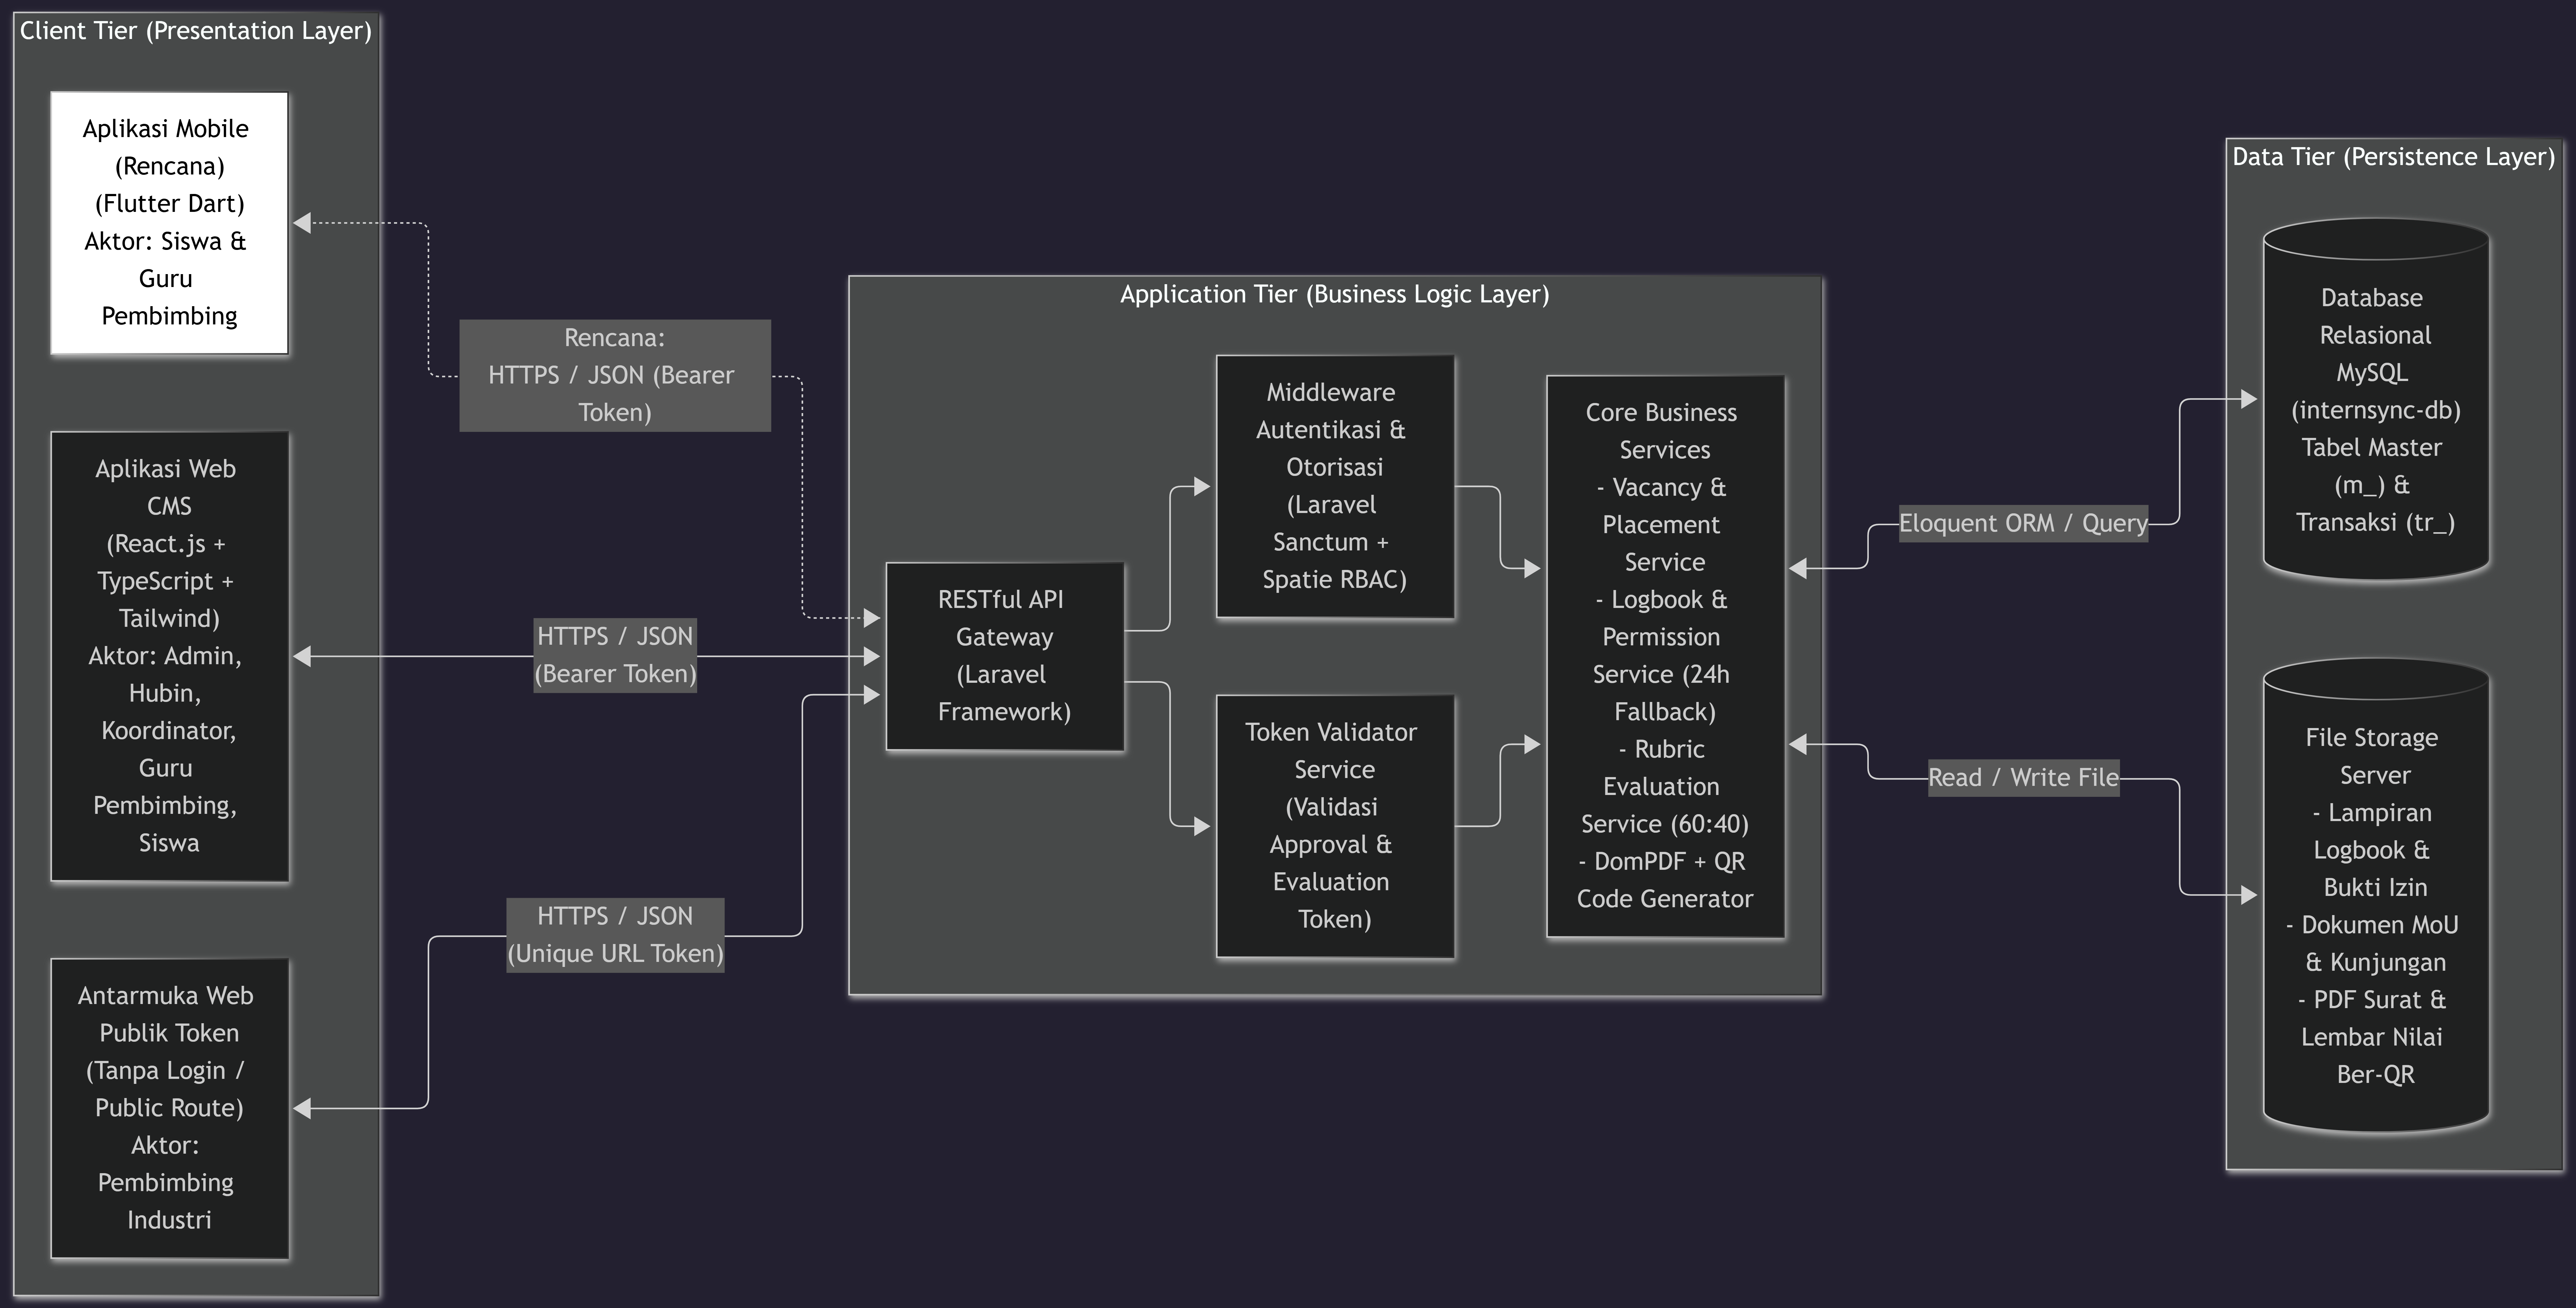
\includegraphics[width=12.39cm,height=0.78\textheight,keepaspectratio]{gambar/gambar-3-01.png}
\caption{Desain Arsitektur Sistem}\label{fig:3.1}
\end{figure}

Berdasarkan Gambar 3.1, proses komunikasi data dimulai ketika aplikasi web (dan kelak aplikasi mobile) mengirimkan permintaan melalui protokol HTTPS dalam format JSON yang diamankan dengan \textit{Bearer Token}, sedangkan antarmuka publik industri berkomunikasi menggunakan parameter \textit{Unique URL Token}. Seluruh permintaan diterima oleh \textit{RESTful API Gateway} berbasis framework Laravel pada \textit{Application Tier}. Permintaan dari aktor berakun akan melewati \textit{Middleware Autentikasi dan Otorisasi} (Laravel Sanctum dan Spatie RBAC), sementara akses publik industri akan divalidasi oleh \textit{Token Validator Service}. Selanjutnya, permintaan diproses oleh \textit{Core Business Services} yang mencakup layanan katalog lowongan dan penempatan, layanan \textit{self-reporting logbook} dan perizinan dengan aturan \textit{fallback} 24 jam, layanan evaluasi rubrik (rasio 60:40), serta generator dokumen DomPDF dan QR Code. Pada lapisan \textit{Data Tier}, sistem memanfaatkan Eloquent ORM untuk berkomunikasi dengan basis data relasional MySQL (\texttt{internsync-db}) yang memisahkan tabel master (\texttt{m\_}) dan tabel transaksi (\texttt{tr\_}), serta terhubung dengan \textit{File Storage Server} untuk menyimpan lampiran bukti logbook, surat izin, dokumen MoU, dan berkas PDF resmi ber-QR Code.

\subsection{Business Process Model and Notation (BPMN)}

BPMN digunakan untuk memberikan gambaran visual mengenai urutan aktivitas bisnis secara end-to-end yang melibatkan berbagai aktor di SMK PGRI Telagasari. Diagram ini memetakan kolaborasi antara Hubin, Koordinator, Pembimbing, dan Siswa dalam satu alur kerja terpadu.

\begin{figure}[H]
\centering
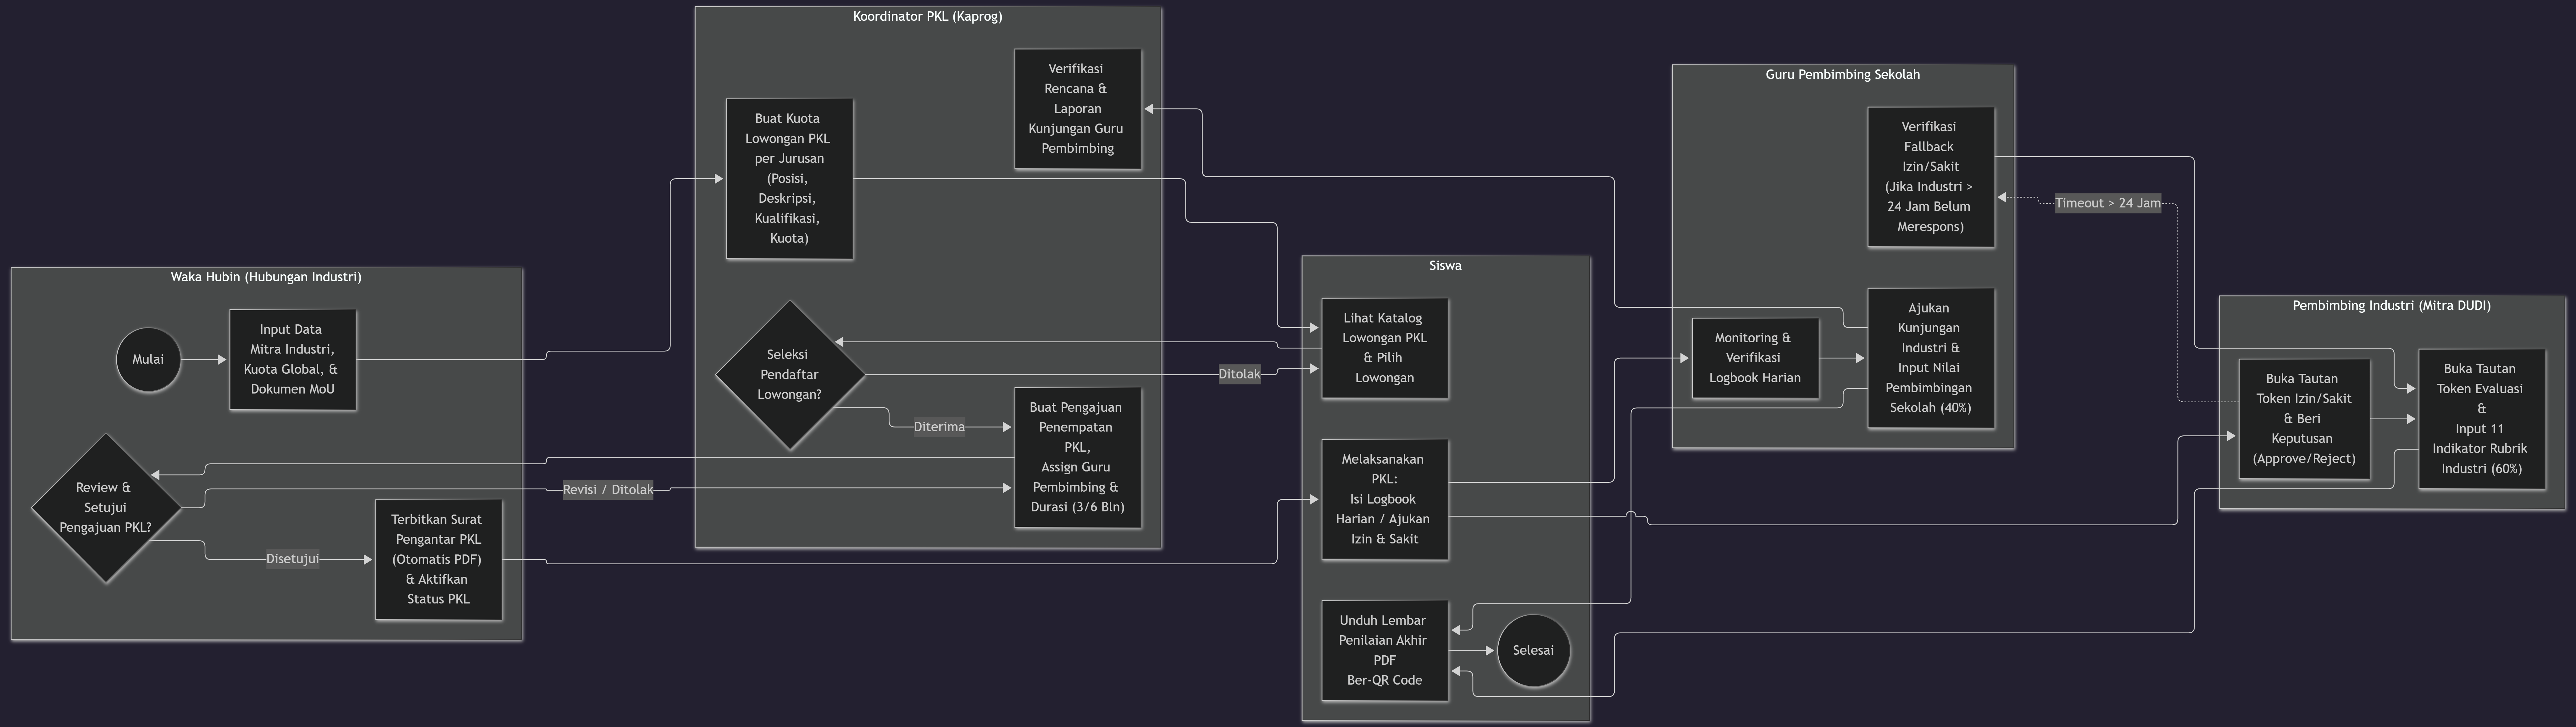
\includegraphics[width=13.98cm,height=0.78\textheight,keepaspectratio]{gambar/gambar-3-02.png}
\caption{Business Process Model and Notation (BPMN)}\label{fig:3.2}
\end{figure}

Berdasarkan Gambar~\ref{fig:3.2}, alur bisnis dimulai dari Waka Hubin yang menginput data master mitra industri serta dokumen MoU. Koordinator PKL kemudian mengatur lowongan PKL pada industri tersebut yang mencakup kuota, jenis lowongan (umum atau khusus jurusan), posisi, dan deskripsi. Siswa melihat katalog lowongan dan mengajukan lamaran pada lowongan yang diminati, lalu Koordinator menyeleksi siswa pendaftar lowongan tersebut. Apabila ditolak, siswa dapat memilih kembali lowongan lain yang tersedia; apabila diterima, Koordinator membuat dokumen pengajuan dan pengiriman PKL disertai penunjukan Guru Pembimbing dan penetapan durasi (3 atau 6 bulan) untuk ditinjau oleh Waka Hubin. Jika disetujui, Hubin menerbitkan Surat Pengantar PKL otomatis berformat PDF dan mengaktifkan status PKL siswa.

Selama masa pelaksanaan PKL, siswa mengisi \textit{logbook} harian secara mandiri atau mengajukan permohonan izin dan sakit. Catatan \textit{logbook} harian dipantau oleh Guru Pembimbing Sekolah dan dapat diekspor menjadi rekapitulasi PDF ber-QR Code, sedangkan permohonan izin/sakit diteruskan kepada Pembimbing Industri melalui tautan token untuk diberikan keputusan (\textit{approve/reject}). Apabila dalam waktu lebih dari 24 jam pihak industri belum merespons (\textit{timeout}), wewenang verifikasi izin dialihkan ke mekanisme \textit{fallback} oleh Guru Pembimbing Sekolah. Selain itu, Guru Pembimbing melaksanakan kunjungan industri berdasarkan jadwal Surat Perintah Perjalanan Dinas (SPPD) yang ditetapkan oleh Koordinator PKL. Pada tahap akhir, Pembimbing Industri menginput nilai pada 9 indikator rubrik industri (bobot 60\%) melalui tautan token evaluasi, dan Guru Pembimbing menginput nilai pada 2 indikator akademik sekolah (bobot 40\%), sehingga total terdapat 11 indikator penilaian. Setelah seluruh indikator terisi, sistem menghitung nilai akhir sehingga siswa dapat melihatnya serta mengunduh lembar penilaian berformat PDF.

\subsection{Use Case Diagram}

Use Case Diagram menggambarkan fungsionalitas sistem dari perspektif pengguna. Diagram ini mendefinisikan batasan sistem dan interaksi aktor terhadap fitur-fitur utama yang dikembangkan.

\begin{figure}[H]
\centering
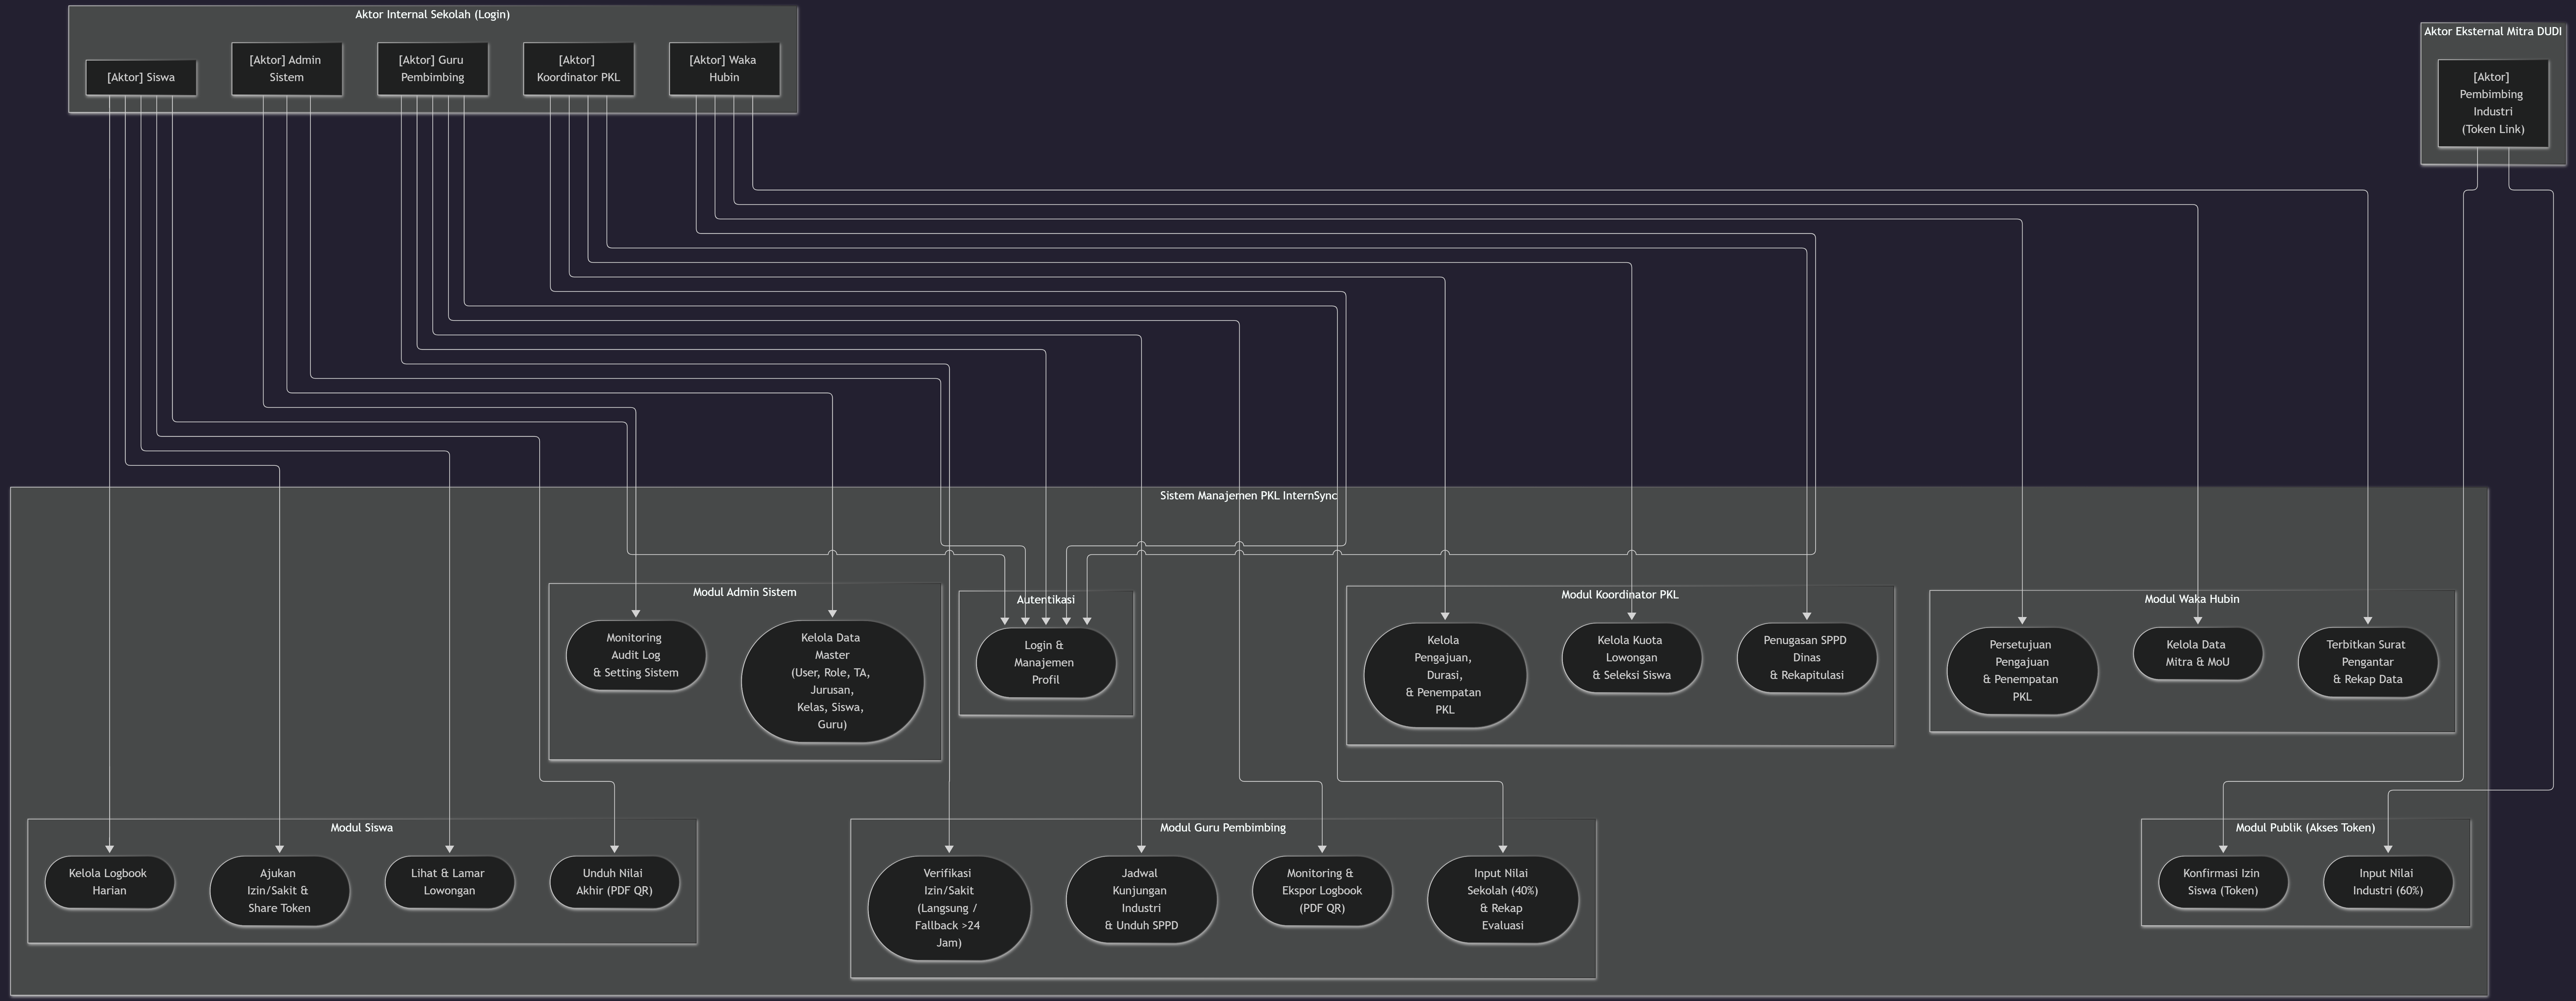
\includegraphics[width=13.98cm,height=0.78\textheight,keepaspectratio]{gambar/gambar-3-03.png}
\caption{Use Case Diagram}\label{fig:3.3}
\end{figure}

Terdapat lima aktor internal sekolah yang memiliki akun login dan satu aktor eksternal mitra DUDI tanpa login, dengan rincian fungsionalitas per modul sebagai berikut:

\begin{enumerate}[label=\alph*.]
\item \textbf{Admin Sistem:} Mengakses modul autentikasi (login dan manajemen profil), mengelola seluruh data master sistem (meliputi data \textit{user}, \textit{role}, tahun ajaran, jurusan, kelas, siswa, dan guru), serta melakukan \textit{monitoring audit log} dan pengaturan sistem.
\item \textbf{Waka Hubin (Hubungan Industri):} Mengakses modul autentikasi, mengelola data mitra industri dan dokumen MoU, melakukan persetujuan pengajuan dan penempatan PKL dari koordinator, serta menerbitkan surat pengantar PKL resmi dan memantau rekap data PKL.
\item \textbf{Koordinator PKL:} Mengakses modul autentikasi, mengelola kuota lowongan PKL dan menyeleksi siswa pendaftar, mengelola pengajuan, pengiriman, dan durasi PKL (3 atau 6 bulan), serta mengelola penugasan perjalanan dinas (SPPD) dan rekapitulasi laporan.
\item \textbf{Guru Pembimbing:} Mengakses modul autentikasi, melakukan \textit{monitoring} dan mengekspor \textit{logbook} harian siswa ke format PDF ber-QR Code, memverifikasi izin/sakit siswa (secara langsung maupun melalui mekanisme \textit{fallback} lebih dari 24 jam), melihat jadwal kunjungan industri dan mengunduh SPPD, serta menginput nilai sekolah (40\%) dan merekap evaluasi siswa.
\item \textbf{Siswa:} Mengakses modul autentikasi, melihat dan mengajukan lamaran pada katalog lowongan PKL, menginput dan mengelola \textit{logbook} harian secara mandiri, mengajukan permohonan izin/sakit beserta pembagian tautan token konfirmasi, serta melihat dan mengunduh lembar penilaian akhir berformat PDF ber-QR Code.
\item \textbf{Pembimbing Industri (Aktor Eksternal Mitra DUDI):} Berinteraksi tanpa login melalui modul publik berbasis tautan token untuk mengonfirmasi permohonan izin/sakit siswa serta menginput rubrik penilaian kinerja industri (bobot 60\%).
\end{enumerate}

\subsection{Activity Diagram}

Activity Diagram digunakan untuk menggambarkan alur aktivitas yang terjadi dalam sistem monitoring PKL berdasarkan interaksi antara pengguna dengan sistem. Diagram ini memodelkan proses yang dilakukan oleh setiap aktor melalui beberapa partisi atau swimlane yang menunjukkan pihak yang bertanggung jawab terhadap aktivitas tertentu. Dengan menggunakan Activity Diagram, alur proses sistem dapat dipahami secara lebih jelas mulai dari awal aktivitas hingga proses berakhir.

\subsubsection{Activity Diagram Login}

Activity Diagram login menggambarkan proses autentikasi pengguna sebelum dapat mengakses sistem monitoring PKL. Proses ini melibatkan interaksi antara pengguna yang memasukkan kredensial dan sistem yang melakukan validasi data.

\begin{figure}[H]
\centering
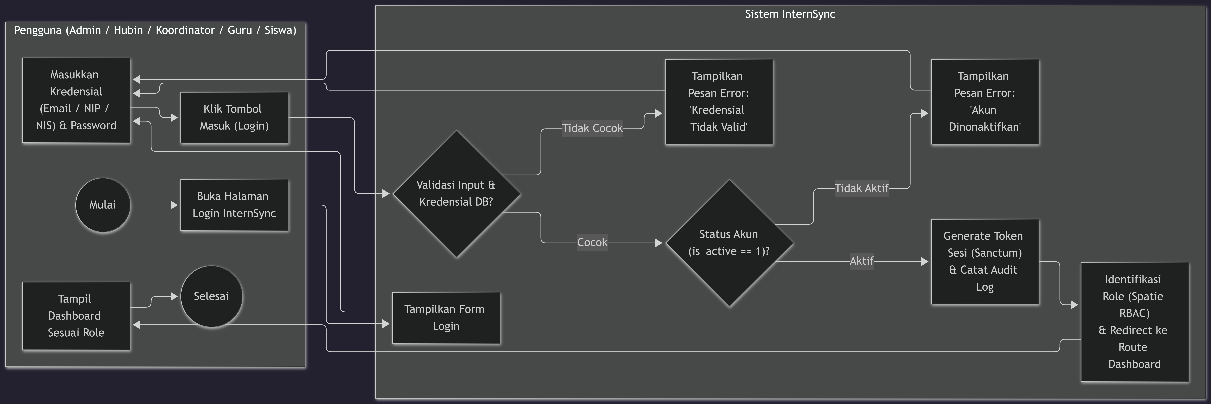
\includegraphics[width=13.98cm,height=0.78\textheight,keepaspectratio]{gambar/gambar-3-04.png}
\caption{Activity Diagram Login}\label{fig:3.4}
\end{figure}

Berdasarkan Gambar 3.4, proses dimulai ketika pengguna membuka halaman login InternSync, lalu sistem menampilkan formulir login. Pengguna memasukkan kredensial berupa Email, NIP, atau NIS beserta kata sandi dan menekan tombol masuk. Sistem melakukan validasi kecocokan kredensial terhadap basis data; apabila tidak cocok, sistem menampilkan pesan kesalahan \textit{Kredensial Tidak Valid} dan mengembalikan pengguna ke formulir login. Apabila kredensial cocok, sistem memeriksa status keaktifan akun (\texttt{is\_active == 1}). Jika akun berstatus tidak aktif, sistem menolak akses dan menampilkan pesan \textit{Akun Dinonaktifkan}. Jika akun aktif, sistem membuat token sesi autentikasi melalui Laravel Sanctum, mencatat aktivitas ke dalam tabel \textit{audit log}, mengidentifikasi peran pengguna melalui Spatie RBAC, dan mengarahkan pengguna ke halaman dasbor sesuai perannya masing-masing.

\subsubsection{Activity Diagram Katalog Lowongan dan Penempatan PKL}

Activity Diagram ini memvisualisasikan alur pengelolaan lowongan hingga penempatan siswa ke industri mitra. Proses ini penting untuk memastikan setiap siswa terdata secara sistematis di tempat pelaksanaan magang yang sesuai dengan keahliannya.

\begin{figure}[H]
\centering
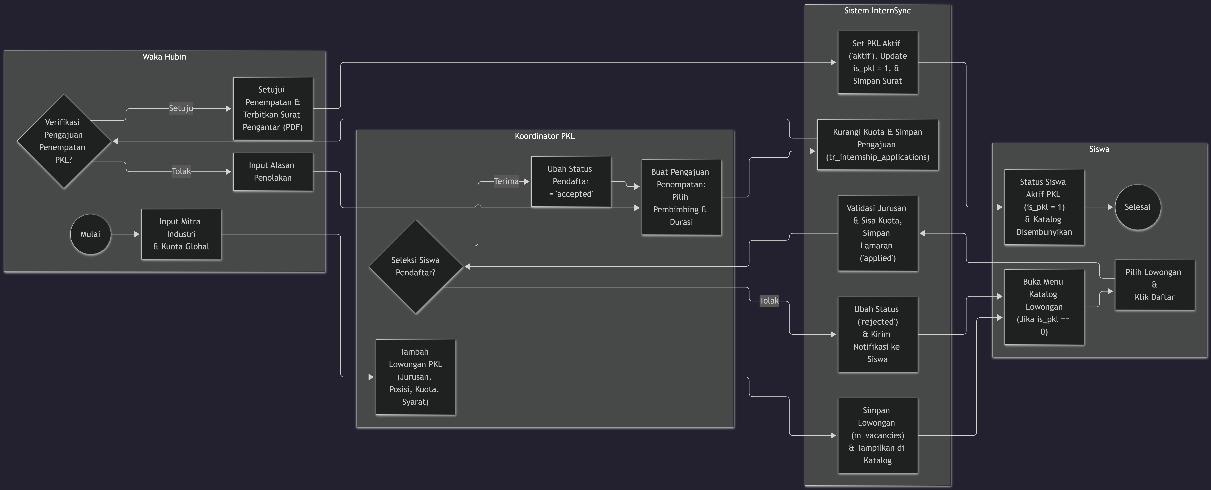
\includegraphics[width=13.98cm,height=0.78\textheight,keepaspectratio]{gambar/gambar-3-05.png}
\caption{Activity Diagram Katalog Lowongan dan Penempatan PKL}\label{fig:3.5}
\end{figure}

Proses diawali ketika Hubin menambahkan data industri mitra. Koordinator kemudian mengatur lowongan pada industri tersebut, meliputi kuota, jenis lowongan (umum atau khusus), posisi, dan deskripsi lowongan. Siswa dapat melihat katalog lowongan dan memilih lowongan yang diminati. Selanjutnya Koordinator menyeleksi siswa yang memilih lowongan, menetapkan penempatan beserta durasi pelaksanaan (3 atau 6 bulan), dan menunjuk guru pembimbing. Sistem memvalidasi input tersebut dan menyimpan dokumen pengajuan. Apabila validasi berhasil, pengajuan diteruskan kepada Hubin untuk disetujui, sehingga status magang siswa tercatat secara resmi untuk periode tersebut.

\subsubsection{Activity Diagram Pengisian Logbook}

Activity Diagram pengisian logbook menguraikan tahapan pencatatan aktivitas harian yang wajib dilakukan oleh siswa selama masa PKL. Logbook digital ini berfungsi sebagai portofolio capaian kompetensi harian yang dipantau secara berkala oleh guru pembimbing.

\begin{figure}[H]
\centering
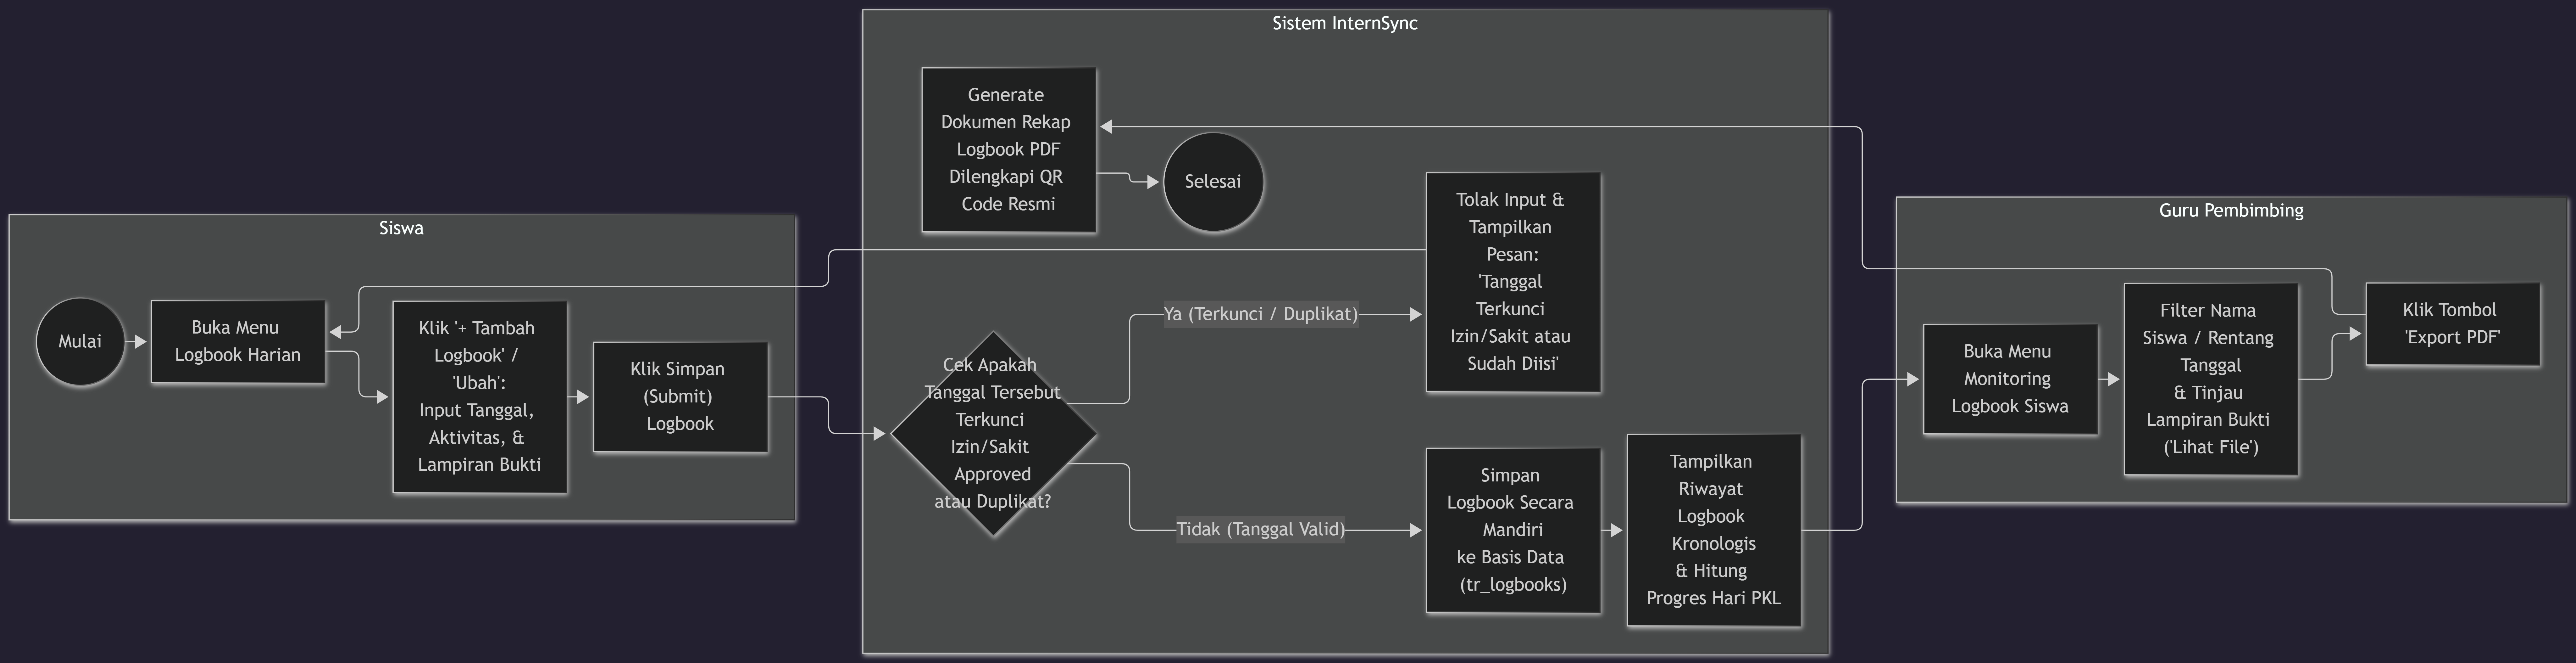
\includegraphics[width=13.98cm,height=0.78\textheight,keepaspectratio]{gambar/gambar-3-06.png}
\caption{Activity Diagram Pengisian Logbook}\label{fig:3.6}
\end{figure}

Berdasarkan Gambar 3.6, alur dimulai ketika siswa membuka menu \textit{logbook} harian dan menekan tombol tambah atau ubah \textit{logbook} untuk menginput tanggal, rincian aktivitas kerja, serta mengunggah berkas bukti pendukung. Setelah siswa menekan tombol simpan (\textit{submit}), sistem memeriksa apakah tanggal yang dipilih terkunci oleh status permohonan izin/sakit yang telah disetujui (\textit{approved}) atau telah terisi sebelumnya (duplikat). Apabila tanggal terkunci atau duplikat, sistem menolak input dan menampilkan pesan peringatan. Apabila tanggal valid, sistem langsung menyimpan catatan \textit{logbook} secara mandiri ke dalam tabel \texttt{tr\_logbooks}, menampilkan riwayat \textit{logbook} secara kronologis, serta memperbarui kalkulasi progres hari pelaksanaan PKL siswa. Selanjutnya, Guru Pembimbing dapat memantau seluruh entri aktivitas melalui menu \textit{monitoring logbook}, memfilter berdasarkan nama siswa atau rentang tanggal, meninjau lampiran bukti kegiatan, dan menekan tombol ekspor PDF untuk menghasilkan dokumen rekapitulasi \textit{logbook} resmi ber-QR Code.

\subsubsection{Activity Diagram Pengajuan Izin dan Sakit}

Activity Diagram pengajuan izin dan sakit mengatur mekanisme pelaporan ketidakhadiran siswa agar akuntabilitas kehadiran tetap terjaga tanpa menghambat operasional industri.

\begin{figure}[H]
\centering
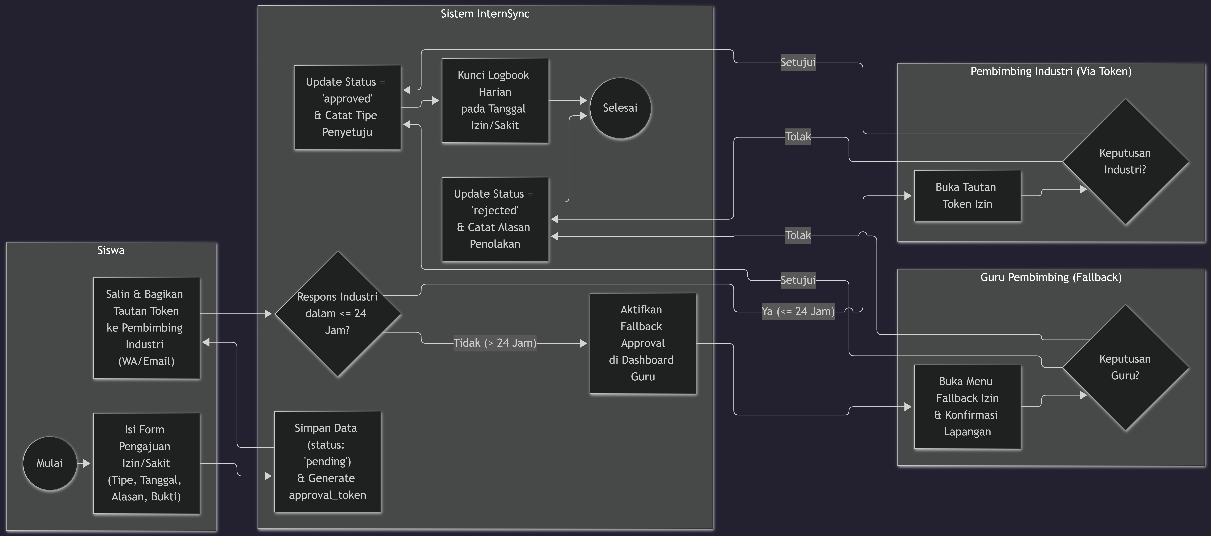
\includegraphics[width=13.99cm,height=0.78\textheight,keepaspectratio]{gambar/gambar-3-07.png}
\caption{Activity Diagram Pengajuan Izin dan Sakit}\label{fig:3.7}
\end{figure}

Alur dimulai saat siswa berhalangan hadir dan mengisi form perizinan pada sistem dengan memilih jenis ketidakhadiran (izin atau sakit), rentang tanggal, alasan, serta mengunggah dokumen bukti otentik (surat keterangan dokter atau surat izin orang tua). Sistem memvalidasi data dan secara otomatis mengirimkan notifikasi tautan ber-token aman kepada pembimbing industri. Pembimbing industri dapat langsung membuka tautan tersebut pada peramban ponsel dan memberikan persetujuan (approve/reject) dalam satu klik tanpa perlu melakukan login akun. Apabila dalam kurun waktu 24 jam pembimbing industri belum memberikan tanggapan, guru pembimbing sekolah memiliki hak akses fallback untuk memverifikasi izin tersebut secara langsung berdasarkan keabsahan dokumen bukti. Perizinan yang telah disetujui akan secara otomatis mengunci formulir logbook pada tanggal terkait sehingga siswa tidak tercatat alpa.

\subsubsection{Activity Diagram Evaluasi PKL}

Activity Diagram evaluasi PKL menggambarkan mekanisme penilaian akhir berbasis rubrik baku yang menjadi tolak ukur pencapaian kompetensi dan keberhasilan praktik kerja lapangan.

\begin{figure}[H]
\centering
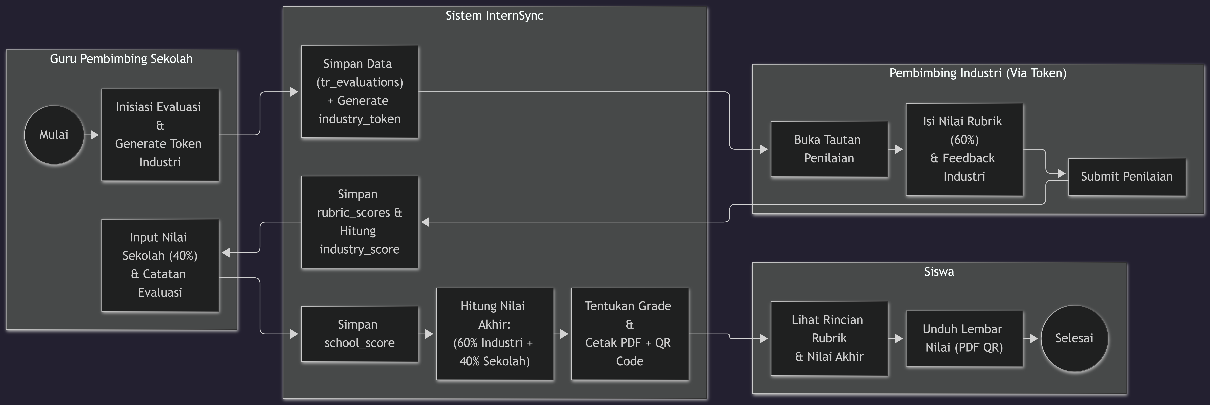
\includegraphics[width=13.97cm,height=0.78\textheight,keepaspectratio]{gambar/gambar-3-08.png}
\caption{Activity Diagram Evaluasi PKL}\label{fig:3.8}
\end{figure}

Evaluasi PKL mengadopsi standar rubrik baku jurnal PKL SMK dengan total 11 indikator dalam tiga kelompok. Kelompok A, aspek sikap dan non-teknis (5 indikator, dinilai industri), meliputi kedisiplinan dan kehadiran, tanggung jawab dan kejujuran, inisiatif dan kemandirian, etika kerja dan komunikasi tim, serta penerapan prosedur K3LH. Kelompok B, aspek keterampilan dan teknis (4 indikator, dinilai industri), meliputi penguasaan peralatan dan tooling industri, kualitas dan presisi hasil pekerjaan, kemampuan analisis dan pemecahan masalah, serta kecepatan dan ketuntasan tugas kerja. Kelompok C, aspek akademik dan laporan (2 indikator, dinilai sekolah), meliputi sistematika dan kelengkapan laporan akhir PKL serta penguasaan materi dan presentasi pertanggungjawaban. Pembimbing industri mengisi 9 indikator kelompok A dan B melalui tautan evaluasi aman, atau melalui lembar fisik yang kemudian diinputkan ke sistem oleh guru pembimbing saat kunjungan supervisi akhir, sedangkan guru pembimbing sekolah mengisi 2 indikator kelompok C. Sistem secara otomatis menghitung nilai industri dari 9 indikator dan nilai sekolah dari 2 indikator, menggabungkannya dengan bobot 60\% dan 40\% menjadi nilai akhir, mengonversinya ke predikat huruf (A, B, C, D), dan menerbitkan lembar penilaian akhir resmi yang dapat diakses dan diunduh siswa melalui dasbor masing-masing.

\subsection{Entity Relationship Diagram (ERD)}

Entity Relationship Diagram (ERD) merelasikan struktur basis data yang membentuk sistem monitoring PKL. Diagram ini memetakan entitas pengguna, siswa, industri, hingga pelaporan untuk memastikan komponen data saling terhubung dan terintegrasi dalam mendukung proses bisnis.

\begin{figure}[H]
\centering
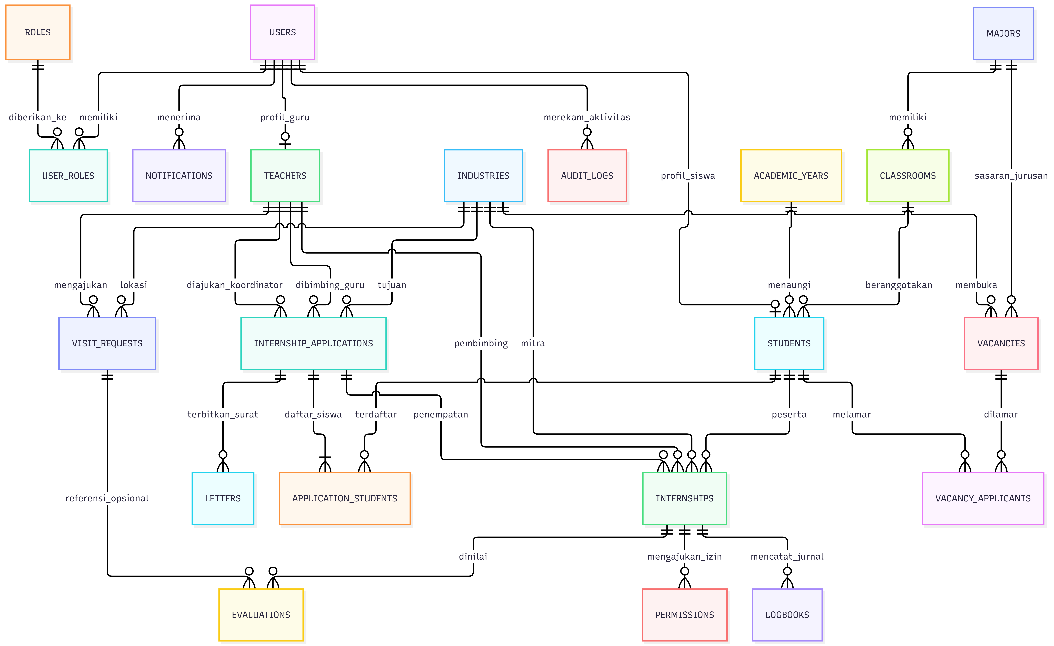
\includegraphics[width=12.17cm,height=0.78\textheight,keepaspectratio]{gambar/gambar-3-09.png}
\caption{Entity Relationship Diagram (ERD)}\label{fig:3.9}
\end{figure}

Berdasarkan Gambar 3.9, struktur entitas sistem menggunakan \texttt{USERS}, \texttt{ROLES}, dan \texttt{USER\_ROLES} untuk mengelola autentikasi dan hak akses multi-peran. Profil pengguna akademik dipetakan ke dalam entitas \texttt{STUDENTS} dan \texttt{TEACHERS}, yang didukung oleh entitas struktur akademik meliputi \texttt{ACADEMIC\_YEARS}, \texttt{MAJORS}, dan \texttt{CLASSROOMS}. Data kemitraan perusahaan disimpan pada entitas \texttt{INDUSTRIES}, yang berelasi dengan entitas \texttt{VACANCIES} dan \texttt{VACANCY\_APPLICANTS} untuk memfasilitasi katalog lowongan PKL serta seleksi pendaftar oleh koordinator. Proses pengajuan penempatan kelompok siswa dikelola melalui entitas \texttt{INTERNSHIP\_APPLICATIONS} dan \texttt{APPLICATION\_STUDENTS}, yang kemudian menghasilkan penempatan aktif pada entitas pusat \texttt{INTERNSHIPS} serta penerbitan dokumen surat resmi pada \texttt{LETTERS}. Selama pelaksanaan PKL, pencatatan kegiatan harian disimpan pada \texttt{LOGBOOKS}, pengajuan izin/sakit ber-token pada \texttt{PERMISSIONS}, penugasan supervisi lapangan guru pada \texttt{VISIT\_REQUESTS}, dan penilaian akhir berbasis rubrik pada \texttt{EVALUATIONS}. Sebagai pendukung tata kelola sistem, entitas \texttt{NOTIFICATIONS} menangani pesan pemberitahuan pengguna dan \texttt{AUDIT\_LOGS} merekam jejak aktivitas krusial demi menjaga akuntabilitas data.

Perancangan ERD yang baik berperan penting dalam memastikan relasi antar entitas berjalan secara konsisten serta meminimalkan redundansi data pada sistem \cite{ref14}. Penerapan Physical Data Model yang dinormalisasi turut mendukung efisiensi proses query serta menjaga integritas referensial antar tabel dalam basis data relasional \cite{ref15}.

\subsection{Physical Data Model (PDM)}

Physical Data Model (PDM) merupakan wujud implementasi struktur basis data secara nyata pada DBMS. Pemodelan ini mendeskripsikan secara detail tabel, atribut, tipe data, serta primary key yang akan mendukung keseluruhan proses pelaporan dan administrasi dalam sistem.

\begin{figure}[H]
\centering
\includegraphics[width=13.99cm,height=0.78\textheight,keepaspectratio]{gambar/gambar-3-10.png}
\caption{Physical Data Model (PDM)}\label{fig:3.10}
\end{figure}

{\raggedright
Perancangan fisik basis data pada Gambar 3.10 memisahkan secara tegas antara sepuluh tabel master (berawalan \texttt{m\_}) dan sebelas tabel transaksi (berawalan \texttt{tr\_}). Tabel master menyimpan referensi data yang relatif statis, mencakup \texttt{m\_users}, \texttt{m\_roles}, \texttt{m\_user\_roles}, \texttt{m\_academic\_years}, \texttt{m\_majors}, \texttt{m\_classrooms}, \texttt{m\_students}, \texttt{m\_teachers}, \texttt{m\_industries}, serta \texttt{m\_vacancies} (menyimpan katalog lowongan beserta kuota dan relasi opsional \texttt{major\_id} untuk lowongan umum maupun khusus jurusan). Sebaliknya, tabel transaksi mengakomodasi aktivitas operasional yang dinamis, meliputi \texttt{tr\_vacancy\_applicants}, \texttt{tr\_internship\_applications}, \texttt{tr\_application\_students}, \texttt{tr\_internships}, \texttt{tr\_logbooks}, \texttt{tr\_permissions} (dilengkapi atribut \texttt{approval\_token} dan \texttt{approved\_by\_type} untuk mekanisme \textit{fallback}), \texttt{tr\_visit\_requests}, \texttt{tr\_evaluations} (menyimpan matriks 11 indikator pada kolom JSON \texttt{rubric\_scores} dengan bobot \texttt{industry\_score} 60\% dan \texttt{school\_score} 40\%), \texttt{tr\_letters}, \texttt{tr\_notifications}, serta \texttt{tr\_audit\_logs}. Seluruh relasi operasional pelaksanaan magang berpusat pada tabel \texttt{tr\_internships} yang telah dinormalisasi hingga \textit{Third Normal Form} (3NF) guna menjaga integritas referensial dan menghindari redundansi data.
\par}

\subsection{Gambaran Antarmuka Sistem}

Gambar pada subbab ini merupakan tangkapan layar antarmuka sistem InternSync yang telah diimplementasikan. Gambar dipertahankan sesuai urutan siklus pelaksanaan Praktik Kerja Lapangan (PKL), mulai dari autentikasi dan pengelolaan data, seleksi serta penempatan siswa, hingga monitoring, evaluasi, dan pelaporan. Rangkaian gambar memperlihatkan tampilan antarmuka sekaligus alur penggunaan sistem oleh Admin, Hubin, Koordinator PKL, Guru Pembimbing, Siswa, dan Pembimbing Industri.

\subsubsection{Fase Autentikasi dan Administrasi Master Sistem}

Fase ini merupakan fondasi operasional sistem yang mencakup gerbang akses terpusat bagi seluruh pengguna serta tata kelola data master entitas yang dibutuhkan sebelum aktivitas PKL dapat diselenggarakan.

\begin{figure}[H]
\centering
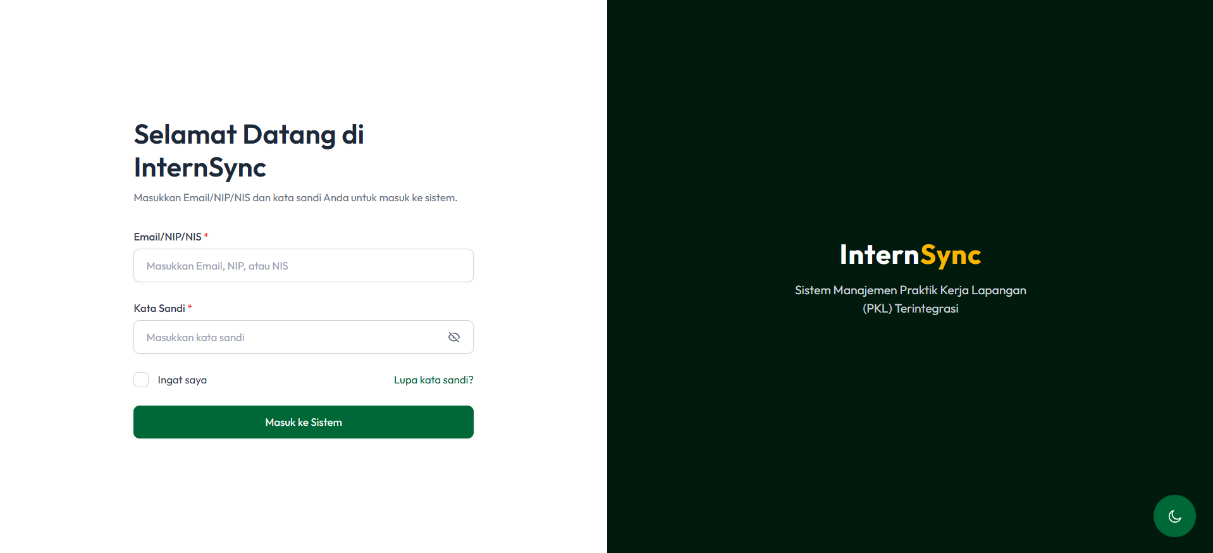
\includegraphics[width=14.00cm,height=0.78\textheight,keepaspectratio]{gambar/gambar-3-11.png}
\caption{Halaman Otentikasi (Login)}\label{fig:3.11}
\end{figure}

Antarmuka ini berfungsi sebagai pintu gerbang utama untuk mengakses sistem InternSync. Pengguna masuk dengan kredensial multiatribut berupa alamat email, NIP bagi tenaga pendidik, atau NIS bagi siswa, beserta kata sandi. Pada tampilan ini, formulir masuk di sisi kiri menyediakan fitur “Ingat Saya” dan opsi pemulihan kata sandi, sedangkan sisi kanan memuat logo InternSync, ilustrasi, dan ringkasan sistem. Sistem menggunakan Laravel Sanctum dan Spatie Role-Based Access Control (RBAC) untuk mengidentifikasi peran pengguna dan mengarahkan navigasi ke dasbor yang sesuai.

\begin{figure}[H]
\centering
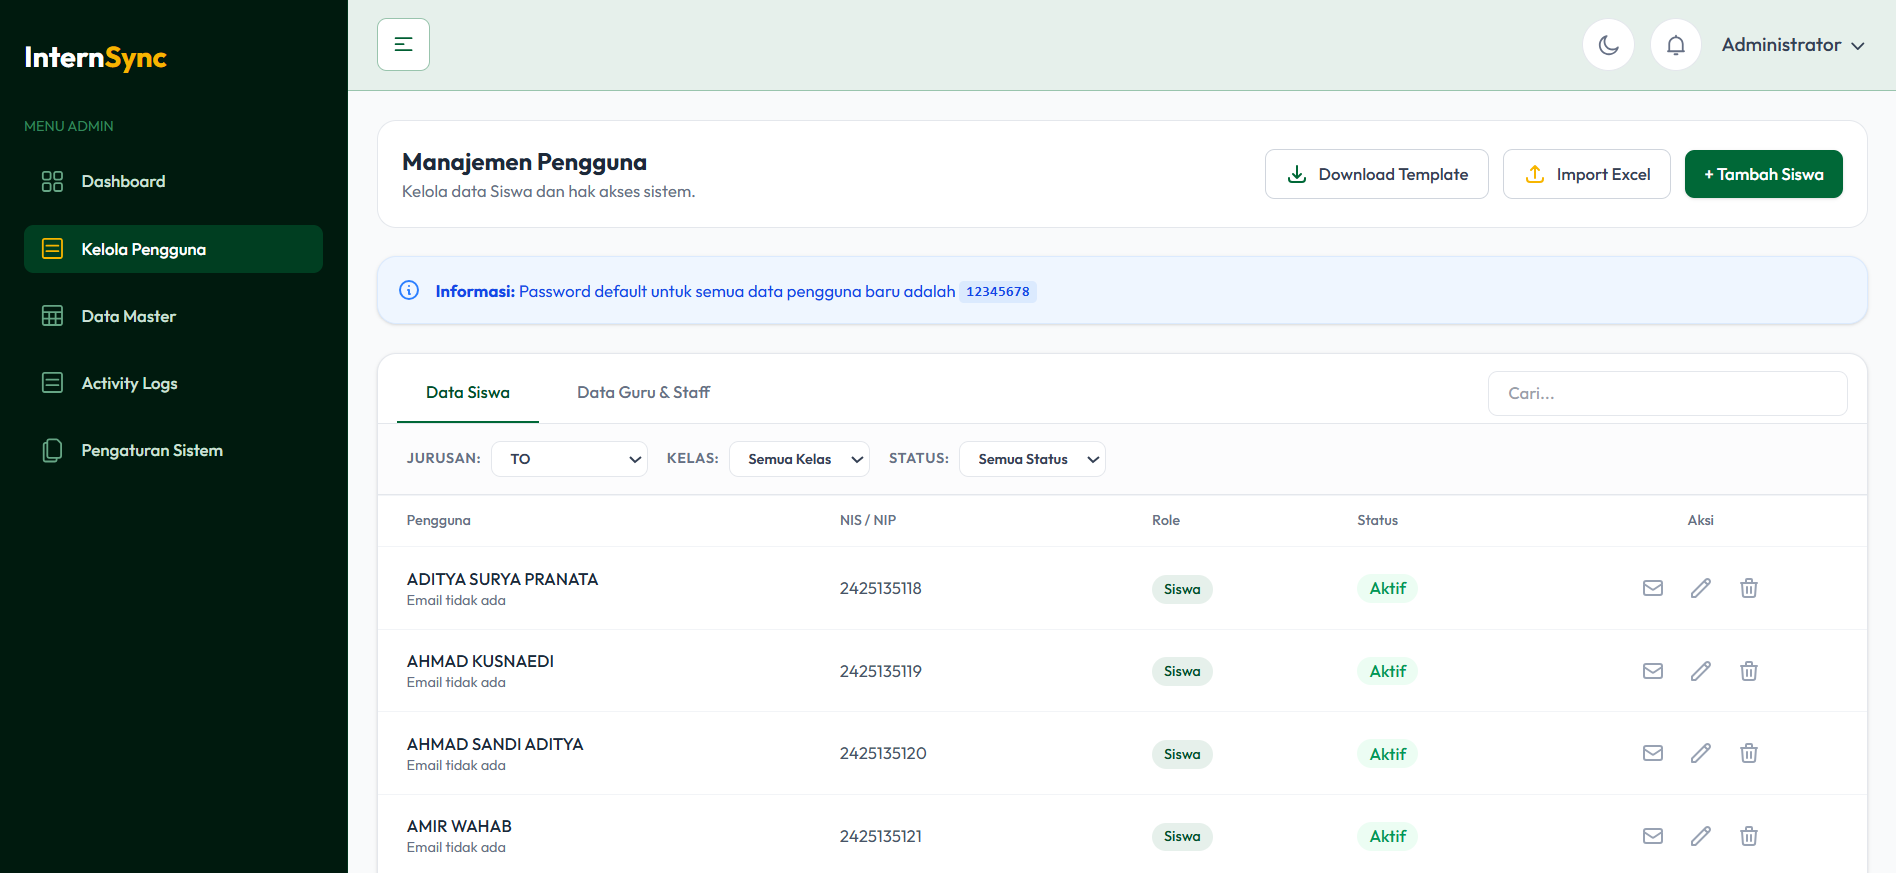
\includegraphics[width=14.00cm,height=0.78\textheight,keepaspectratio]{gambar/gambar-3-12.png}
\caption{Antarmuka Panel Administrasi dan Manajemen Pengguna (Admin)}\label{fig:3.12}
\end{figure}

Antarmuka ini merupakan pusat kendali manajemen akun yang diperuntukkan khusus bagi peran Admin Sistem pada menu Kelola Pengguna. Halaman ini memisahkan pengelolaan akun ke dalam dua tab terstruktur, yaitu tab Data Siswa dan tab Data Guru \& Staff, serta menampilkan informasi \textit{password default} bagi akun pengguna baru. Komponen utama antarmuka berupa \textit{data table} yang menyajikan daftar pengguna beserta atribut NIS/NIP, \textit{Role} (\textit{badge} Siswa/Guru), Status keaktifan akun (Aktif), serta kolom Aksi yang memuat tombol pintasan pengaturan email, ubah data (\textit{edit}), dan hapus akun. Untuk mempercepat migrasi data massal pada awal tahun ajaran, antarmuka ini dilengkapi fitur penyaringan berlapis (berdasarkan Jurusan, Kelas, dan Status), kolom pencarian cepat, serta tombol operasional \textit{Download Template}, \textit{Import Excel}, dan + Tambah Siswa di bagian kanan atas.

\begin{figure}[H]
\centering
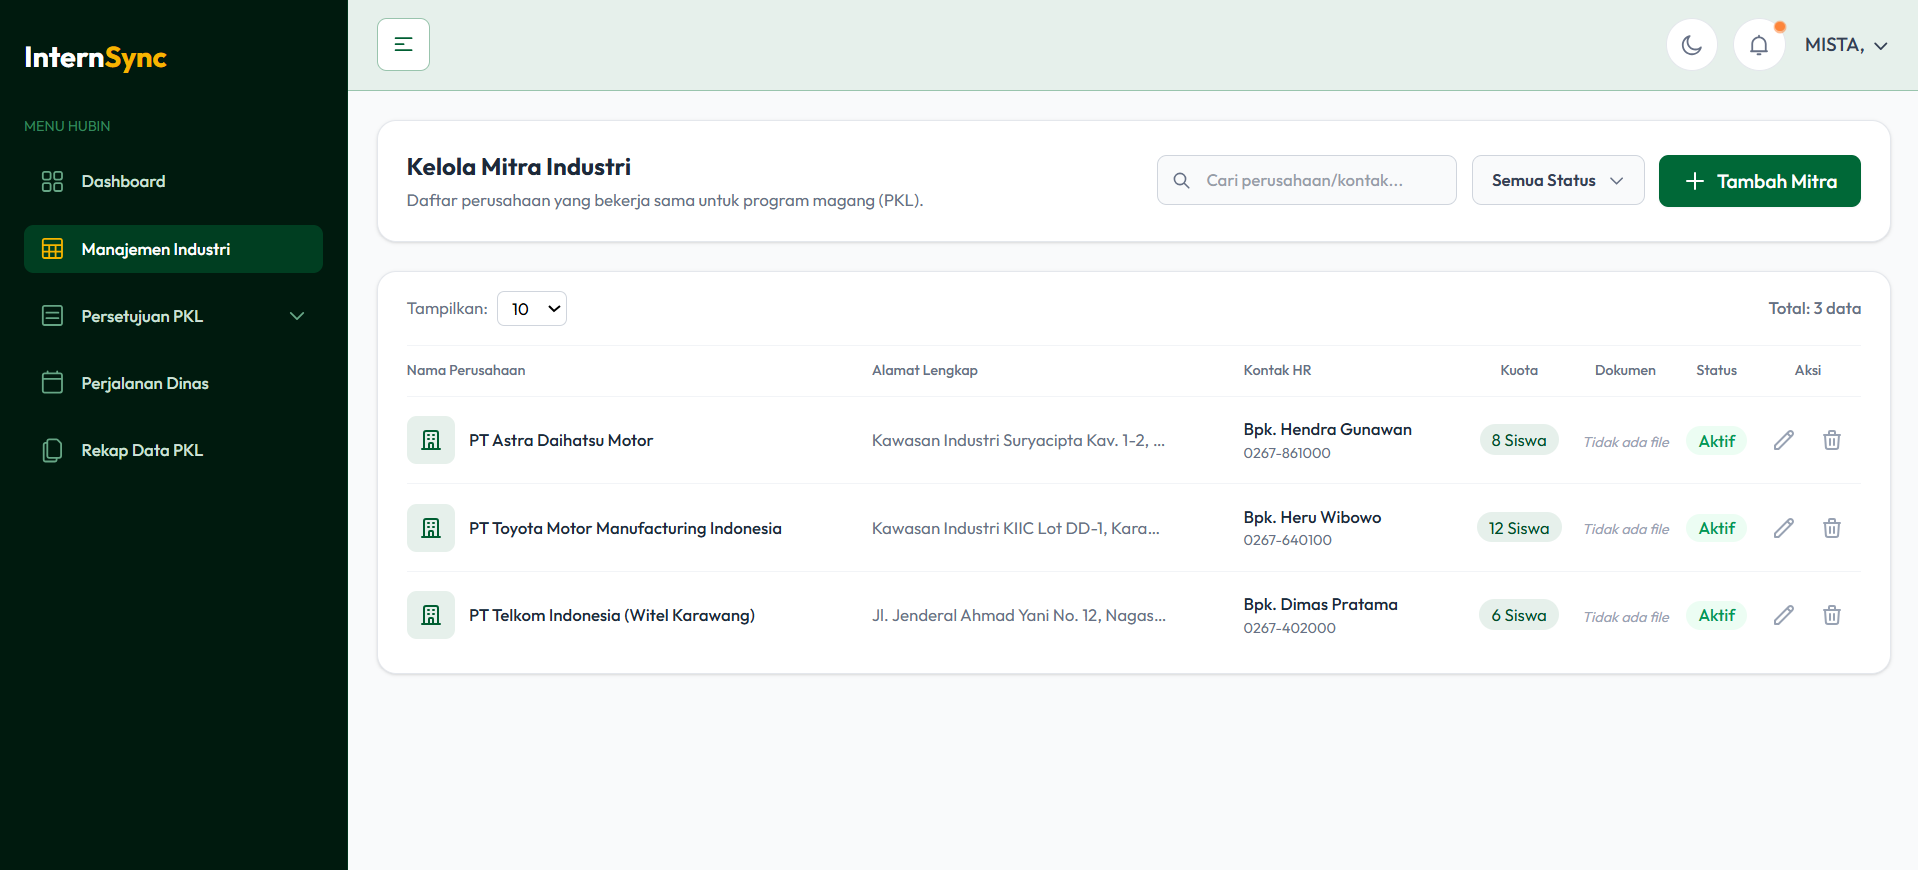
\includegraphics[width=14.00cm,height=0.78\textheight,keepaspectratio]{gambar/gambar-3-13.png}
\caption{Antarmuka Manajemen Mitra Industri dan Dokumen MoU (Hubin)}\label{fig:3.13}
\end{figure}

Antarmuka ini berfungsi sebagai modul tata kelola data master entitas dunia usaha dan dunia industri (DUDI) mitra yang berada di bawah wewenang Waka Hubin. Komponen utama menggunakan data table komprehensif yang memuat nama perusahaan, alamat operasional, kontak personal penanggung jawab/HR, status kerja sama aktif, serta kuota penempatan kumulatif. Dilengkapi dengan tombol aksi Tambah Mitra Baru, fasilitas unggah dokumen nota kesepahaman (MoU) legal dalam format digital, serta fitur modifikasi data secara inline. Ketersediaan data industri yang tervalidasi pada halaman ini menjadi prasyarat mutlak (prerequisite) bagi Koordinator PKL untuk dapat menginisiasi pembukaan lowongan PKL di tahap berikutnya.

\subsubsection{Fase Pra-PKL (Katalog Lowongan, Seleksi, Pengajuan, dan Penempatan)}

Fase ini mencakup rangkaian proses persiapan penempatan siswa, dimulai dari pembukaan kuota lowongan, pendaftaran mandiri oleh siswa, seleksi administratif, perumusan surat pengantar, hingga clearance keberangkatan resmi ke lokasi industri.

\begin{figure}[H]
\centering
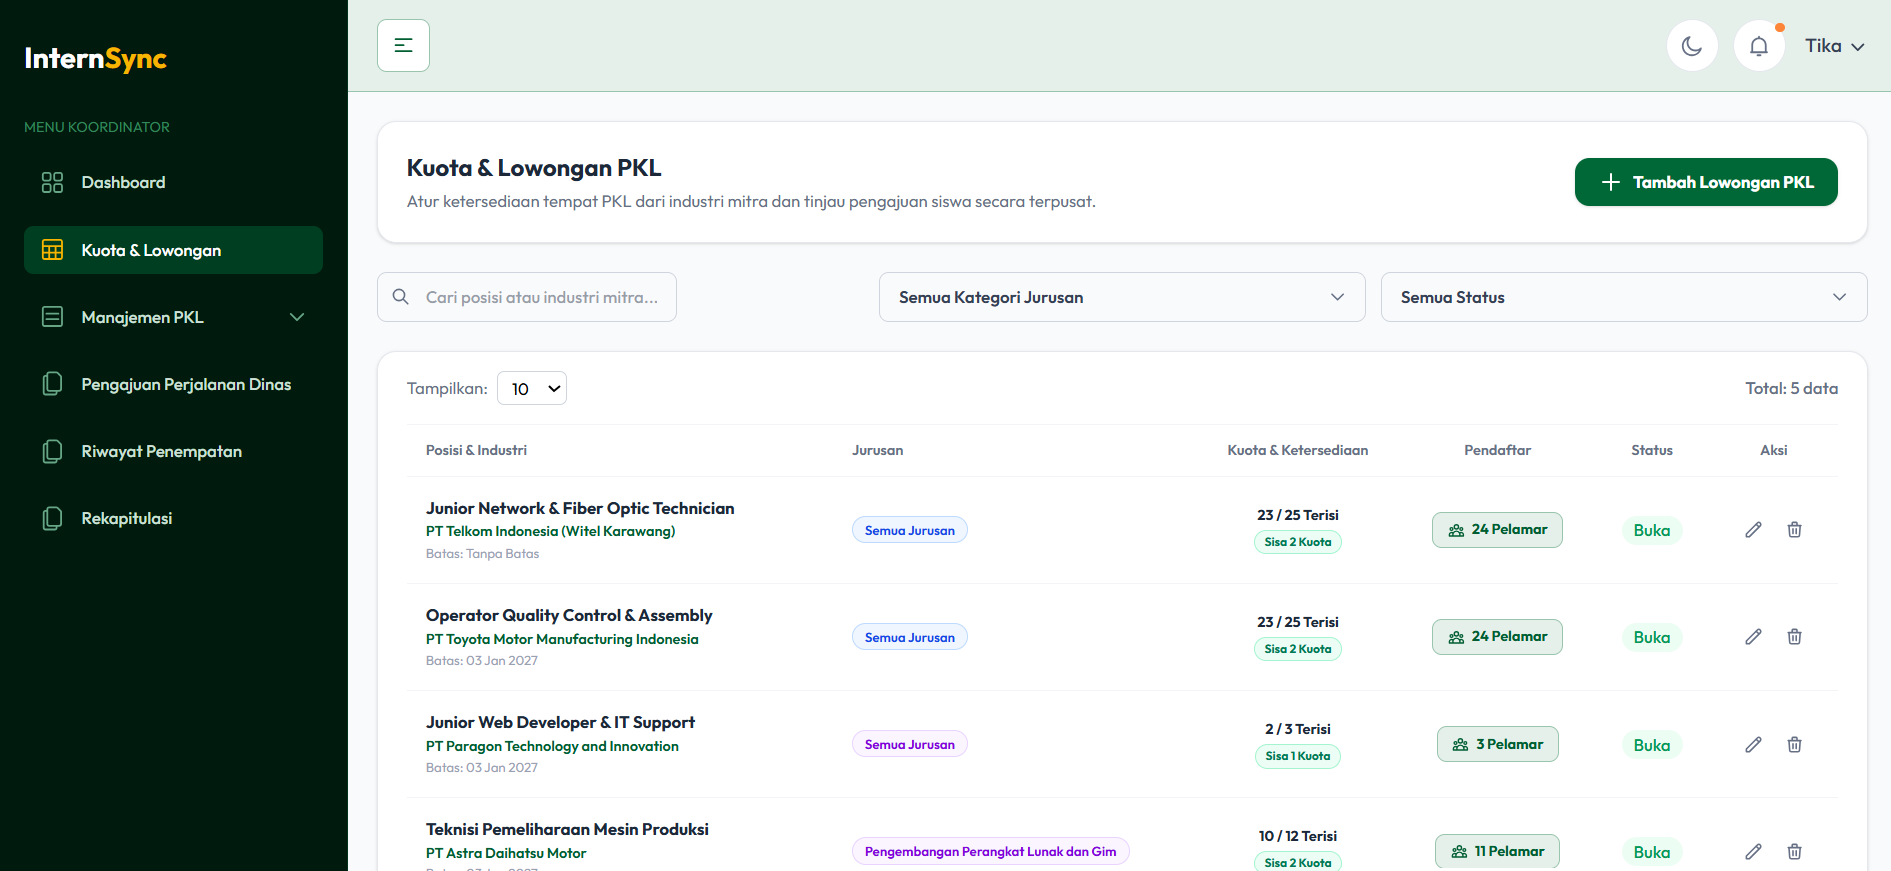
\includegraphics[width=14.00cm,height=0.78\textheight,keepaspectratio]{gambar/gambar-3-14.png}
\caption{Antarmuka Manajemen Lowongan PKL (Koordinator)}\label{fig:3.14}
\end{figure}

Halaman ini digunakan oleh Koordinator PKL untuk merumuskan dan mengelola lowongan magang berdasarkan daftar industri mitra yang telah disahkan oleh pihak Hubin. Antarmuka berbentuk data table dengan tombol inisiasi Tambah Lowongan. Formulir pembuatan lowongan mengintegrasikan elemen pilihan industri terikat, penentuan posisi pekerjaan (job role), kualifikasi keahlian yang disyaratkan, kuota kapasitas siswa yang dapat diterima, batas akhir pendaftaran (deadline), serta penentuan klasifikasi lowongan (lowongan umum untuk seluruh kompetensi keahlian atau lowongan khusus yang dibatasi untuk jurusan spesifik). Kolom aksi menyediakan opsi untuk mengubah rincian lowongan atau menutup status pendaftaran secara real-time.

\begin{figure}[H]
\centering
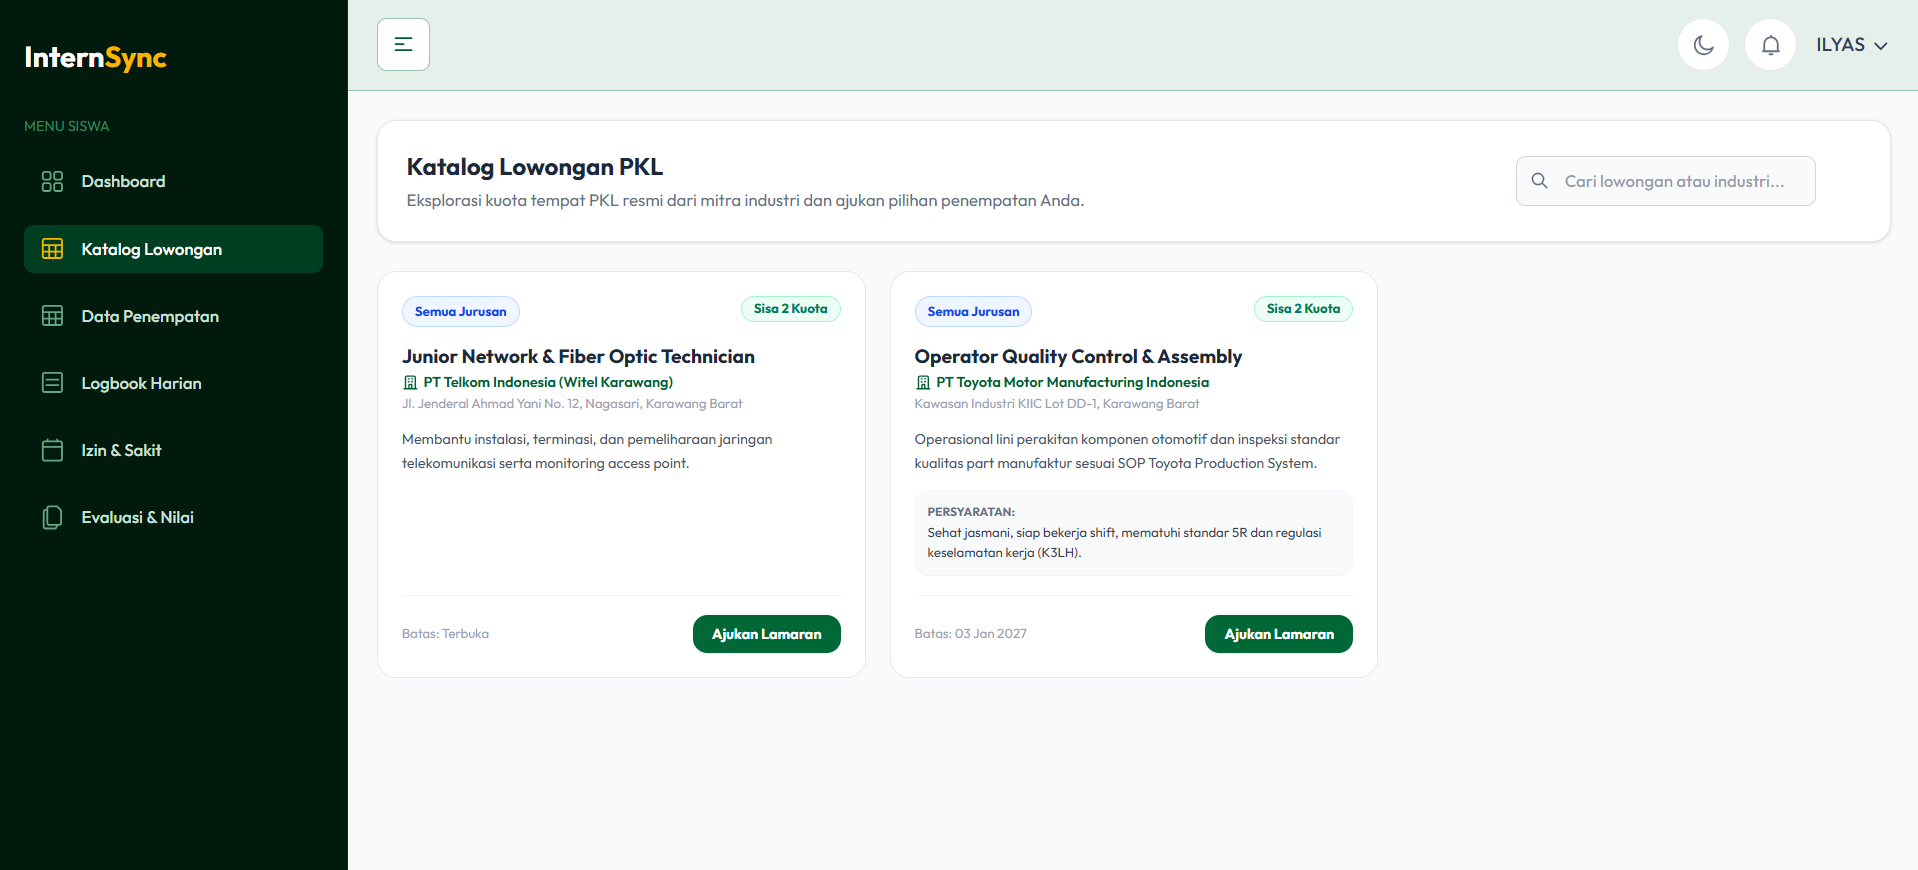
\includegraphics[width=14.00cm,height=0.78\textheight,keepaspectratio]{gambar/gambar-3-15.png}
\caption{Antarmuka Katalog dan Pendaftaran Lowongan PKL (Siswa)}\label{fig:3.15}
\end{figure}

Antarmuka ini menyajikan informasi seluruh peluang penempatan PKL aktif kepada siswa prakerin dalam format kartu interaktif (\textit{grid cards}) yang responsif dan informatif. Setiap kartu lowongan memvisualisasikan kategori jurusan (Semua Jurusan atau jurusan spesifik), indikator sisa kuota yang tersedia, judul posisi pekerjaan, nama dan alamat industri mitra, deskripsi tugas, kotak persyaratan khusus (seperti kepatuhan K3LH), serta batas waktu pendaftaran. Siswa dapat mencari lowongan melalui kolom pencarian di sudut kanan atas dan langsung mengajukan pendaftaran mandiri dengan menekan tombol Ajukan Lamaran pada kartu lowongan yang diminati. Sistem menyematkan validasi otomatis; tombol lamaran dinonaktifkan apabila kuota telah terisi penuh atau siswa telah berstatus aktif menjalani PKL.

\begin{figure}[H]
\centering
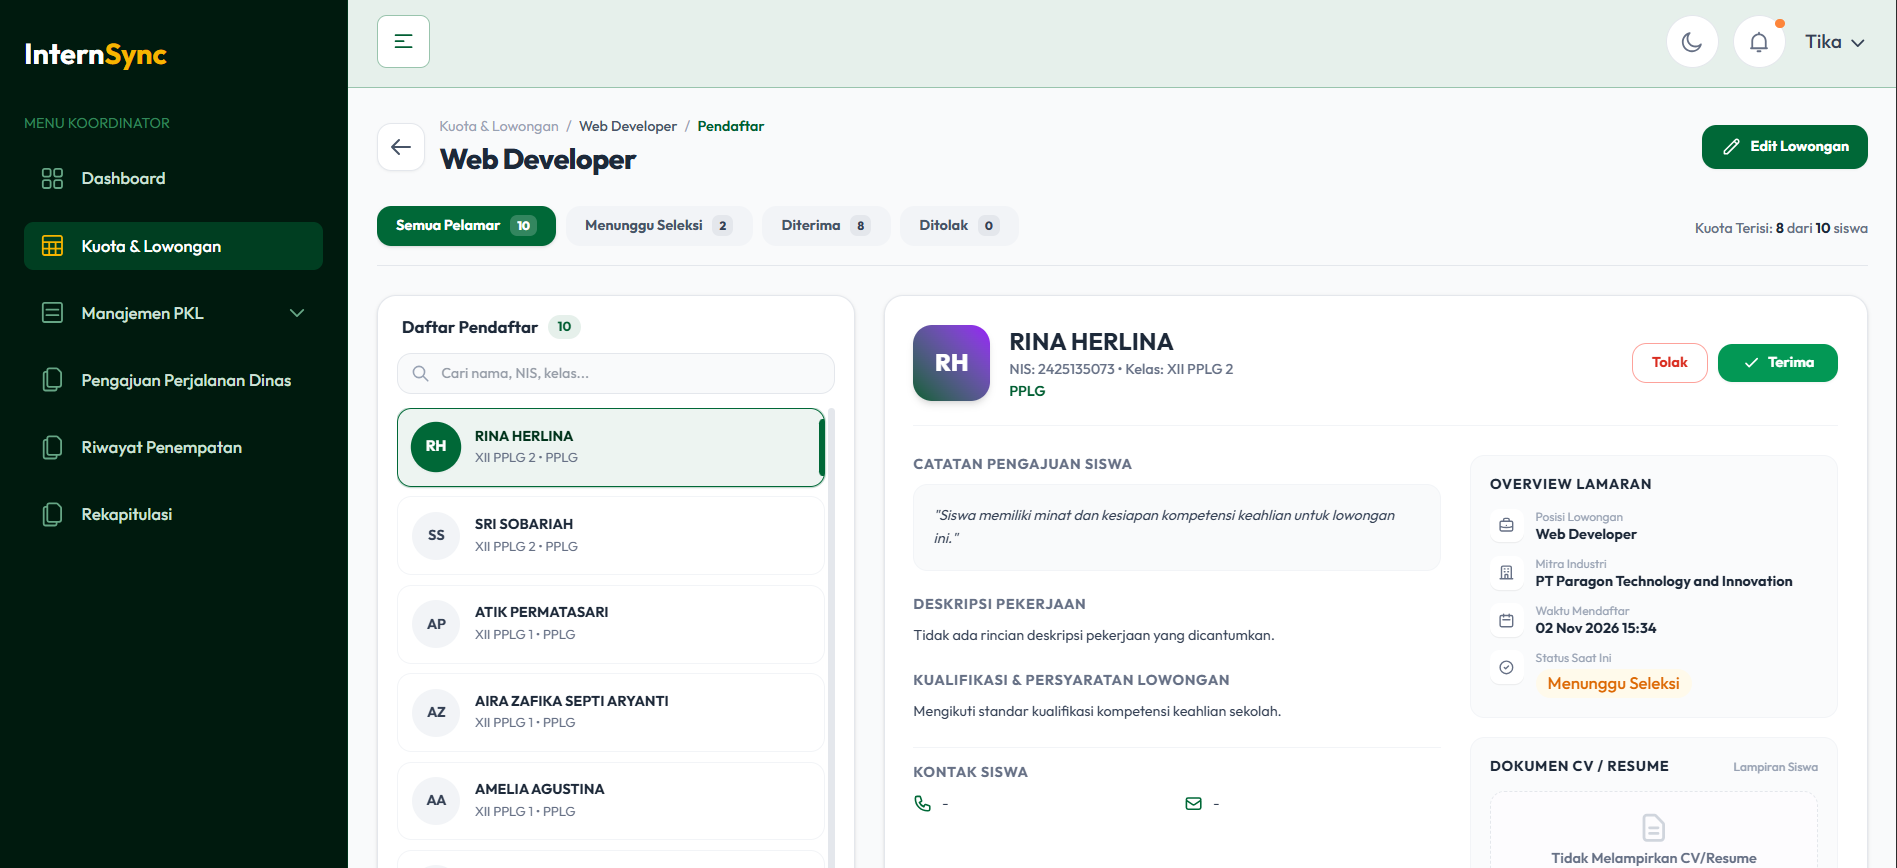
\includegraphics[width=14.00cm,height=0.78\textheight,keepaspectratio]{gambar/gambar-3-16.png}
\caption{Antarmuka Seleksi Pendaftar Lowongan (Koordinator)}\label{fig:3.16}
\end{figure}

Halaman ini merupakan decision support interface bagi Koordinator PKL untuk memverifikasi dan menyortir berkas permohonan siswa yang mendaftar pada setiap entitas lowongan. Antarmuka menyajikan daftar nominatif siswa pelamar yang dilengkapi metrik jurusan, kelas, dan tanggal pengajuan. Pada kolom aksi, Koordinator diberikan otoritas seleksi melalui tombol Terima atau Tolak disertai modal input catatan alasan penolakan. Data siswa yang dinyatakan diterima pada antarmuka ini secara otomatis terkonsolidasi menjadi data kandidat definitif untuk diproses ke dalam tahap penyusunan pengajuan penempatan PKL resmi.

\begin{figure}[H]
\centering
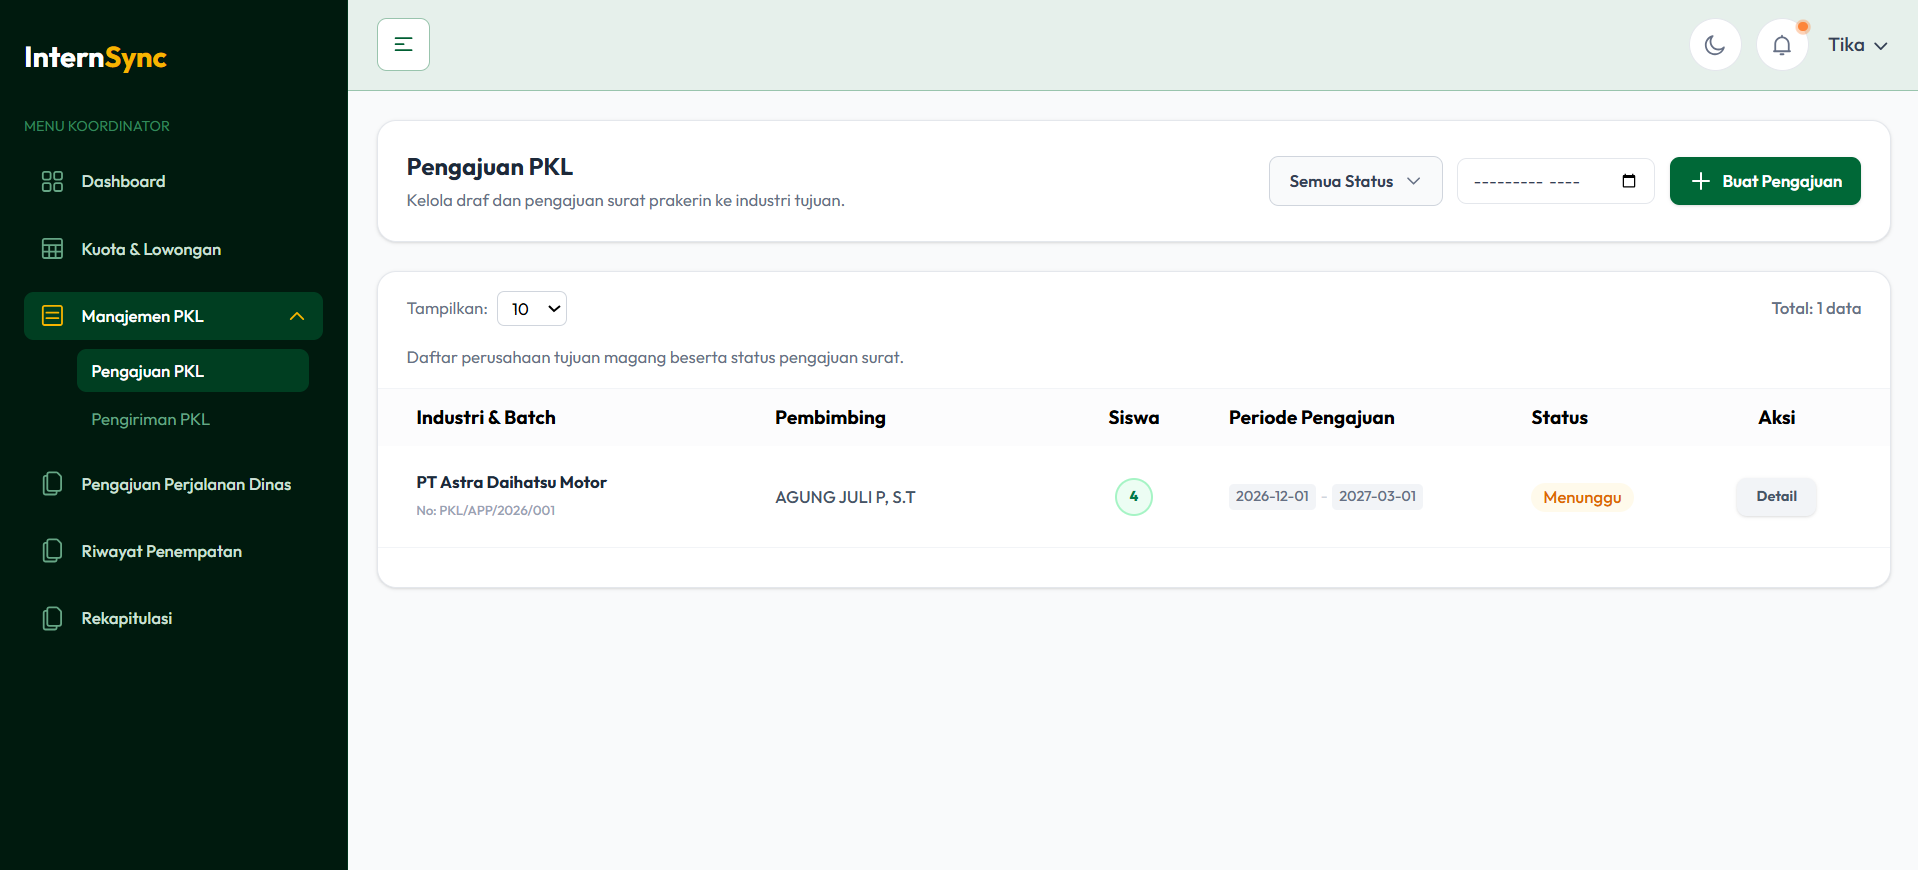
\includegraphics[width=14.00cm,height=0.78\textheight,keepaspectratio]{gambar/gambar-3-17.png}
\caption{Antarmuka Manajemen Pengajuan PKL (Koordinator)}\label{fig:3.17}
\end{figure}

Halaman ini merupakan antarmuka manajemen dokumen pengajuan penempatan PKL yang dikelola oleh Koordinator PKL pada submenu Pengajuan PKL. Komponen utama menampilkan \textit{data table} daftar permohonan penempatan yang telah disusun berdasarkan hasil seleksi lowongan, memuat atribut nama Industri dan Batch (beserta nomor registrasi dokumen \texttt{PKL/APP/...}), nama Guru Pembimbing yang ditugaskan, jumlah siswa dalam \textit{batch}, periode pengajuan magang, serta \textit{badge} status persetujuan (Menunggu, Disetujui, atau Ditolak). Halaman ini dilengkapi filter status dan periode tanggal, tombol Detail untuk meninjau rincian nominatif siswa, serta tombol + Buat Pengajuan di sudut kanan atas untuk membuka formulir pengajuan penempatan yang diteruskan kepada Waka Hubin.

\begin{figure}[H]
\centering
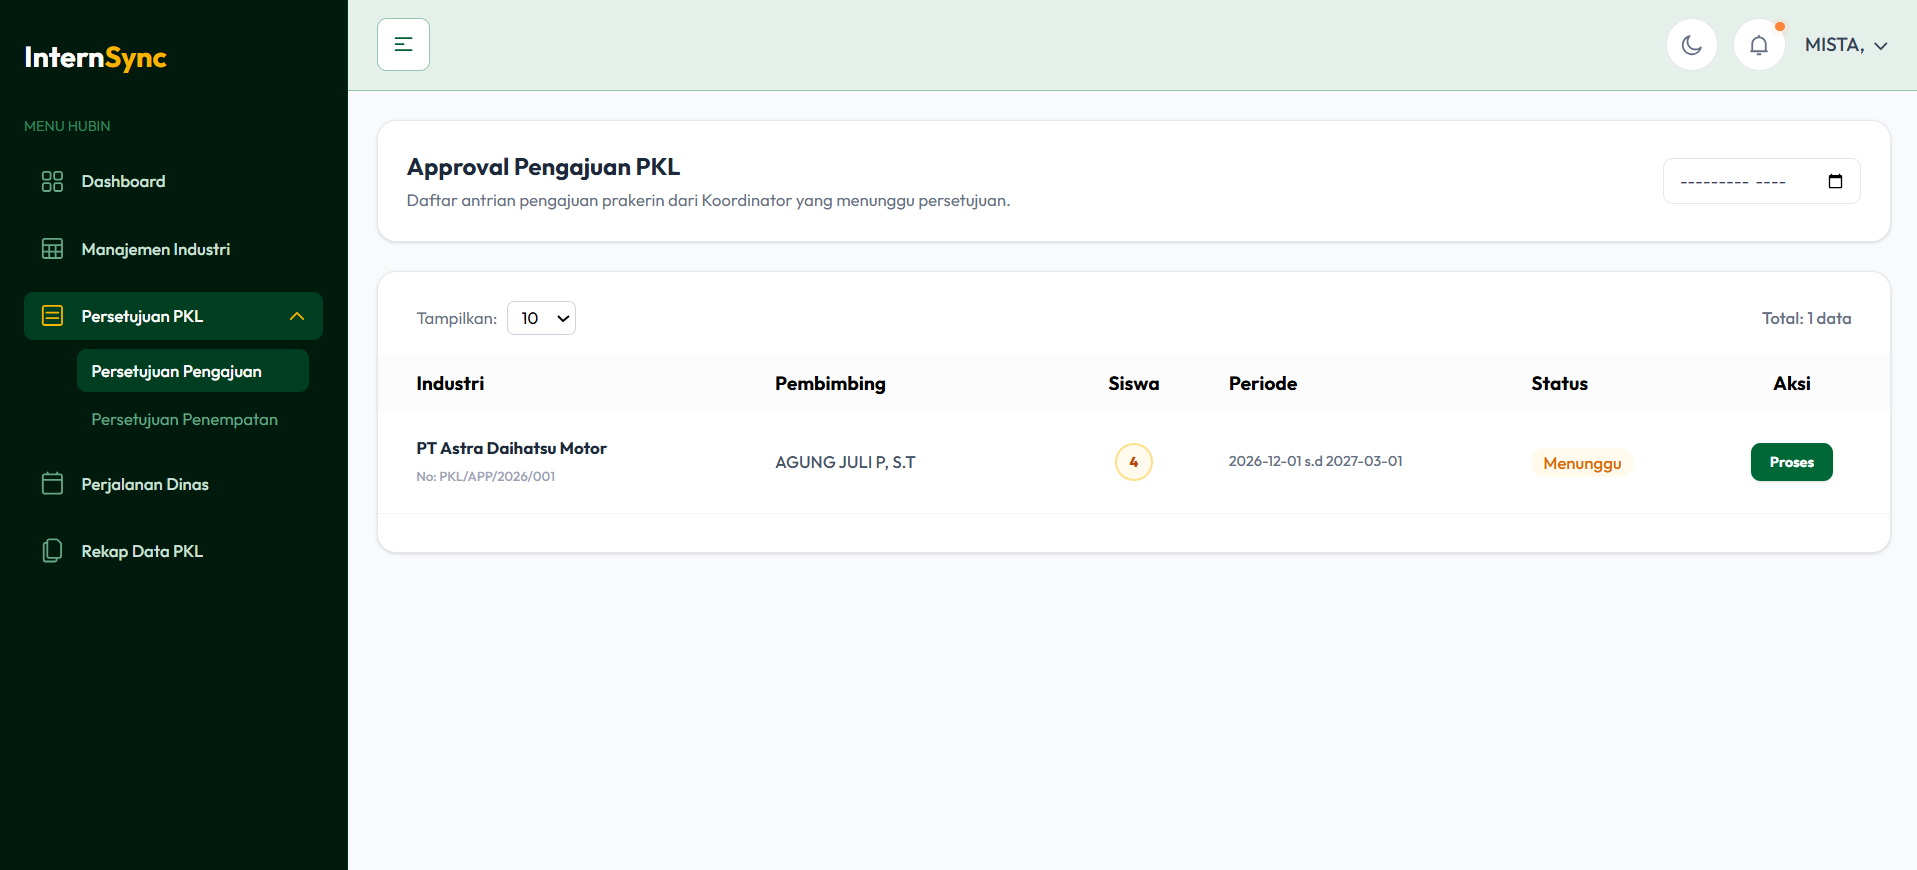
\includegraphics[width=14.00cm,height=0.78\textheight,keepaspectratio]{gambar/gambar-3-18.png}
\caption{Antarmuka Evaluasi dan Persetujuan Pengajuan PKL (Hubin)}\label{fig:3.18}
\end{figure}

Antarmuka ini berfungsi sebagai halaman antrean persetujuan (\textit{approval queue}) dokumen pengajuan penempatan PKL bagi Waka Hubin pada submenu Persetujuan Pengajuan. Halaman ini menyajikan \textit{data table} seluruh pengajuan masuk dari Koordinator PKL yang berstatus Menunggu, mencakup informasi perusahaan tujuan beserta nomor surat pengajuan, nama guru pembimbing pendamping, jumlah siswa peserta, serta rentang periode pelaksanaan yang diusulkan. Pada kolom aksi tersedia tombol Proses untuk membuka rincian dokumen dan memberikan keputusan persetujuan, yang otomatis menerbitkan Surat Pengantar PKL berformat PDF, atau penolakan disertai alasan revisi.

\begin{figure}[H]
\centering
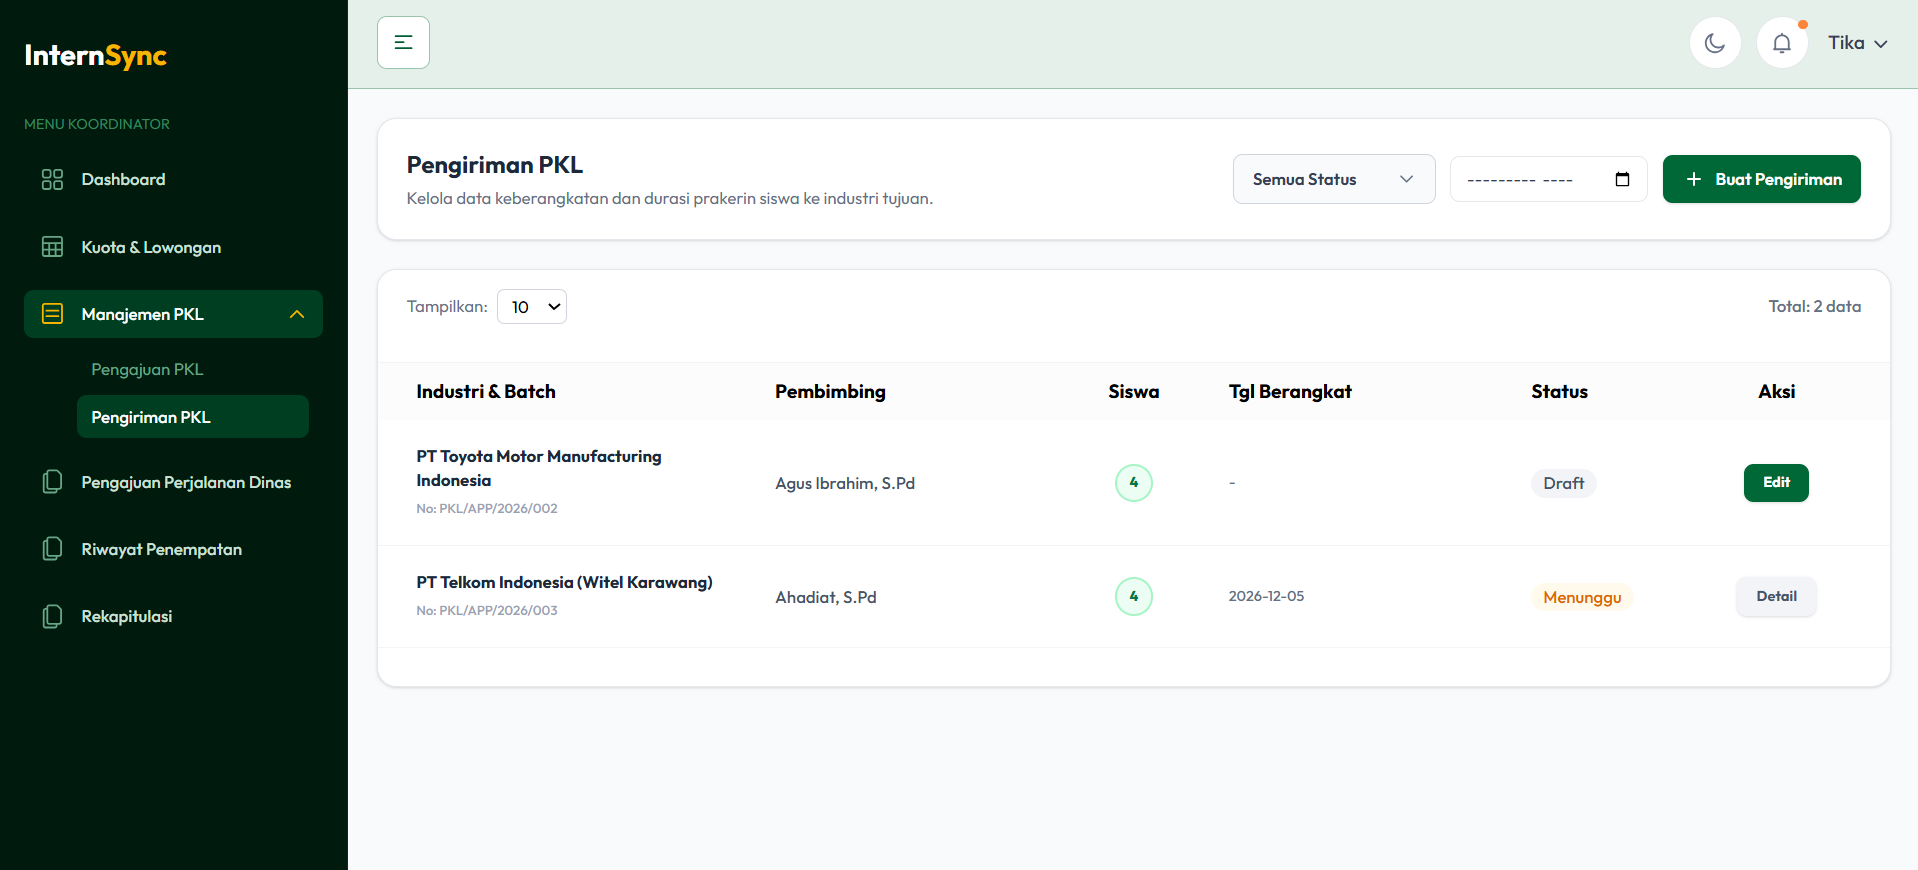
\includegraphics[width=14.00cm,height=0.78\textheight,keepaspectratio]{gambar/gambar-3-19.png}
\caption{Antarmuka Proses Pengiriman dan Penetapan Durasi PKL (Koordinator)}\label{fig:3.19}
\end{figure}

Halaman ini merupakan tindak lanjut pada submenu Pengiriman PKL setelah dokumen pengajuan awal disetujui Waka Hubin, yang berfokus pada pengelolaan jadwal keberangkatan siswa ke industri. Antarmuka menyajikan \textit{data table} daftar pengiriman per \textit{batch} industri beserta nama guru pembimbing, jumlah siswa, tanggal keberangkatan definitif, dan \textit{badge} status pengiriman (Draft atau Menunggu). Koordinator dapat menekan tombol + Buat Pengiriman atau Edit pada baris berstatus Draft untuk menetapkan tanggal mulai dan durasi PKL (3 atau 6 bulan), atau menekan Detail untuk memantau pengiriman yang menunggu \textit{clearance} akhir Hubin.

\begin{figure}[H]
\centering
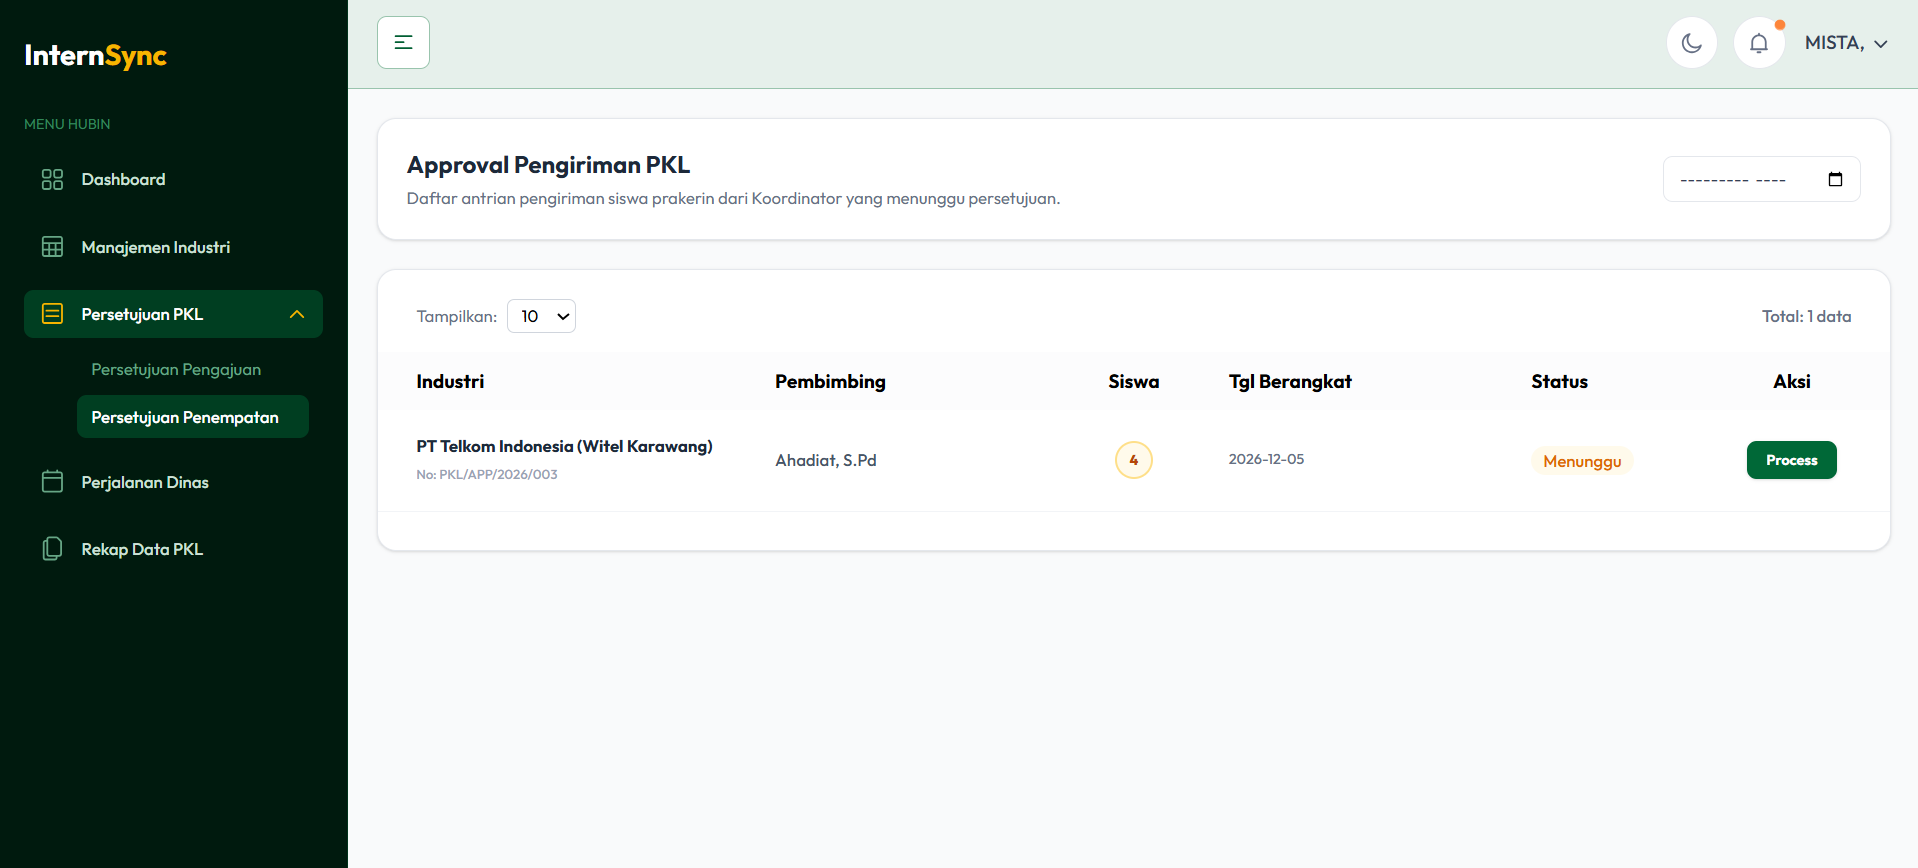
\includegraphics[width=14.00cm,height=0.78\textheight,keepaspectratio]{gambar/gambar-3-20.png}
\caption{Antarmuka Final Clearance dan Persetujuan Penempatan PKL (Hubin)}\label{fig:3.20}
\end{figure}

Antarmuka ini merepresentasikan tahap validasi keberangkatan akhir (\textit{final clearance}) oleh Waka Hubin pada submenu Persetujuan Penempatan sebelum siswa resmi berstatus aktif melaksanakan PKL di industri. Halaman ini menampilkan \textit{data table} antrean pengiriman siswa dari Koordinator PKL yang memuat informasi industri tujuan dan nomor dokumen, guru pembimbing, jumlah siswa, tanggal keberangkatan, serta status Menunggu. Melalui tombol Process, Waka Hubin dapat meninjau rincian final dan mengesahkan keberangkatan tersebut. Pengesahan menjadi pemicu sistemik yang mengubah status siswa menjadi aktif pada tabel \texttt{tr\_internships} serta membuka akses ke modul operasional harian (\textit{logbook} dan perizinan).

\subsubsection{Fase Pelaksanaan PKL (Monitoring, Logbook, Perizinan, dan Kunjungan)}

Fase ini memfasilitasi aktivitas operasional harian selama masa magang berlangsung, mencakup pencatatan rekam aktivitas kerja siswa, tata kelola presensi dan perizinan, verifikasi berkala oleh guru pembimbing, serta pemantauan kunjungan supervisi ke industri.

\begin{figure}[H]
\centering
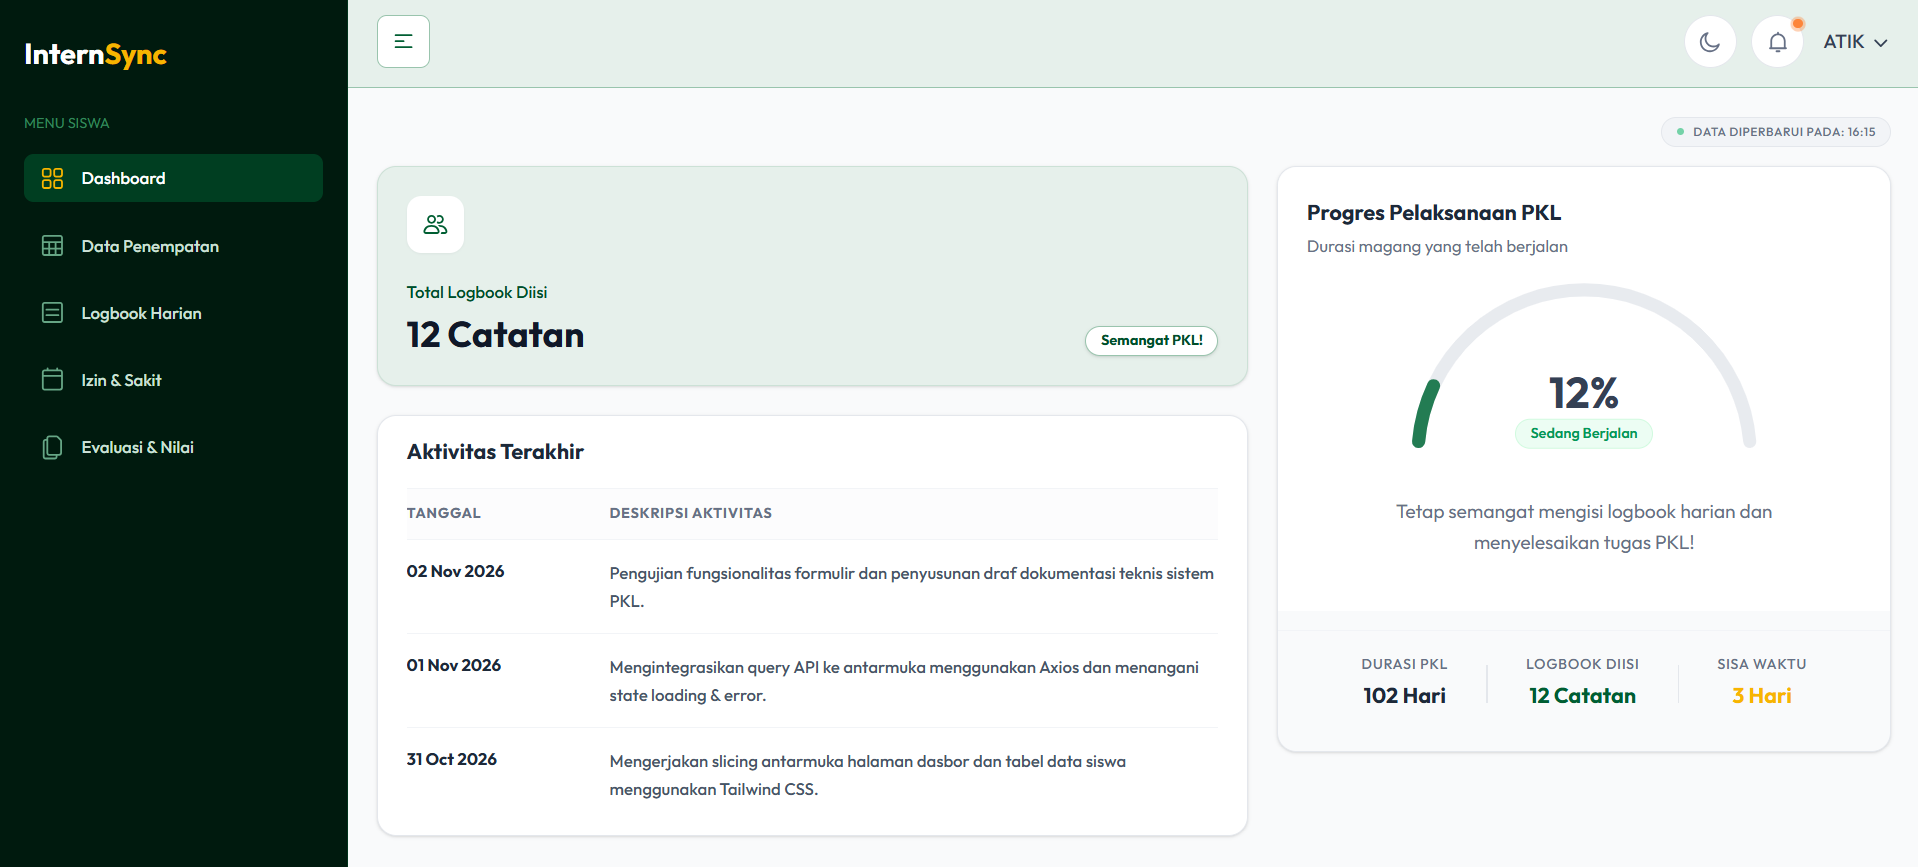
\includegraphics[width=14.00cm,height=0.78\textheight,keepaspectratio]{gambar/gambar-3-21.png}
\caption{Dasbor Antarmuka Siswa Prakerin (Tracking Progres PKL)}\label{fig:3.21}
\end{figure}

Antarmuka dasbor siswa berfungsi sebagai pusat kendali dan pemantauan informasi personal siswa selama menjalani masa PKL. Pada sisi kiri atas terdapat kartu ringkasan kuantitatif yang menampilkan metrik Total Logbook Diisi beserta lencana motivasi pelaksanaan. Di bawahnya tersaji tabel linimasa Aktivitas Terakhir yang merangkum tanggal dan deskripsi kegiatan \textit{logbook} terbaru. Pada sisi kanan, dasbor menampilkan \textit{gauge chart} (grafik setengah lingkaran progresif) pada panel Progres Pelaksanaan PKL yang menghitung persentase waktu magang yang telah ditempuh beserta total durasi PKL (hari), jumlah \textit{logbook} diisi, dan sisa waktu pelaksanaan.

\begin{figure}[H]
\centering
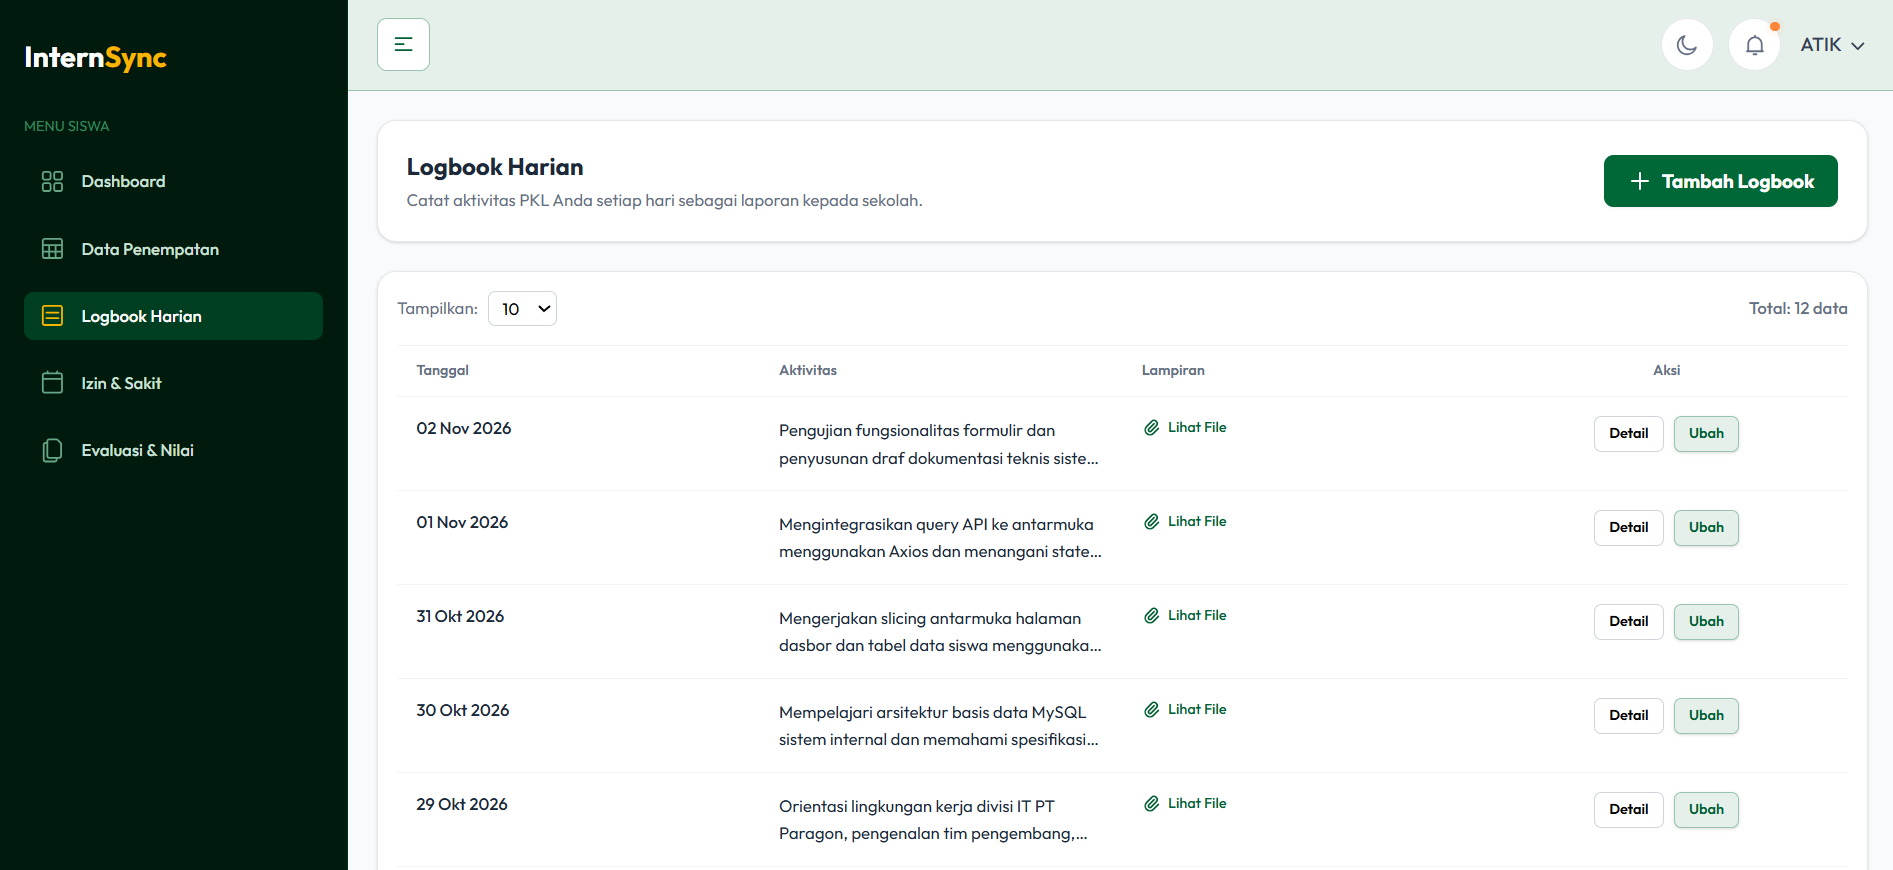
\includegraphics[width=14.00cm,height=0.78\textheight,keepaspectratio]{gambar/gambar-3-22.png}
\caption{Antarmuka Manajemen dan Pengisian Logbook Harian Siswa}\label{fig:3.22}
\end{figure}

Halaman ini merupakan instrumen utama siswa untuk mencatat rekam kegiatan operasional di industri secara mandiri (self-reporting logbook). Sistem menerapkan pendekatan pencatatan langsung tanpa melalui proses validasi berjenjang atau status persetujuan harian dari pembimbing, sehingga mempermudah siswa mendokumentasikan rutinitas kerja teknis di industri tanpa hambatan birokrasi harian. Komponen antarmuka terdiri atas data table rekapitulasi logbook per tanggal yang memuat kolom Tanggal pelaksanaan, Aktivitas pekerjaan, Lampiran bukti fisik, serta kolom Aksi. Tombol + Tambah Logbook membuka modal formulir pengisian tanggal kegiatan, uraian teknis pekerjaan yang dilakukan, serta tombol unggah berkas bukti fisik (foto kegiatan atau dokumen kerja). Formulir ini dilengkapi validasi otomatis berbasis kalender kerja yang membatasi pengisian hanya saat status PKL aktif, mendeteksi tanggal kerja yang belum diisi (mengecualikan hari libur dan izin/sakit), serta mencegah duplikasi pencatatan pada tanggal yang sama. Pada kolom aksi, siswa dapat menekan tombol Detail untuk meninjau rincian catatan aktivitas atau tombol Ubah untuk melakukan pembaruan konten dan lampiran kegiatan secara fleksibel.

\begin{figure}[H]
\centering
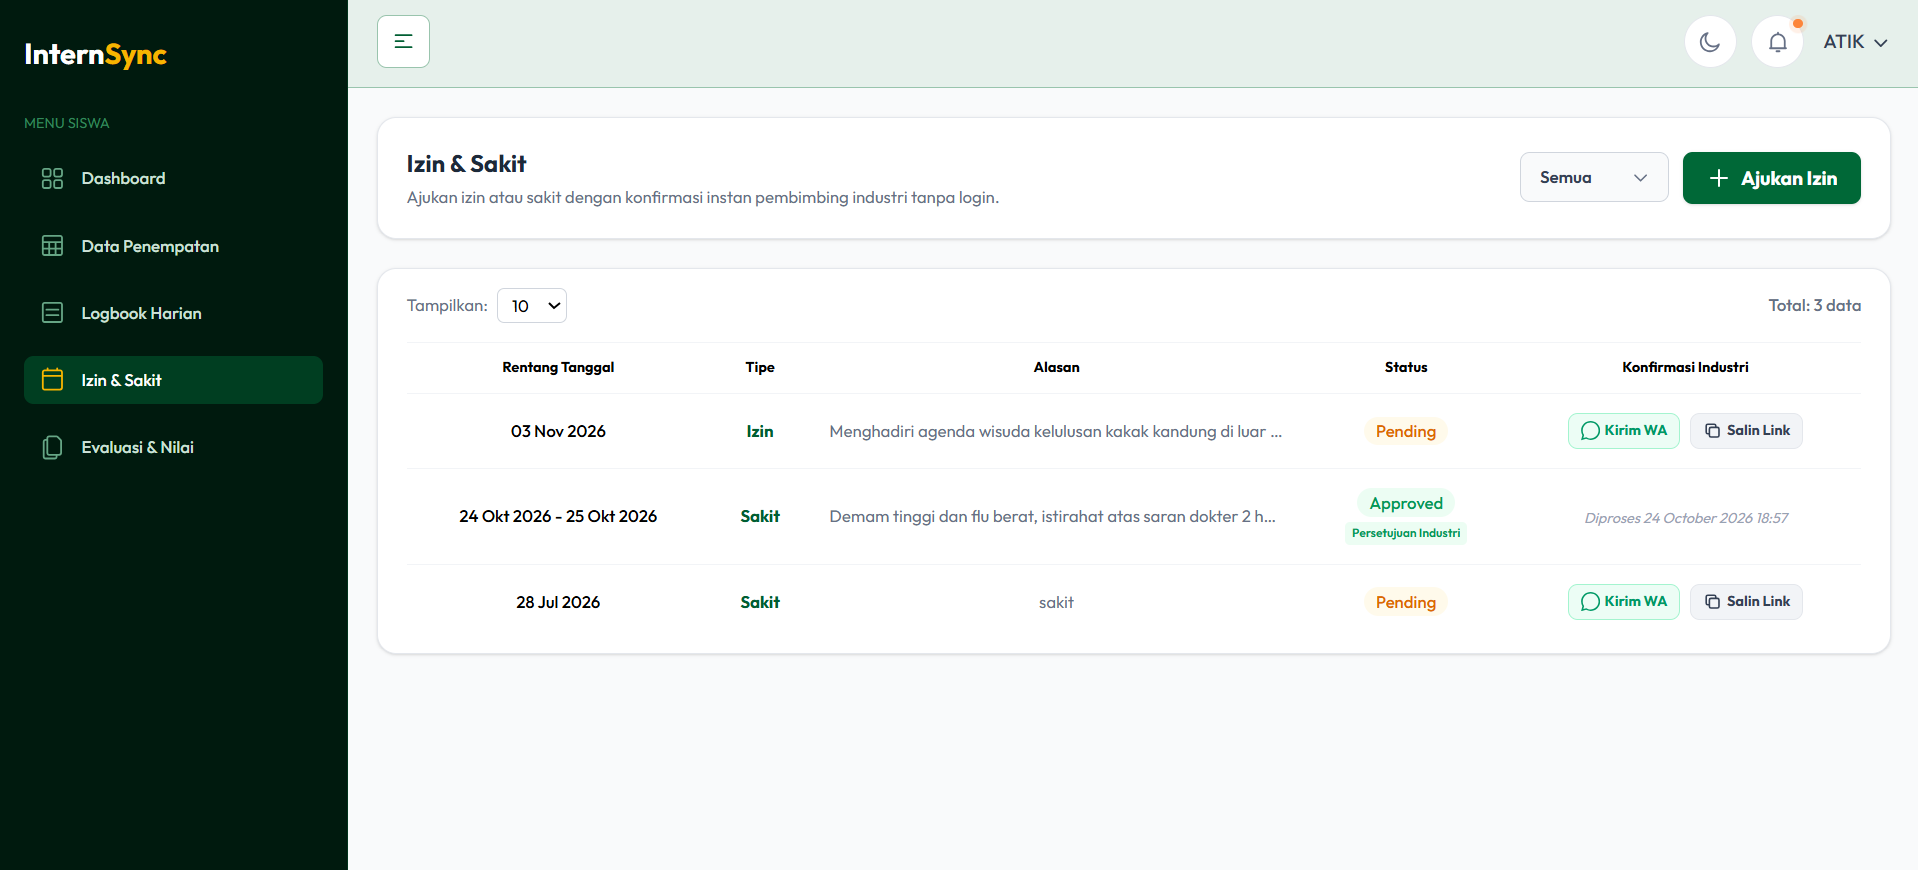
\includegraphics[width=14.00cm,height=0.78\textheight,keepaspectratio]{gambar/gambar-3-23.png}
\caption{Antarmuka Pengajuan Izin dan Sakit Siswa}\label{fig:3.23}
\end{figure}

Antarmuka ini menyediakan pencatatan ketidakhadiran siswa secara tertib dan transparan. Komponen utama menampilkan \textit{data table} riwayat permohonan izin/sakit dengan kolom Rentang Tanggal, Tipe permohonan (Izin atau Sakit), Alasan, \textit{badge} Status (Pending atau Approved beserta keterangan Persetujuan Industri), serta kolom Konfirmasi Industri. Siswa dapat menekan tombol + Ajukan Izin untuk menginput tanggal, alasan, dan mengunggah bukti sah (surat dokter atau surat orang tua). Untuk permohonan Pending, tersedia tombol Kirim WA dan Salin Link agar siswa dapat meneruskan tautan token persetujuan unik kepada Pembimbing Industri tanpa login.

\begin{figure}[H]
\centering
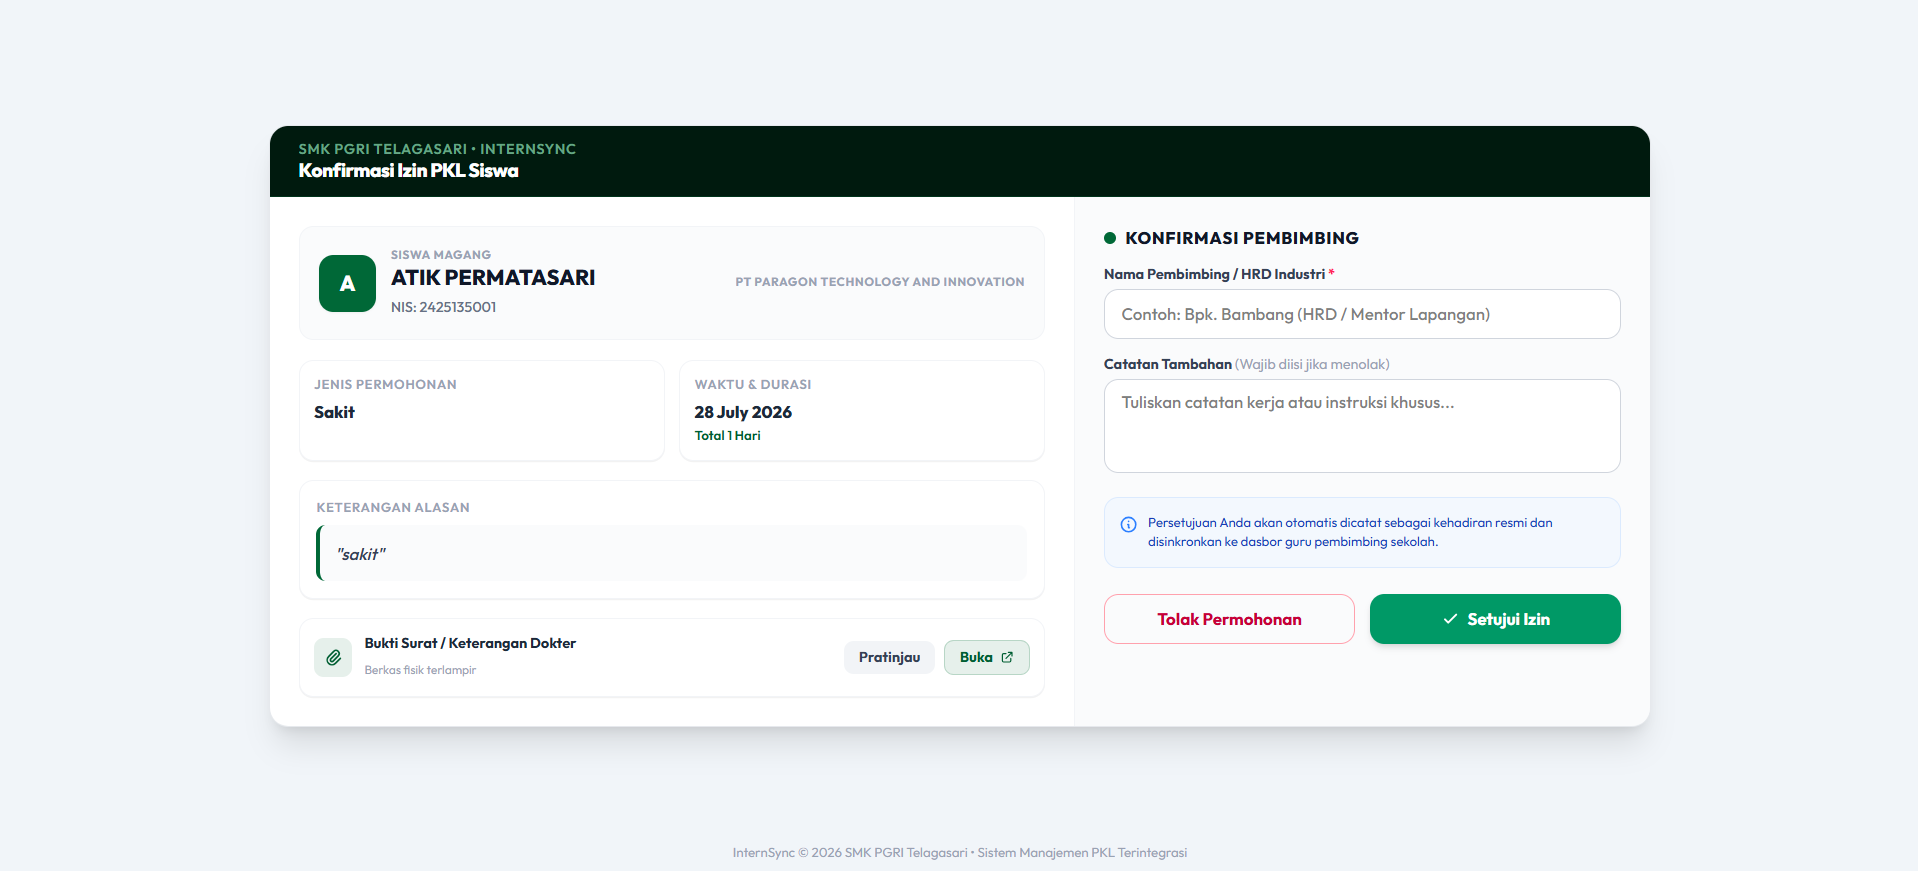
\includegraphics[width=14.00cm,height=0.78\textheight,keepaspectratio]{gambar/gambar-3-24.png}
\caption{Antarmuka Web Publik Persetujuan Izin Siswa via Tautan Token (Pembimbing Industri)}\label{fig:3.24}
\end{figure}

Halaman ini merupakan antarmuka publik berbasis rute token aman (/approval/izin/:token) yang digunakan Pembimbing Industri untuk memvalidasi permohonan izin siswa tanpa perlu login ke sistem. Halaman web responsif ini menampilkan rincian data siswa, tanggal ketidakhadiran, alasan, serta pratinjau dokumen surat dokter pendukung. Pembimbing Industri dapat menekan tombol Setujui Izin atau Tolak Izin. Sistem juga menerapkan mekanisme fallback 24 jam: apabila Pembimbing Industri belum merespons dalam kurun waktu tersebut, wewenang verifikasi izin dialihkan ke Guru Pembimbing Sekolah guna mencegah stagnasi data presensi.

\begin{figure}[H]
\centering
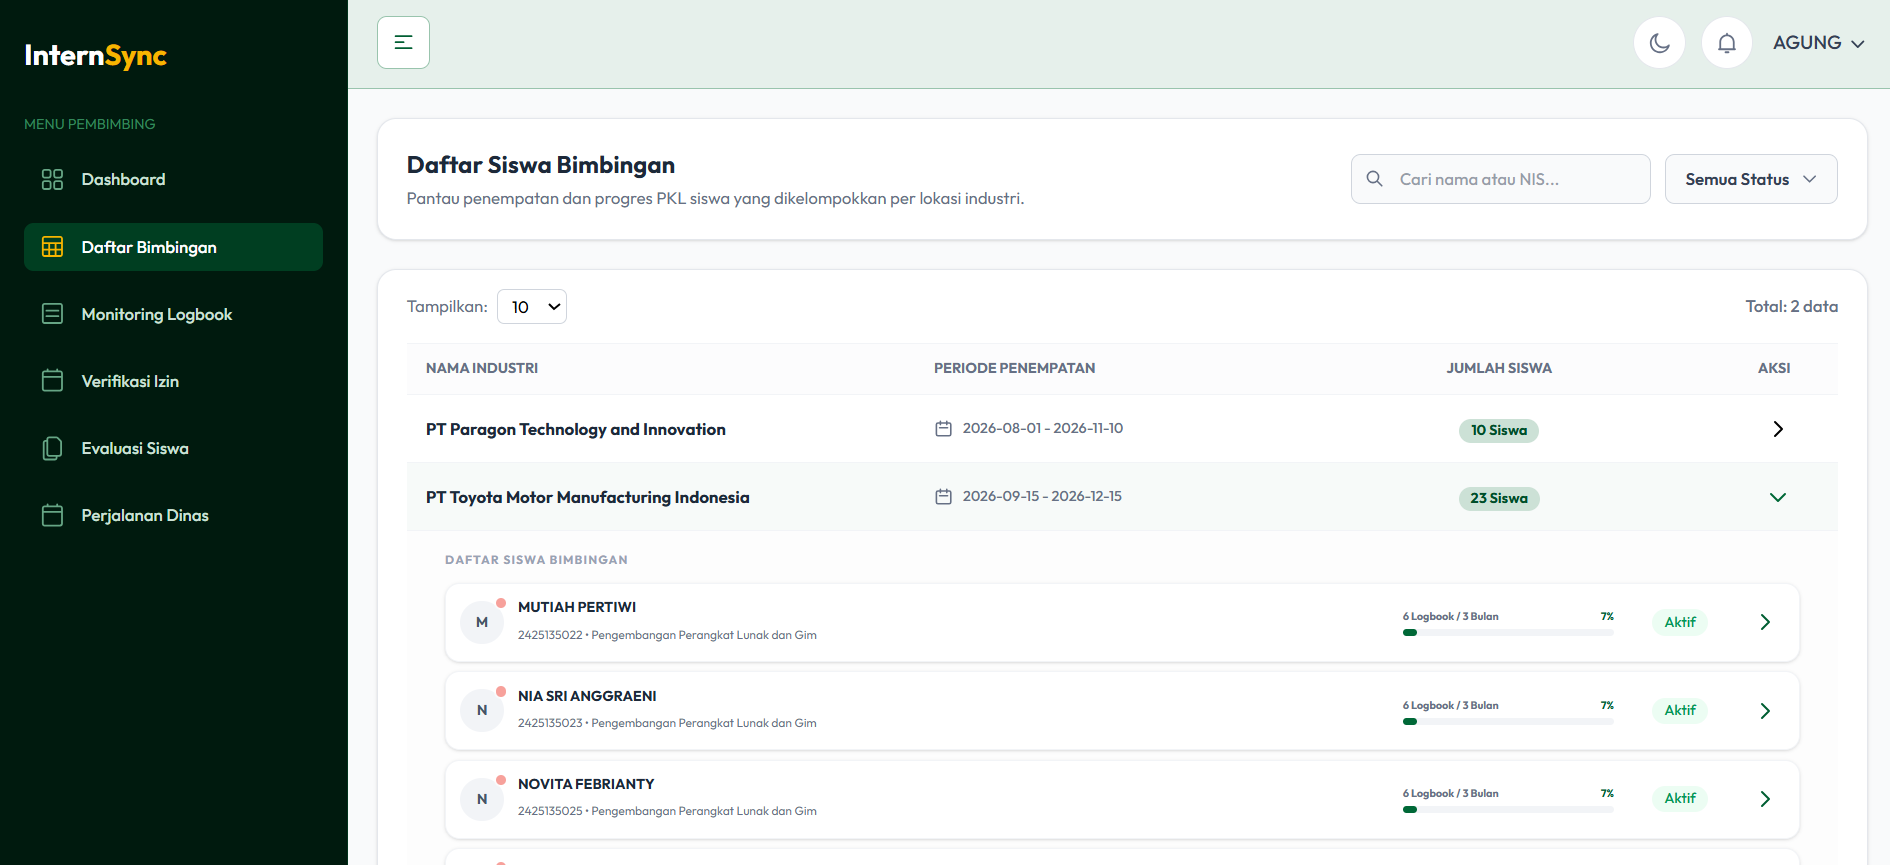
\includegraphics[width=14.00cm,height=0.78\textheight,keepaspectratio]{gambar/gambar-3-25.png}
\caption{Antarmuka Daftar Siswa Bimbingan (Guru Pembimbing)}\label{fig:3.25}
\end{figure}

Halaman pembimbing ini menyajikan informasi pengawasan siswa yang berada di bawah tanggung jawab supervisinya. Antarmuka menampilkan tabel hierarkis yang mengelompokkan siswa berdasarkan industri tempat mereka ditempatkan. Setiap baris data siswa memuat indikator progres pengisian logbook, status operasional, serta tombol aksi untuk meninjau detail logbook, riwayat perizinan, dan agenda kunjungan.

\begin{figure}[H]
\centering
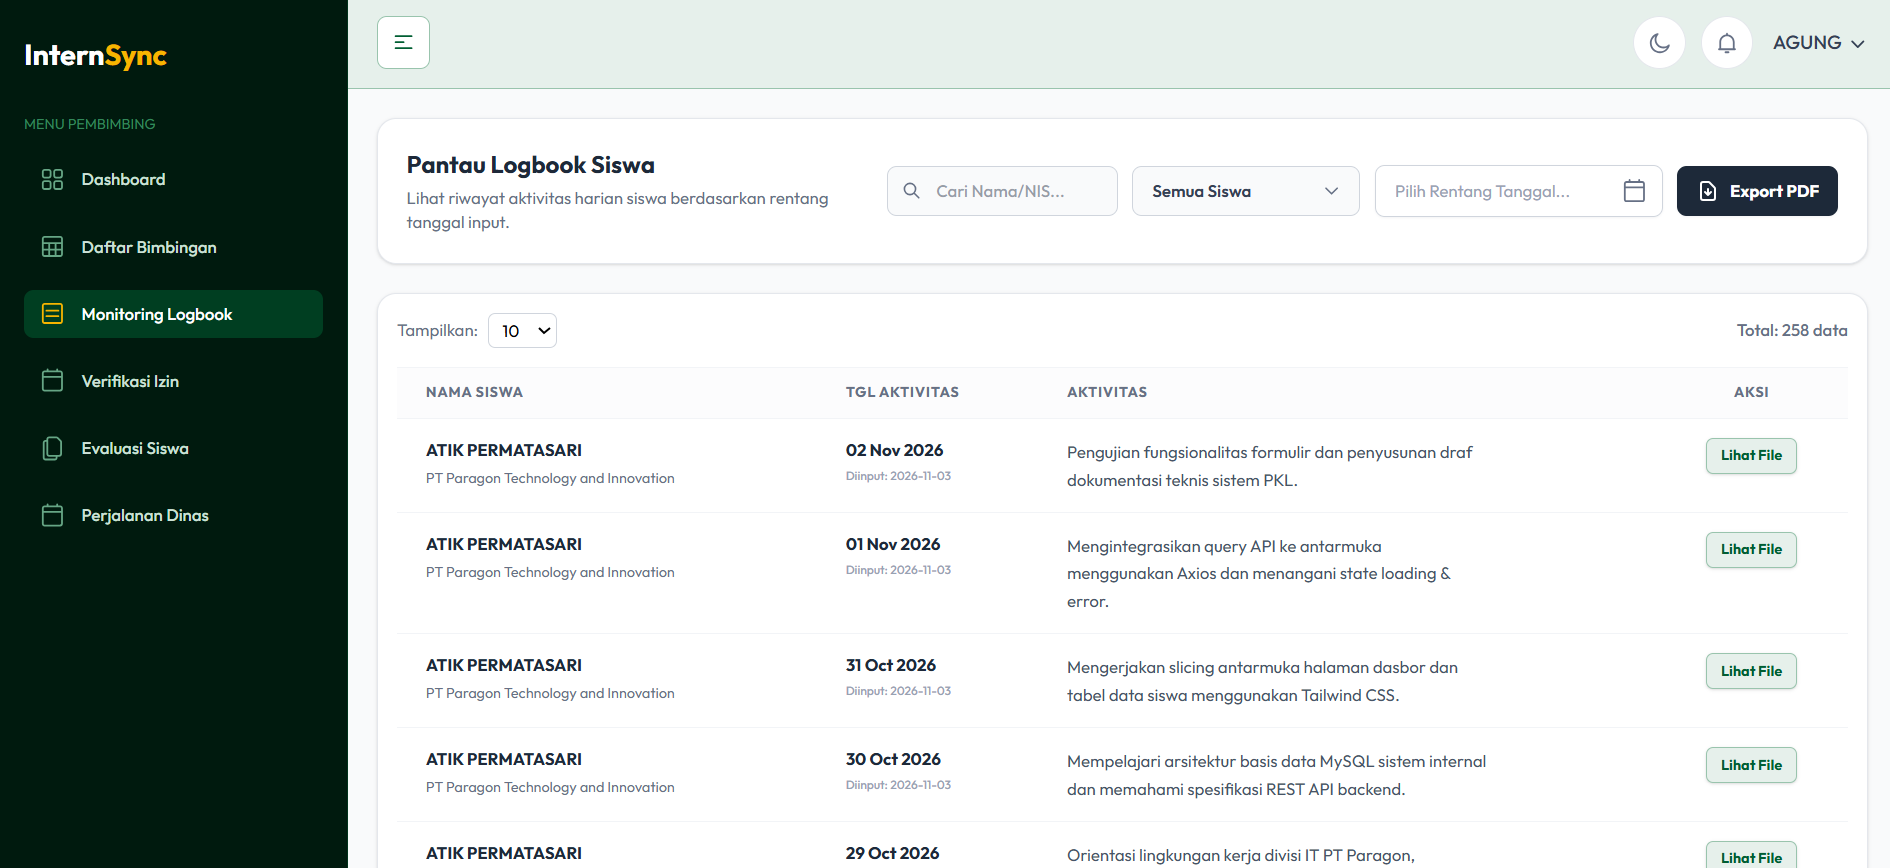
\includegraphics[width=14.00cm,height=0.78\textheight,keepaspectratio]{gambar/gambar-3-26.png}
\caption{Antarmuka Monitoring Logbook Siswa (Guru Pembimbing)}\label{fig:3.26}
\end{figure}

Antarmuka ini merupakan instrumen supervisi, pemantauan, dan kendali mutu kegiatan bimbingan magang siswa oleh guru pembimbing sekolah. Komponen utama terdiri atas data table rekapitulasi jurnal harian dengan fungsionalitas penyaringan tingkat lanjut (pencarian nama/NIS siswa, filter dropdown daftar siswa bimbingan, dan rentang tanggal kegiatan). Guru pembimbing dapat memantau kedisiplinan dan kontinuitas pengisian jurnal kerja, meninjau deskripsi aktivitas pekerjaan teknis beserta kendala yang dihadapi siswa, serta membuka berkas foto lampiran bukti fisik kegiatan secara langsung melalui modal peninjau berkas (attachment modal). Berbeda dengan pendekatan konvensional yang membebani pembimbing dengan antrean persetujuan manual per entitas baris setiap hari, sistem InternSync menerapkan mekanisme self-reporting terstruktur di mana seluruh catatan logbook yang diunggah siswa langsung terarsipkan secara transparan. Pada bagian atas tabel, halaman ini dilengkapi tombol Ekspor Logbook (PDF) yang mengompilasi seluruh catatan harian siswa secara otomatis menjadi bundel laporan resmi yang tervalidasi tanda tangan digital QR Code sebagai berkas portofolio pendukung evaluasi dan pertimbangan rubrik penilaian akhir PKL.

\begin{figure}[H]
\centering
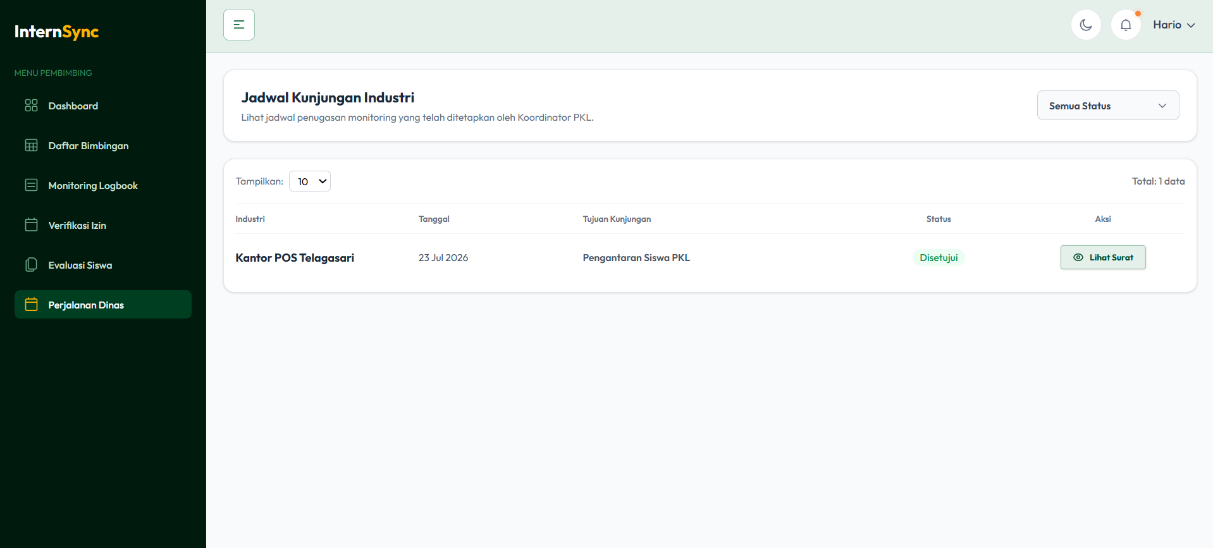
\includegraphics[width=14.00cm,height=0.78\textheight,keepaspectratio]{gambar/gambar-3-27.png}
\caption{Antarmuka Monitoring Kunjungan Industri dan Surat Tugas SPPD (Guru Pembimbing)}\label{fig:3.27}
\end{figure}

Antarmuka pada menu Perjalanan Dinas ini memfasilitasi Guru Pembimbing dalam memantau jadwal penugasan kunjungan supervisi ke industri mitra yang telah ditetapkan oleh Koordinator PKL. Komponen utama menampilkan \textit{data table} daftar penugasan kunjungan yang memuat nama industri, tanggal pelaksanaan, tujuan kunjungan (seperti pengantaran Siswa PKL), serta \textit{badge} status persetujuan (Disetujui). Pada kolom aksi tersedia tombol Lihat Surat untuk melihat dan mengunduh dokumen Surat Perintah Perjalanan Dinas (SPPD) resmi berformat PDF.

\subsubsection{Fase Pasca-PKL (Evaluasi Kinerja, Rubrik Penilaian Akhir, dan Rekapitulasi)}

Fase penutup ini mencakup alur finalisasi nilai hasil pelaksanaan PKL yang mengintegrasikan penilaian kinerja industri dan evaluasi laporan sekolah berdasarkan rubrik baku, publikasi hasil nilai kepada siswa, serta ekstraksi laporan rekapitulasi akhir sekolah.

\begin{figure}[H]
\centering
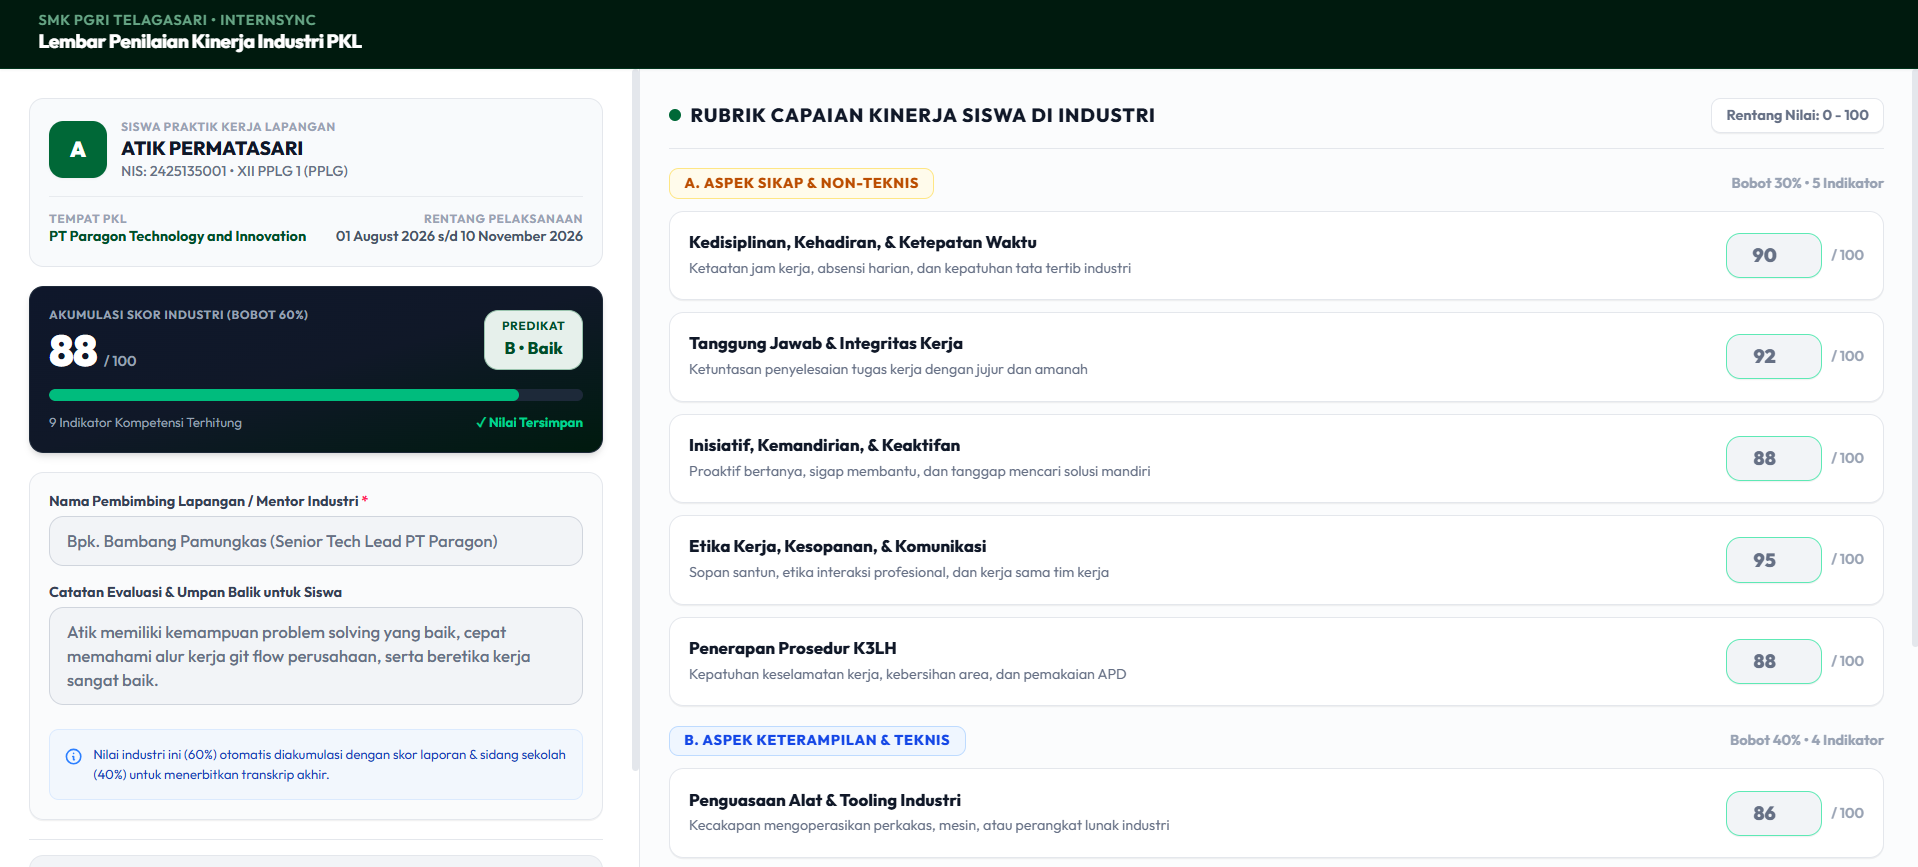
\includegraphics[width=14.00cm,height=0.78\textheight,keepaspectratio]{gambar/gambar-3-28.png}
\caption{Antarmuka Web Publik Penilaian Rubrik Kinerja Industri 60\% (Pembimbing Industri)}\label{fig:3.28}
\end{figure}

Antarmuka ini beroperasi pada rute publik berbasis token \url{/penilaian-industri/:token} yang memungkinkan Pembimbing Industri memberikan penilaian kinerja objektif kepada siswa bimbingannya tanpa autentikasi akun. Formulir menampilkan 9 indikator rubrik baku evaluasi magang SMK dalam dua kelompok: aspek sikap dan non-teknis (kedisiplinan dan kehadiran, tanggung jawab dan integritas kerja, inisiatif dan kemandirian, etika kerja dan komunikasi, serta penerapan K3LH) dan aspek keterampilan dan teknis (penguasaan peralatan dan tooling industri, kualitas dan presisi hasil pekerjaan, analisis dan pemecahan masalah, serta kecepatan dan ketuntasan tugas). Nilai diinputkan pada kolom numerik 0–100, dan sistem menampilkan akumulasi skor industri yang berkontribusi 60\% terhadap nilai akhir PKL siswa. Dua indikator lainnya, yaitu aspek akademik dan laporan, dinilai oleh Guru Pembimbing (Gambar 3.29).

\begin{figure}[H]
\centering
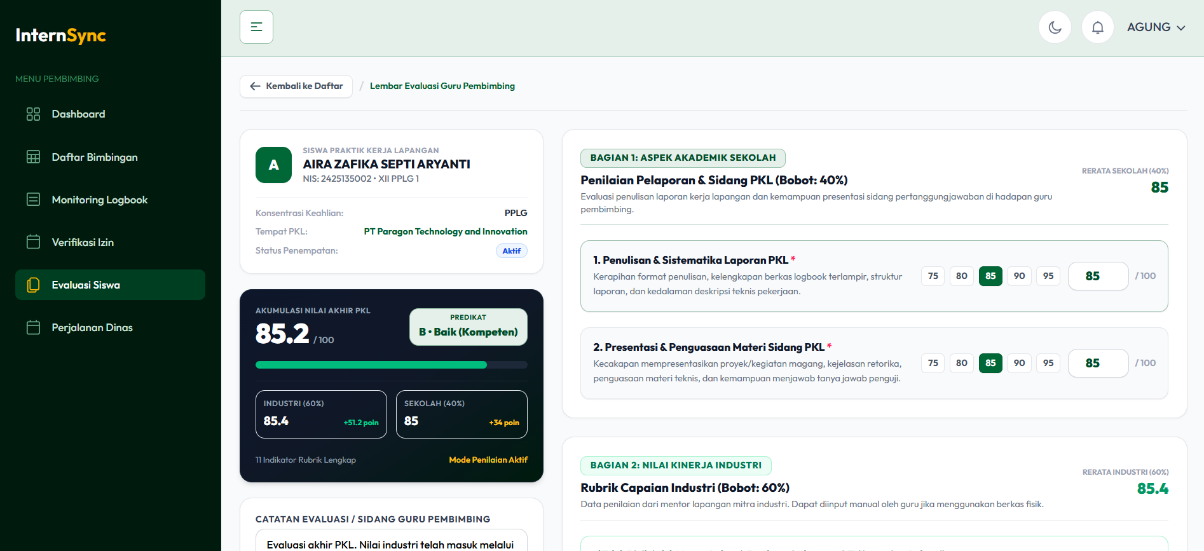
\includegraphics[width=13.89cm,height=0.78\textheight,keepaspectratio]{gambar/gambar-3-29.png}
\caption{Antarmuka Manajemen dan Input Penilaian Sekolah 40\% (Guru Pembimbing)}\label{fig:3.29}
\end{figure}

Halaman Lembar Evaluasi Guru Pembimbing ini digunakan untuk menginput nilai akademik sekolah sekaligus memfinalisasi nilai akhir PKL siswa bimbingan. Sisi kiri menampilkan kartu profil siswa (nama, NIS, kelas, konsentrasi keahlian, dan tempat PKL), kartu Akumulasi Nilai Akhir PKL yang menghitung skor gabungan secara \textit{real-time} beserta predikat kelulusan (misalnya \texttt{85.2 / 100 -- Predikat B Baik (Kompeten)}) dan kontribusi poin Industri 60\% versus Sekolah 40\%, serta kolom catatan evaluasi sidang. Sisi kanan menampilkan formulir Bagian 1: Aspek Akademik Sekolah (Bobot 40\%) untuk memberi skor melalui tombol cepat atau input angka 0--100 pada komponen Penulisan dan Sistematika Laporan PKL serta Presentasi dan Penguasaan Materi Sidang PKL, disertai ringkasan Bagian 2: Nilai Kinerja Industri (Bobot 60\%) dari pembimbing lapangan.

\begin{figure}[H]
\centering
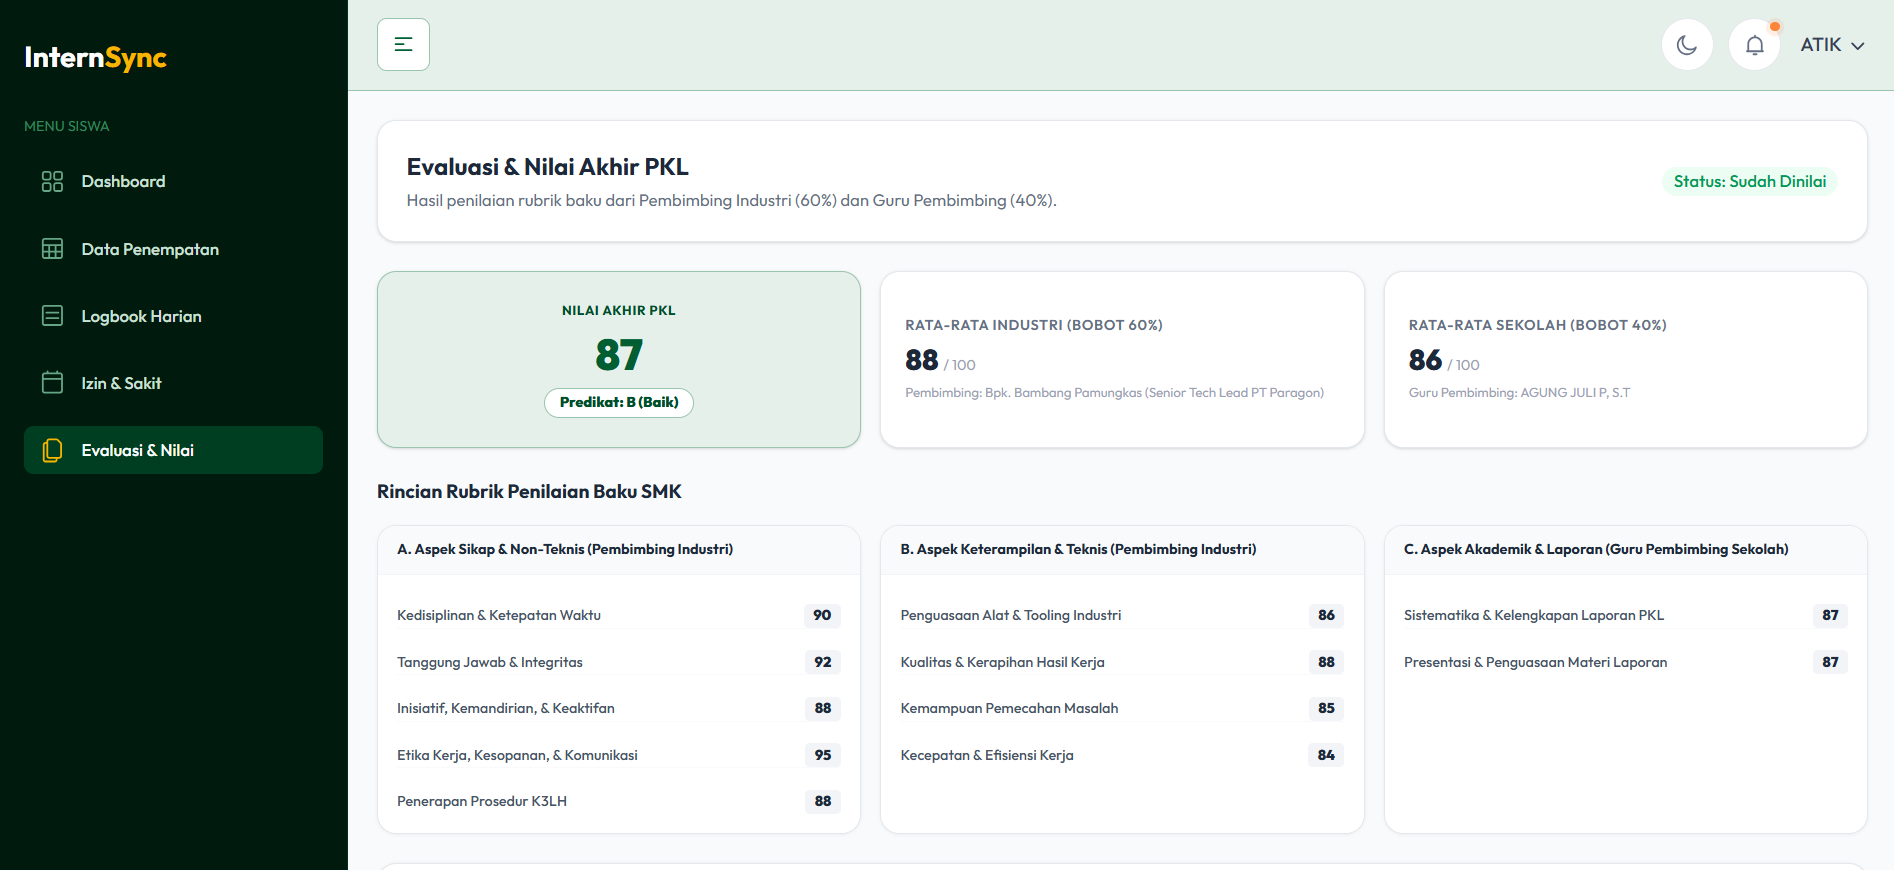
\includegraphics[width=14.00cm,height=0.78\textheight,keepaspectratio]{gambar/gambar-3-30.png}
\caption{Antarmuka Akses Hasil Evaluasi dan Lembar Nilai Akhir Siswa (Published)}\label{fig:3.30}
\end{figure}

Antarmuka pada menu Evaluasi \& Nilai ini menyajikan hasil akhir PKL setelah penilaian difinalisasi oleh Pembimbing Industri dan Guru Pembimbing Sekolah, ditandai dengan \textit{badge} Status: Sudah Dinilai. Bagian atas menampilkan kartu Nilai Akhir PKL beserta predikat, Rata-rata Industri (Bobot 60\%) beserta nama mentor lapangan, dan Rata-rata Sekolah (Bobot 40\%) beserta nama guru pembimbing. Di bagian bawah disajikan rincian skor 11 indikator dalam tiga kelompok: aspek sikap dan non-teknis (Pembimbing Industri), aspek keterampilan dan teknis (Pembimbing Industri), serta aspek akademik dan laporan (Guru Pembimbing Sekolah). Siswa dapat mengunduh lembar nilai resmi berformat PDF ber-QR Code untuk menjamin keaslian dokumen.

\begin{figure}[H]
\centering
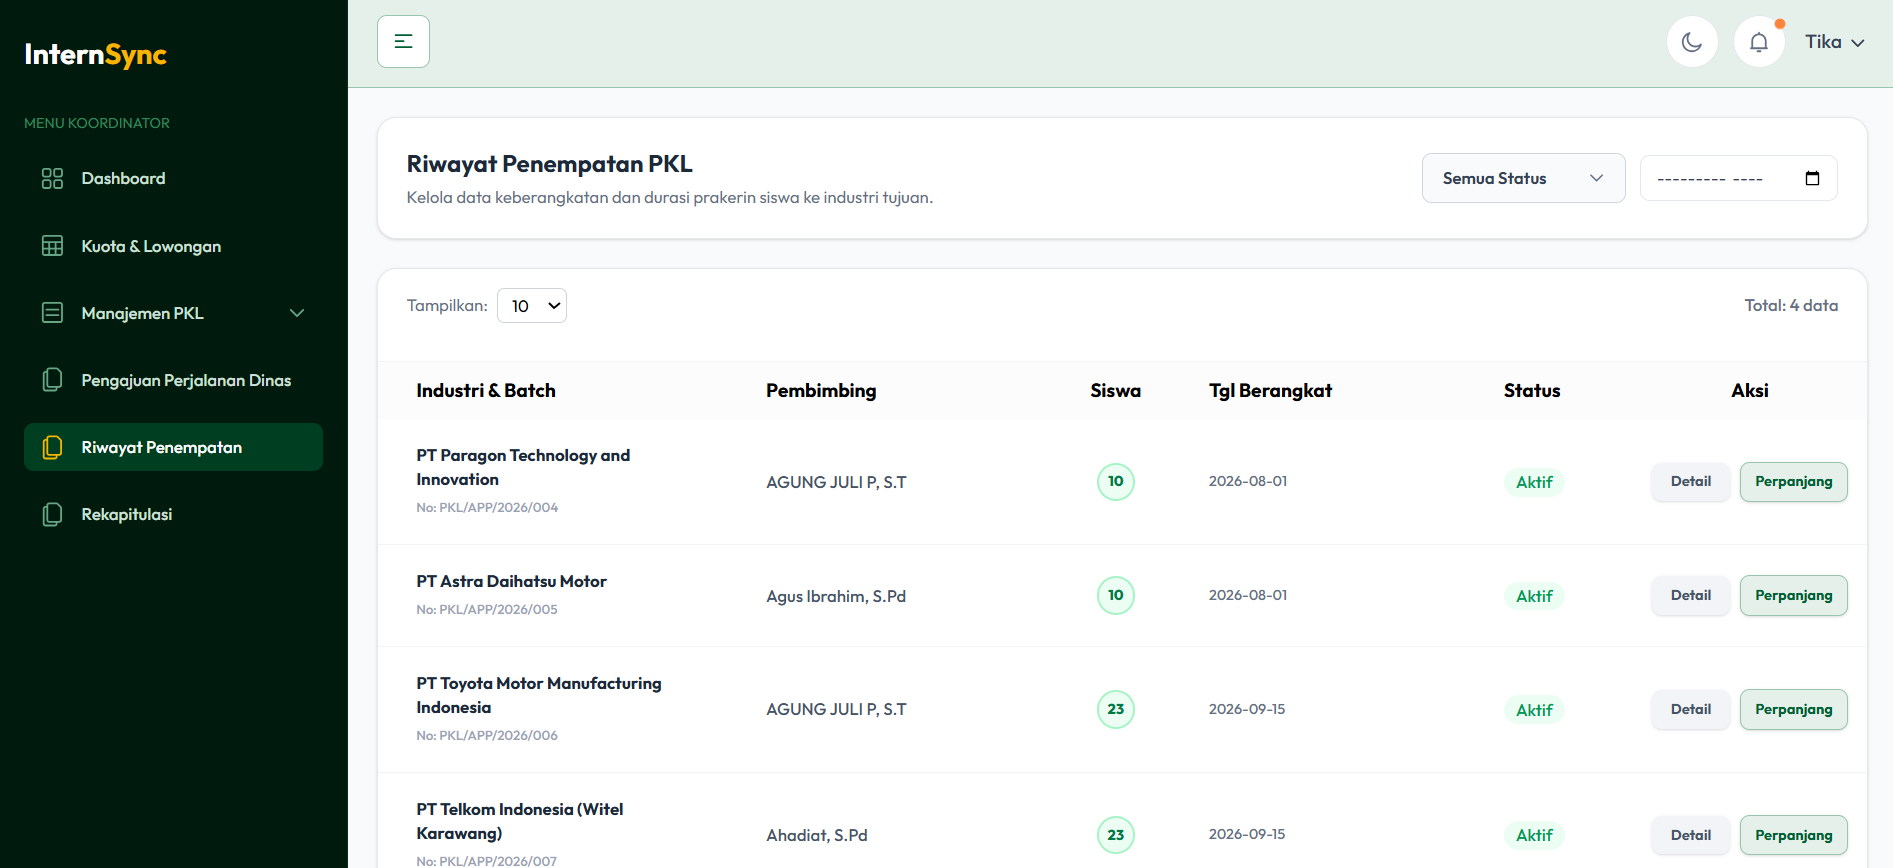
\includegraphics[width=14.00cm,height=0.78\textheight,keepaspectratio]{gambar/gambar-3-31.png}
\caption{Antarmuka Riwayat Penempatan dan Pengelolaan Durasi PKL (Koordinator)}\label{fig:3.31}
\end{figure}

Antarmuka ini berfungsi sebagai pusat pemantauan riwayat keberangkatan dan pengelolaan durasi penempatan PKL oleh Koordinator. Komponen utamanya berupa \textit{data table} yang merangkum pengiriman per kelompok (\textit{batch}) berdasarkan industri tujuan dan nomor dokumen pengajuan, guru pembimbing, jumlah siswa, tanggal keberangkatan, serta status pelaksanaan (Aktif/Selesai). Halaman ini dilengkapi filter status dan periode keberangkatan, serta tombol Detail untuk meninjau siswa dan Perpanjang untuk memperbarui masa PKL.

\section{RENCANA PENGEMBANGAN APLIKASI MOBILE (SISWA DAN GURU PEMBIMBING)}

Sebagai pengembangan lanjutan, aplikasi \textit{mobile} direncanakan untuk memfasilitasi mobilitas operasional harian di lapangan bagi peran Siswa dan Guru Pembimbing. Aplikasi ini direncanakan dibangun menggunakan framework Flutter (Dart), yang memungkinkan kompilasi lintas platform menggunakan satu basis kode yang efisien. Pada proyek akhir ini, fokus implementasi adalah aplikasi web, sedangkan aplikasi \textit{mobile} masih berada pada tahap perencanaan dan belum direalisasikan. Aplikasi \textit{mobile} tidak dirancang sebagai entitas independen, melainkan direncanakan beroperasi sebagai \textit{frontend} seluler yang terintegrasi langsung dengan \textit{backend} Laravel melalui arsitektur RESTful API yang sama dengan aplikasi web. Pendekatan ini lazim diterapkan pada pengembangan aplikasi \textit{mobile} berbasis Flutter yang mengandalkan REST API sebagai jembatan komunikasi data dengan \textit{backend}, sebagaimana diterapkan pada penelitian pengembangan aplikasi \textit{reimbursement} berbasis Android \cite{ref16}. Autentikasi berbasis token yang telah diimplementasikan melalui Laravel Sanctum pada aplikasi web juga sejalan dengan praktik umum penerapan \textit{Bearer Token}/JSON Web Token (JWT) pada arsitektur REST API untuk menjamin keamanan sesi pengguna \cite{ref17}, dan dapat digunakan kembali oleh aplikasi \textit{mobile}.

Pendekatan \textit{client-server} berbasis REST API terpusat ini diharapkan menjaga konsistensi dan integritas data antara platform \textit{web} dan \textit{mobile}. Fungsionalitas aplikasi \textit{mobile} direncanakan difokuskan pada kepraktisan pelaporan harian siswa di lokasi magang serta kemudahan pengawasan Guru Pembimbing di lapangan dengan rencana fitur sebagai berikut:

\begin{enumerate}[label=\alph*.]
\item \textbf{Autentikasi Terpusat dan Keamanan Sesi}
\par\noindent Sistem login direncanakan menggunakan kredensial (Email/NIP/NIS dan kata sandi) yang sama dengan versi \textit{web}. Autentikasi direncanakan memanfaatkan \textit{Bearer Token} berbasis REST (Laravel Sanctum) untuk mengelola sesi secara aman dan mengarahkan tampilan aplikasi sesuai peran pengguna (Siswa atau Guru Pembimbing) tanpa perlu login berulang kali.
\item \textbf{Dasbor Ringkas (\textit{Executive Summary})}
\par\noindent Dasbor direncanakan menyajikan metrik esensial sesuai peran pengguna. Bagi siswa, dasbor menampilkan persentase progres durasi PKL dan total catatan \textit{logbook} harian yang telah diisi. Bagi Guru Pembimbing, dasbor menampilkan total siswa bimbingan aktif, permohonan izin \textit{fallback} yang perlu ditinjau, serta jadwal kunjungan terdekat.
\item \textbf{Pencatatan dan Pemantauan Logbook Harian}
\par\noindent Siswa direncanakan dapat mencatat aktivitas kerja harian secara mandiri (\textit{self-reporting}) dan mengunggah foto dokumentasi kegiatan langsung dari kamera ponsel saat berada di lokasi industri. Guru Pembimbing direncanakan dapat memantau riwayat aktivitas harian dan memeriksa lampiran bukti kegiatan siswa bimbingannya melalui ponsel.
\item \textbf{Pengajuan Izin/Sakit dan Mekanisme Fallback Presensi}
\par\noindent Siswa direncanakan dapat mengajukan permohonan izin atau sakit beserta unggahan foto surat keterangan dokter dan membagikan tautan token konfirmasi kepada Pembimbing Industri melalui WhatsApp. Guru Pembimbing direncanakan dapat memverifikasi izin melalui mekanisme \textit{fallback} apabila pihak industri belum merespons dalam waktu 24 jam.
\item \textbf{Pemantauan Progres dan Evaluasi Lapangan}
\par\noindent Aplikasi direncanakan menampilkan daftar siswa di bawah supervisi Guru Pembimbing beserta lokasi industri dan indikator penyelesaian durasi PKL, serta memfasilitasi input nilai pembimbingan sekolah (40\%) dan peninjauan hasil evaluasi akhir saat supervisi kunjungan industri.
\end{enumerate}

Desain antarmuka (UI/UX) aplikasi \textit{mobile} direncanakan berfokus pada kemudahan navigasi dan efisiensi interaksi (\textit{user-friendly}), dengan menghindari elemen visual berlebihan agar aplikasi tetap ringan dijalankan pada berbagai spesifikasi perangkat ponsel siswa maupun tenaga pendidik. Hingga aplikasi \textit{mobile} terealisasi, kebutuhan mobilitas tersebut dilayani oleh antarmuka web responsif yang telah diuji pada resolusi ponsel (subbab 4.7).

\section{RENCANA PENGUJIAN SISTEM}

Untuk menjamin keandalan, stabilitas, dan kesesuaian sistem InternSync dengan kebutuhan pengguna di SMK PGRI Telagasari, pengujian perangkat lunak akan dilakukan menggunakan metode Black Box Testing. Fokus pengujian murni berada pada validasi fungsionalitas input dan output dari perspektif pengguna akhir, tanpa perlu menganalisis atau membongkar struktur kode internal (source code) \cite{ref18}.

Metode Black Box Testing dipilih karena memungkinkan pengujian dilakukan murni dari sudut pandang pengguna akhir tanpa memerlukan pengetahuan teknis terhadap struktur kode program \cite{ref19}. Salah satu teknik yang umum digunakan dalam pendekatan ini adalah analisis nilai batas (boundary value analysis), yang efektif untuk menguji validitas input pada kondisi-kondisi ekstrem seperti batas ukuran file atau format data numerik \cite{ref20}.

Skenario pengujian komprehensif ini dirancang untuk mencakup beberapa parameter operasional utama:

\begin{enumerate}[label=\alph*.]
\item Pengujian Autentikasi dan Manajemen Hak Akses (Role-Based Access Control):
\begin{itemize}
\item Memastikan secara ketat bahwa setiap aktor (Siswa, Guru Pembimbing, Koordinator, Hubin, Admin) hanya diizinkan mengakses menu, data, dan fungsi yang sesuai dengan kewenangan spesifiknya.
\item Menguji limitasi keamanan rute aplikasi. Misalnya, mencoba memaksa masuk menggunakan akun siswa ke URL yang dikhususkan untuk dasbor Hubin, di mana sistem harus secara otomatis memblokir akses dan mengarahkan pengguna kembali ke halaman yang diizinkan.
\end{itemize}
\item Pengujian Fungsionalitas Inti (CRUD Operations):
\begin{itemize}
\item Modul Katalog Lowongan dan Pengajuan PKL: Memvalidasi alur pembuatan lowongan oleh Koordinator, pemilihan lowongan oleh Siswa, seleksi pendaftar, hingga pengajuan dan persetujuan akhir oleh Hubin berjalan tanpa galat.
\item Modul Logbook Harian dan Perizinan: Menguji form input catatan aktivitas mandiri oleh siswa, proses unggah bukti, penguncian tanggal otomatis saat izin/sakit disetujui, serta ekspor rekapitulasi PDF ber-QR Code oleh Guru Pembimbing.
\item Modul Evaluasi Akhir: Memastikan nilai rubrik industri (60\%) dan nilai sekolah (40\%) diproses secara matematis dengan benar, termasuk validasi input anomali (seperti karakter non-numerik atau angka negatif).
\end{itemize}
\item Pengujian Responsivitas Antarmuka:
\begin{itemize}
\item Memastikan tampilan aplikasi web menyesuaikan dengan baik pada berbagai ukuran layar (desktop, laptop, tablet, dan ponsel) tanpa distorsi tata letak maupun gulir horizontal, karena kebutuhan akses dari perangkat ponsel pada tahap ini dilayani oleh antarmuka web responsif.
\end{itemize}
\item Pengujian Penanganan Kesalahan (Error Handling):
\begin{itemize}
\item Menguji respon sistem saat dihadapkan pada interaksi pengguna yang tidak standar, seperti tidak mengisi kolom wajib pada form pengajuan, atau mengunggah file yang melampaui batas ukuran maksimal server. Sistem diwajibkan menampilkan pesan peringatan (error message) yang jelas dan informatif.
\end{itemize}
\end{enumerate}

\chapter{EKSPERIMEN DAN ANALISIS}

\section{LINGKUNGAN PENGUJIAN}

Pengujian sistem dilakukan setelah tahap implementasi selesai dilaksanakan. Pengujian bertujuan untuk memastikan bahwa seluruh fungsionalitas sistem manajemen Praktik Kerja Lapangan (PKL) berbasis web InternSync telah berjalan sesuai dengan perancangan dan kebutuhan pengguna di SMK PGRI Telagasari.

Metode pengujian yang digunakan adalah Black Box Testing, yaitu pengujian yang berfokus pada validasi input dan output sistem dari perspektif pengguna akhir tanpa memperhatikan struktur kode internal. Sistem telah di-deploy dan dapat diakses secara publik. Lingkungan pengujian yang digunakan disajikan pada Tabel 4.1.

{\singlespacing\small\renewcommand{\arraystretch}{1.25}
\begin{longtable}{|>{\raggedright\arraybackslash}p{\dimexpr(\linewidth-3\arrayrulewidth)*2225/7938-2\tabcolsep\relax}|>{\raggedright\arraybackslash}p{\dimexpr(\linewidth-3\arrayrulewidth)*5713/7938-2\tabcolsep\relax}|}
\caption{Lingkungan Pengujian Sistem}\label{tab:4.1}\\
\hline
\rowcolor[HTML]{D9D9D9}\multicolumn{1}{|>{\centering\arraybackslash\bfseries}p{\dimexpr(\linewidth-3\arrayrulewidth)*2225/7938-2\tabcolsep\relax}|}{Komponen} & \multicolumn{1}{|>{\centering\arraybackslash\bfseries}p{\dimexpr(\linewidth-3\arrayrulewidth)*5713/7938-2\tabcolsep\relax}|}{Spesifikasi} \\ \hline
\endfirsthead
\hline
\rowcolor[HTML]{D9D9D9}\multicolumn{1}{|>{\centering\arraybackslash\bfseries}p{\dimexpr(\linewidth-3\arrayrulewidth)*2225/7938-2\tabcolsep\relax}|}{Komponen} & \multicolumn{1}{|>{\centering\arraybackslash\bfseries}p{\dimexpr(\linewidth-3\arrayrulewidth)*5713/7938-2\tabcolsep\relax}|}{Spesifikasi} \\ \hline
\endhead
Browser & Google Chrome (versi terbaru) \\ \hline
Sistem Operasi Server & Ubuntu 24.04 LTS \\ \hline
Backend Framework & Laravel (PHP) \\ \hline
Frontend Framework & React.js \\ \hline
Database & MySQL \\ \hline
Metode Pengujian & Black Box Testing \\ \hline
Hosting & CloudPanel \\ \hline
CDN / Proxy & Cloudflare \\ \hline
Domain Sistem & internsync.smkpgritelagasari.sch.id \\ \hline
Jaringan Pengujian & Jaringan internet (akses publik) \\ \hline
\end{longtable}}

\section{PARAMETER PENGUJIAN}

Pengujian sistem InternSync dilakukan terhadap sembilan parameter utama yang mencakup seluruh skenario penggunaan oleh masing-masing aktor sistem, pengujian keamanan akses, penanganan kesalahan, responsivitas antarmuka, serta evaluasi kepuasan pengguna melalui kuesioner. Parameter-parameter tersebut adalah:

\begin{enumerate}[label=\arabic*.]
\item Pengujian fungsionalitas sebagai Siswa
\item Pengujian fungsionalitas sebagai Guru Pembimbing
\item Pengujian fungsionalitas sebagai Koordinator PKL
\item Pengujian fungsionalitas sebagai Hubin (Hubungan Industri)
\item Pengujian fungsionalitas sebagai Admin Sistem
\item Pengujian keamanan akses (Role-Based Access Control)
\item Pengujian penanganan kesalahan (Error Handling)
\item Pengujian responsivitas antarmuka
\item Pengujian melalui penyebaran kuesioner kepuasan pengguna
\end{enumerate}

\section{HASIL IMPLEMENTASI ANTARMUKA SISTEM}

Subbab ini mendokumentasikan antarmuka InternSync yang telah diimplementasikan melalui tangkapan layar aplikasi. Gambar disusun menurut alur penggunaan dan dikelompokkan berdasarkan peran pengguna. Dua gambar autentikasi ditampilkan terlebih dahulu karena digunakan bersama oleh seluruh peran, kemudian diikuti antarmuka Siswa, Guru Pembimbing, Koordinator PKL, Hubin, dan Admin Sistem.

\newcommand{\antarmukagambar}[4]{%
\begin{figure}[H]
\centering
\includegraphics[width=0.98\linewidth,height=0.58\textheight,keepaspectratio]{#1}
\caption{#2}\label{#3}
\end{figure}
#4\par\medskip}

\antarmukagambar{gambar/auth/01_Auth_SignIn.png}{Halaman Masuk InternSync}{fig:ui-auth-signin}{Halaman masuk menjadi gerbang autentikasi bagi pengguna sebelum mengakses fitur sesuai perannya.}

\antarmukagambar{gambar/auth/02_Auth_ForgotPassword.png}{Halaman Pemulihan Kata Sandi}{fig:ui-auth-forgot-password}{Halaman ini menyediakan alur pemulihan kata sandi melalui alamat email pengguna.}

\subsection{Antarmuka Pengguna Siswa}

Antarmuka Siswa mendukung kebutuhan siswa selama mengikuti PKL, mulai dari melihat informasi, memeriksa penempatan, mencatat kegiatan, mengajukan izin, hingga melihat hasil evaluasi.

\antarmukagambar{gambar/siswa/01_Siswa_Dashboard.png}{Dasbor Siswa}{fig:ui-siswa-dashboard}{Dasbor merangkum aktivitas logbook dan progres pelaksanaan PKL siswa.}

\antarmukagambar{gambar/siswa/02_Siswa_Vacancies.png}{Katalog Lowongan PKL}{fig:ui-siswa-vacancies}{Halaman ini menampilkan katalog lowongan PKL yang dapat ditinjau siswa.}

\antarmukagambar{gambar/siswa/03_Siswa_Placement.png}{Informasi Penempatan PKL Siswa}{fig:ui-siswa-placement}{Halaman penempatan memperlihatkan informasi industri dan periode pelaksanaan PKL siswa.}

\antarmukagambar{gambar/siswa/04_Siswa_Logbook.png}{Daftar Logbook Harian Siswa}{fig:ui-siswa-logbook}{Siswa menggunakan halaman ini untuk melihat catatan kegiatan harian dan mengakses pencatatan logbook.}

\antarmukagambar{gambar/siswa/05_Siswa_Permissions.png}{Riwayat Pengajuan Izin dan Sakit Siswa}{fig:ui-siswa-permissions}{Halaman ini menampilkan daftar pengajuan izin atau sakit beserta statusnya.}

\antarmukagambar{gambar/siswa/06_Siswa_Evaluation.png}{Hasil Evaluasi dan Nilai Akhir PKL Siswa}{fig:ui-siswa-evaluation}{Halaman evaluasi menyajikan nilai akhir dan rincian aspek penilaian PKL siswa.}

\antarmukagambar{gambar/siswa/07_Siswa_Profile.png}{Profil Pengguna Siswa}{fig:ui-siswa-profile}{Halaman profil menampilkan informasi akun dan data pribadi siswa.}

\subsection{Antarmuka Guru Pembimbing}

Antarmuka Guru Pembimbing berfokus pada pemantauan siswa bimbingan, pemeriksaan logbook dan izin, evaluasi, serta informasi kunjungan industri.

\antarmukagambar{gambar/pembimbing/01_Pembimbing_Dashboard.png}{Dasbor Guru Pembimbing}{fig:ui-pembimbing-dashboard}{Dasbor menyajikan ringkasan siswa bimbingan, aktivitas, dan pemantauan PKL.}

\antarmukagambar{gambar/pembimbing/02_Pembimbing_Supervisions.png}{Daftar Siswa Bimbingan}{fig:ui-pembimbing-supervisions}{Halaman ini menampilkan siswa yang berada dalam bimbingan beserta informasi penempatannya.}

\antarmukagambar{gambar/pembimbing/03_Pembimbing_LogbookMonitoring.png}{Pemantauan Logbook Siswa}{fig:ui-pembimbing-logbook}{Guru Pembimbing menggunakan halaman ini untuk memeriksa catatan kegiatan harian siswa bimbingan.}

\antarmukagambar{gambar/pembimbing/04_Pembimbing_Permissions.png}{Verifikasi Pengajuan Izin dan Sakit}{fig:ui-pembimbing-permissions}{Halaman verifikasi menampilkan pengajuan izin atau sakit siswa untuk ditinjau berdasarkan statusnya.}

\antarmukagambar{gambar/pembimbing/05_Pembimbing_Evaluations.png}{Pemantauan Evaluasi Siswa}{fig:ui-pembimbing-evaluations}{Halaman ini menampilkan daftar siswa dan informasi penilaian yang perlu dipantau Guru Pembimbing.}

\antarmukagambar{gambar/pembimbing/06_Pembimbing_IndustryVisits.png}{Jadwal Kunjungan Industri}{fig:ui-pembimbing-industry-visits}{Guru Pembimbing dapat melihat jadwal kunjungan industri yang terkait dengan siswa bimbingan.}

\antarmukagambar{gambar/pembimbing/07_Pembimbing_Profile.png}{Profil Pengguna Guru Pembimbing}{fig:ui-pembimbing-profile}{Halaman profil menampilkan informasi akun dan data Guru Pembimbing.}

\subsection{Antarmuka Koordinator PKL}

Antarmuka Koordinator PKL mendukung pengelolaan lowongan dan proses penempatan, serta pemantauan kunjungan dan rekapitulasi pelaksanaan PKL.

\antarmukagambar{gambar/koordinator/01_Koordinator_Dashboard.png}{Dasbor Koordinator PKL}{fig:ui-koordinator-dashboard}{Dasbor merangkum data siswa, lowongan, industri, dan status pelaksanaan PKL.}

\antarmukagambar{gambar/koordinator/02_Koordinator_Vacancies.png}{Pengelolaan Lowongan PKL}{fig:ui-koordinator-vacancies}{Halaman ini digunakan untuk melihat dan mengelola data lowongan PKL.}

\antarmukagambar{gambar/koordinator/03_Koordinator_Applications.png}{Daftar Pengajuan Penempatan PKL}{fig:ui-koordinator-applications}{Halaman Pengajuan PKL menampilkan daftar perusahaan tujuan, pembimbing, jumlah siswa, periode pengajuan, dan status surat penempatan.}

\antarmukagambar{gambar/koordinator/04_Koordinator_Placements.png}{Daftar Pengiriman PKL}{fig:ui-koordinator-placements}{Halaman Pengiriman PKL menampilkan daftar batch siswa, pembimbing, tanggal keberangkatan, dan status pengiriman ke industri.}

\antarmukagambar{gambar/koordinator/05_Koordinator_PlacementsHistory.png}{Riwayat Penempatan PKL}{fig:ui-koordinator-placement-history}{Riwayat ini memperlihatkan data penempatan PKL beserta status dan tindak lanjutnya.}

\antarmukagambar{gambar/koordinator/06_Koordinator_Monitoring.png}{Pengelolaan Kunjungan Industri}{fig:ui-koordinator-monitoring}{Koordinator dapat memantau data kunjungan industri dan status persetujuannya.}

\antarmukagambar{gambar/koordinator/07_Koordinator_SummaryReports.png}{Rekapitulasi dan Laporan PKL}{fig:ui-koordinator-reports}{Halaman rekapitulasi menyajikan data siswa dan status akhir pelaksanaan PKL.}

\antarmukagambar{gambar/koordinator/08_Koordinator_Profile.png}{Profil Pengguna Koordinator PKL}{fig:ui-koordinator-profile}{Halaman profil menampilkan informasi akun dan data Koordinator PKL.}

\subsection{Antarmuka Hubin}

Antarmuka Hubin mendukung pengelolaan mitra industri serta peninjauan dan persetujuan pengajuan PKL, penempatan siswa, dan kunjungan industri.

\antarmukagambar{gambar/hubin/01_Hubin_Dashboard.png}{Dasbor Hubin}{fig:ui-hubin-dashboard}{Dasbor menampilkan ringkasan mitra industri dan status pengajuan yang memerlukan perhatian.}

\antarmukagambar{gambar/hubin/02_Hubin_Industries.png}{Pengelolaan Mitra Industri}{fig:ui-hubin-industries}{Halaman ini menampilkan daftar mitra industri dan informasi terkait.}

\antarmukagambar{gambar/hubin/03_Hubin_Persetujuan_Pengajuan.png}{Persetujuan Pengajuan PKL}{fig:ui-hubin-applications}{Hubin meninjau pengajuan PKL dari Koordinator sebelum memberikan keputusan.}

\antarmukagambar{gambar/hubin/04_Hubin_Persetujuan_Penempatan.png}{Persetujuan Pengiriman dan Penempatan Siswa}{fig:ui-hubin-placements}{Halaman ini digunakan Hubin untuk meninjau proses pengiriman dan penempatan siswa PKL.}

\antarmukagambar{gambar/hubin/05_Hubin_Persetujuan_Kunjungan.png}{Persetujuan Kunjungan Industri}{fig:ui-hubin-visits}{Hubin dapat meninjau permohonan kunjungan industri pada halaman ini.}

\antarmukagambar{gambar/hubin/06_Hubin_MasterReports.png}{Laporan Rekapitulasi PKL Hubin}{fig:ui-hubin-reports}{Halaman laporan merangkum data pelaksanaan PKL dan distribusi penempatan siswa.}

\antarmukagambar{gambar/hubin/07_Hubin_Profile.png}{Profil Pengguna Hubin}{fig:ui-hubin-profile}{Halaman profil menampilkan informasi akun dan data pengguna Hubin.}

\subsection{Antarmuka Admin Sistem}

Antarmuka Admin Sistem menyediakan fungsi administrasi akun, data master, pengaturan aplikasi, dan peninjauan aktivitas sistem.

\antarmukagambar{gambar/admin/01_Admin_Dashboard.png}{Dasbor Admin Sistem}{fig:ui-admin-dashboard}{Dasbor memberikan ringkasan data dan aktivitas administrasi sistem.}

\antarmukagambar{gambar/admin/02_Admin_UserManagement.png}{Manajemen Pengguna}{fig:ui-admin-users}{Halaman ini digunakan untuk melihat dan mengelola data akun pengguna.}

\antarmukagambar{gambar/admin/03_Admin_DataMaster.png}{Pengelolaan Data Master Sekolah}{fig:ui-admin-master-data}{Admin dapat mengelola data master sekolah yang digunakan dalam proses PKL.}

\antarmukagambar{gambar/admin/04_Admin_SystemSetting.png}{Pengaturan Global Sistem}{fig:ui-admin-settings}{Halaman pengaturan memuat konfigurasi identitas dan informasi sistem.}

\antarmukagambar{gambar/admin/05_Admin_ActivityLogs.png}{Log Aktivitas Admin}{fig:ui-admin-activity-logs}{Log aktivitas menyajikan catatan kegiatan administratif yang tercatat di sistem.}

\antarmukagambar{gambar/admin/06_Admin_Profile.png}{Profil Pengguna Admin}{fig:ui-admin-profile}{Halaman profil menampilkan informasi akun dan data Admin Sistem.}

\section{HASIL PENGUJIAN FUNGSIONALITAS PER PERAN PENGGUNA}

\subsection{PENGUJIAN SEBAGAI SISWA}

Pengujian pada peran Siswa bertujuan untuk memverifikasi seluruh fitur yang dapat diakses selama pelaksanaan PKL, mulai dari melihat dan memilih lowongan, melihat data penempatan, pengelolaan logbook harian, hingga melihat nilai akhir. Hasil pengujian disajikan pada Tabel~\ref{tab:4.2}.

{\singlespacing\small\renewcommand{\arraystretch}{1.25}
\begin{longtable}{|>{\raggedright\arraybackslash}p{\dimexpr(\linewidth-5\arrayrulewidth)*511/7938-2\tabcolsep\relax}|>{\raggedright\arraybackslash}p{\dimexpr(\linewidth-5\arrayrulewidth)*3034/7938-2\tabcolsep\relax}|>{\raggedright\arraybackslash}p{\dimexpr(\linewidth-5\arrayrulewidth)*1359/7938-2\tabcolsep\relax}|>{\raggedright\arraybackslash}p{\dimexpr(\linewidth-5\arrayrulewidth)*3034/7938-2\tabcolsep\relax}|}
\caption{Hasil Pengujian Fungsionalitas Peran Siswa}\label{tab:4.2}\\
\hline
\rowcolor[HTML]{D9D9D9}\multicolumn{1}{|>{\centering\arraybackslash\bfseries}p{\dimexpr(\linewidth-5\arrayrulewidth)*511/7938-2\tabcolsep\relax}|}{No} & \multicolumn{1}{|>{\centering\arraybackslash\bfseries}p{\dimexpr(\linewidth-5\arrayrulewidth)*3034/7938-2\tabcolsep\relax}|}{Fitur yang Diuji} & \multicolumn{1}{|>{\centering\arraybackslash\bfseries}p{\dimexpr(\linewidth-5\arrayrulewidth)*1359/7938-2\tabcolsep\relax}|}{Hasil} & \multicolumn{1}{|>{\centering\arraybackslash\bfseries}p{\dimexpr(\linewidth-5\arrayrulewidth)*3034/7938-2\tabcolsep\relax}|}{Keterangan} \\ \hline
\endfirsthead
\hline
\rowcolor[HTML]{D9D9D9}\multicolumn{1}{|>{\centering\arraybackslash\bfseries}p{\dimexpr(\linewidth-5\arrayrulewidth)*511/7938-2\tabcolsep\relax}|}{No} & \multicolumn{1}{|>{\centering\arraybackslash\bfseries}p{\dimexpr(\linewidth-5\arrayrulewidth)*3034/7938-2\tabcolsep\relax}|}{Fitur yang Diuji} & \multicolumn{1}{|>{\centering\arraybackslash\bfseries}p{\dimexpr(\linewidth-5\arrayrulewidth)*1359/7938-2\tabcolsep\relax}|}{Hasil} & \multicolumn{1}{|>{\centering\arraybackslash\bfseries}p{\dimexpr(\linewidth-5\arrayrulewidth)*3034/7938-2\tabcolsep\relax}|}{Keterangan} \\ \hline
\endhead
1 & Login ke sistem menggunakan email dan kata sandi & Berhasil & Sistem mengarahkan ke dasbor siswa sesuai role \\ \hline
2 & Melihat data penempatan PKL (industri, durasi, pembimbing) & Berhasil & Informasi penempatan tampil lengkap dan akurat \\ \hline
3 & Melihat katalog lowongan PKL (industri, posisi, deskripsi, kuota, jenis lowongan) & Berhasil & Lowongan yang dibuat koordinator tampil lengkap sesuai ketentuan jenis lowongan \\ \hline
4 & Memilih lowongan PKL & Berhasil & Pilihan tersimpan dengan status menunggu seleksi koordinator \\ \hline
5 & Mengunduh surat pengantar dan penempatan PKL & Berhasil & File surat dinas berhasil diunduh dalam format PDF \\ \hline
6 & Mengisi dan mengelola logbook harian beserta lampiran bukti & Berhasil & Data aktivitas tersimpan mandiri dan tercatat secara kronologis \\ \hline
7 & Mengajukan izin dan sakit dengan melampirkan berkas bukti sah & Berhasil & Data izin tersimpan dan tautan konfirmasi terkirim ke industri \\ \hline
8 & Melihat progres PKL melalui gauge chart pada dasbor & Berhasil & Persentase progres terhitung otomatis berdasarkan durasi hari \\ \hline
9 & Melihat hasil evaluasi dan nilai akhir berbasis rubrik baku & Berhasil & Nilai rubrik ditampilkan dan lembar penilaian PDF dapat diunduh \\ \hline
10 & Logout dari sistem & Berhasil & Sesi berakhir dan pengguna diarahkan ke halaman login \\ \hline
\end{longtable}}

\subsection{PENGUJIAN SEBAGAI GURU PEMBIMBING}

Pengujian pada peran Guru Pembimbing difokuskan pada kemampuan sistem dalam memfasilitasi aktivitas pengawasan, pemantauan logbook, verifikasi izin, serta rekapitulasi penilaian kinerja siswa yang berada di bawah supervisinya. Hasil pengujian disajikan pada Tabel~\ref{tab:4.3}.

{\singlespacing\small\renewcommand{\arraystretch}{1.25}
\begin{longtable}{|>{\raggedright\arraybackslash}p{\dimexpr(\linewidth-5\arrayrulewidth)*501/7938-2\tabcolsep\relax}|>{\raggedright\arraybackslash}p{\dimexpr(\linewidth-5\arrayrulewidth)*3113/7938-2\tabcolsep\relax}|>{\raggedright\arraybackslash}p{\dimexpr(\linewidth-5\arrayrulewidth)*1318/7938-2\tabcolsep\relax}|>{\raggedright\arraybackslash}p{\dimexpr(\linewidth-5\arrayrulewidth)*3006/7938-2\tabcolsep\relax}|}
\caption{Hasil Pengujian Fungsionalitas Peran Guru Pembimbing}\label{tab:4.3}\\
\hline
\rowcolor[HTML]{D9D9D9}\multicolumn{1}{|>{\centering\arraybackslash\bfseries}p{\dimexpr(\linewidth-5\arrayrulewidth)*501/7938-2\tabcolsep\relax}|}{No} & \multicolumn{1}{|>{\centering\arraybackslash\bfseries}p{\dimexpr(\linewidth-5\arrayrulewidth)*3113/7938-2\tabcolsep\relax}|}{Fitur yang Diuji} & \multicolumn{1}{|>{\centering\arraybackslash\bfseries}p{\dimexpr(\linewidth-5\arrayrulewidth)*1318/7938-2\tabcolsep\relax}|}{Hasil} & \multicolumn{1}{|>{\centering\arraybackslash\bfseries}p{\dimexpr(\linewidth-5\arrayrulewidth)*3006/7938-2\tabcolsep\relax}|}{Keterangan} \\ \hline
\endfirsthead
\hline
\rowcolor[HTML]{D9D9D9}\multicolumn{1}{|>{\centering\arraybackslash\bfseries}p{\dimexpr(\linewidth-5\arrayrulewidth)*501/7938-2\tabcolsep\relax}|}{No} & \multicolumn{1}{|>{\centering\arraybackslash\bfseries}p{\dimexpr(\linewidth-5\arrayrulewidth)*3113/7938-2\tabcolsep\relax}|}{Fitur yang Diuji} & \multicolumn{1}{|>{\centering\arraybackslash\bfseries}p{\dimexpr(\linewidth-5\arrayrulewidth)*1318/7938-2\tabcolsep\relax}|}{Hasil} & \multicolumn{1}{|>{\centering\arraybackslash\bfseries}p{\dimexpr(\linewidth-5\arrayrulewidth)*3006/7938-2\tabcolsep\relax}|}{Keterangan} \\ \hline
\endhead
1 & Login dan akses dasbor pembimbing & Berhasil & Dasbor menampilkan ringkasan siswa bimbingan \\ \hline
2 & Melihat daftar siswa bimbingan beserta lokasi industri & Berhasil & Data siswa dikelompokkan per industri disertai progress bar \\ \hline
3 & Memantau logbook harian siswa (monitoring logbook) & Berhasil & Seluruh logbook tampil dengan filter rentang tanggal dan nama siswa \\ \hline
4 & Melihat detail dan file lampiran logbook siswa & Berhasil & File bukti kegiatan dapat dibuka melalui opsi Lihat File \\ \hline
5 & Mengekspor data logbook bimbingan ke format PDF ber-QR Code & Berhasil & File PDF berhasil diunduh memuat rekapitulasi logbook lengkap \\ \hline
6 & Memverifikasi perizinan siswa (verifikasi langsung / fallback) & Berhasil & Status izin diperbarui dan tanggal izin otomatis sinkron ke logbook \\ \hline
7 & Melihat jadwal kunjungan industri dan mengunduh surat tugas (SPPD) & Berhasil & Informasi jadwal dan dokumen SPPD tampil akurat \\ \hline
8 & Merekapitulasi penilaian kinerja siswa berbasis rubrik baku & Berhasil & Nilai rubrik terakumulasi secara otomatis menghasilkan nilai akhir \\ \hline
9 & Melihat rekapitulasi performa keseluruhan siswa bimbingan & Berhasil & Data rekapitulasi siswa bimbingan tampil secara komprehensif \\ \hline
\end{longtable}}

\subsection{PENGUJIAN SEBAGAI KOORDINATOR PKL}

Pengujian pada peran Koordinator PKL mencakup seluruh alur manajerial pengelolaan PKL, mulai dari pengelolaan lowongan dan seleksi siswa, pembuatan pengajuan penempatan, penentuan durasi, hingga pembuatan rekapitulasi laporan akhir. Hasil pengujian disajikan pada Tabel~\ref{tab:4.4}.

{\singlespacing\small\renewcommand{\arraystretch}{1.25}
\begin{longtable}{|>{\raggedright\arraybackslash}p{\dimexpr(\linewidth-5\arrayrulewidth)*506/7937-2\tabcolsep\relax}|>{\raggedright\arraybackslash}p{\dimexpr(\linewidth-5\arrayrulewidth)*3044/7937-2\tabcolsep\relax}|>{\raggedright\arraybackslash}p{\dimexpr(\linewidth-5\arrayrulewidth)*1343/7937-2\tabcolsep\relax}|>{\raggedright\arraybackslash}p{\dimexpr(\linewidth-5\arrayrulewidth)*3044/7937-2\tabcolsep\relax}|}
\caption{Hasil Pengujian Fungsionalitas Peran Koordinator PKL}\label{tab:4.4}\\
\hline
\rowcolor[HTML]{D9D9D9}\multicolumn{1}{|>{\centering\arraybackslash\bfseries}p{\dimexpr(\linewidth-5\arrayrulewidth)*506/7937-2\tabcolsep\relax}|}{No} & \multicolumn{1}{|>{\centering\arraybackslash\bfseries}p{\dimexpr(\linewidth-5\arrayrulewidth)*3044/7937-2\tabcolsep\relax}|}{Fitur yang Diuji} & \multicolumn{1}{|>{\centering\arraybackslash\bfseries}p{\dimexpr(\linewidth-5\arrayrulewidth)*1343/7937-2\tabcolsep\relax}|}{Hasil} & \multicolumn{1}{|>{\centering\arraybackslash\bfseries}p{\dimexpr(\linewidth-5\arrayrulewidth)*3044/7937-2\tabcolsep\relax}|}{Keterangan} \\ \hline
\endfirsthead
\hline
\rowcolor[HTML]{D9D9D9}\multicolumn{1}{|>{\centering\arraybackslash\bfseries}p{\dimexpr(\linewidth-5\arrayrulewidth)*506/7937-2\tabcolsep\relax}|}{No} & \multicolumn{1}{|>{\centering\arraybackslash\bfseries}p{\dimexpr(\linewidth-5\arrayrulewidth)*3044/7937-2\tabcolsep\relax}|}{Fitur yang Diuji} & \multicolumn{1}{|>{\centering\arraybackslash\bfseries}p{\dimexpr(\linewidth-5\arrayrulewidth)*1343/7937-2\tabcolsep\relax}|}{Hasil} & \multicolumn{1}{|>{\centering\arraybackslash\bfseries}p{\dimexpr(\linewidth-5\arrayrulewidth)*3044/7937-2\tabcolsep\relax}|}{Keterangan} \\ \hline
\endhead
1 & Login dan akses dasbor koordinator & Berhasil & Sistem menampilkan dasbor dengan ringkasan metrik PKL \\ \hline
2 & Mengelola lowongan PKL (kuota, jenis umum/khusus, posisi, deskripsi) & Berhasil & Lowongan tersimpan dan tampil pada katalog siswa \\ \hline
3 & Menyeleksi siswa yang memilih lowongan & Berhasil & Hasil seleksi tersimpan dan menjadi dasar pengajuan PKL \\ \hline
4 & Membuat pengajuan penempatan PKL baru (industri, pembimbing, siswa) & Berhasil & Data pengajuan tersimpan dengan status Draft \\ \hline
5 & Menyimpan pengajuan sementara (Simpan Sementara) & Berhasil & Data tersimpan tanpa langsung diteruskan ke Hubin \\ \hline
6 & Mengirim pengajuan PKL secara resmi ke Hubin & Berhasil & Status pengajuan berubah menjadi Menunggu Persetujuan \\ \hline
7 & Mengisi form proses pengiriman PKL (tanggal dan durasi 3/6 bulan) & Berhasil & Data pengiriman tersimpan dan surat pengantar dapat diakses \\ \hline
8 & Mengirim data pengiriman PKL ke Hubin untuk clearance final & Berhasil & Status pengiriman berubah menjadi Menunggu Persetujuan Hubin \\ \hline
9 & Memantau status seluruh pengajuan dan pengiriman PKL & Berhasil & Daftar pengajuan dan status tracking tampil akurat \\ \hline
10 & Mengakses rekapitulasi dan laporan status akhir PKL & Berhasil & Data kumulatif performa siswa tampil lengkap \\ \hline
11 & Mengekspor laporan rekap ke format Excel & Berhasil & File Excel berhasil diunduh memuat data rekapitulasi yang valid \\ \hline
12 & Memfilter rekap berdasarkan jurusan dan status PKL & Berhasil & Data terfilter sesuai parameter jurusan dan status yang dipilih \\ \hline
\end{longtable}}

\subsection{PENGUJIAN SEBAGAI HUBIN}

Pengujian pada peran Hubin difokuskan pada kemampuan sistem dalam mendukung fungsi pengambilan keputusan tingkat sekolah, mencakup persetujuan pengajuan dan pengiriman PKL serta pengelolaan data mitra industri. Hasil pengujian disajikan pada Tabel~\ref{tab:4.5}.

{\singlespacing\small\renewcommand{\arraystretch}{1.25}
\begin{longtable}{|>{\raggedright\arraybackslash}p{\dimexpr(\linewidth-5\arrayrulewidth)*506/7937-2\tabcolsep\relax}|>{\raggedright\arraybackslash}p{\dimexpr(\linewidth-5\arrayrulewidth)*3044/7937-2\tabcolsep\relax}|>{\raggedright\arraybackslash}p{\dimexpr(\linewidth-5\arrayrulewidth)*1343/7937-2\tabcolsep\relax}|>{\raggedright\arraybackslash}p{\dimexpr(\linewidth-5\arrayrulewidth)*3044/7937-2\tabcolsep\relax}|}
\caption{Hasil Pengujian Fungsionalitas Peran Hubin}\label{tab:4.5}\\
\hline
\rowcolor[HTML]{D9D9D9}\multicolumn{1}{|>{\centering\arraybackslash\bfseries}p{\dimexpr(\linewidth-5\arrayrulewidth)*506/7937-2\tabcolsep\relax}|}{No} & \multicolumn{1}{|>{\centering\arraybackslash\bfseries}p{\dimexpr(\linewidth-5\arrayrulewidth)*3044/7937-2\tabcolsep\relax}|}{Fitur yang Diuji} & \multicolumn{1}{|>{\centering\arraybackslash\bfseries}p{\dimexpr(\linewidth-5\arrayrulewidth)*1343/7937-2\tabcolsep\relax}|}{Hasil} & \multicolumn{1}{|>{\centering\arraybackslash\bfseries}p{\dimexpr(\linewidth-5\arrayrulewidth)*3044/7937-2\tabcolsep\relax}|}{Keterangan} \\ \hline
\endfirsthead
\hline
\rowcolor[HTML]{D9D9D9}\multicolumn{1}{|>{\centering\arraybackslash\bfseries}p{\dimexpr(\linewidth-5\arrayrulewidth)*506/7937-2\tabcolsep\relax}|}{No} & \multicolumn{1}{|>{\centering\arraybackslash\bfseries}p{\dimexpr(\linewidth-5\arrayrulewidth)*3044/7937-2\tabcolsep\relax}|}{Fitur yang Diuji} & \multicolumn{1}{|>{\centering\arraybackslash\bfseries}p{\dimexpr(\linewidth-5\arrayrulewidth)*1343/7937-2\tabcolsep\relax}|}{Hasil} & \multicolumn{1}{|>{\centering\arraybackslash\bfseries}p{\dimexpr(\linewidth-5\arrayrulewidth)*3044/7937-2\tabcolsep\relax}|}{Keterangan} \\ \hline
\endhead
1 & Login dan akses dasbor Hubin & Berhasil & Dasbor menampilkan menu persetujuan dan manajemen industri \\ \hline
2 & Melihat detail dokumen pengajuan PKL dari koordinator & Berhasil & Informasi lengkap pengajuan tampil dengan benar \\ \hline
3 & Menyetujui pengajuan PKL dan menerbitkan surat pengantar & Berhasil & Status berubah Disetujui dan surat otomatis diterbitkan \\ \hline
4 & Menolak pengajuan PKL beserta alasan penolakan & Berhasil & Status berubah Ditolak dan koordinator dapat melihat alasan \\ \hline
5 & Melihat detail dokumen pengiriman PKL dari koordinator & Berhasil & Detail pengiriman tampil dengan benar \\ \hline
6 & Menyetujui pengiriman PKL (memicu pembuatan ruang kerja siswa) & Berhasil & Status siswa aktif dan fitur logbook dapat diakses siswa \\ \hline
7 & Menolak pengiriman PKL & Berhasil & Status pengiriman berubah dan koordinator mendapat notifikasi \\ \hline
8 & Mengelola data mitra industri (tambah mitra baru) & Berhasil & Data industri tersimpan dan tersedia bagi koordinator untuk membuat lowongan \\ \hline
9 & Mengedit data mitra industri yang sudah ada & Berhasil & Perubahan data industri tersimpan dengan benar \\ \hline
10 & Melihat seluruh rekapitulasi data PKL & Berhasil & Data rekap dari seluruh siswa tampil secara komprehensif \\ \hline
\end{longtable}}

\subsection{PENGUJIAN SEBAGAI ADMIN SISTEM}

Pengujian pada peran Admin Sistem mencakup fungsionalitas pengelolaan konfigurasi aplikasi dan manajemen data master yang menjadi fondasi operasional sistem secara keseluruhan. Hasil pengujian disajikan pada Tabel~\ref{tab:4.6}.

{\singlespacing\small\renewcommand{\arraystretch}{1.25}
\begin{longtable}{|>{\raggedright\arraybackslash}p{\dimexpr(\linewidth-5\arrayrulewidth)*502/7938-2\tabcolsep\relax}|>{\raggedright\arraybackslash}p{\dimexpr(\linewidth-5\arrayrulewidth)*3055/7938-2\tabcolsep\relax}|>{\raggedright\arraybackslash}p{\dimexpr(\linewidth-5\arrayrulewidth)*1326/7938-2\tabcolsep\relax}|>{\raggedright\arraybackslash}p{\dimexpr(\linewidth-5\arrayrulewidth)*3055/7938-2\tabcolsep\relax}|}
\caption{Hasil Pengujian Fungsionalitas Peran Admin Sistem}\label{tab:4.6}\\
\hline
\rowcolor[HTML]{D9D9D9}\multicolumn{1}{|>{\centering\arraybackslash\bfseries}p{\dimexpr(\linewidth-5\arrayrulewidth)*502/7938-2\tabcolsep\relax}|}{No} & \multicolumn{1}{|>{\centering\arraybackslash\bfseries}p{\dimexpr(\linewidth-5\arrayrulewidth)*3055/7938-2\tabcolsep\relax}|}{Fitur yang Diuji} & \multicolumn{1}{|>{\centering\arraybackslash\bfseries}p{\dimexpr(\linewidth-5\arrayrulewidth)*1326/7938-2\tabcolsep\relax}|}{Hasil} & \multicolumn{1}{|>{\centering\arraybackslash\bfseries}p{\dimexpr(\linewidth-5\arrayrulewidth)*3055/7938-2\tabcolsep\relax}|}{Keterangan} \\ \hline
\endfirsthead
\hline
\rowcolor[HTML]{D9D9D9}\multicolumn{1}{|>{\centering\arraybackslash\bfseries}p{\dimexpr(\linewidth-5\arrayrulewidth)*502/7938-2\tabcolsep\relax}|}{No} & \multicolumn{1}{|>{\centering\arraybackslash\bfseries}p{\dimexpr(\linewidth-5\arrayrulewidth)*3055/7938-2\tabcolsep\relax}|}{Fitur yang Diuji} & \multicolumn{1}{|>{\centering\arraybackslash\bfseries}p{\dimexpr(\linewidth-5\arrayrulewidth)*1326/7938-2\tabcolsep\relax}|}{Hasil} & \multicolumn{1}{|>{\centering\arraybackslash\bfseries}p{\dimexpr(\linewidth-5\arrayrulewidth)*3055/7938-2\tabcolsep\relax}|}{Keterangan} \\ \hline
\endhead
1 & Login dan akses panel administrasi & Berhasil & Panel admin dapat diakses, menu manajemen data master tersedia \\ \hline
2 & Manajemen pengguna (tambah, edit, hapus akun pengguna) & Berhasil & Operasi CRUD pada data pengguna berjalan dengan benar \\ \hline
3 & Penetapan dan pengubahan role pengguna & Berhasil & Hak akses pengguna berubah sesuai role yang ditetapkan \\ \hline
4 & Manajemen data master (jurusan, tahun ajaran) & Berhasil & Data master tersimpan dan dapat digunakan pada form sistem \\ \hline
5 & Melihat audit log aktivitas pengguna & Berhasil & Seluruh aktivitas krusial tercatat akurat pada tabel audit log \\ \hline
6 & Menonaktifkan akun pengguna & Berhasil & Pengguna yang dinonaktifkan tidak dapat login ke sistem \\ \hline
\end{longtable}}

\section{PENGUJIAN KEAMANAN AKSES (RBAC)}

Pengujian keamanan akses dilakukan untuk memastikan bahwa setiap aktor hanya dapat mengakses menu, data, dan fungsi yang sesuai dengan kewenangan spesifiknya. Pengujian dilakukan dengan mencoba mengakses URL atau fitur yang tidak diizinkan menggunakan akun dari peran yang berbeda. Hasil pengujian disajikan pada Tabel~\ref{tab:4.7}.

{\singlespacing\small\renewcommand{\arraystretch}{1.25}
\begin{longtable}{|>{\raggedright\arraybackslash}p{\dimexpr(\linewidth-6\arrayrulewidth)*462/7938-2\tabcolsep\relax}|>{\raggedright\arraybackslash}p{\dimexpr(\linewidth-6\arrayrulewidth)*2512/7938-2\tabcolsep\relax}|>{\raggedright\arraybackslash}p{\dimexpr(\linewidth-6\arrayrulewidth)*1935/7938-2\tabcolsep\relax}|>{\raggedright\arraybackslash}p{\dimexpr(\linewidth-6\arrayrulewidth)*1164/7938-2\tabcolsep\relax}|>{\raggedright\arraybackslash}p{\dimexpr(\linewidth-6\arrayrulewidth)*1865/7938-2\tabcolsep\relax}|}
\caption{Hasil Pengujian Keamanan Akses (RBAC)}\label{tab:4.7}\\
\hline
\rowcolor[HTML]{D9D9D9}\multicolumn{1}{|>{\centering\arraybackslash\bfseries}p{\dimexpr(\linewidth-6\arrayrulewidth)*462/7938-2\tabcolsep\relax}|}{No} & \multicolumn{1}{|>{\centering\arraybackslash\bfseries}p{\dimexpr(\linewidth-6\arrayrulewidth)*2512/7938-2\tabcolsep\relax}|}{Skenario} & \multicolumn{1}{|>{\centering\arraybackslash\bfseries}p{\dimexpr(\linewidth-6\arrayrulewidth)*1935/7938-2\tabcolsep\relax}|}{Aksi yang Dilakukan} & \multicolumn{1}{|>{\centering\arraybackslash\bfseries}p{\dimexpr(\linewidth-6\arrayrulewidth)*1164/7938-2\tabcolsep\relax}|}{Hasil} & \multicolumn{1}{|>{\centering\arraybackslash\bfseries}p{\dimexpr(\linewidth-6\arrayrulewidth)*1865/7938-2\tabcolsep\relax}|}{Keterangan} \\ \hline
\endfirsthead
\hline
\rowcolor[HTML]{D9D9D9}\multicolumn{1}{|>{\centering\arraybackslash\bfseries}p{\dimexpr(\linewidth-6\arrayrulewidth)*462/7938-2\tabcolsep\relax}|}{No} & \multicolumn{1}{|>{\centering\arraybackslash\bfseries}p{\dimexpr(\linewidth-6\arrayrulewidth)*2512/7938-2\tabcolsep\relax}|}{Skenario} & \multicolumn{1}{|>{\centering\arraybackslash\bfseries}p{\dimexpr(\linewidth-6\arrayrulewidth)*1935/7938-2\tabcolsep\relax}|}{Aksi yang Dilakukan} & \multicolumn{1}{|>{\centering\arraybackslash\bfseries}p{\dimexpr(\linewidth-6\arrayrulewidth)*1164/7938-2\tabcolsep\relax}|}{Hasil} & \multicolumn{1}{|>{\centering\arraybackslash\bfseries}p{\dimexpr(\linewidth-6\arrayrulewidth)*1865/7938-2\tabcolsep\relax}|}{Keterangan} \\ \hline
\endhead
1 & Akses dasbor Hubin menggunakan akun Siswa & Masukkan URL dasbor Hubin secara paksa & Berhasil & Sistem memblokir dan mengarahkan ke dasbor Siswa \\ \hline
2 & Akses menu evaluasi pembimbing menggunakan akun Siswa & Navigasi langsung ke URL evaluasi pembimbing & Berhasil & Sistem memblokir akses rute dan mengarahkan ke dasbor Siswa \\ \hline
3 & Akses panel Admin menggunakan akun Koordinator & Masukkan URL panel admin secara paksa & Berhasil & Akses ditolak dan pengguna diarahkan ke dasbor yang diizinkan \\ \hline
4 & Pemantauan logbook siswa lain oleh Pembimbing berbeda & Akses logbook siswa yang bukan bimbingannya & Berhasil & Data tidak dapat diakses, sistem menampilkan pesan tidak diizinkan \\ \hline
5 & Akses sistem tanpa login (unauthenticated) & Akses langsung ke URL fitur tanpa sesi aktif & Berhasil & Sistem mengarahkan ke halaman login \\ \hline
\end{longtable}}

Seluruh skenario pengujian keamanan akses menghasilkan respon yang sesuai. Sistem berhasil membatasi akses setiap pengguna hanya pada fitur yang sesuai dengan perannya, membuktikan bahwa implementasi Role-Based Access Control (RBAC) telah berjalan dengan baik.

\section{PENGUJIAN PENANGANAN KESALAHAN (ERROR HANDLING)}

Pengujian penanganan kesalahan dilakukan untuk memastikan sistem merespon dengan baik terhadap interaksi pengguna yang tidak standar, seperti input data yang tidak lengkap atau tidak valid. Hasil pengujian disajikan pada Tabel~\ref{tab:4.8}.

{\singlespacing\small\renewcommand{\arraystretch}{1.25}
\begin{longtable}{|>{\raggedright\arraybackslash}p{\dimexpr(\linewidth-5\arrayrulewidth)*506/7938-2\tabcolsep\relax}|>{\raggedright\arraybackslash}p{\dimexpr(\linewidth-5\arrayrulewidth)*3152/7938-2\tabcolsep\relax}|>{\raggedright\arraybackslash}p{\dimexpr(\linewidth-5\arrayrulewidth)*1343/7938-2\tabcolsep\relax}|>{\raggedright\arraybackslash}p{\dimexpr(\linewidth-5\arrayrulewidth)*2937/7938-2\tabcolsep\relax}|}
\caption{Hasil Pengujian Penanganan Kesalahan}\label{tab:4.8}\\
\hline
\rowcolor[HTML]{D9D9D9}\multicolumn{1}{|>{\centering\arraybackslash\bfseries}p{\dimexpr(\linewidth-5\arrayrulewidth)*506/7938-2\tabcolsep\relax}|}{No} & \multicolumn{1}{|>{\centering\arraybackslash\bfseries}p{\dimexpr(\linewidth-5\arrayrulewidth)*3152/7938-2\tabcolsep\relax}|}{Skenario Pengujian} & \multicolumn{1}{|>{\centering\arraybackslash\bfseries}p{\dimexpr(\linewidth-5\arrayrulewidth)*1343/7938-2\tabcolsep\relax}|}{Hasil} & \multicolumn{1}{|>{\centering\arraybackslash\bfseries}p{\dimexpr(\linewidth-5\arrayrulewidth)*2937/7938-2\tabcolsep\relax}|}{Keterangan} \\ \hline
\endfirsthead
\hline
\rowcolor[HTML]{D9D9D9}\multicolumn{1}{|>{\centering\arraybackslash\bfseries}p{\dimexpr(\linewidth-5\arrayrulewidth)*506/7938-2\tabcolsep\relax}|}{No} & \multicolumn{1}{|>{\centering\arraybackslash\bfseries}p{\dimexpr(\linewidth-5\arrayrulewidth)*3152/7938-2\tabcolsep\relax}|}{Skenario Pengujian} & \multicolumn{1}{|>{\centering\arraybackslash\bfseries}p{\dimexpr(\linewidth-5\arrayrulewidth)*1343/7938-2\tabcolsep\relax}|}{Hasil} & \multicolumn{1}{|>{\centering\arraybackslash\bfseries}p{\dimexpr(\linewidth-5\arrayrulewidth)*2937/7938-2\tabcolsep\relax}|}{Keterangan} \\ \hline
\endhead
1 & Login dengan email/kata sandi yang salah & Berhasil & Sistem menampilkan pesan kesalahan dan tidak memberikan akses \\ \hline
2 & Submit form logbook dengan kolom aktivitas kosong & Berhasil & Sistem menampilkan pesan validasi kolom wajib diisi \\ \hline
3 & Mengunggah file dengan ukuran melebihi batas maksimal server & Berhasil & Sistem menampilkan pesan peringatan batas ukuran file \\ \hline
4 & Input nilai akhir dengan karakter non-numerik & Berhasil & Sistem menolak input dan menampilkan pesan validasi format angka \\ \hline
5 & Submit form pengajuan PKL tanpa memilih industri atau pembimbing & Berhasil & Sistem menampilkan pesan validasi field wajib \\ \hline
6 & Input tanggal keberangkatan sebelum tanggal hari ini & Berhasil & Sistem menampilkan pesan validasi tanggal tidak valid \\ \hline
\end{longtable}}

Sistem berhasil menangani seluruh skenario input yang tidak valid dengan menampilkan pesan peringatan yang informatif. Validasi data pada sisi frontend dan backend terbukti bekerja secara konsisten sehingga integritas data dalam basis data tetap terjaga.

Beberapa hasil pengujian penanganan kesalahan dan respons sistem ditunjukkan pada Gambar~\ref{fig:error-login-empty} sampai dengan Gambar~\ref{fig:error-forgot-sent}.

\noindent
\screenshotfigure{gambar/1_error_login_validasi_kosong.png}{Validasi form login saat kolom wajib belum diisi}{fig:error-login-empty}\hfill
\screenshotfigure{gambar/2_error_login_kredensial_salah.png}{Pesan kesalahan saat kredensial login tidak valid}{fig:error-login-invalid}
\par\medskip
\noindent
\screenshotfigure{gambar/3_success_login_admin_dashboard.png}{Tampilan dasbor Admin setelah login berhasil}{fig:error-admin-login}\hfill
\screenshotfigure{gambar/4_error_forgot_password_invalid.png}{Validasi alamat email pada fitur lupa kata sandi}{fig:error-forgot-invalid}
\par\medskip
\noindent
\screenshotfigure{gambar/5_error_public_permission_token_invalid.png}{Penolakan token tidak valid pada persetujuan izin publik}{fig:error-permission-token}\hfill
\screenshotfigure{gambar/6_error_public_assessment_token_invalid.png}{Penolakan token tidak valid pada penilaian publik}{fig:error-assessment-token}
\par\medskip
\noindent
\screenshotfigure{gambar/7_error_penilaian_pembimbing_not_found.png}{Pemberitahuan saat data penilaian pembimbing tidak ditemukan}{fig:error-assessment-not-found}\hfill
\screenshotfigure{gambar/8_success_penilaian_pembimbing_disimpan.png}{Konfirmasi penyimpanan penilaian pembimbing berhasil}{fig:error-assessment-saved}
\par\medskip
\noindent
\screenshotfigure{gambar/9_error_404_halaman_tidak_ditemukan.png}{Halaman 404 saat alamat tidak ditemukan}{fig:error-404}\hfill
\screenshotfigure{gambar/10_success_forgot_password_link_terkirim.png}{Konfirmasi tautan lupa kata sandi berhasil dikirim}{fig:error-forgot-sent}
\par\medskip

\section{PENGUJIAN RESPONSIVITAS ANTARMUKA}

Pengujian responsivitas antarmuka dilakukan untuk memastikan tampilan sistem dapat menyesuaikan diri dengan baik pada berbagai ukuran layar perangkat. Pengujian dilakukan pada beberapa resolusi menggunakan fitur Developer Tools pada browser Google Chrome dan akses langsung melalui domain \url{https://internsync.smkpgritelagasari.sch.id/.} Hasil pengujian disajikan pada Tabel~\ref{tab:4.9}.

{\singlespacing\small\renewcommand{\arraystretch}{1.25}
\begin{longtable}{|>{\raggedright\arraybackslash}p{\dimexpr(\linewidth-6\arrayrulewidth)*489/7938-2\tabcolsep\relax}|>{\raggedright\arraybackslash}p{\dimexpr(\linewidth-6\arrayrulewidth)*1869/7938-2\tabcolsep\relax}|>{\raggedright\arraybackslash}p{\dimexpr(\linewidth-6\arrayrulewidth)*1692/7938-2\tabcolsep\relax}|>{\raggedright\arraybackslash}p{\dimexpr(\linewidth-6\arrayrulewidth)*1271/7938-2\tabcolsep\relax}|>{\raggedright\arraybackslash}p{\dimexpr(\linewidth-6\arrayrulewidth)*2617/7938-2\tabcolsep\relax}|}
\caption{Hasil Pengujian Responsivitas Antarmuka}\label{tab:4.9}\\
\hline
\rowcolor[HTML]{D9D9D9}\multicolumn{1}{|>{\centering\arraybackslash\bfseries}p{\dimexpr(\linewidth-6\arrayrulewidth)*489/7938-2\tabcolsep\relax}|}{No} & \multicolumn{1}{|>{\centering\arraybackslash\bfseries}p{\dimexpr(\linewidth-6\arrayrulewidth)*1869/7938-2\tabcolsep\relax}|}{Perangkat / Resolusi} & \multicolumn{1}{|>{\centering\arraybackslash\bfseries}p{\dimexpr(\linewidth-6\arrayrulewidth)*1692/7938-2\tabcolsep\relax}|}{Browser} & \multicolumn{1}{|>{\centering\arraybackslash\bfseries}p{\dimexpr(\linewidth-6\arrayrulewidth)*1271/7938-2\tabcolsep\relax}|}{Hasil} & \multicolumn{1}{|>{\centering\arraybackslash\bfseries}p{\dimexpr(\linewidth-6\arrayrulewidth)*2617/7938-2\tabcolsep\relax}|}{Keterangan} \\ \hline
\endfirsthead
\hline
\rowcolor[HTML]{D9D9D9}\multicolumn{1}{|>{\centering\arraybackslash\bfseries}p{\dimexpr(\linewidth-6\arrayrulewidth)*489/7938-2\tabcolsep\relax}|}{No} & \multicolumn{1}{|>{\centering\arraybackslash\bfseries}p{\dimexpr(\linewidth-6\arrayrulewidth)*1869/7938-2\tabcolsep\relax}|}{Perangkat / Resolusi} & \multicolumn{1}{|>{\centering\arraybackslash\bfseries}p{\dimexpr(\linewidth-6\arrayrulewidth)*1692/7938-2\tabcolsep\relax}|}{Browser} & \multicolumn{1}{|>{\centering\arraybackslash\bfseries}p{\dimexpr(\linewidth-6\arrayrulewidth)*1271/7938-2\tabcolsep\relax}|}{Hasil} & \multicolumn{1}{|>{\centering\arraybackslash\bfseries}p{\dimexpr(\linewidth-6\arrayrulewidth)*2617/7938-2\tabcolsep\relax}|}{Keterangan} \\ \hline
\endhead
1 & Desktop (1920x1080) & Google Chrome & Berhasil & Tampilan penuh, seluruh elemen terposisi dengan benar \\ \hline
2 & Laptop (1366x768) & Google Chrome & Berhasil & Tampilan menyesuaikan dengan baik tanpa distorsi \\ \hline
3 & Tablet (768x1024) & Chrome (DevTools) & Berhasil & Sidebar dapat dilipat, tampilan adaptif bekerja baik \\ \hline
4 & Ponsel (390x844) & Chrome (DevTools) & Berhasil & Layout responsif, navigasi melalui menu hamburger \\ \hline
5 & Ponsel (360x800) & Chrome (DevTools) & Berhasil & Antarmuka menyesuaikan layar tanpa horizontal scroll \\ \hline
\end{longtable}}

Contoh tampilan sistem pada resolusi tablet dan perangkat bergerak ditunjukkan pada Gambar~\ref{fig:resp-360-admin} sampai dengan Gambar~\ref{fig:resp-tablet-signin}.

\noindent
\screenshotfigure{bab/responsif_mobile_360x800_admin_dashboard.png}{Tampilan dasbor Admin pada resolusi 360 x 800 piksel}{fig:resp-360-admin}\hfill
\screenshotfigure{bab/responsif_mobile_390x844_admin_dashboard.png}{Tampilan dasbor Admin pada resolusi 390 x 844 piksel}{fig:resp-390-admin}
\par\medskip
\noindent
\screenshotfigure{bab/responsif_mobile_360x800_penilaian_pembimbing.png}{Tampilan penilaian pembimbing pada resolusi 360 x 800 piksel}{fig:resp-360-assessment}\hfill
\screenshotfigure{bab/responsif_mobile_390x844_penilaian_pembimbing.png}{Tampilan penilaian pembimbing pada resolusi 390 x 844 piksel}{fig:resp-390-assessment}
\par\medskip
\noindent
\screenshotfigure{bab/responsif_mobile_360x800_public_izin.png}{Tampilan persetujuan izin publik pada resolusi 360 x 800 piksel}{fig:resp-360-permission}\hfill
\screenshotfigure{bab/responsif_mobile_390x844_public_izin.png}{Tampilan persetujuan izin publik pada resolusi 390 x 844 piksel}{fig:resp-390-permission}
\par\medskip
\noindent
\screenshotfigure{bab/responsif_mobile_360x800_signin.png}{Tampilan halaman masuk pada resolusi 360 x 800 piksel}{fig:resp-360-signin}\hfill
\screenshotfigure{bab/responsif_mobile_390x844_signin.png}{Tampilan halaman masuk pada resolusi 390 x 844 piksel}{fig:resp-390-signin}
\par\medskip
\noindent
\screenshotfigure{bab/responsif_tablet_768x1024_admin_dashboard.png}{Tampilan dasbor Admin pada resolusi tablet 768 x 1024 piksel}{fig:resp-tablet-admin}\hfill
\screenshotfigure{bab/responsif_tablet_768x1024_penilaian_pembimbing.png}{Tampilan penilaian pembimbing pada resolusi tablet 768 x 1024 piksel}{fig:resp-tablet-assessment}
\par\medskip
\noindent
\screenshotfigure{bab/responsif_tablet_768x1024_public_izin.png}{Tampilan persetujuan izin publik pada resolusi tablet 768 x 1024 piksel}{fig:resp-tablet-permission}\hfill
\screenshotfigure{bab/responsif_tablet_768x1024_signin.png}{Tampilan halaman masuk pada resolusi tablet 768 x 1024 piksel}{fig:resp-tablet-signin}
\par\medskip

\section{PENGUJIAN MELALUI PENYEBARAN KUESIONER}

Pengujian melalui kuesioner dilakukan untuk mengukur tingkat kepuasan dan penilaian subjektif pengguna terhadap sistem InternSync. Kuesioner disebarkan kepada dua kelompok responden, yaitu siswa dan guru (pembimbing/koordinator), yang telah mencoba menggunakan sistem secara langsung melalui domain \url{https://internsync.smkpgritelagasari.sch.id/.}

Skala penilaian yang digunakan adalah Skala Likert dengan rentang 1 hingga 5, di mana: 1 = Sangat Tidak Setuju (STS), 2 = Tidak Setuju (TS), 3 = Netral (N), 4 = Setuju (S), dan 5 = Sangat Setuju (SS).

Penentuan kategori didasarkan pada interval skor dengan lebar 0,80, yang dihitung dari selisih skor maksimum dan minimum dibagi jumlah kategori:

\begin{equation*}
\text{Lebar interval} = \frac{\text{skor maksimum} - \text{skor minimum}}{\text{jumlah kategori}} = \frac{5 - 1}{5} = 0{,}80
\end{equation*}

Rata-rata skor 4,21–5,00 dikategorikan Sangat Baik, 3,41–4,20 Baik, 2,61–3,40 Cukup Baik, 1,81–2,60 Kurang Baik, dan 1,00–1,80 Sangat Kurang Baik.

\subsection{HASIL KUESIONER SISWA}

Kuesioner disebarkan kepada 20 siswa yang berperan sebagai responden dalam pengujian sistem. Hasil rekapitulasi penilaian dari setiap aspek yang diuji disajikan pada Tabel~\ref{tab:4.10}.

{\singlespacing\small\renewcommand{\arraystretch}{1.25}
\begin{longtable}{|>{\raggedright\arraybackslash}p{\dimexpr(\linewidth-10\arrayrulewidth)*447/7938-2\tabcolsep\relax}|>{\raggedright\arraybackslash}p{\dimexpr(\linewidth-10\arrayrulewidth)*2142/7938-2\tabcolsep\relax}|>{\raggedright\arraybackslash}p{\dimexpr(\linewidth-10\arrayrulewidth)*599/7938-2\tabcolsep\relax}|>{\raggedright\arraybackslash}p{\dimexpr(\linewidth-10\arrayrulewidth)*585/7938-2\tabcolsep\relax}|>{\raggedright\arraybackslash}p{\dimexpr(\linewidth-10\arrayrulewidth)*585/7938-2\tabcolsep\relax}|>{\raggedright\arraybackslash}p{\dimexpr(\linewidth-10\arrayrulewidth)*599/7938-2\tabcolsep\relax}|>{\raggedright\arraybackslash}p{\dimexpr(\linewidth-10\arrayrulewidth)*613/7938-2\tabcolsep\relax}|>{\raggedright\arraybackslash}p{\dimexpr(\linewidth-10\arrayrulewidth)*1218/7938-2\tabcolsep\relax}|>{\raggedright\arraybackslash}p{\dimexpr(\linewidth-10\arrayrulewidth)*1150/7938-2\tabcolsep\relax}|}
\caption{Hasil Kuesioner Kepuasan Siswa (n=20)}\label{tab:4.10}\\
\hline
\rowcolor[HTML]{D9D9D9}\multicolumn{1}{|>{\centering\arraybackslash\bfseries}p{\dimexpr(\linewidth-10\arrayrulewidth)*447/7938-2\tabcolsep\relax}|}{No} & \multicolumn{1}{|>{\centering\arraybackslash\bfseries}p{\dimexpr(\linewidth-10\arrayrulewidth)*2142/7938-2\tabcolsep\relax}|}{Pertanyaan} & \multicolumn{1}{|>{\centering\arraybackslash\bfseries}p{\dimexpr(\linewidth-10\arrayrulewidth)*599/7938-2\tabcolsep\relax}|}{SS (5)} & \multicolumn{1}{|>{\centering\arraybackslash\bfseries}p{\dimexpr(\linewidth-10\arrayrulewidth)*585/7938-2\tabcolsep\relax}|}{S (4)} & \multicolumn{1}{|>{\centering\arraybackslash\bfseries}p{\dimexpr(\linewidth-10\arrayrulewidth)*585/7938-2\tabcolsep\relax}|}{N (3)} & \multicolumn{1}{|>{\centering\arraybackslash\bfseries}p{\dimexpr(\linewidth-10\arrayrulewidth)*599/7938-2\tabcolsep\relax}|}{TS (2)} & \multicolumn{1}{|>{\centering\arraybackslash\bfseries}p{\dimexpr(\linewidth-10\arrayrulewidth)*613/7938-2\tabcolsep\relax}|}{STS (1)} & \multicolumn{1}{|>{\centering\arraybackslash\bfseries}p{\dimexpr(\linewidth-10\arrayrulewidth)*1218/7938-2\tabcolsep\relax}|}{Rata-rata} & \multicolumn{1}{|>{\centering\arraybackslash\bfseries}p{\dimexpr(\linewidth-10\arrayrulewidth)*1150/7938-2\tabcolsep\relax}|}{Kategori} \\ \hline
\endfirsthead
\hline
\rowcolor[HTML]{D9D9D9}\multicolumn{1}{|>{\centering\arraybackslash\bfseries}p{\dimexpr(\linewidth-10\arrayrulewidth)*447/7938-2\tabcolsep\relax}|}{No} & \multicolumn{1}{|>{\centering\arraybackslash\bfseries}p{\dimexpr(\linewidth-10\arrayrulewidth)*2142/7938-2\tabcolsep\relax}|}{Pertanyaan} & \multicolumn{1}{|>{\centering\arraybackslash\bfseries}p{\dimexpr(\linewidth-10\arrayrulewidth)*599/7938-2\tabcolsep\relax}|}{SS (5)} & \multicolumn{1}{|>{\centering\arraybackslash\bfseries}p{\dimexpr(\linewidth-10\arrayrulewidth)*585/7938-2\tabcolsep\relax}|}{S (4)} & \multicolumn{1}{|>{\centering\arraybackslash\bfseries}p{\dimexpr(\linewidth-10\arrayrulewidth)*585/7938-2\tabcolsep\relax}|}{N (3)} & \multicolumn{1}{|>{\centering\arraybackslash\bfseries}p{\dimexpr(\linewidth-10\arrayrulewidth)*599/7938-2\tabcolsep\relax}|}{TS (2)} & \multicolumn{1}{|>{\centering\arraybackslash\bfseries}p{\dimexpr(\linewidth-10\arrayrulewidth)*613/7938-2\tabcolsep\relax}|}{STS (1)} & \multicolumn{1}{|>{\centering\arraybackslash\bfseries}p{\dimexpr(\linewidth-10\arrayrulewidth)*1218/7938-2\tabcolsep\relax}|}{Rata-rata} & \multicolumn{1}{|>{\centering\arraybackslash\bfseries}p{\dimexpr(\linewidth-10\arrayrulewidth)*1150/7938-2\tabcolsep\relax}|}{Kategori} \\ \hline
\endhead
1 & Antarmuka sistem mudah dipahami dan digunakan & 12 & 8 & 0 & 0 & 0 & 4,60 & Sangat Baik \\ \hline
2 & Proses pengisian logbook harian mudah dilakukan & 10 & 9 & 1 & 0 & 0 & 4,45 & Sangat Baik \\ \hline
3 & Catatan logbook tampil secara jelas dan real-time & 9 & 10 & 1 & 0 & 0 & 4,40 & Sangat Baik \\ \hline
4 & Informasi penempatan PKL dapat diakses dengan mudah & 11 & 8 & 1 & 0 & 0 & 4,50 & Sangat Baik \\ \hline
5 & Progres pelaksanaan PKL ditampilkan secara informatif & 8 & 10 & 2 & 0 & 0 & 4,30 & Sangat Baik \\ \hline
6 & Performa dan kecepatan sistem memadai & 9 & 10 & 1 & 0 & 0 & 4,40 & Sangat Baik \\ \hline
7 & Sistem membantu mengurangi risiko keterlambatan pelaporan logbook & 13 & 6 & 1 & 0 & 0 & 4,60 & Sangat Baik \\ \hline
8 & Tampilan dan desain antarmuka sistem menarik & 7 & 10 & 3 & 0 & 0 & 4,20 & Baik \\ \hline
9 & Sistem sesuai dengan kebutuhan selama pelaksanaan PKL & 10 & 9 & 1 & 0 & 0 & 4,45 & Sangat Baik \\ \hline
10 & Sistem layak digunakan secara penuh di SMK PGRI Telagasari & 12 & 7 & 1 & 0 & 0 & 4,55 & Sangat Baik \\ \hline
\end{longtable}}

Berdasarkan hasil kuesioner dari 20 siswa, rata-rata keseluruhan penilaian sistem mencapai 4,45 yang masuk dalam kategori Sangat Baik. Hasil tersebut divisualisasikan melalui grafik berikut.

\begin{figure}[H]
\centering
\begin{tikzpicture}
\begin{axis}[ybar,width=\linewidth,height=6.2cm,bar width=11pt,ymin=0,ymax=5.4,ytick={0,1,2,3,4,5},symbolic x coords={P1,P2,P3,P4,P5,P6,P7,P8,P9,P10},xtick=data,ylabel={Rata-rata skor},nodes near coords,nodes near coords style={font=\scriptsize,/pgf/number format/fixed,/pgf/number format/precision=2},enlarge x limits=0.07,ymajorgrids,tick label style={font=\small},label style={font=\small}]
\addplot[fill=blue!55!black!70] coordinates {(P1,4.60) (P2,4.45) (P3,4.40) (P4,4.50) (P5,4.30) (P6,4.40) (P7,4.60) (P8,4.20) (P9,4.45) (P10,4.55)};
\end{axis}
\end{tikzpicture}
\caption{Rata-rata Penilaian Kuesioner Siswa per Pertanyaan (n=20)}\label{fig:4.1}
\end{figure}

\begin{figure}[H]
\centering
\begin{tikzpicture}
\begin{axis}[ybar stacked,width=\linewidth,height=6.4cm,bar width=11pt,ymin=0,symbolic x coords={P1,P2,P3,P4,P5,P6,P7,P8,P9,P10},xtick=data,ylabel={Jumlah responden},enlarge x limits=0.07,ymajorgrids,legend style={at={(0.5,-0.22)},anchor=north,legend columns=5,font=\scriptsize},tick label style={font=\small},label style={font=\small}]
\addplot[fill=blue!60!black,draw=black!40] coordinates {(P1,12) (P2,10) (P3,9) (P4,11) (P5,8) (P6,9) (P7,13) (P8,7) (P9,10) (P10,12)};
\addplot[fill=cyan!70!blue,draw=black!40] coordinates {(P1,8) (P2,9) (P3,10) (P4,8) (P5,10) (P6,10) (P7,6) (P8,10) (P9,9) (P10,7)};
\addplot[fill=yellow!85!orange,draw=black!40] coordinates {(P1,0) (P2,1) (P3,1) (P4,1) (P5,2) (P6,1) (P7,1) (P8,3) (P9,1) (P10,1)};
\addplot[fill=orange,draw=black!40] coordinates {(P1,0) (P2,0) (P3,0) (P4,0) (P5,0) (P6,0) (P7,0) (P8,0) (P9,0) (P10,0)};
\addplot[fill=red!75!black,draw=black!40] coordinates {(P1,0) (P2,0) (P3,0) (P4,0) (P5,0) (P6,0) (P7,0) (P8,0) (P9,0) (P10,0)};
\legend{SS (5),S (4),N (3),TS (2),STS (1)}
\end{axis}
\end{tikzpicture}
\caption{Distribusi Jawaban Kuesioner Siswa per Pertanyaan (n=20)}\label{fig:4.2}
\end{figure}

Berdasarkan Gambar~\ref{fig:4.1} dan~\ref{fig:4.2}, seluruh pertanyaan mendapatkan nilai rata-rata di atas 4,00 yang berarti seluruh aspek dinilai minimal Baik oleh responden siswa. Aspek yang mendapatkan skor tertinggi adalah kemudahan antarmuka dan manfaat sistem dalam mengurangi keterlambatan laporan (4,60), sedangkan skor terendah diperoleh oleh aspek tampilan desain antarmuka (4,20). Beberapa saran yang diterima dari responden siswa antara lain:

\begin{itemize}
\item Peningkatan desain antarmuka agar lebih modern dan menarik
\item Penambahan fitur notifikasi pengingat untuk pengisian logbook
\item Pengembangan aplikasi mobile untuk memudahkan pengisian logbook dari smartphone
\item Penambahan fitur galeri foto kegiatan dalam logbook
\end{itemize}

\subsection{HASIL KUESIONER GURU (PEMBIMBING DAN KOORDINATOR)}

Kuesioner juga disebarkan kepada 5 orang guru yang berperan sebagai Guru Pembimbing dan Koordinator PKL. Hasil penilaian disajikan pada Tabel~\ref{tab:4.11}.

{\singlespacing\small\renewcommand{\arraystretch}{1.25}
\begin{longtable}{|>{\raggedright\arraybackslash}p{\dimexpr(\linewidth-10\arrayrulewidth)*450/7938-2\tabcolsep\relax}|>{\raggedright\arraybackslash}p{\dimexpr(\linewidth-10\arrayrulewidth)*2092/7938-2\tabcolsep\relax}|>{\raggedright\arraybackslash}p{\dimexpr(\linewidth-10\arrayrulewidth)*605/7938-2\tabcolsep\relax}|>{\raggedright\arraybackslash}p{\dimexpr(\linewidth-10\arrayrulewidth)*590/7938-2\tabcolsep\relax}|>{\raggedright\arraybackslash}p{\dimexpr(\linewidth-10\arrayrulewidth)*590/7938-2\tabcolsep\relax}|>{\raggedright\arraybackslash}p{\dimexpr(\linewidth-10\arrayrulewidth)*605/7938-2\tabcolsep\relax}|>{\raggedright\arraybackslash}p{\dimexpr(\linewidth-10\arrayrulewidth)*619/7938-2\tabcolsep\relax}|>{\raggedright\arraybackslash}p{\dimexpr(\linewidth-10\arrayrulewidth)*1227/7938-2\tabcolsep\relax}|>{\raggedright\arraybackslash}p{\dimexpr(\linewidth-10\arrayrulewidth)*1160/7938-2\tabcolsep\relax}|}
\caption{Hasil Kuesioner Kepuasan Guru (n=5)}\label{tab:4.11}\\
\hline
\rowcolor[HTML]{D9D9D9}\multicolumn{1}{|>{\centering\arraybackslash\bfseries}p{\dimexpr(\linewidth-10\arrayrulewidth)*450/7938-2\tabcolsep\relax}|}{No} & \multicolumn{1}{|>{\centering\arraybackslash\bfseries}p{\dimexpr(\linewidth-10\arrayrulewidth)*2092/7938-2\tabcolsep\relax}|}{Pertanyaan} & \multicolumn{1}{|>{\centering\arraybackslash\bfseries}p{\dimexpr(\linewidth-10\arrayrulewidth)*605/7938-2\tabcolsep\relax}|}{SS (5)} & \multicolumn{1}{|>{\centering\arraybackslash\bfseries}p{\dimexpr(\linewidth-10\arrayrulewidth)*590/7938-2\tabcolsep\relax}|}{S (4)} & \multicolumn{1}{|>{\centering\arraybackslash\bfseries}p{\dimexpr(\linewidth-10\arrayrulewidth)*590/7938-2\tabcolsep\relax}|}{N (3)} & \multicolumn{1}{|>{\centering\arraybackslash\bfseries}p{\dimexpr(\linewidth-10\arrayrulewidth)*605/7938-2\tabcolsep\relax}|}{TS (2)} & \multicolumn{1}{|>{\centering\arraybackslash\bfseries}p{\dimexpr(\linewidth-10\arrayrulewidth)*619/7938-2\tabcolsep\relax}|}{STS (1)} & \multicolumn{1}{|>{\centering\arraybackslash\bfseries}p{\dimexpr(\linewidth-10\arrayrulewidth)*1227/7938-2\tabcolsep\relax}|}{Rata-rata} & \multicolumn{1}{|>{\centering\arraybackslash\bfseries}p{\dimexpr(\linewidth-10\arrayrulewidth)*1160/7938-2\tabcolsep\relax}|}{Kategori} \\ \hline
\endfirsthead
\hline
\rowcolor[HTML]{D9D9D9}\multicolumn{1}{|>{\centering\arraybackslash\bfseries}p{\dimexpr(\linewidth-10\arrayrulewidth)*450/7938-2\tabcolsep\relax}|}{No} & \multicolumn{1}{|>{\centering\arraybackslash\bfseries}p{\dimexpr(\linewidth-10\arrayrulewidth)*2092/7938-2\tabcolsep\relax}|}{Pertanyaan} & \multicolumn{1}{|>{\centering\arraybackslash\bfseries}p{\dimexpr(\linewidth-10\arrayrulewidth)*605/7938-2\tabcolsep\relax}|}{SS (5)} & \multicolumn{1}{|>{\centering\arraybackslash\bfseries}p{\dimexpr(\linewidth-10\arrayrulewidth)*590/7938-2\tabcolsep\relax}|}{S (4)} & \multicolumn{1}{|>{\centering\arraybackslash\bfseries}p{\dimexpr(\linewidth-10\arrayrulewidth)*590/7938-2\tabcolsep\relax}|}{N (3)} & \multicolumn{1}{|>{\centering\arraybackslash\bfseries}p{\dimexpr(\linewidth-10\arrayrulewidth)*605/7938-2\tabcolsep\relax}|}{TS (2)} & \multicolumn{1}{|>{\centering\arraybackslash\bfseries}p{\dimexpr(\linewidth-10\arrayrulewidth)*619/7938-2\tabcolsep\relax}|}{STS (1)} & \multicolumn{1}{|>{\centering\arraybackslash\bfseries}p{\dimexpr(\linewidth-10\arrayrulewidth)*1227/7938-2\tabcolsep\relax}|}{Rata-rata} & \multicolumn{1}{|>{\centering\arraybackslash\bfseries}p{\dimexpr(\linewidth-10\arrayrulewidth)*1160/7938-2\tabcolsep\relax}|}{Kategori} \\ \hline
\endhead
1 & Sistem mudah dipahami dan digunakan oleh guru & 3 & 2 & 0 & 0 & 0 & 4,60 & Sangat Baik \\ \hline
2 & Fitur monitoring logbook (self-reporting) mempermudah proses pengawasan siswa & 4 & 1 & 0 & 0 & 0 & 4,80 & Sangat Baik \\ \hline
3 & Monitoring progres siswa dapat dilakukan secara real-time & 3 & 2 & 0 & 0 & 0 & 4,60 & Sangat Baik \\ \hline
4 & Proses penilaian akhir siswa lebih efisien dibanding cara manual & 4 & 1 & 0 & 0 & 0 & 4,80 & Sangat Baik \\ \hline
5 & Sistem sesuai dengan kebutuhan pengelolaan PKL di SMK PGRI Telagasari & 3 & 2 & 0 & 0 & 0 & 4,60 & Sangat Baik \\ \hline
6 & Fitur rekapitulasi dan ekspor laporan sangat membantu & 3 & 2 & 0 & 0 & 0 & 4,60 & Sangat Baik \\ \hline
7 & Sistem berpotensi meningkatkan efisiensi administrasi PKL secara keseluruhan & 4 & 1 & 0 & 0 & 0 & 4,80 & Sangat Baik \\ \hline
\end{longtable}}

Seluruh responden guru memberikan penilaian dalam kategori Sangat Baik dengan rata-rata keseluruhan mencapai 4,69. Hasil tersebut divisualisasikan melalui grafik berikut.

\begin{figure}[H]
\centering
\begin{tikzpicture}
\begin{axis}[ybar,width=\linewidth,height=6.2cm,bar width=11pt,ymin=0,ymax=5.4,ytick={0,1,2,3,4,5},symbolic x coords={P1,P2,P3,P4,P5,P6,P7},xtick=data,ylabel={Rata-rata skor},nodes near coords,nodes near coords style={font=\scriptsize,/pgf/number format/fixed,/pgf/number format/precision=2},enlarge x limits=0.07,ymajorgrids,tick label style={font=\small},label style={font=\small}]
\addplot[fill=blue!55!black!70] coordinates {(P1,4.60) (P2,4.80) (P3,4.60) (P4,4.80) (P5,4.60) (P6,4.60) (P7,4.80)};
\end{axis}
\end{tikzpicture}
\caption{Rata-rata Penilaian Kuesioner Guru per Pertanyaan (n=5)}\label{fig:4.3}
\end{figure}

Berdasarkan Gambar~\ref{fig:4.3}, seluruh pertanyaan mendapatkan nilai rata-rata di atas 4,50. Fitur monitoring logbook, proses penilaian akhir siswa, dan potensi peningkatan efisiensi administrasi mendapatkan skor tertinggi sebesar 4,80. Para guru menyatakan bahwa sistem InternSync sangat membantu dalam menyederhanakan proses monitoring kegiatan PKL siswa. Saran yang diterima antara lain:

\begin{itemize}
\item Penambahan fitur push notification agar pembimbing lebih cepat mengetahui logbook baru dan izin yang perlu ditinjau
\item Pengembangan fitur untuk melampirkan dokumentasi kunjungan industri oleh pembimbing
\item Penyempurnaan fitur ekspor laporan agar dapat dikustomisasi sesuai format administrasi sekolah
\end{itemize}

\subsection{PERBANDINGAN HASIL KUESIONER SISWA DAN GURU}

Untuk mendapatkan gambaran menyeluruh mengenai tingkat kepuasan pengguna, Gambar~\ref{fig:4.4} membandingkan rata-rata keseluruhan skor kuesioner siswa dan guru. Nilai rata-rata diambil dari rekapitulasi kuesioner pada Tabel~\ref{tab:4.10} dan Tabel~\ref{tab:4.11}.

\begin{figure}[H]
\centering
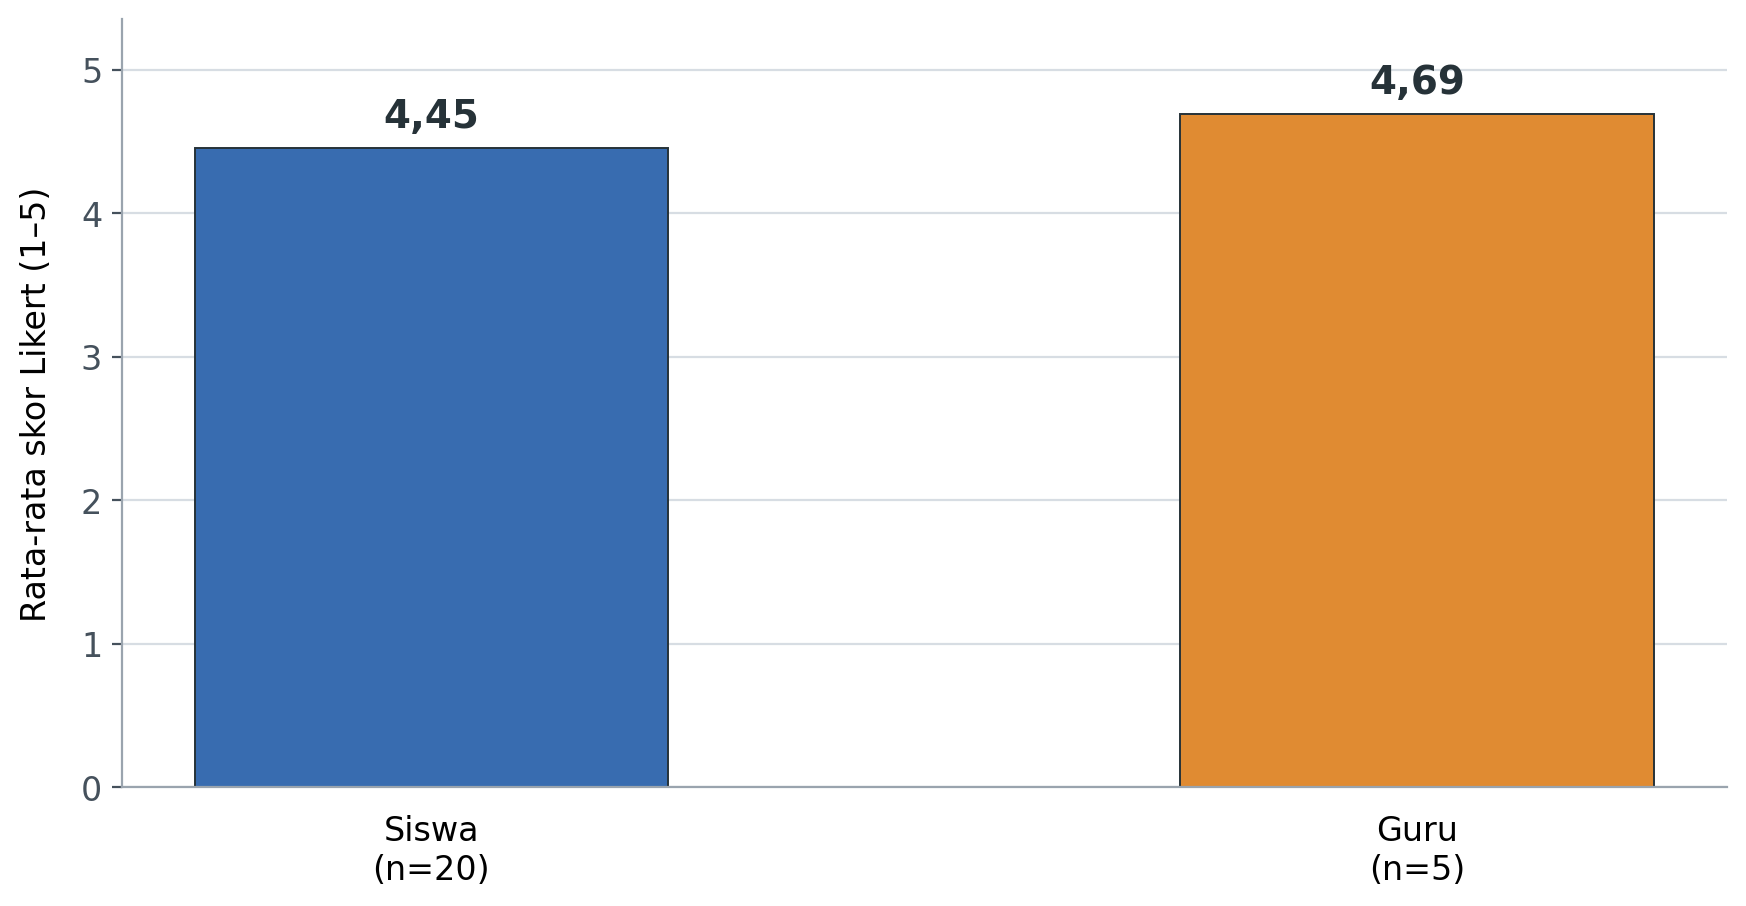
\includegraphics[width=0.85\linewidth]{gambar/grafik-4-4.png}
\caption{Perbandingan Rata-rata Keseluruhan Kuesioner Siswa dan Guru}\label{fig:4.4}
\end{figure}

Berdasarkan Gambar~\ref{fig:4.4}, rata-rata penilaian siswa adalah 4,45, sedangkan rata-rata penilaian guru adalah 4,69. Kedua nilai tersebut termasuk dalam kategori Sangat Baik. Rata-rata guru lebih tinggi 0,24 poin daripada rata-rata siswa. Perbandingan ini menggunakan skor keseluruhan tiap kelompok; jumlah dan butir pertanyaan pada kuesioner siswa dan guru berbeda, sehingga grafik tidak dimaksudkan sebagai perbandingan langsung untuk setiap aspek.

\section{REKAPITULASI HASIL PENGUJIAN}

Berdasarkan seluruh pengujian yang telah dilakukan, berikut adalah rekapitulasi hasil pengujian sistem InternSync secara keseluruhan yang disajikan pada Tabel~\ref{tab:4.12}.

{\singlespacing\small\renewcommand{\arraystretch}{1.25}
\begin{longtable}{|>{\raggedright\arraybackslash}p{\dimexpr(\linewidth-6\arrayrulewidth)*527/7938-2\tabcolsep\relax}|>{\raggedright\arraybackslash}p{\dimexpr(\linewidth-6\arrayrulewidth)*3288/7938-2\tabcolsep\relax}|>{\centering\arraybackslash}p{\dimexpr(\linewidth-6\arrayrulewidth)*975/7938-2\tabcolsep\relax}|>{\centering\arraybackslash}p{\dimexpr(\linewidth-6\arrayrulewidth)*1424/7938-2\tabcolsep\relax}|>{\centering\arraybackslash}p{\dimexpr(\linewidth-6\arrayrulewidth)*1724/7938-2\tabcolsep\relax}|}
\caption{Rekapitulasi Hasil Pengujian Sistem InternSync}\label{tab:4.12}\\
\hline
\rowcolor[HTML]{D9D9D9}\multicolumn{1}{|>{\centering\arraybackslash\bfseries}p{\dimexpr(\linewidth-6\arrayrulewidth)*527/7938-2\tabcolsep\relax}|}{No} & \multicolumn{1}{|>{\centering\arraybackslash\bfseries}p{\dimexpr(\linewidth-6\arrayrulewidth)*3288/7938-2\tabcolsep\relax}|}{Parameter Pengujian} & \multicolumn{1}{|>{\centering\arraybackslash\bfseries}p{\dimexpr(\linewidth-6\arrayrulewidth)*975/7938-2\tabcolsep\relax}|}{Total} & \multicolumn{1}{|>{\centering\arraybackslash\bfseries}p{\dimexpr(\linewidth-6\arrayrulewidth)*1424/7938-2\tabcolsep\relax}|}{Berhasil} & \multicolumn{1}{|>{\centering\arraybackslash\bfseries}p{\dimexpr(\linewidth-6\arrayrulewidth)*1724/7938-2\tabcolsep\relax}|}{Persentase} \\ \hline
\endfirsthead
\hline
\rowcolor[HTML]{D9D9D9}\multicolumn{1}{|>{\centering\arraybackslash\bfseries}p{\dimexpr(\linewidth-6\arrayrulewidth)*527/7938-2\tabcolsep\relax}|}{No} & \multicolumn{1}{|>{\centering\arraybackslash\bfseries}p{\dimexpr(\linewidth-6\arrayrulewidth)*3288/7938-2\tabcolsep\relax}|}{Parameter Pengujian} & \multicolumn{1}{|>{\centering\arraybackslash\bfseries}p{\dimexpr(\linewidth-6\arrayrulewidth)*975/7938-2\tabcolsep\relax}|}{Total} & \multicolumn{1}{|>{\centering\arraybackslash\bfseries}p{\dimexpr(\linewidth-6\arrayrulewidth)*1424/7938-2\tabcolsep\relax}|}{Berhasil} & \multicolumn{1}{|>{\centering\arraybackslash\bfseries}p{\dimexpr(\linewidth-6\arrayrulewidth)*1724/7938-2\tabcolsep\relax}|}{Persentase} \\ \hline
\endhead
1 & Fungsionalitas Peran Siswa & 10 & 10 & 100\% \\ \hline
2 & Fungsionalitas Peran Guru Pembimbing & 9 & 9 & 100\% \\ \hline
3 & Fungsionalitas Peran Koordinator PKL & 12 & 12 & 100\% \\ \hline
4 & Fungsionalitas Peran Hubin & 10 & 10 & 100\% \\ \hline
5 & Fungsionalitas Peran Admin Sistem & 6 & 6 & 100\% \\ \hline
6 & Keamanan Akses (RBAC) & 5 & 5 & 100\% \\ \hline
7 & Penanganan Kesalahan (Error Handling) & 6 & 6 & 100\% \\ \hline
8 & Responsivitas Antarmuka & 5 & 5 & 100\% \\ \hline
 & \textbf{Total Keseluruhan} & \textbf{63} & \textbf{63} & \textbf{100\%} \\ \hline
\end{longtable}}

Berdasarkan hasil rekapitulasi pada Tabel~\ref{tab:4.12}, dari total 63 skenario pengujian pada delapan parameter, seluruh skenario berhasil dijalankan dengan hasil yang sesuai. Parameter ke-9, yaitu kuesioner kepuasan pengguna, dibahas pada subbab 4.8 dan tidak dihitung sebagai skenario Black Box karena berupa penilaian subjektif. Tingkat keberhasilan 100\% pada seluruh parameter pengujian menunjukkan bahwa sistem InternSync siap diimplementasikan di lingkungan SMK PGRI Telagasari melalui domain \url{https://internsync.smkpgritelagasari.sch.id/.}

\chapter{PENUTUP}

\section{KESIMPULAN}

Berdasarkan hasil analisis, perancangan, dan pengujian yang telah dijabarkan pada bab-bab sebelumnya, dapat ditarik beberapa kesimpulan sebagai berikut:

\begin{enumerate}[label=\arabic*.]
\item Pelaksanaan Praktik Kerja Lapangan (PKL) di SMK PGRI Telagasari yang sebelumnya bergantung pada dokumen fisik menimbulkan risiko kehilangan data, lambatnya verifikasi administratif, dan sulitnya pemantauan secara real-time. Solusi yang ditawarkan untuk mengatasi masalah tersebut adalah pengembangan InternSync, yakni sebuah sistem informasi manajemen terintegrasi berbasis web.
\item Sistem ini mengintegrasikan alur administrasi PKL secara end-to-end melalui arsitektur client-server berbasis REST API terpusat. Sistem ini memadukan teknologi React pada \textit{frontend} web, Laravel pada \textit{backend} API, dan MySQL sebagai basis data, sedangkan aplikasi mobile berbasis Flutter masih berupa rencana pengembangan lanjutan. Sistem juga menjembatani komunikasi antara sekolah dan pihak industri melalui alur perizinan berbasis tautan token dan penilaian kinerja berbasis rubrik baku.
\item Hasil pengujian menggunakan metode Black Box Testing menunjukkan tingkat keberhasilan 100\% dari 63 skenario pengujian fungsional dan keamanan.
\item Pengujian melalui kuesioner membuktikan bahwa sistem sangat efektif dalam menyelesaikan masalah administrasi, yang ditunjukkan dengan rata-rata skor kepuasan sebesar 4,45 (Sangat Baik) dari sisi siswa dan 4,69 (Sangat Baik) dari sisi guru pembimbing maupun koordinator. InternSync terbukti mempercepat birokrasi, mengeliminasi risiko data fisik terfragmentasi, dan mendukung visi Smart School di SMK PGRI Telagasari.
\end{enumerate}

\section{SARAN}

Meskipun aplikasi web InternSync telah berhasil diimplementasikan, terdapat beberapa keterbatasan yang dapat dijadikan landasan untuk pengembangan dan peningkatan sistem di masa mendatang:

\begin{enumerate}[label=\arabic*.]
\item Merealisasikan aplikasi mobile berbasis Flutter bagi Siswa dan Guru Pembimbing sesuai rancangan pada subbab 3.3, yang terhubung ke REST API yang sama dengan aplikasi web, mencakup login, dasbor, pencatatan logbook dengan foto dari kamera ponsel, pengajuan izin/sakit, dan pemantauan siswa bimbingan.
\item Setelah aplikasi mobile terealisasi, perlu adanya integrasi sistem push notification serta fitur notifikasi pengingat (reminder) otomatis untuk pengisian logbook siswa agar respon pengawasan dapat berjalan lebih cepat.
\item Integrasi WhatsApp Business API Gateway otomatis untuk pengiriman tautan tokenized persetujuan izin presensi dan formulir rubrik evaluasi langsung ke kontak nomor telepon pembimbing industri secara instan, guna meningkatkan kecepatan respon industri di lapangan.
\item Modul evaluasi dan pengawasan perlu diperluas dengan menambahkan fitur unggah dokumentasi (seperti foto kunjungan industri) bagi guru pembimbing saat melakukan supervisi ke lokasi industri.
\item Fitur rekapitulasi dan ekspor laporan akhir (report) disarankan agar dikembangkan dengan kapabilitas kustomisasi format output, sehingga dapat lebih fleksibel beradaptasi dengan perubahan standar administrasi sekolah.
\item Peningkatan pada aspek desain antarmuka (UI/UX) pada sisi pengguna siswa agar tampilannya lebih modern dan memfasilitasi penambahan modul galeri foto kegiatan harian.
\end{enumerate}


% ---------------------------- DAFTAR PUSTAKA ------------------------------------------
\clearpage
\phantomsection\addcontentsline{toc}{chapter}{DAFTAR PUSTAKA}
\begingroup
\singlespacing
\setlength{\itemsep}{6pt}
\setlength{\parindent}{0pt}\raggedright
\renewcommand{\bibname}{DAFTAR PUSTAKA}
\makeatletter
\renewenvironment{thebibliography}[1]
     {\chapter*{\bibname}%
      \list{\@biblabel{\@arabic\c@enumiv}}%
           {\settowidth\labelwidth{\@biblabel{99}}%
            \leftmargin\labelwidth
            \advance\leftmargin\labelsep
            \setlength{\itemsep}{6pt}\setlength{\parsep}{0pt}%
            \usecounter{enumiv}%
            \let\p@enumiv\@empty
            \renewcommand\theenumiv{\@arabic\c@enumiv}}%
      \sloppy
      \clubpenalty4000 \@clubpenalty \clubpenalty
      \widowpenalty4000%
      \sfcode`\.\@m}
     {\def\@noitemerr
       {\@latex@error{Empty `thebibliography' environment}\@ehc}%
      \endlist}
\makeatother
\begin{thebibliography}{99}
\bibitem{ref1} I. A. Alfarisi, A. T. Priandika, and A. S. Puspaningrum, “Penerapan Framework Laravel Pada Sistem Pelayanan Kesehatan (Studi Kasus: Klinik Berkah Medical Center),” J. Ilm. Comput. Sci., vol. 2, no. 1, pp. 1–9, 2023, doi: 10.58602/jics.v2i1.11.
\bibitem{ref2} M. S. Deni Murdiani, “PERBANDINGAN METODOLOGI WATERFALL DAN RAD (RAPID APPLICATION DEVELOPMENT) DALAM PENGEMBANGAN SISTEM INFORMASI,” vol. 4, no. 4, pp. 302–306, 2022.
\bibitem{ref3} H. N. Ningsih, Widya, “PERBANDINGAN MODEL WATERFALL DAN METODE PROTOTYPE UNTUK PENGEMBANGAN APLIKASI PADA SISTEM INFORMASI,” vol. 5, no. 1, pp. 83–95, 2023.
\bibitem{ref4} M. T. P. Perdana, G. Farell, T. Sriwahyuni, and L. Mursyida, “Design and Implementation of a Web-Based Internship Management Information System for Vocational Education,” J. Vokasi Inform., vol. 5, no. 2, pp. 286– 304, 2025.
\bibitem{ref5} M. Nugraha, R. Agus, H. Fathi, and R. Baginda, “Development a Web-Based Student Internship Application Using Laravel Framework,” J. Inf. Technol. Its Util., vol. 6, no. 1, pp. 31–38, 2023, doi: 10.56873/jitu.6.1.5139.
\bibitem{ref6} H. D. Yulianto and R. B. Firdaus, “Perancangan Sistem Informasi Monitoring Magang,” IJIS - Indonesian J. Inf. Syst., vol. 6, no. 2, pp. 130--136, 2021, doi: 10.36549/ijis.v6i2.144.
\bibitem{ref7} F. Moeinzadeh, S. H. R. Ayati, B. Iraj, M. Mortazavi, and V. Vafamehr, “Designing, implementation, and evaluation of internship comprehensive system for assessment and monitoring,” J. Educ. Health Promot., vol. 10, art. no. 93, 2021, doi: 10.4103/jehp.jehp\_626\_20.
\bibitem{ref8} M. Anas, U. M. Putri, and M. Yusuf, “Sistem Informasi Manajemen Praktek Kerja Lapangan ( PKL ) Berbasis Website pada PT . Perkebunan Nusantara IV Regional IV Kota Jambi Menggunakan Extreme Programming,” vol. 4, no. 2, pp. 1059–1069, 2025.
\bibitem{ref9} M. Arkan, R. Razan, I. Arwani, and H. Farisi, “Pengembangan Aplikasi Monitoring dan Evaluasi Kinerja Siswa Magang dari Indonesia Learning Center berbasis Android,” J. Pengemb. Teknol. Inf. dan Ilmu Komput., vol. 7, no. 5, pp. 2091–2100, 2023, [Online]. Available: \url{http://j-ptiik.ub.ac.id}
\bibitem{ref10} A. A. Samudra et al., “PERANCANGAN SISTEM INFORMASI MANAJEMEN PRAKTIK KERJA LAPANGAN ( PKL ) BERBASIS WEB DI SMK NEGERI 1 BUNGO,” vol. 7, no. 5, pp. 3497–3503, 2023.
\bibitem{ref11} B. Bestin, M. G. Addiansyah, R. Sofian, F. Reza, and M. N. Wafa, “Sistem Informasi Monitoring Peserta Magang Berbasis Web Pada Divisi Sales \& Business Development Di Mayar Kota Bandung,” vol. 14, no. 2, pp. 163–170, 2023.
\bibitem{ref12} F. K. Dewi, E. Purwanto, and H. Permatasari, “Sistem Informasi Monitoring Praktik Kerja Lapangan Siswa Berbasis Web Di SMK Ma ’ arif Nu 2 Boyolali,” pp. 637–647, 2024.
\bibitem{ref13} M. Ilmi, D. R. Habibie, and Y. Arifin, “Analisis dan Perancangan Sistem Informasi Monitoring Siswa PKL pada SMK Permata Harapan,” JOINS (Journal Inf. Syst., vol. 8, no. 2, pp. 177–187, 2023, doi: 10.33633/joins.v8i2.9233.
\bibitem{ref14} N. F. Syahidannur Mukminah Pulungan, Reza Febrianti, Titin Lestari, Natra Gurning, “Analisis Teknik Entity-Relationship Diagram Dalam Perancangan Database,” vol. 2, no. 1, pp. 98–102, 2023.
\bibitem{ref15} I. R. Mukhlis and R. Santoso, “Perancangan Basis Data Perpustakaan Universitas Menggunakan MySQL dengan Physical Data Model dan Entity Relationship Diagram,” vol. 4, no. 2, pp. 2–8, 2023, doi: 10.37802/joti.v4i2.330.
\bibitem{ref16} F. Renardi, N. Faizah, and L. Koryanto, “Reimbursement Application Using Rest API Methods and Android-Based Flutter Framework (Case Study: PT. Protonema),” J. Mob. Technol., vol. 1, no. 1, pp. 44–52, 2023, doi: 10.59431/jms.v1i1.133.
\bibitem{ref17} Y. L. Pattinama and I. Susanti, “Implementasi Rest API Web Service Dengan Otentifikasi JSON Web Token Untuk Aplikasi Properti,” vol. 4221, no. April, pp. 81–89, 2023.
\bibitem{ref18} A. S. F. Ferry Kurniawan, Erlin Ayu Khrisnawati, Rizka Hadiwiyanti, “PENGUJIAN SISTEM INFORMASI MANAJEMEN SISWA BERBASIS WEBSITE MENGGUNAKAN METODE BLACK BOX DAN WHITE BOX Ferry,” no. September, pp. 10–11, 2022.
\bibitem{ref19} A. S. Wulandari, A. Saepudin, M. P. Kinanti, Z. Sudesi, A. Saifudin, and Y. Yulianti, “Pengujian Aplikasi Sistem Informasi Akademik Berbasis Web Menggunakan Metode Black Box Testing Equivalence Partitioning,” J. Teknol. Sist. Inf. dan Apl., vol. 5, no. 2, p. 102, 2022, doi: 10.32493/jtsi.v5i2.17561.
\bibitem{ref20} I. Permatasari, F. Adhania, S. A. Putri, and S. R. C. Nursari, “Pengujian Black Box Menggunakan Metode Analisis Nilai Batas pada Aplikasi DANA,” KONSTELASI Konvergensi Teknol. dan Sist. Inf., vol. 3, no. 2, pp. 373–387, 2023, doi: 10.24002/konstelasi.v3i2.8289.
\end{thebibliography}

\endgroup

% ---------------------------- LAMPIRAN -----------------------------------------------
\clearpage
\phantomsection\addcontentsline{toc}{chapter}{LAMPIRAN}
\chapter*{LAMPIRAN}
Lampiran berisi dokumen pendukung dan tangkapan layar yang menunjang pembahasan proyek akhir.

\setcounter{figure}{0}
\renewcommand{\thefigure}{L.\arabic{figure}}
\captionsetup{hypcap=false}

\section*{Rekapitulasi Kuesioner InternSync}
\addcontentsline{toc}{section}{Rekapitulasi Kuesioner InternSync}

{\small
\noindent\textbf{Link Responden Siswa:}\par
\noindent\href{https://docs.google.com/forms/d/e/1FAIpQLSf-MIfhVixnjja9oZIZ9ugWZsfemnbiRVDqD0d2gpPSG5jwow/viewform}{\texttt{https://docs.google.com/forms/d/e/1FAIpQLSf-MIfhVixnjja9oZIZ9ugW}\\\texttt{ZsfemnbiRVDqD0d2gpPSG5jwow/viewform}}\par
\noindent\textbf{Link Responden Guru:}\par
\noindent\href{https://docs.google.com/forms/d/e/1FAIpQLSduP57CQ_8BKu3W4xbrgNGjhA2UW4OOY5X_p_qyXWZXBjylFQ/viewform}{\texttt{https://docs.google.com/forms/d/e/1FAIpQLSduP57CQ\_8BKu3W4xbrgNGjh}\\\texttt{A2UW4OOY5X\_p\_qyXWZXBjylFQ/viewform}}\par
}
\newgeometry{left=1.5cm,right=1.5cm,top=1.5cm,bottom=3cm}

\begin{center}
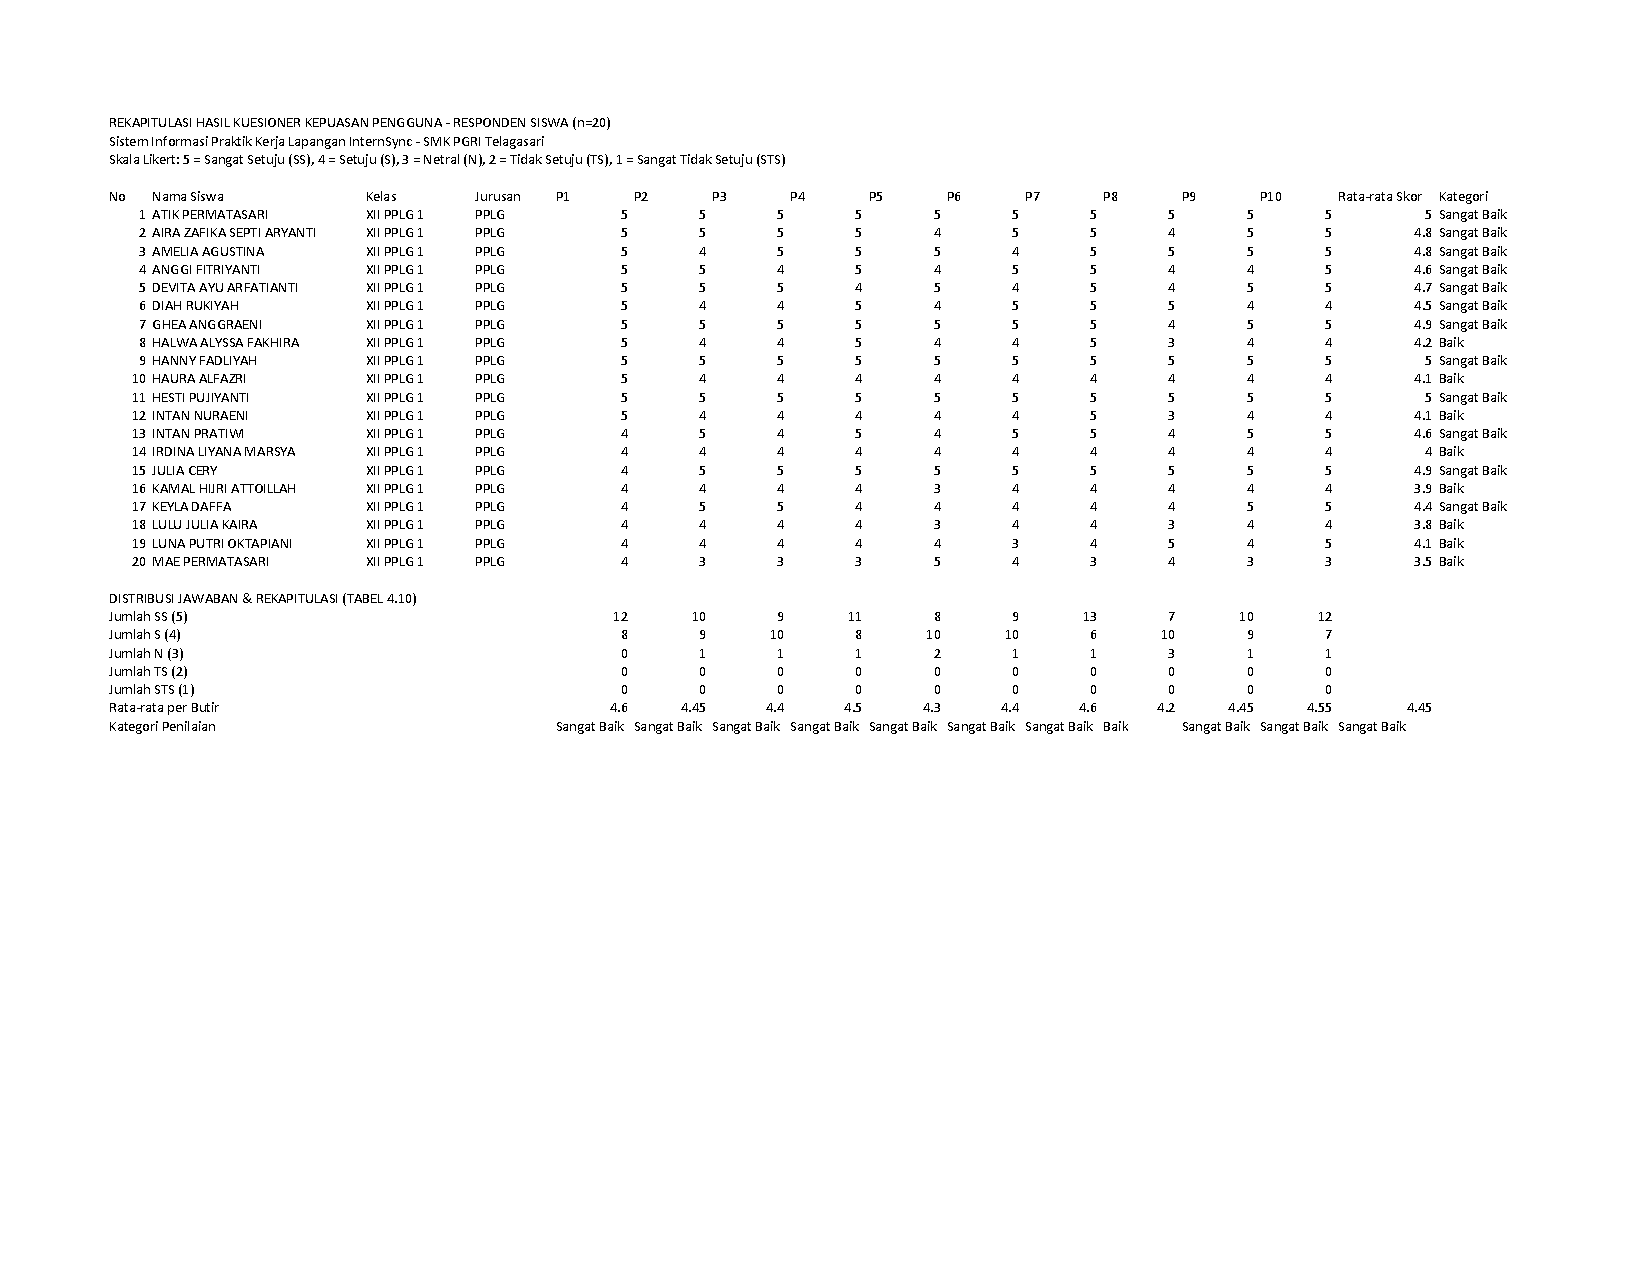
\includegraphics[page=1,angle=90,width=0.96\textheight,height=0.96\textwidth,keepaspectratio,frame]{lampiran/Rekapitulasi_Kuesioner_InternSync.pdf}
\captionof{figure}{Rekapitulasi Kuesioner InternSync (Halaman 1)}\label{fig:lampiran-kuesioner-1}
\end{center}
\clearpage

\begin{center}
\includegraphics[page=2,angle=90,width=0.96\textheight,height=0.96\textwidth,keepaspectratio,frame]{lampiran/Rekapitulasi_Kuesioner_InternSync.pdf}
\captionof{figure}{Rekapitulasi Kuesioner InternSync (Halaman 2)}\label{fig:lampiran-kuesioner-2}
\end{center}
\clearpage

\begin{center}
\adjustbox{angle=90,width=0.96\textheight,height=0.96\textwidth,keepaspectratio,frame}{%
\begin{tikzpicture}[x=1bp,y=1bp]
\path[use as bounding box] (0,0) rectangle (792,612);
\node[anchor=south west,inner sep=0pt] at (0,0)
  {\includegraphics[page=3,width=792bp,height=612bp,keepaspectratio]{lampiran/Rekapitulasi_Kuesioner_InternSync.pdf}};
\fill[white] (49,530) rectangle (350,548);
\node[anchor=west,inner sep=0pt,font=\sffamily\fontsize{8.18bp}{9bp}\selectfont] at (52.44,539.04)
  {Berdasarkan Laporan Subbab 4.9 (Tabel 4.12) \& Subbab 4.8 (Kuesioner Kepuasan)};
\end{tikzpicture}}
\captionof{figure}{Rekapitulasi Kuesioner InternSync (Halaman 3)}\label{fig:lampiran-kuesioner-3}
\end{center}
\clearpage

\begin{center}
\includegraphics[page=4,angle=90,width=0.96\textheight,height=0.96\textwidth,keepaspectratio,frame]{lampiran/Rekapitulasi_Kuesioner_InternSync.pdf}
\captionof{figure}{Rekapitulasi Kuesioner InternSync (Halaman 4)}\label{fig:lampiran-kuesioner-4}
\end{center}
\clearpage

\restoregeometry
\clearpage

\section*{Dokumen PDF Pendukung}
\addcontentsline{toc}{section}{Dokumen PDF Pendukung}

\begin{center}
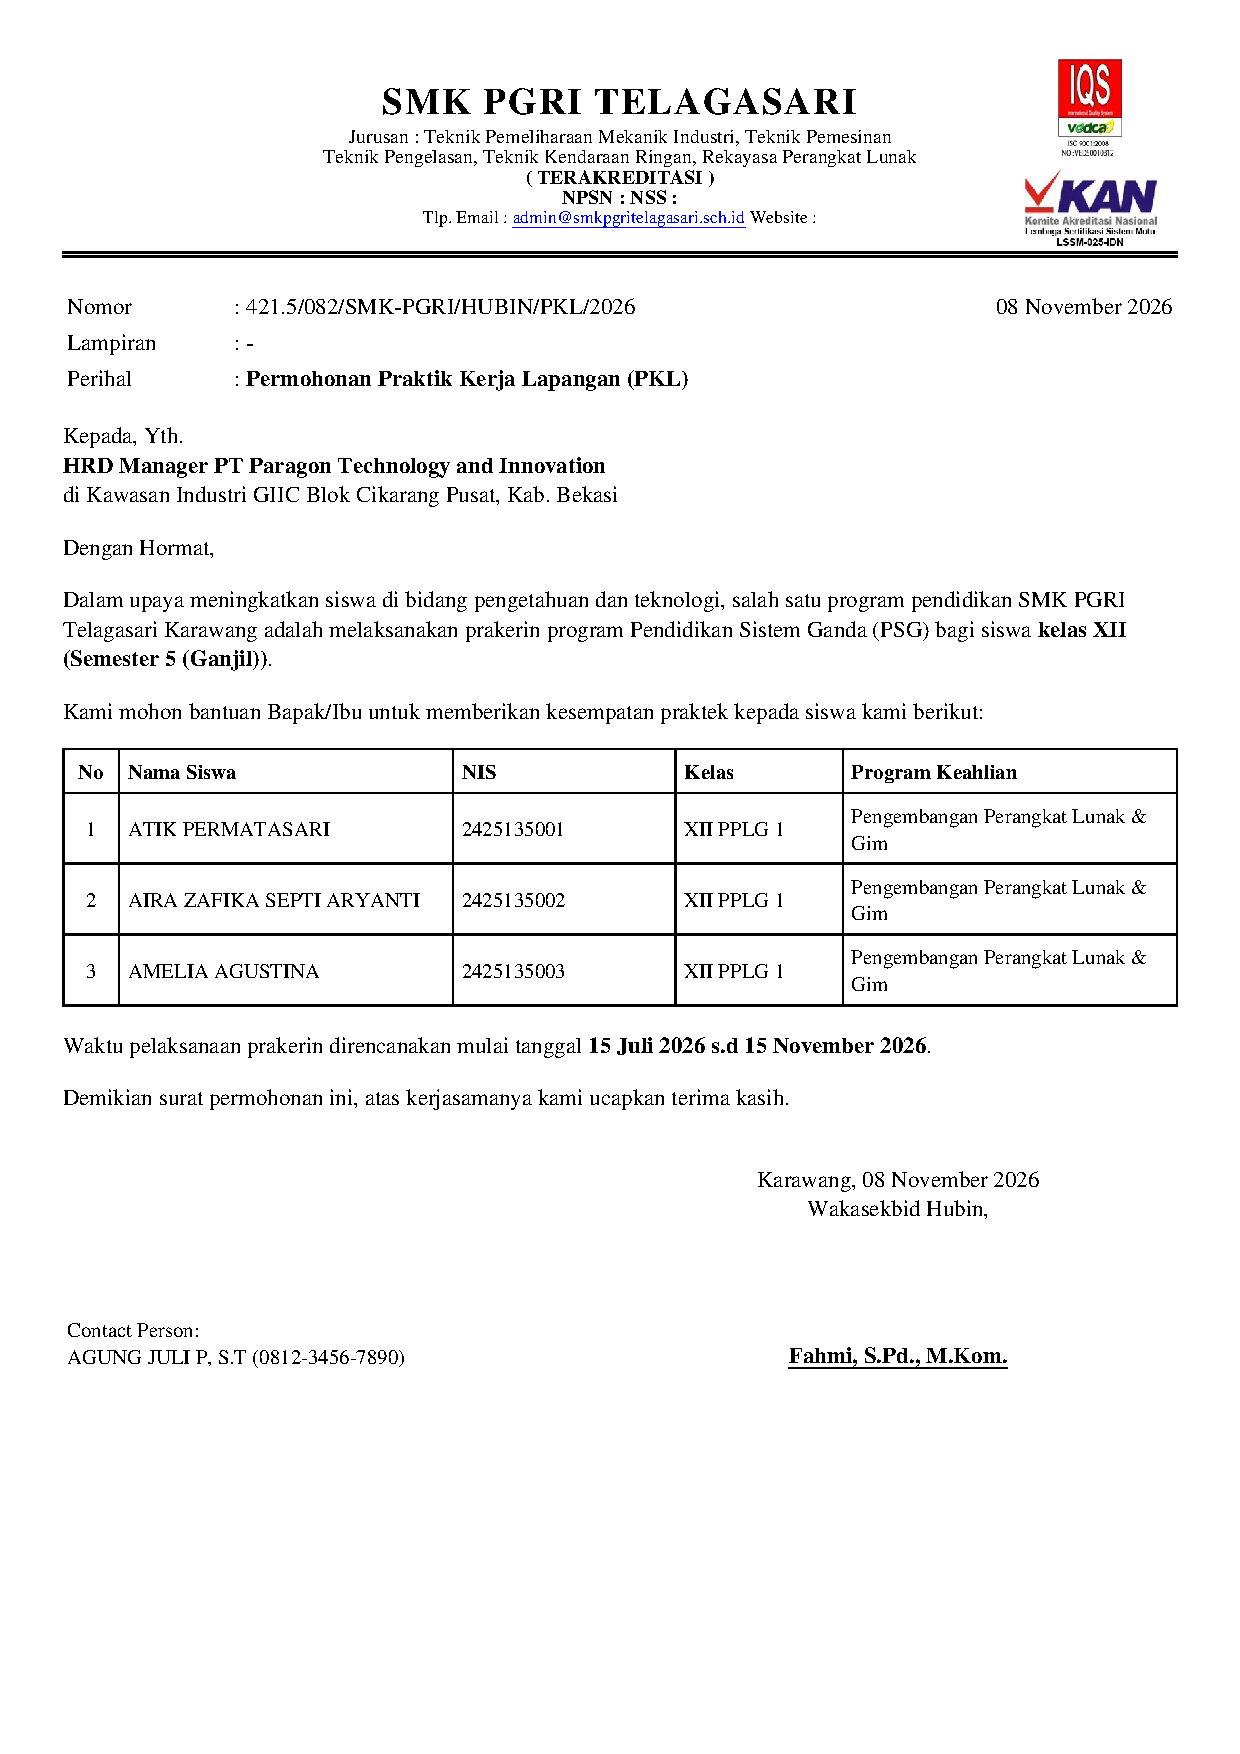
\includegraphics[page=1,width=0.90\textwidth,height=0.72\textheight,keepaspectratio,frame]{lampiran/1_Surat_Pengajuan_PKL.pdf}
\captionof{figure}{Surat Pengajuan PKL}\label{fig:lampiran-01}
\end{center}
\clearpage

\begin{center}
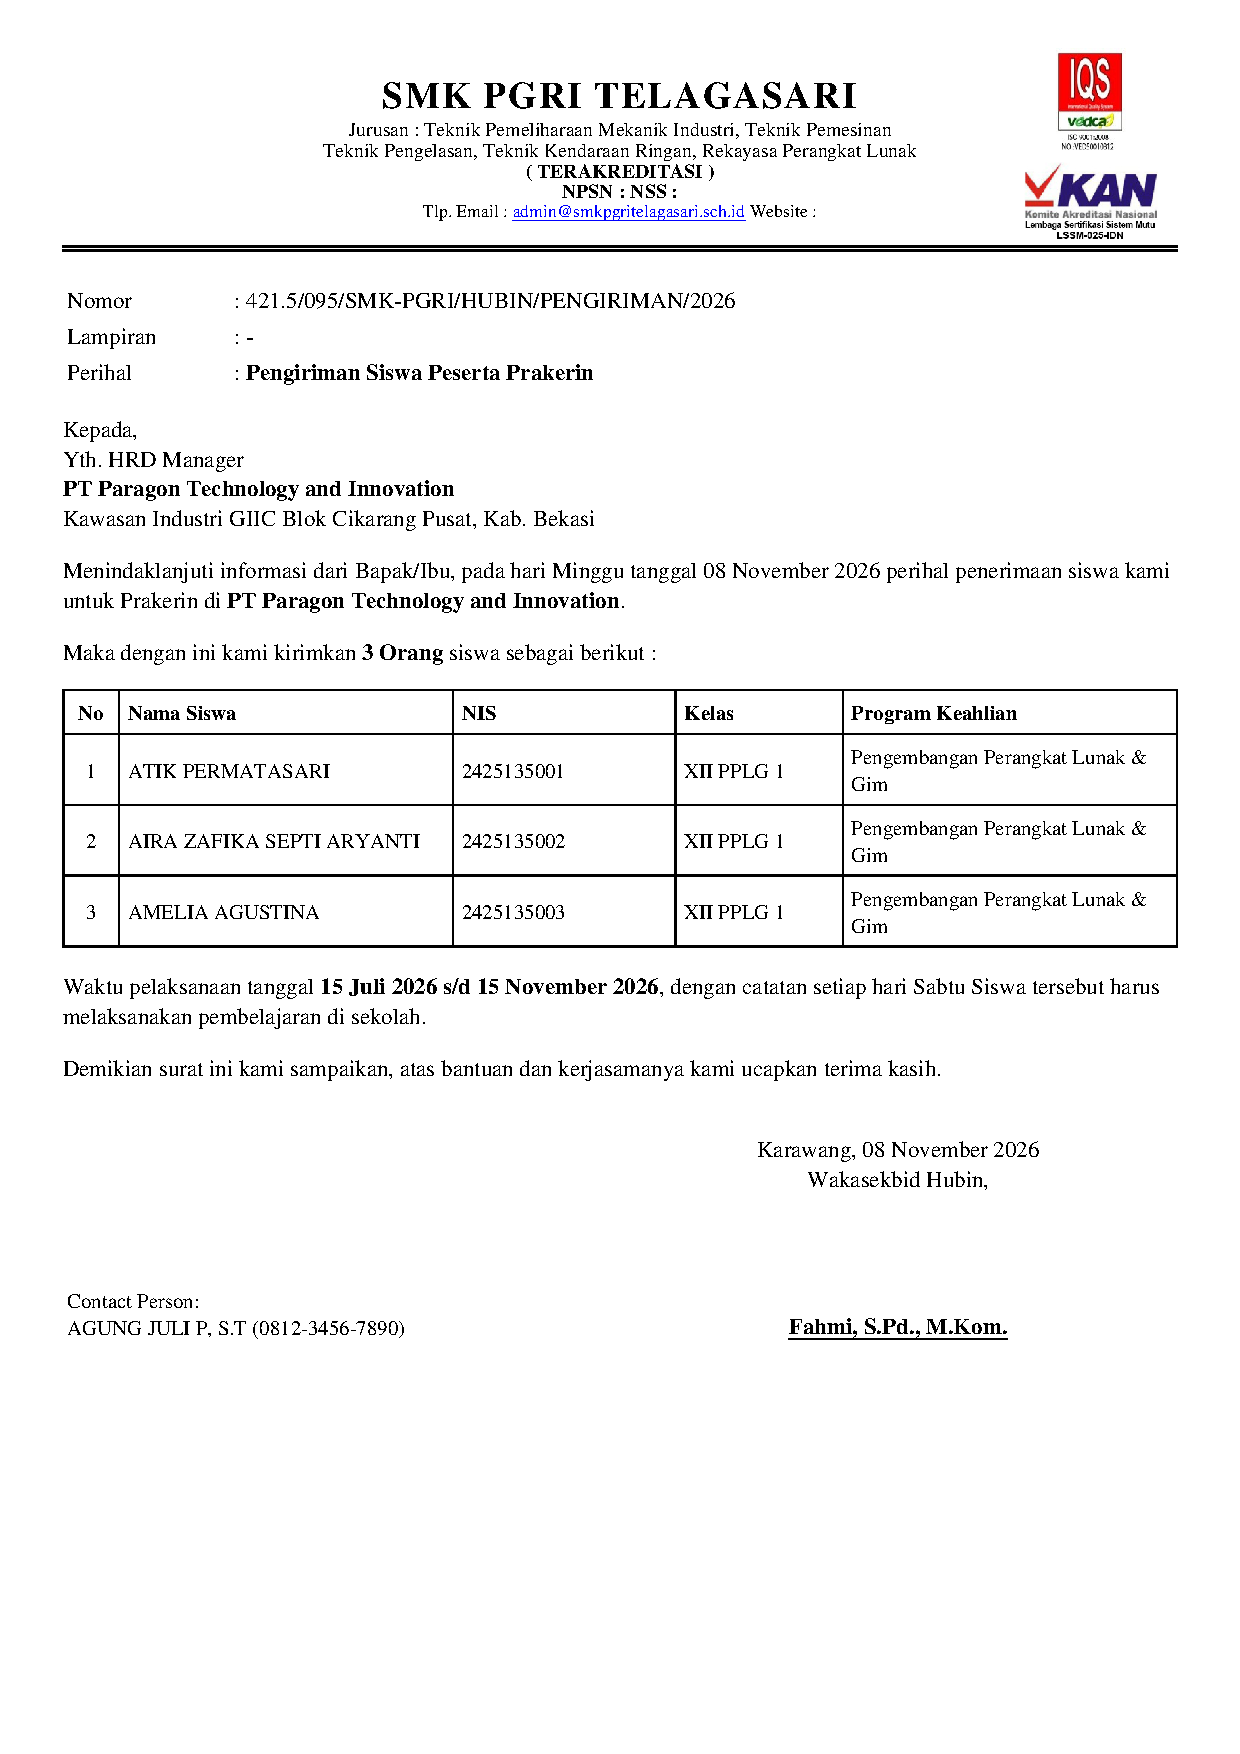
\includegraphics[page=1,width=0.90\textwidth,height=0.72\textheight,keepaspectratio,frame]{lampiran/2_Surat_Pengiriman_Siswa.pdf}
\captionof{figure}{Surat Pengiriman Siswa PKL}\label{fig:lampiran-02}
\end{center}
\clearpage

\begin{center}
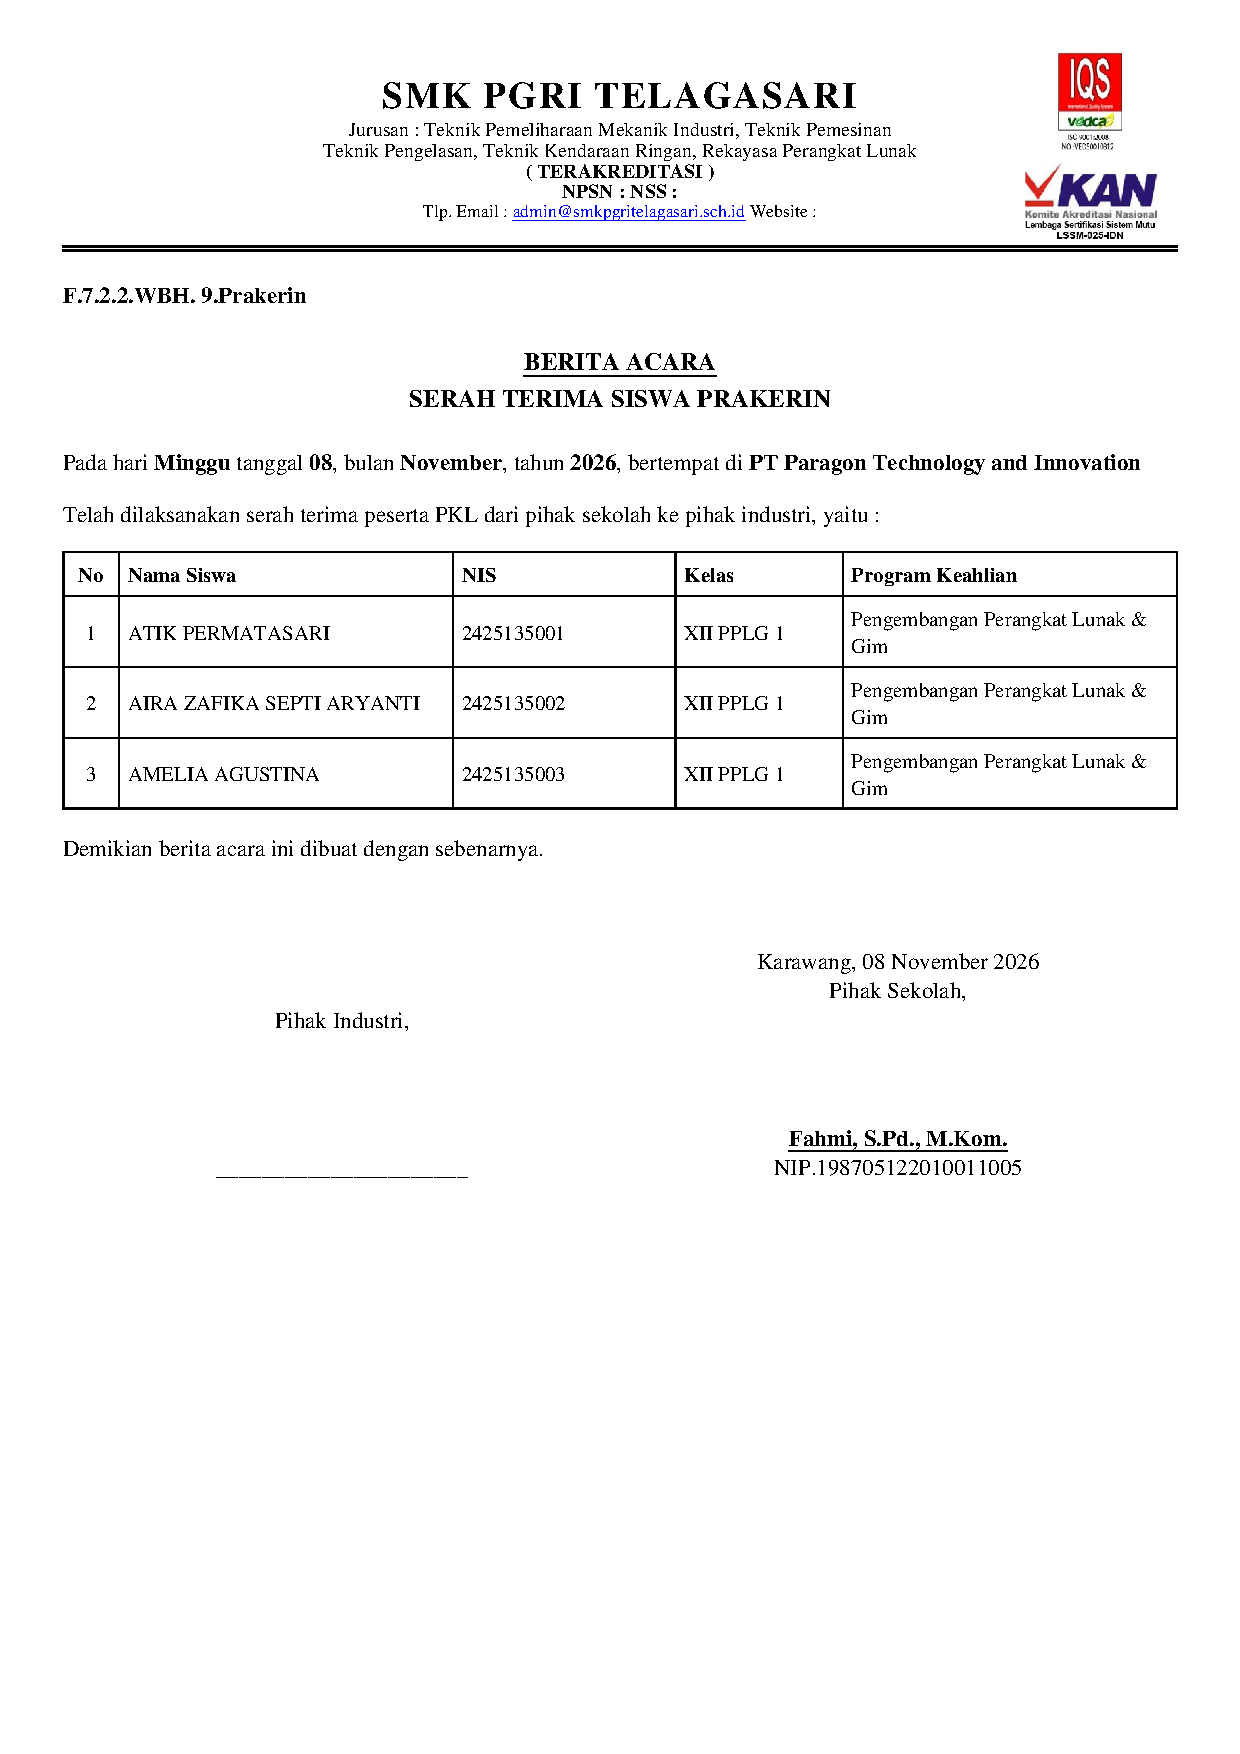
\includegraphics[page=1,width=0.90\textwidth,height=0.72\textheight,keepaspectratio,frame]{lampiran/3_Berita_Acara_Serah_Terima.pdf}
\captionof{figure}{Berita Acara Serah Terima Siswa PKL}\label{fig:lampiran-03}
\end{center}
\clearpage

\begin{center}
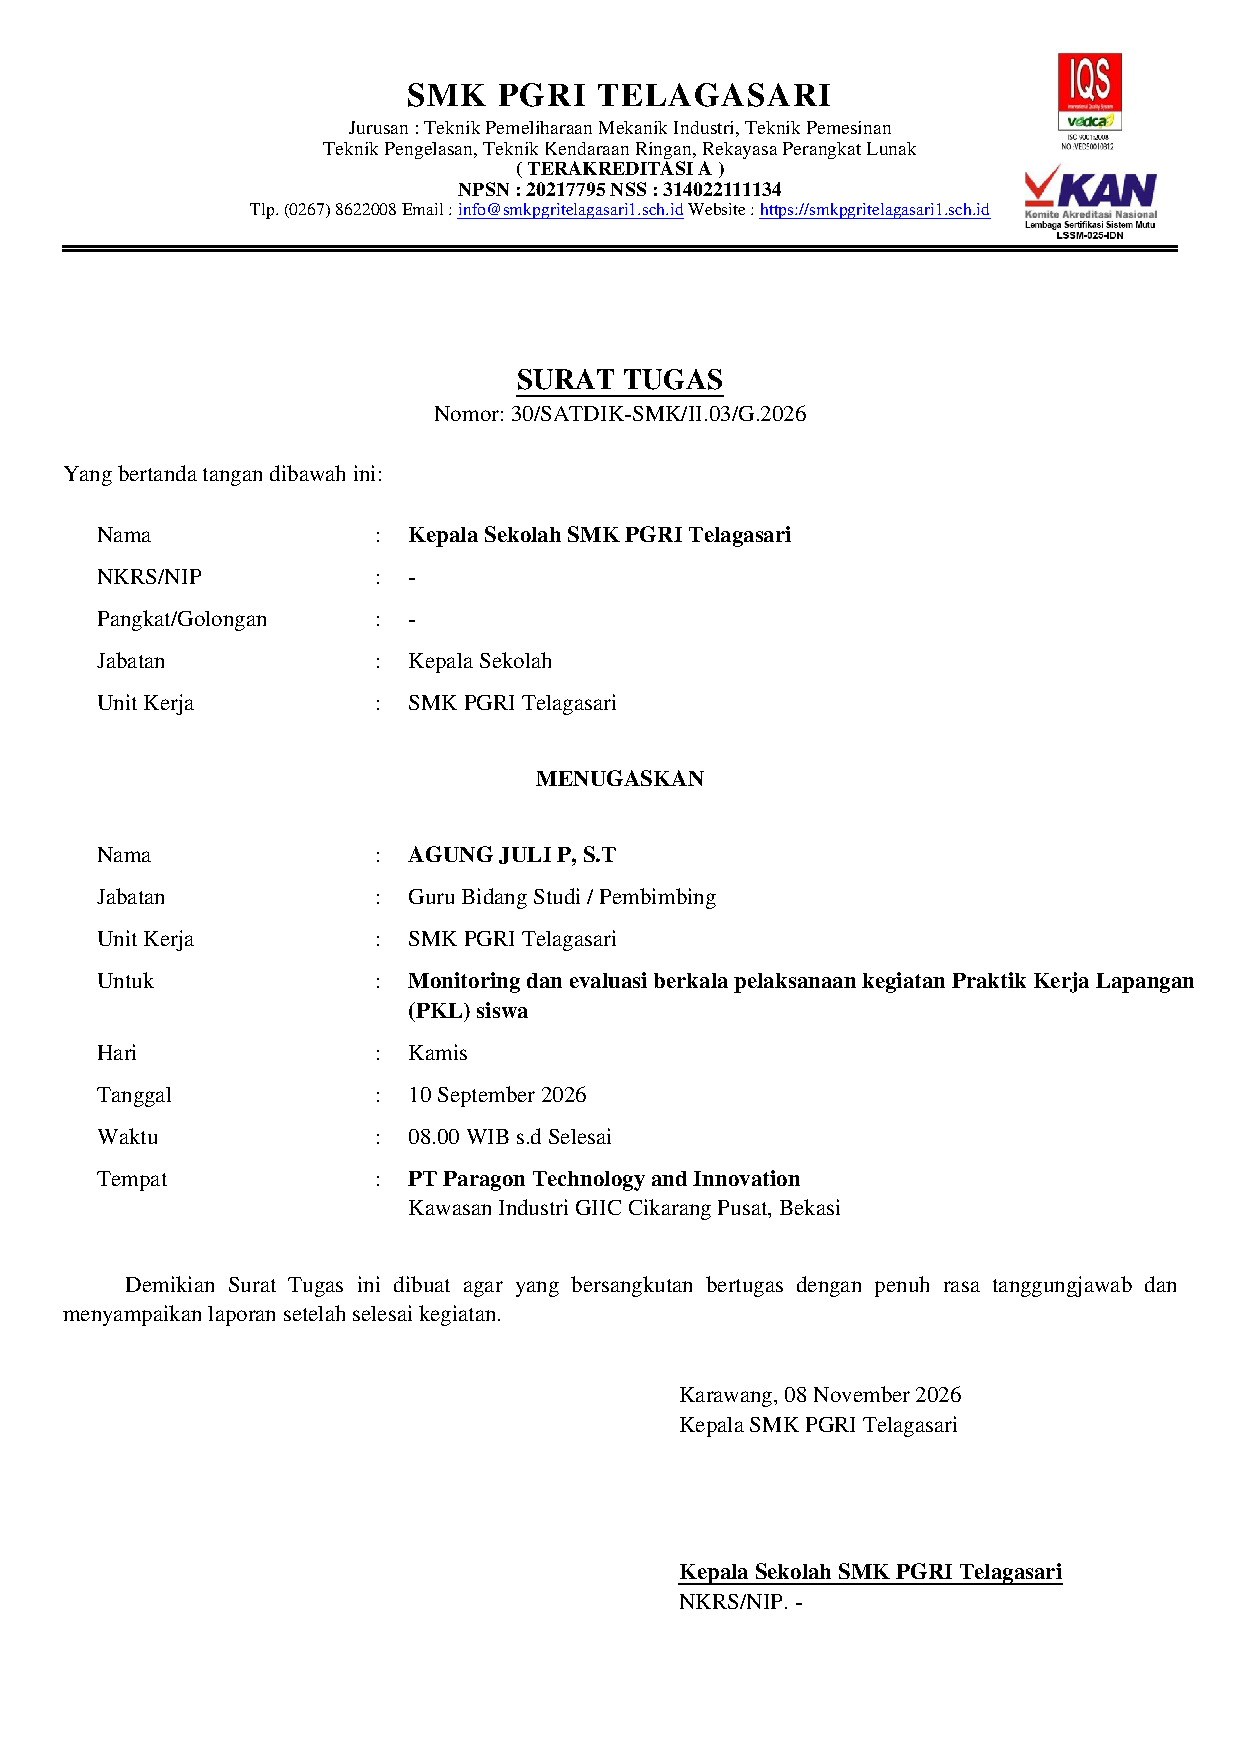
\includegraphics[page=1,width=0.90\textwidth,height=0.72\textheight,keepaspectratio,frame]{lampiran/4_SPPD_Kunjungan_Industri.pdf}
\captionof{figure}{Surat Perintah Perjalanan Dinas Kunjungan Industri}\label{fig:lampiran-04}
\end{center}
\clearpage

\begin{center}
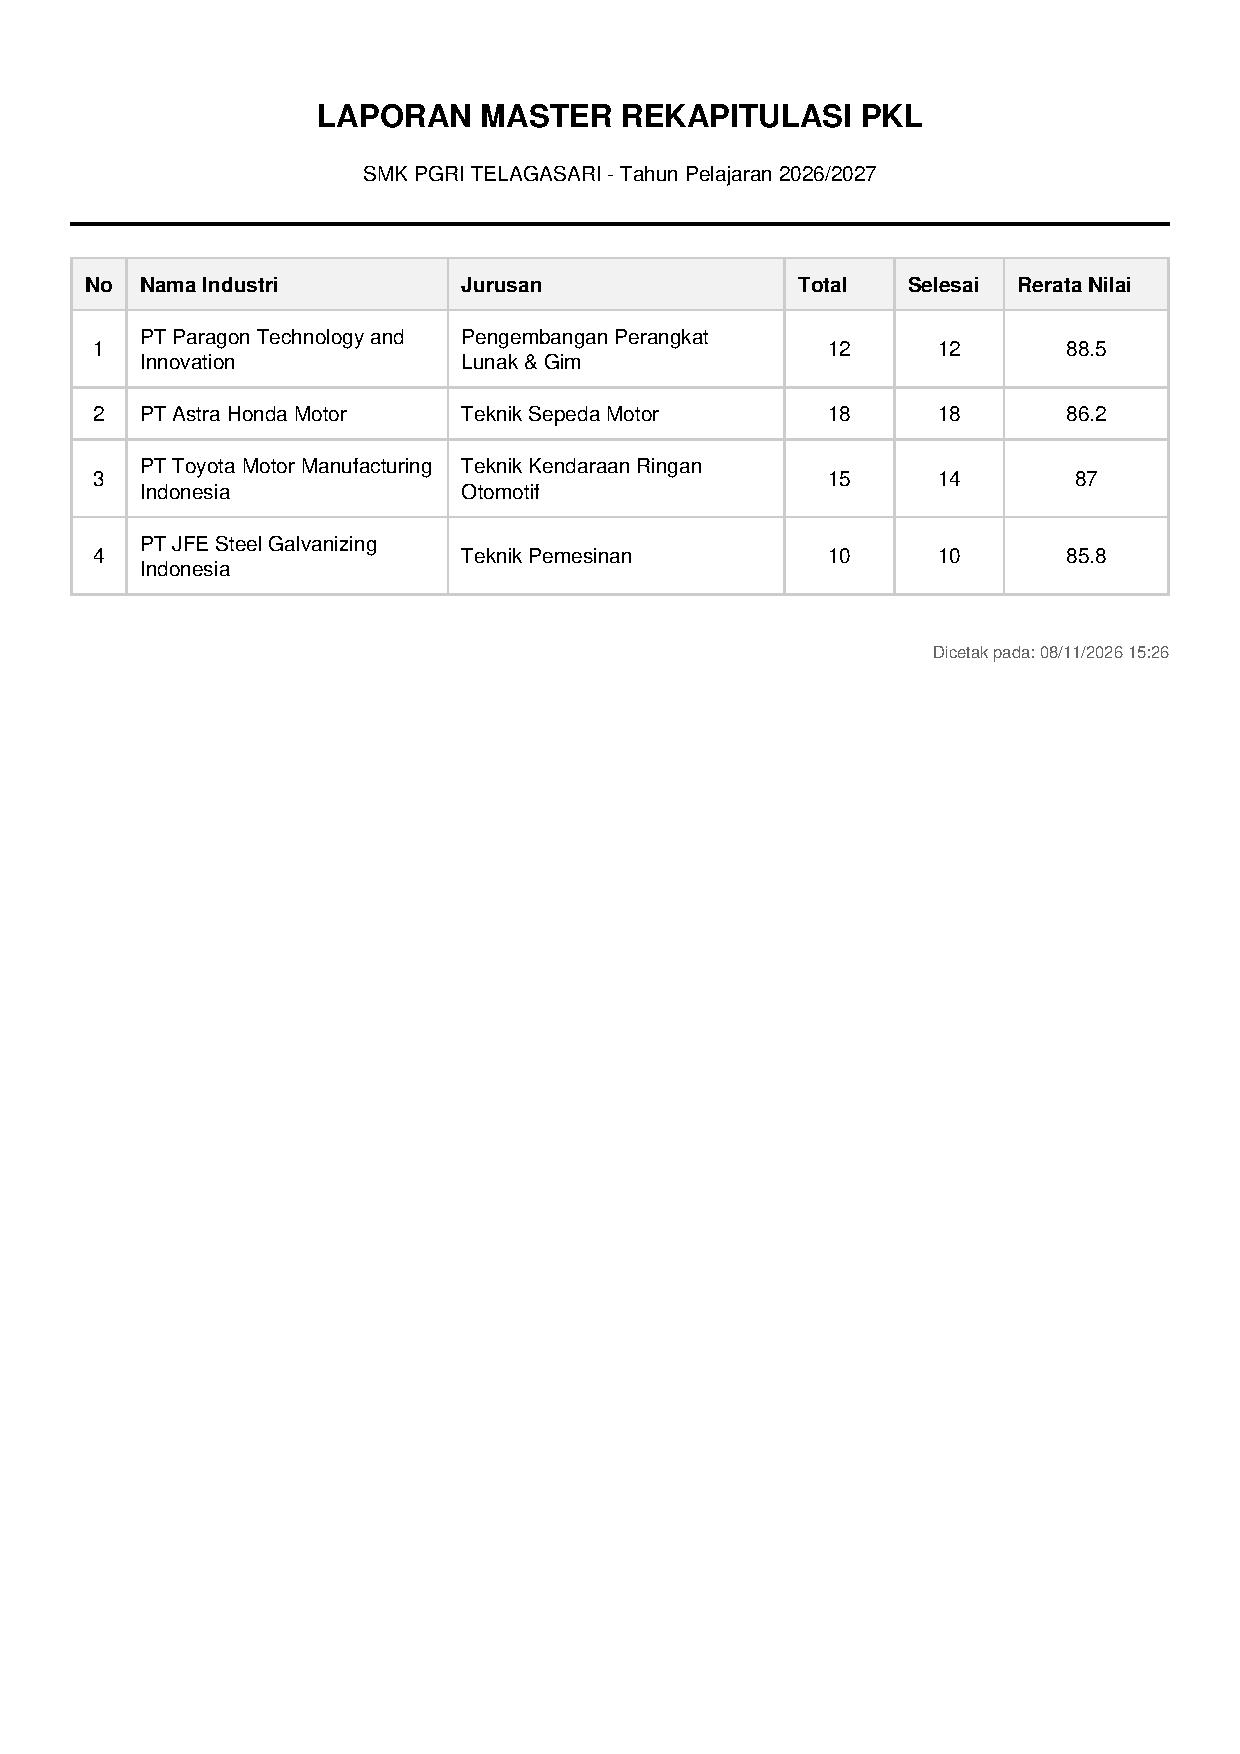
\includegraphics[page=1,width=0.90\textwidth,height=0.72\textheight,keepaspectratio,frame]{lampiran/5_Laporan_Master_Rekap_PKL.pdf}
\captionof{figure}{Laporan Master Rekapitulasi PKL}\label{fig:lampiran-05}
\end{center}
\clearpage

\begin{center}
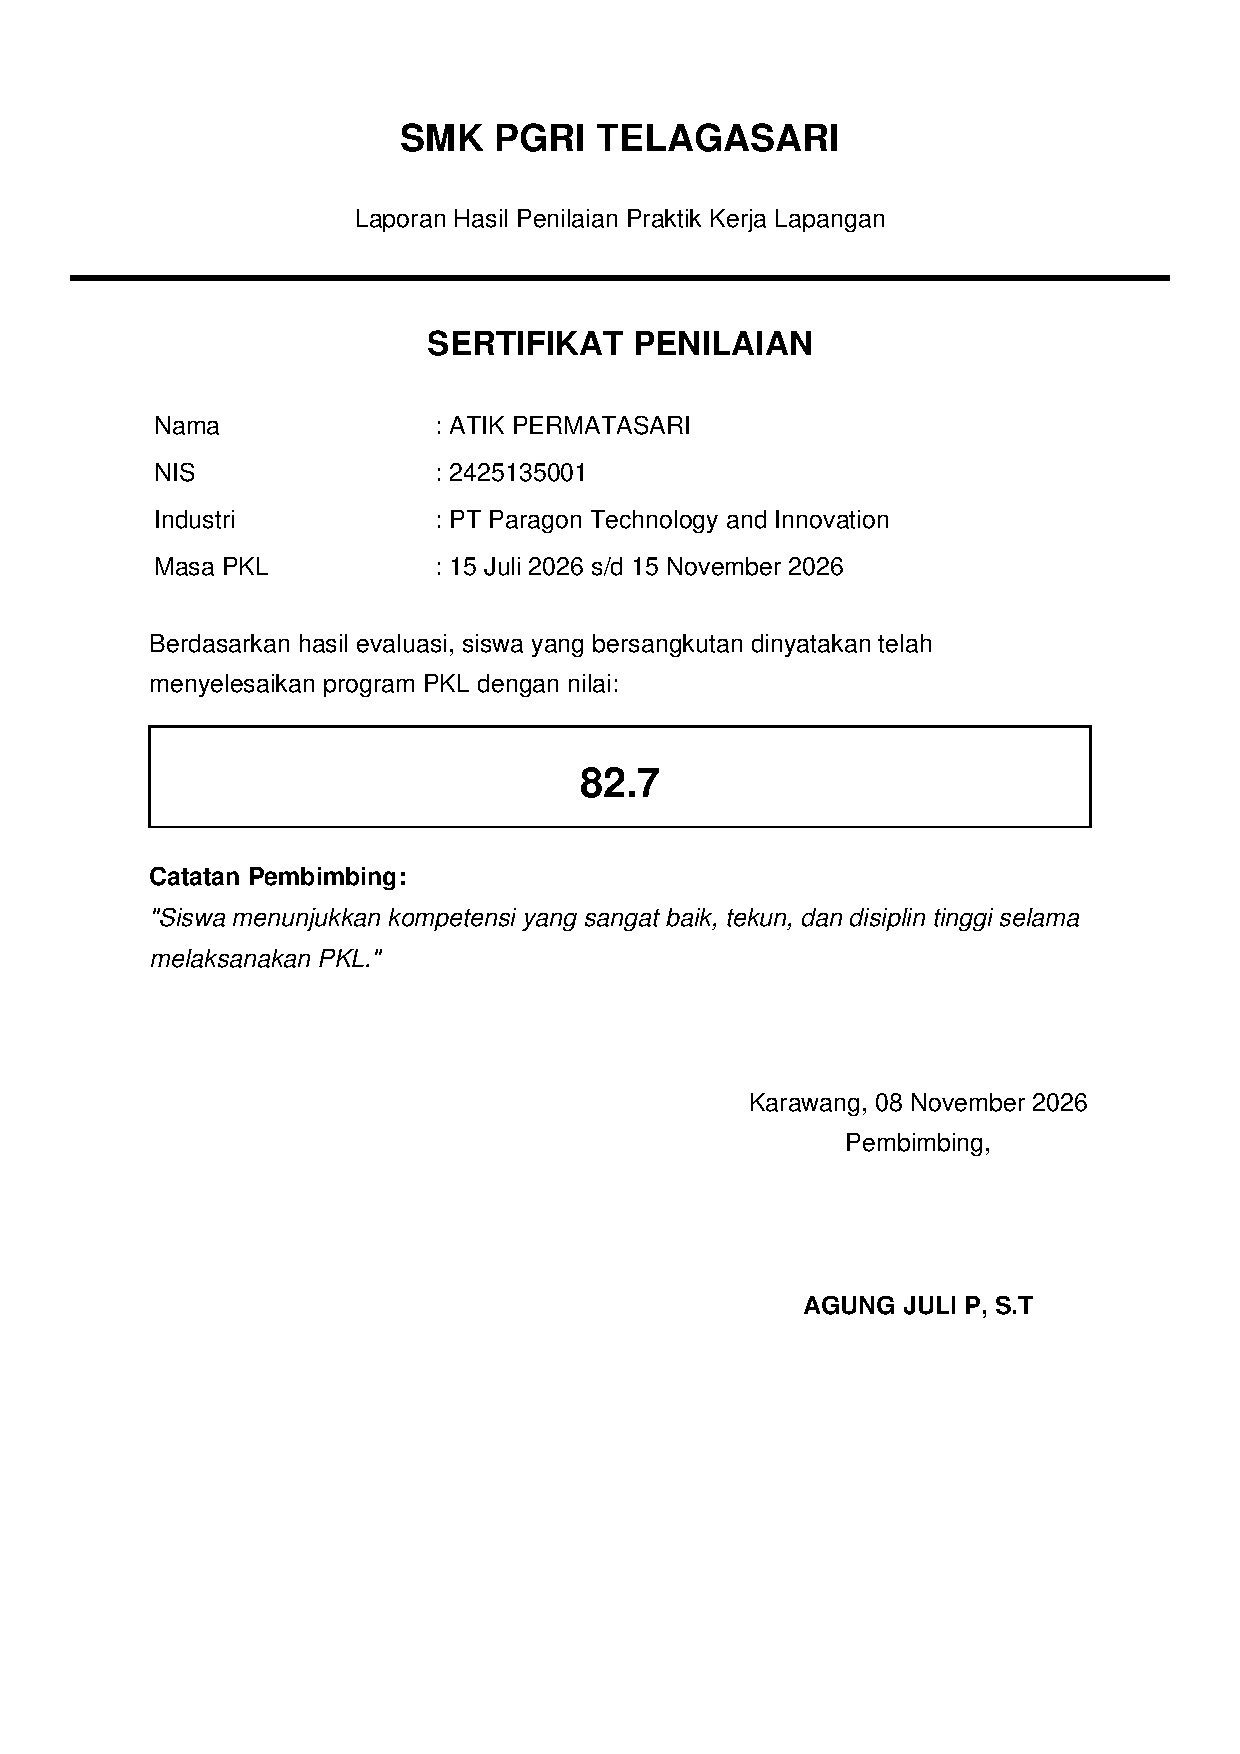
\includegraphics[page=1,width=0.90\textwidth,height=0.72\textheight,keepaspectratio,frame]{lampiran/8_Rapor_Nilai_PKL_Siswa.pdf}
\captionof{figure}{Rapor Nilai PKL Siswa}\label{fig:lampiran-06}
\end{center}
\clearpage

\begin{center}
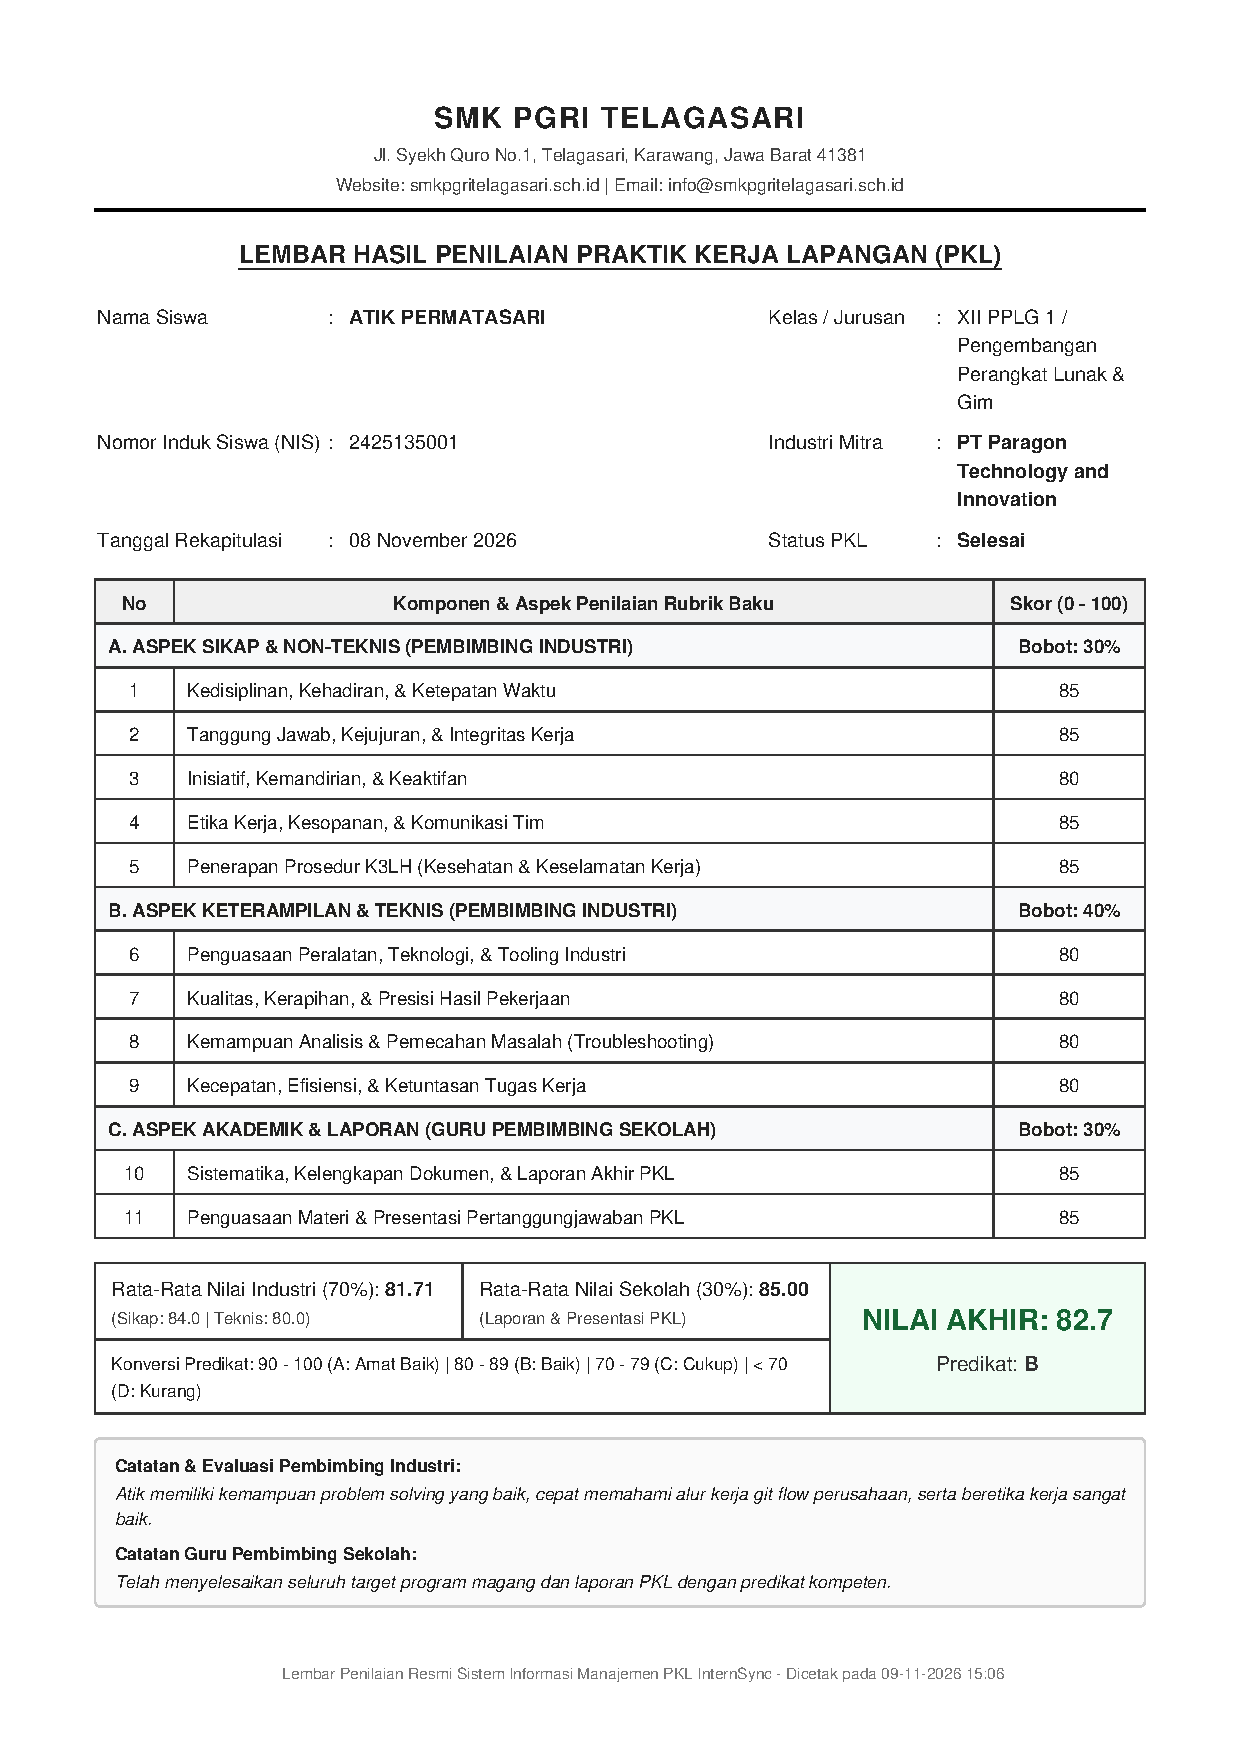
\includegraphics[page=1,width=0.90\textwidth,height=0.72\textheight,keepaspectratio,frame]{lampiran/9_Lembar_Penilaian_PKL_Siswa.pdf}
\captionof{figure}{Lembar Penilaian PKL Siswa}\label{fig:lampiran-07}
\end{center}
\clearpage

\begin{center}
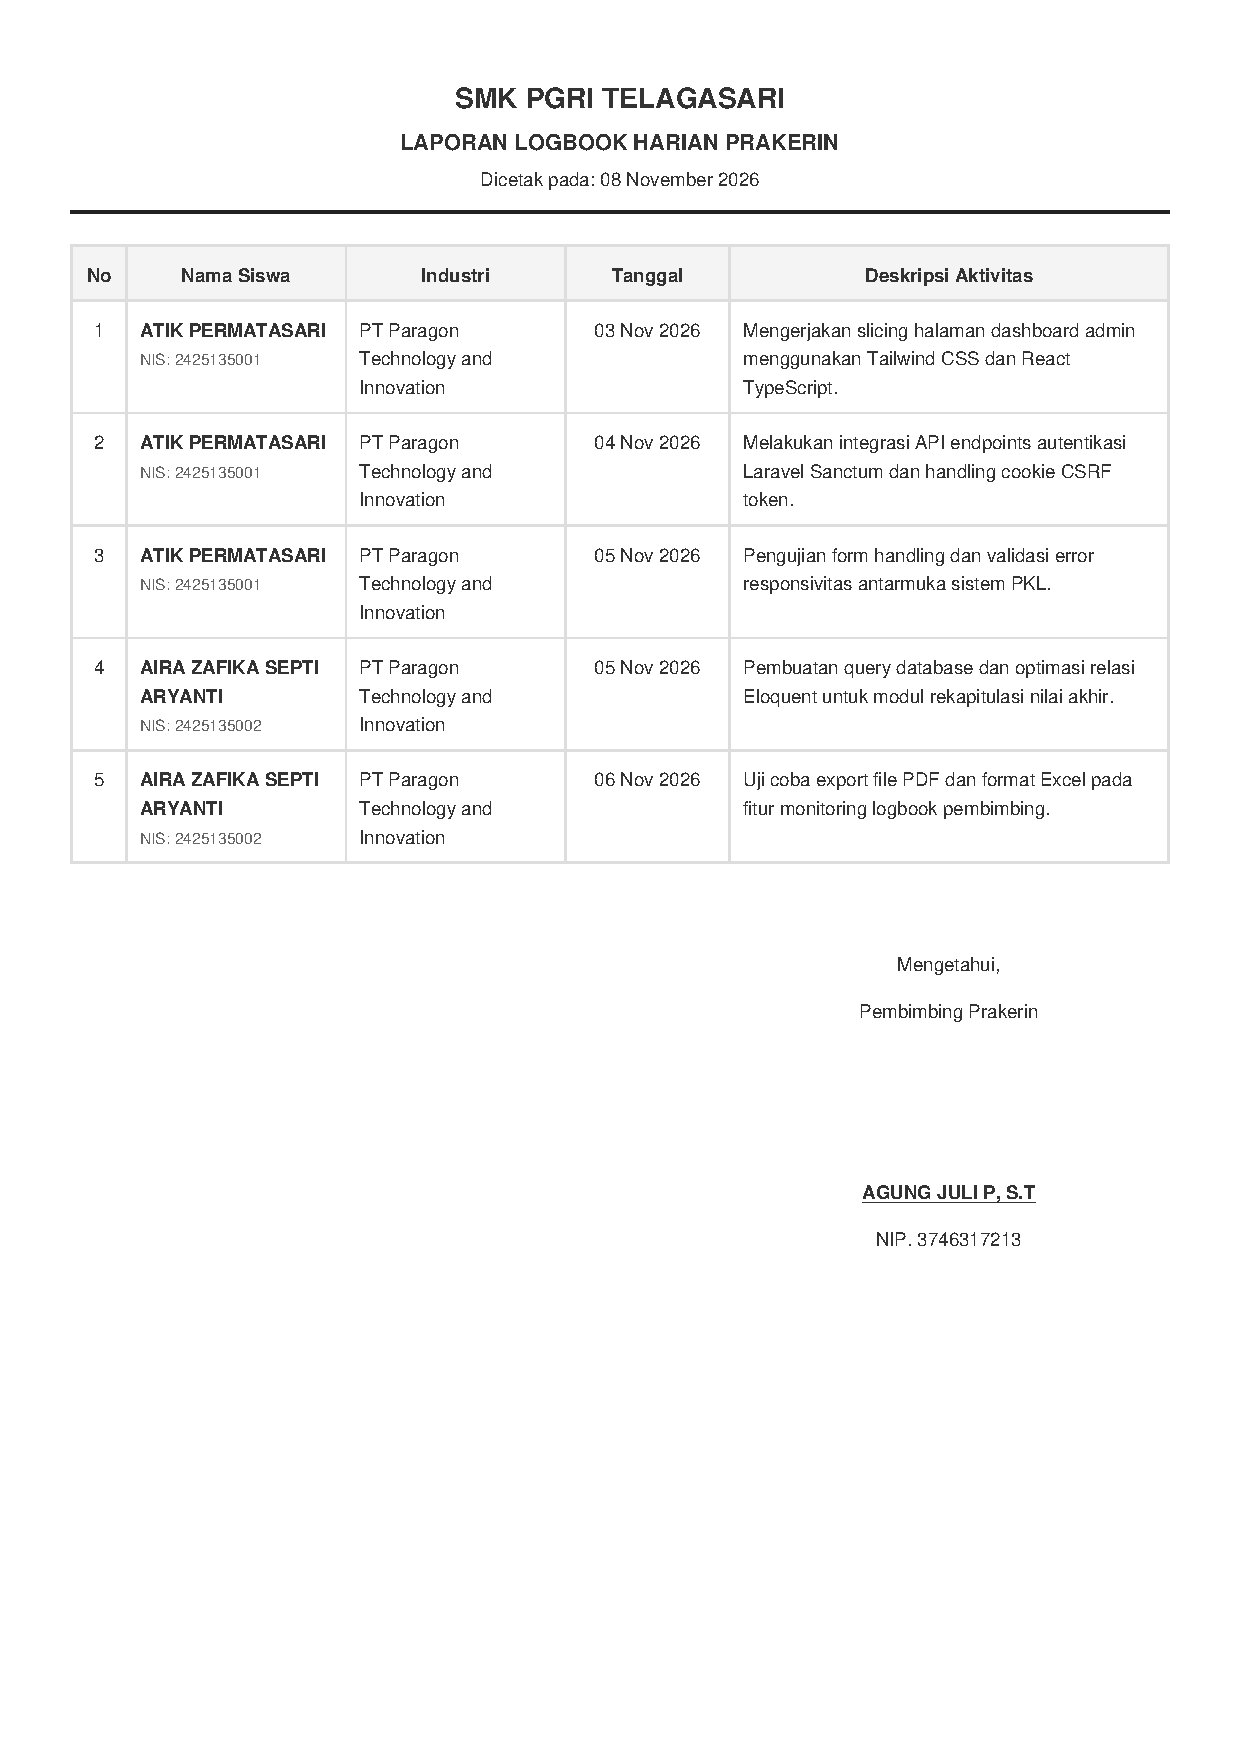
\includegraphics[page=1,width=0.90\textwidth,height=0.72\textheight,keepaspectratio,frame]{lampiran/10_Laporan_Rekap_Logbook_Siswa.pdf}
\captionof{figure}{Laporan Rekapitulasi Logbook Siswa}\label{fig:lampiran-08}
\end{center}
\clearpage

\section*{Tangkapan Layar Rekapitulasi dan Laporan}
\addcontentsline{toc}{section}{Tangkapan Layar Rekapitulasi dan Laporan}

\begin{center}
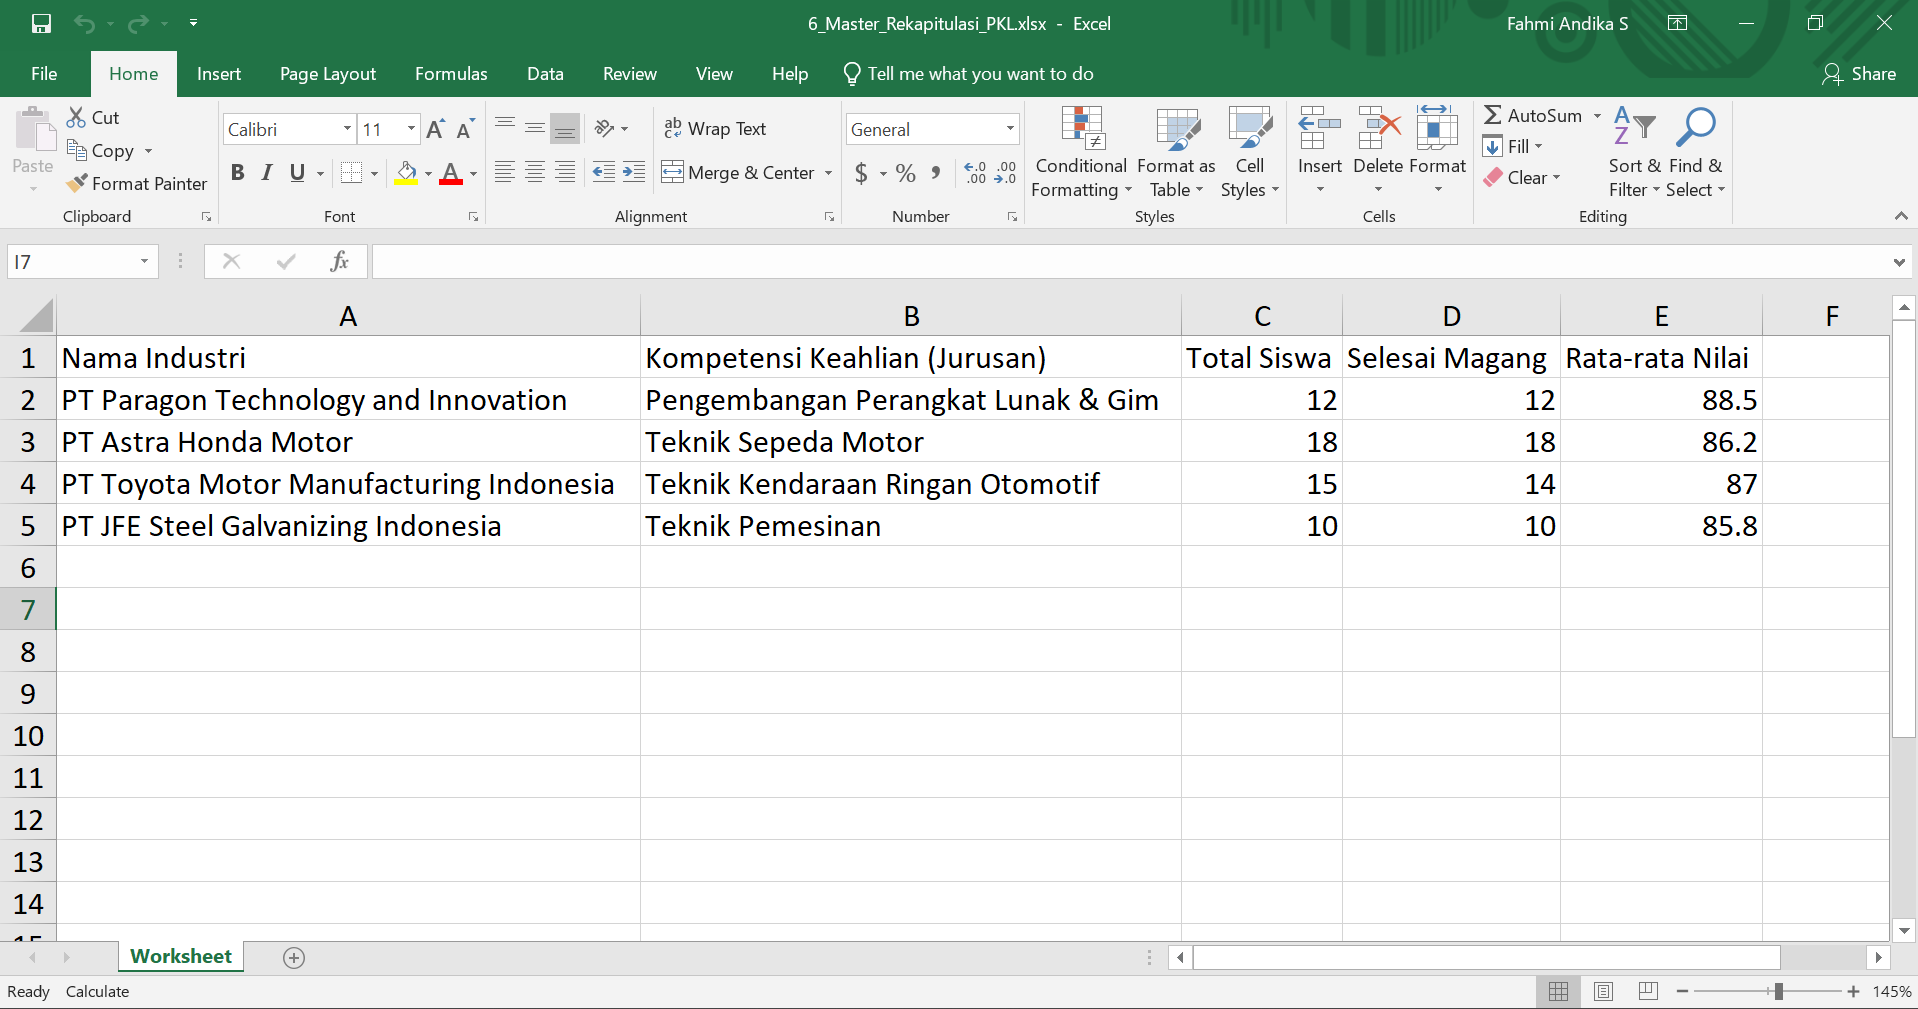
\includegraphics[width=0.94\textwidth,height=0.36\textheight,keepaspectratio]{lampiran/6_Master_Rekapitulasi_PKL.png}
\captionof{figure}{Tangkapan layar Master Rekapitulasi PKL}\label{fig:lampiran-09}
\end{center}
\medskip
\begin{center}
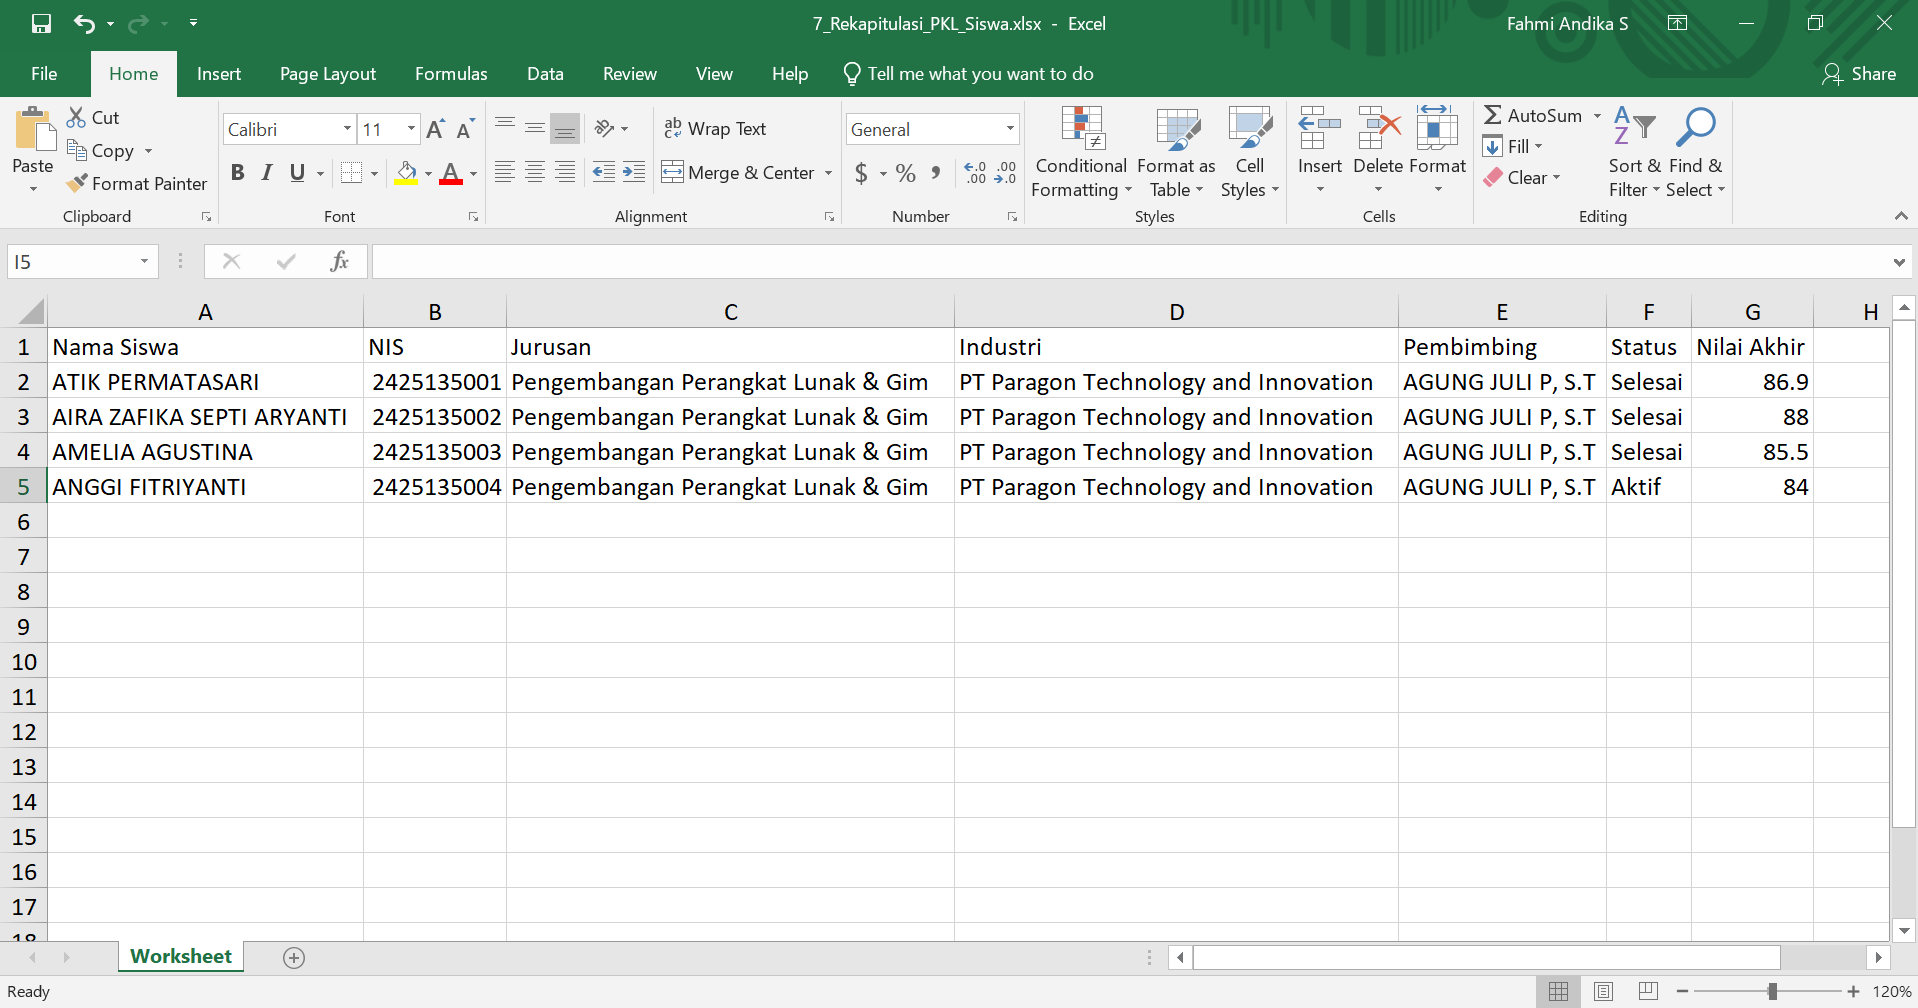
\includegraphics[width=0.94\textwidth,height=0.36\textheight,keepaspectratio]{lampiran/7_Rekapitulasi_PKL_Siswa.png}
\captionof{figure}{Tangkapan layar Rekapitulasi PKL Siswa}\label{fig:lampiran-10}
\end{center}
\clearpage

\begin{center}
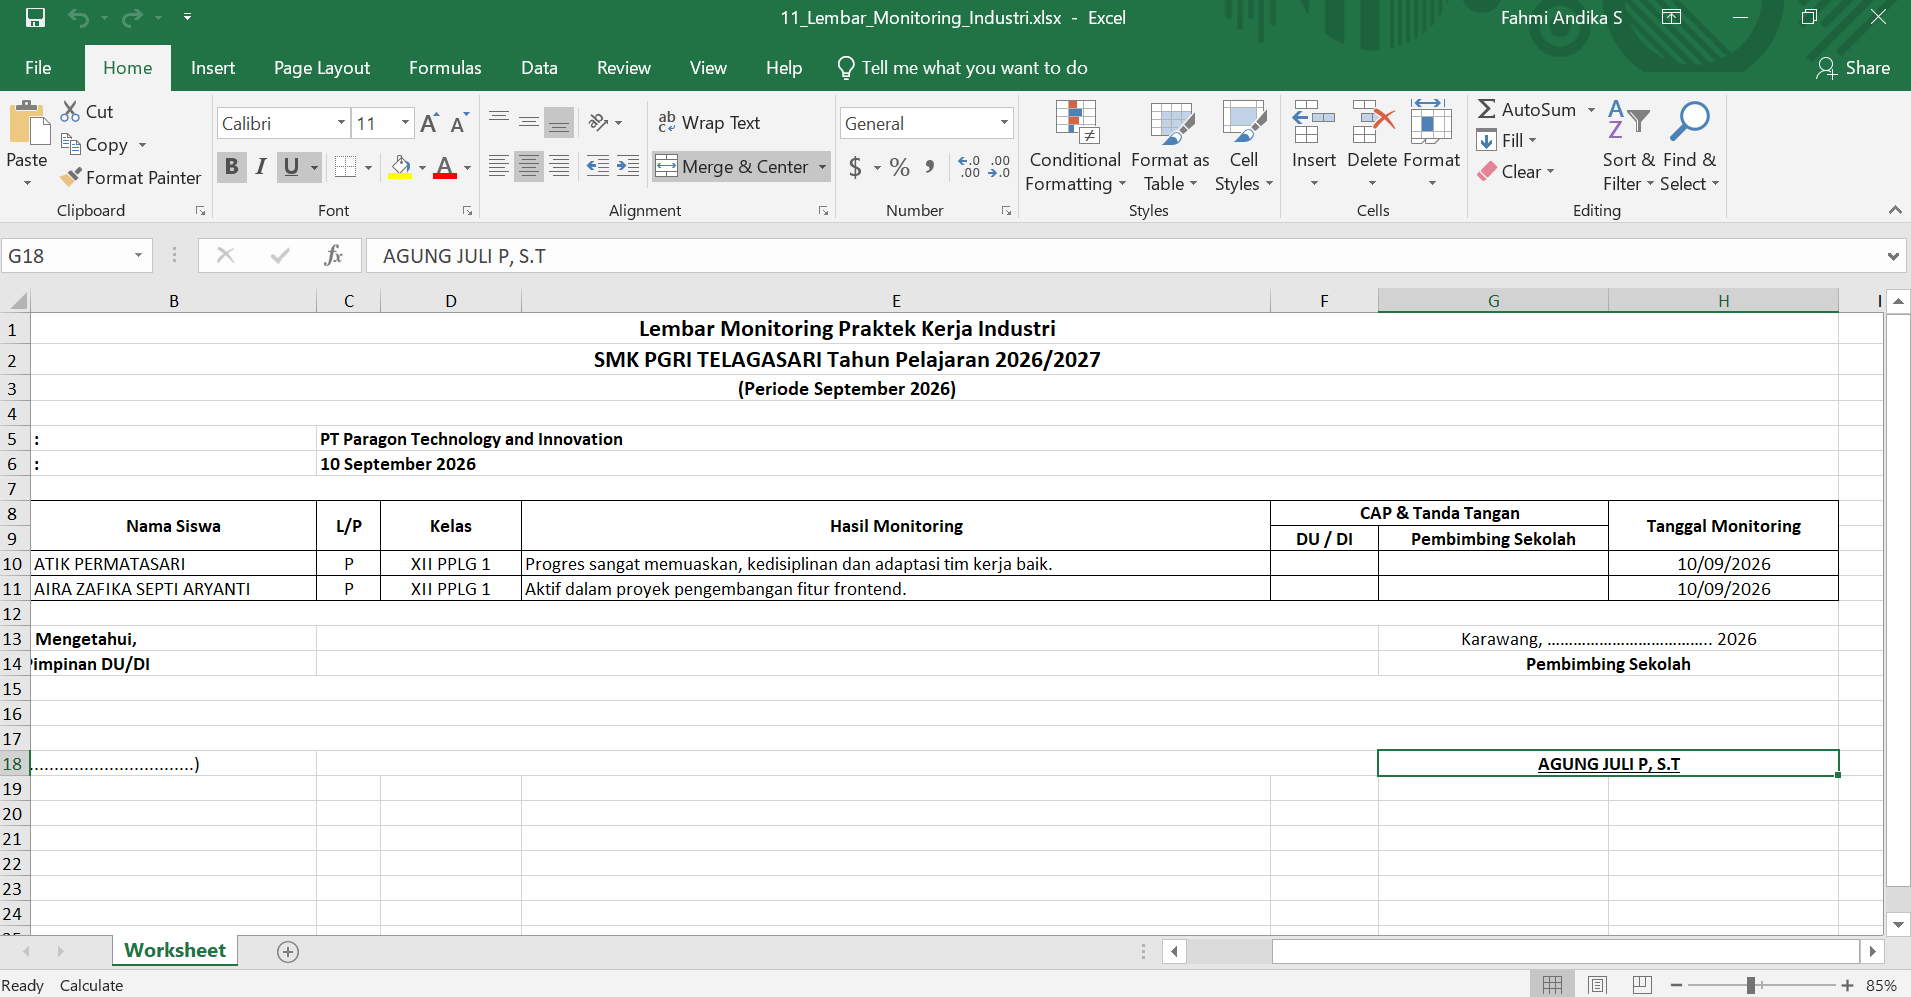
\includegraphics[width=0.94\textwidth,height=0.36\textheight,keepaspectratio]{lampiran/11_Lembar_Monitoring_Industri.png}
\captionof{figure}{Tangkapan layar Lembar Monitoring Industri}\label{fig:lampiran-11}
\end{center}
\medskip
\begin{center}
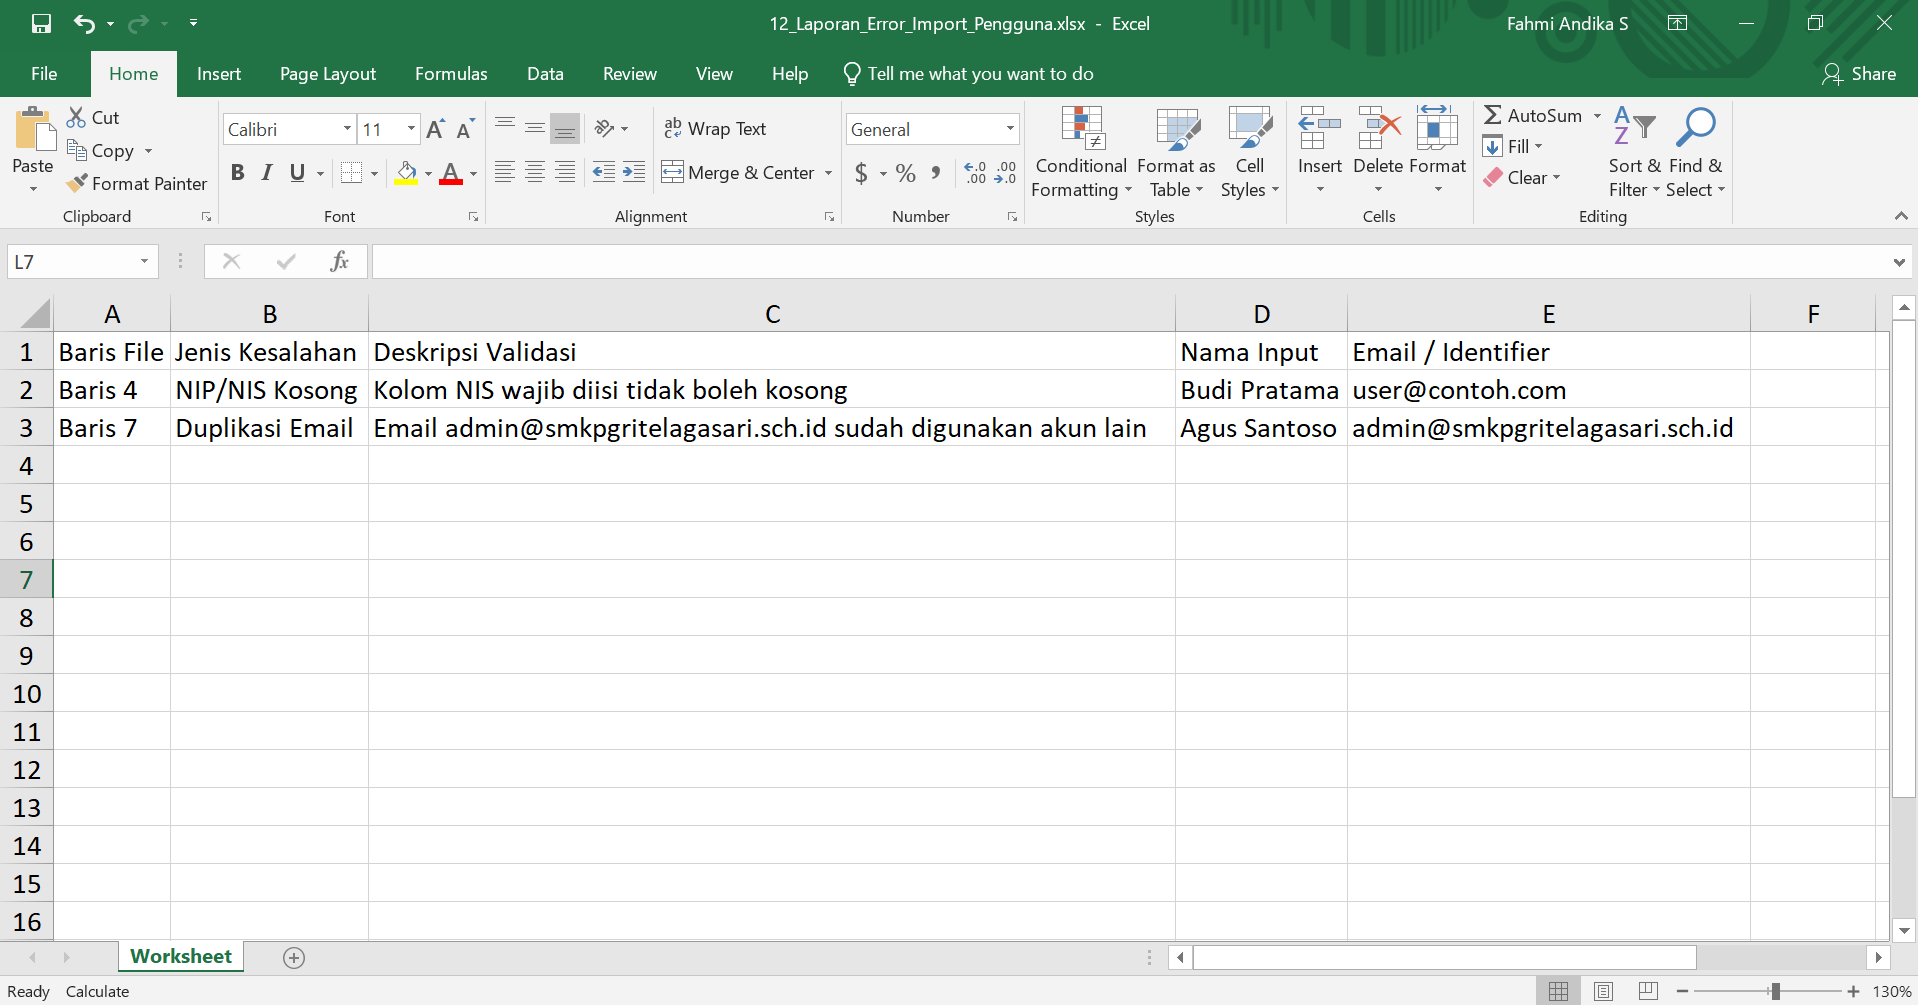
\includegraphics[width=0.94\textwidth,height=0.36\textheight,keepaspectratio]{lampiran/12_Laporan_Error_Import_Pengguna.png}
\captionof{figure}{Tangkapan layar Laporan Kesalahan Impor Pengguna}\label{fig:lampiran-12}
\end{center}


\end{document}